% ===== INICIO DEL PREÁMBULO =====

\documentclass[grade,oneside,a4paper]{udelar} % Poner msc para Maestría, dsc para Doctorado.

\usepackage[
acronyms, 											 %utiliza el glosario de acronimos.
nohypertypes={acronym,notacion,simbolos,glosario},   %quita los links en el texto al glosario.
%nonumberlist,                                       %quita los links en los glosarios al texto.
nogroupskip,                                         %quita los espacios entre diferentes grupos dentro de un glosario.
nopostdot, 											 %quita el punto final en los acrónimos         .                           
]{glossaries}

\hypersetup{ colorlinks = true } % false para imprimir, true para ver.

% Ver los documentos de estilos bibliográficos para editar estas siguientes 2 líneas.
\usepackage{natbib} % Para algunos estilos bibliográficos
\bibliographystyle{estilos_bibliograficos/natbib/apalike}

 \usepackage{makeidx}

\usepackage{eurosym}
\usepackage{enumitem}
\usepackage{longtable}
\usepackage{algorithm}
%\usepackage{algorithmic}
\usepackage{algorithmicx}
\usepackage{algpseudocode}
\usepackage{subcaption}

\loadglossary

% A su vez, la clase udelar.cls ya tiene los siguientes paquetes cargados automáticamente, que podrían ser de interés saber para el usuario:
% 
% {color},{hyphenat},{appendix},{lastpage},{babel},{inputenc},{amsmath,amssymb},{ifthen},{graphicx},{caption}
% {setspace},{tabularx},{eqparbox},{ltxcmds},{titletoc},{xcolor},{lineno},{xwatermark}
 
% Si se quieren agregar más paquetes, se recomienda colocarlos a partir de esta linea y antes de \begin{document}.



% ===== FIN DEL PREÁMBULO =====

% ===== INICIO DEL DOCUMENTO =====

\begin{document}

% \title{%
%     PARKIBIP \\
%   {\Large Retroalimentación activa en la marcha de personas con Enfermedad de Parkinson}\\[1ex]
%   {\Large Active feedback in the gait of people with Parkinson's disease }%
% }
  \title{PARKIBIP}
  \subtitle{Retroalimentación activa en la marcha de personas con Enfermedad de Parkinson}
  \institutelogo{0} % Carga cantidad de logos seleccionados, con máximo de 3 logos.
  \author{Carlos Enrique}{Huerta Santana}
  \author{Samuel}{Sainz Sanchez}

   \director{}{Franco}{Simini}{Prof.}
   \codirector{}{Antonio}{Lopez}{Prof.}  % Comentar estas líneas si no son necesarias.
%   \codirector{Prof.}{Nombre del 2do Codirector}{Apellido}{D.Sc.}
%   \codirector{Prof.}{Nombre del 3er Codirector}{Apellido}{D.Sc.}
%   \directoracademico{Prof.}{Nombre del Director Académico de Tesis}{Apellido}{D.Sc.}

  \examiner{Prof.}{Nombre del 1er Examinador}{Apellido}{D.Sc.}
  \examiner{Prof.}{Nombre del 2do Examinador}{Apellido}{Ph.D.}
  \examiner{Prof.}{Nombre del 3er Examinador}{Apellido}{D.Sc.}
  \examiner{Prof.}{Nombre del 4to Examinador}{Apellido}{Ph.D.}
  \examiner{Prof.}{Nombre del 5to Examinador}{Apellido}{Ph.D.}
  
  \graduatename{Ingeniería en Computación}
  \institute{Núcleo de Ingeniería Biomédica de las Facultades de Medicina e Ingeniería}{NIB}  % La primer institución es la principal.
  \institute{Facultad de Ingeniería}{FING}  % Agregar copias de esta línea para agregar instituciones.
  \graduatelocation{Montevideo}{Uruguay}
  
  
  \date{29}{11}{2020} % Fecha del documento.

  \keyword{Análisis de la marcha}
  \keyword{Unidad de medición inercial}
  \keyword{Sensores wereables}
  \keyword{Biorretroalimentación}
  \keyword{Enfermedad de Parkinson}
  
  \foreignkeyword{Gait analysis}
  \foreignkeyword{Inertial measurement unit}
  \foreignkeyword{Wereables sensors}
  \foreignkeyword{Biofeedback}
  \foreignkeyword{Parkinson desease}
        
  \maketitle  % Comando que genera el título de la tesis.

  \frontmatter  % Comando que genera la portadilla, el catalogo y el tribunal de evaluación. NO COMENTAR
  
  \dedication{A quienes batallan día a día con la enfermedad de Parkinson.}


  \chapter*{Agradecimentos}

El presente trabajo fue realizado bajo el acompañamiento de los profesores Franco Simini y Antonio López Arredondo, pertenecientes al Núcleo de Ingeniería Biomédica de las Facultades de Medicina e Ingeniería, Universidad de la República - URUGUAY. Gracias por su amabilidad, dedicación e ideas.

Un trabajo de investigación es siempre fruto de ideas, proyectos y esfuerzos previos que corresponden a otras personas. En este caso los mas sinceros agradecimientos al D.Sc. Biomédicas Darío Santos y a la Lic. en Fisioterapia Macarena Vergara, que a su vez, formaron parte del equipo interdisciplinario del proyecto PARKIBIP.

Asimismo, se agradece al Prof. Ing. en Computación Sebastian Pizard, de la Facultad de Ingeniería, por la orientación y atención en la realización de la Revisión Sistemática Basada en Evidencia Científica.

El agradecimiento especial a los miembros de la Asociación Uruguaya de Parkinson -AUP-, encabezados por su presidente Ana Maria Martinez, por la colaboración en la investigación. Gracias por la predisposición, amabilidad y empeño en forjar una mejor calidad de vida para con los enfermos de Parkinson.

Finalmente, resta agradecer el apoyo vital que ofrecen las personas que nos estiman, sin el cual no tendríamos la fuerza y energía que nos anima a crecer como personas y como profesionales.

Los más sinceros agradecimientos.
  \epigrafe{{\normalfont{}} Our challenges don't define us. Our actions do.}{- Michael J. Fox}


  \begin{abstract}

% Contexto 
La alteración de la marcha es el síntoma primario de un enfermo de Parkinson, causando la pérdida de independencia en los sujetos afectados a raíz de caídas, temblores y la rigidez en el movimiento. Durante las sesiones terapéuticas los estímulos externos pueden mejorar las características de la marcha.

% Objetivo 
Este proyecto tiene como objetivo la implementación de PARKIBIP, un sistema de biorretroalimentación, que le permita al enfermo una rehabilitación personal orientada a prolongar el trabajo del terapeuta en su vida cotidiana. 

% Qué se hizo 
Por lo tanto, se realizó una revisión sistemática basada en evidencia científica, que identifica todo el material relevante respecto al uso de dispositivos IMU para analizar la marcha de las personas. En base a la síntesis de estos resultados, se ingenió, diseñó y desarrolló un sistema portable capaz de procesar las mediciones arrojadas por los IMU en tiempo real. Así, detectar las fases de la marcha del paciente y estimularlo a través de sonido y/o vibración, según reglas clínicas pre-definidas por el equipo multidisciplinario de Ingeniería Biomédica. 

% Resultados y conclusiones

Se construyó una herramienta que permite avanzar en el campo de la biomecánica hacia el entendimiento de cómo los estímulos externos favorecen la marcha de las personas con enfermedad de Parkinson. Las pruebas arrojaron excelentes resultados; en promedio se realizaron 20 sesiones, detectando la cantidad exacta de pasos para un 95\% de éstas. Además, PARKIBIP fue evaluado frente a un sistema modelo, obteniendo un error cuadrático medio (RSME) entre las velocidades instantáneas de 0.021.

En conclusión, PARKIBIP es una herramienta eficaz y de gran utilidad para el terapeuta y el paciente. Tanto para retroalimentar la marcha del sujeto afectado por la enfermedad de Parkinson de forma automática, así como también efectuar un análisis objetivo de la marcha del mismo.

\end{abstract}
  \begin{foreignabstract}

Gait disorders is the primary symptom of Parkinson's patients, causing loss of independence in affected subjects as a result of falls, tremors, and stiffness in movement. During therapeutic sessions external stimuli can improve gait characteristics.

The objective of this project is to implement PARKIBIP, an active biofeedback system, which allows the patient a personal rehabilitation aimed at prolonging the work of the therapist in his daily life.

Therefore, a systematic review based on scientific evidence was carried out, which identifies all relevant material regarding the use of IMU devices to analyze people's gait. Based on the synthesis of these results, a portable system capable of processing the measurements produced by the IMUs in real time was devised, designed and developed. Thus, detect the phases of the patient's gait and stimulate it through sound and vibration, according to clinical rules pre-defined by the multidisciplinary Biomedical Engineering team.

A tool was built that allows progress in the field of biomechanics towards the understanding of how external stimuli favor the gait of people with Parkinson's disease. The tests yielded excellent results; On average, 20 sessions were carried out, detecting the exact number of steps for 95 \% of them. Furthermore, PARKIBIP was evaluated against a model system, obtaining a mean squared error between the instantaneous speeds of 0.021.

In conclusion, PARKIBIP is an effective and useful tool for the therapist and the patient. Both to provide automatically feedback during the gait of the subject affected by Parkinson's disease, as well as to carry out an objective analysis of the patient's progress. 

\end{foreignabstract}
  
  
%  \listoffigures	         % Lista de figuras
%  \listoftables	         % Lista de tablas
  
  %\listadesimbolos 		     % Lista de símbolos
  %\listadenotaciones 	     % Lista de notaciones
 % \listadesiglas 		     % Lista de siglas

  \tableofcontents           % Tabla de contenidos

  \mainmatter % Comando que genera las listas y capítulos. NO COMENTAR
  
  
  \chapter{Introducción}

\section{La enfermedad de Parkinson}

% Descripción de la enfermedad 
La enfermedad de Parkinson (EP) es un trastorno neurodegenerativo multisistémico que afecta al sistema nervioso central (SNC) provocando la aparición de síntomas motores y no motores \cite{E2004}. Causado por la deficiencia de un neurotransmisor, denominado \gls{dopamina} (DA), en el cual la pérdida progresiva de neuronas de dopamina -sito en el mesencéfalo- con la consecuente desaparición dopaminérgica de los ganglios basales, dan lugar a diversos trastornos (i.e. trastornos del movimiento y marcha, fragilidad cognitiva y emocional, alteraciones de la memoria, factores atencionales, entre otros). Es una enfermedad crónica -es decir, que persiste durante un extenso período de tiempo- y progresiva, lo que significa que sus síntomas empeoran con el tiempo \cite{E2004}.  

% Síntomas 
La alteración de la marcha es el síntoma primario del trastorno \cite{Jankovic}, y junto con las caídas causa pérdida de independencia en los sujetos afectados \cite{Ashburn}. Se caracteriza por deficiencias motoras, que incluyen temblor en las extremidades, aumento de la rigidez de las mismas, alteraciones de los parámetros espacio-temporales y fases de la marcha (p. ej. disminución de la longitud del paso y la velocidad de la marcha, variabilidad de zancada a zancada, ralentización del movimiento, marcha arrastrada o un inicio de marcha retrasado) \cite{Rogers,Stamatakis,Hausdorff,Lord}. Asimismo, la interrupción paroxística de la zancada o una marcada reducción en el avance hacia adelante del pie, llamado congelación de la marcha o FOG (del ingles, Freezing of gait) es un evento habitual, que afecta gravemente la calidad de vida, aumenta el riesgo de caídas y fracturas en los sujetos afectados \cite{Perez-Lloret2014,Bloem2004}.

% Algo de Cifras. Población afectada 
Al momento, es la segunda enfermedad neurodegenerativa más frecuente después de la enfermedad de Alzheimer y se estima una predominancia luego de los 60 años \cite{GOMEZGONZALEZ2019396,CHAVEZ-LEON2013}.
En el año 2005, en las cinco naciones más pobladas de Europa occidental -Alemania, Francia, Reino Unido, Italia, y España- y las diez más pobladas del mundo -China, India, Estados Unidos, Indonesia, Brasil, Pakistan, Bangladesh, Rusia, Nigeria y Japón-, que representan 2/3 de la población mundial, el número de personas con EP mayores de 50 años estaba entre 4.1 y 4.6 millones -10 de cada 100 mil habitantes de estos países-. Se espera que este número se duplique para el 2030 \cite{Dorsey2007ProjectedNO}.
A principios del año 2018, un estudio de prevalencia de la EP en Norte América -California, Minesota, Ontario y EE.UU.- para las personas con edad mayor o igual a los 45, estimó que existían alrededor de 680.000 individuos con la EP para el 2010 -equivalente a 477 casos cada 100.000 habitantes mayores de 45-, que ese número aumentaría a unos 930.000 aproximadamente para el 2020 -652 casos cada 100.000- y 1.238.000 para el 2030 -868 sujetos afectados cada 100.000- \cite{Marras2018}. La tendencia creciente, destaca la importancia de optimizar el cuidado y el tratamiento para las personas con EP.
Valga como ejemplo un estudio poblacional realizado en Uruguay (Migues, Canelones) entre los años 1993 y 1995 -única evidencia para Uruguay recuperada-, la prevalencia de la EP alcanzó los 136 casos cada 100.000 habitantes \cite{AljanatiR2012}. 

\section{Evaluación y tratamiento de la enfermedad de Parkinson}
% Problemas en Tratamientos actuales
% Farmacológico, su pérdida de eficacia y efectos secundarios que también son los motores
En la actualidad, el tratamiento clínico de la EP se encuentra segmentado en farmacológico, quirúrgico y rehabilitador. Todas las terapias existentes para el manejo de los síntomas, basadas en el uso de fármacos dopaminérgicos, como la L-Dopa (levodopa) y agonistas de los receptores de dopamina, han demostrado una pérdida de eficacia a lo largo del tiempo. Por cierto, se han asociado con una variedad de efectos secundarios que incluyen \gls{discinesias} y fluctuaciones motoras, que pueden incluso empeorar las deficiencias motoras propias de la enfermedad \cite{Parisi2016}. 

% Fisio y reha
De manera alternativa, para lidiar con la carencia de dopamina, la fisioterapia y la rehabilitación pueden ser efectivas para contrarrestar las deficiencias motoras.

%Reeducar la marcha
En este sentido, la rehabilitación favorece a reinstriur la marcha para lograr mayor autonomía del paciente, prolongar la funcionalidad, reducir la incapacidad motora y desarrollar estrategias para conservar la independencia en las \gls{actividades_de_la_vida_diaria} esenciales. La practica por excelencia, es la aplicación de estímulos externos del tipo auditivos (i.e. metrónomos, golpes rítmicos) o visuales (i.e. líneas perpendiculares, aros marcados en el suelo) con el fin de mejorar la marcha del paciente. Aunque la evidencia científica en relación a la reeducación de la marcha mediante estímulos externos es limitada, ciertos investigadores han reportado que (i) el \gls{SNC} puede verse afectado a través de  la aplicación de estímulos (i.e. táctiles, propioceptivos, auditivos, visuales, entre otros) \cite{Moros2000}, (ii) es posible generar patrones oportunos del ciclo de la marcha \cite{MorrisME1994,Morris1996}, (iii) la propiedad adaptativa del encéfalo para con distintos contextos \cite{Garces2014} y (iv) la recuperación de las características de la marcha y parámetros espacio-temporales mediante el entrenamiento con señales visuales y/o auditivas --de estos pacientes \cite{Ostrosky2000,PALACIOSNAVARRO201649,Mille2012} \cite{Moros2000,Dias2017TREINODM,Almeida2012}.
        
%Evidencia con estímulos
%Evaluación clínica más objetiva y el porqué es importante
%Necesidades
%Dificultades existentes -hoy-
%Uso de escalas subjetivas MDS-UPDRS

%evaluacion clinica        
Los neurólogos solo pueden confiar en observaciones cualitativas en sesiones esporádicas, de corta duración y basadas en su experiencia. Lograr una evaluación clínica con resultados confiables puede ser muy complejo y poco práctico, en virtud de las siguientes limitaciones:
\begin{itemize}
    \item Supervisión continua de los sujetos afectados por parte del personal médico.
    \item Auto-informes realizados por los mismos pacientes -afectado por el sesgo del recuerdo y probablemente sea subjetivo-.
    \item Presencia física de los pacientes a un entorno clínico donde se pueda obtener la evaluación -limitaciones de acceso (i.e condición del paciente, traslados), disponibilidad del médico o laboratorio-.
    \item Evaluación de escalas semi cuantitativa -intrínsecamente subjetivo, con una significativa variabilidad entre los evaluadores en las puntuaciones \cite{Parisi2015}-.
    \item Personal especializado.
    \item Laboratorio de marcha especializado -equipo de alto costo, limitado y compartido entre patologías-.
    \item Mucho tiempo -difícil de lograr en sesiones clínicas-.
\end{itemize}

% Cierre de problemas
La cualidad progresiva de la enfermedad, conlleva a que las características motoras se vuelven cada vez más incapacitantes y las características no motoras menos tratables (por ejemplo, la demencia), acentuando la problemática de la enfermedad. Asimismo, los trastornos de la inestabilidad postural y las alteraciones de la marcha, no se traducen únicamente en alteraciones de aspectos cinemáticos como los mencionados; sino también en aspectos relacionados con su variabilidad: manifestaciones clínicas que de forma progresiva causan limitaciones en las funciones del paciente impactando directamente en su calidad de vida y restringiendo tanto su actividad como su participación social \cite{DILLMANN2014882,MUNOZHELLIN2013190,FernandezDelOlmo2004,GOMEZGONZALEZ2019396}.

De este modo, contar con una evaluación clínica precisa y un seguimiento continuo, es fundamental para identificar una terapia efectiva; conforme a lograr una evaluación cuantitativa más objetiva de la gravedad de los síntomas de la EP, determinar con mayor precisión el grado de progreso de la enfermedad, ajustar la medicación en la atención clínica de rutina y reinstriur la marcha en beneficio de una mejor calidad de vida para los sujetos afectados.
 
\section{Oportunidades tecnológicas de mejorar el tratamiento}
%Ing biomédica y biorretroalimentación

Los sistemas de análisis de movimiento ópticos basados en cámaras son distinguidos como el estándar de oro en la medición del movimiento \cite{Stamatakis}. Si bien son muy adecuados para medir los parámetros espacio-temporales de la marcha en términos de precisión y repetibilidad, requieren sesiones terapéuticas en un entorno de laboratorio, en compañía de personal especializado, equipo considerable y tiempo.

Los avances en los dispositivos de monitoreo \gls{Wearables} están cambiando al sector médico desde un enfoque tradicional reactivo -atención de la salud en el nivel de crisis- a un enfoque de gestión proactiva de la salud \cite{SIMIC,SEPEPE,Galnares,Olivares}; que permite posponer, descubrir y abordar dichos problemas en una etapa temprana \cite{Guo}. La implementación de sistemas basados en esta tecnología innovadora, apuntan a lograr una función terapéutica, tratando a los enfermos a través de la biorretroalimentación (del ingles, \gls{biofeedback}) \cite{Frank2010} \cite{Nonnekes,Ginis2016,Lopez2014,Rochester2010}. Esto es, supervisando las funciones fisiológicas del organismo mediante la utilización de un sistema de retroalimentación, que informa al usuario del estado de la función que se desea controlar.

En el contexto de la salud, principalmente en la EP el biofeedback es fundamental, y se refiere a la provisión de estímulos externos durante o inmediatamente después de un acto motor (p. ej. cuando el sujeto levanta el pie del suelo) que brinden soporte al usuario, estimulen el compromiso cognitivo de los sujetos y potencien los efectos del ejercicio motor \cite{Rochester2010,Nieuwboer2007,Rocha2014,Spaulding2013}. Combinando la naturaleza crónica y neurodegenerativa de la EP, el crecimiento continuo en avances tecnológicos wearables, y que la rehabilitación con ejercicios deben incorporarse a largo plazo en la rutina diaria para alcanzar la máxima eficacia \cite{Tomlinson2012,Lamotte2014}, resulta evidente el GAP clínico y la necesidad de un sistema portable de biofeedback de la marcha en la EP. Cuyo propósito sea aumentar el control voluntario sobre los procesos fisiológicos que de otro modo estarían fuera de la conciencia y/o bajo un control menos voluntario; es decir, reeducar al paciente en rehabilitación a manipular eventos no detectados de forma voluntaria mediante el biofeedback, lograr una función terapéutica superando las limitaciones mencionadas.

La marcha de las personas es un proceso complejo y cíclico que requiere la sinergia de los músculos, los huesos y el sistema nervioso \cite{SAUNDERS1953}, principalmente dirigido a mantener la posición vertical y mantener el equilibrio durante condiciones estáticas y dinámicas \cite{Ayyappa1997}. Asimismo, implica la medición, la descripción y la evaluación de parámetros de marcha (p. ej. velocidad de la marcha, la amplitud de la zancada, la cadencia) que caracterizan la locomoción humana \cite{Ribeiro2017}. La correcta discriminación de las fases de marcha es considerado un punto de partida esencial para distinguir una marcha normal de una patológica o para la evaluación del estado de recuperación de la marcha durante tratamientos de recuperación \cite{Taborri2016}.

\section{Especificación de PARKIBIP}

El presente estudio tiene como objetivo la implementación de PARKIBIP, un sistema que le permita a los pacientes con la enfermedad de Parkinson una rehabilitación personal. Durante las sesiones de fisioterapia los estímulos externos pueden mejorar las características de la marcha y PARKIBIP entonces busca emular estos estímulos en tiempo real para permitirle al enfermo una rehabilitación personal que prolongue el trabajo del fisioterapeuta en su vida cotidiana y mejore la calidad de vida de la persona afectada (i.e. ganar autonomía, estabilidad, independencia, seguridad).

La Unidad de Medición Inercial es un dispositivo que combina varios sensores como el acelerómetro, giroscopio, magnetómetro, entre otros. Estos dispositivos permiten realizar un análisis de la marcha en tiempo real y evaluación de los parámetros espacio-temporales en entornos de la vida real, interiores y exteriores, superando así las limitaciones típicas de las mediciones de laboratorio. Los IMU son más económicos y más prácticos que los sistemas \gls{gait_analysis} completos; solo se requiere una preparación relativamente rápida de los pacientes, ya que el sensor se coloca en el cuerpo por medio de una banda elástica y los datos se pueden transferir fácilmente a través de Bluetooth al software dedicado.

PARKIBIP es el resultado del trabajo de un equipo interdisciplinario a partir de la experiencia de fisioterapeutas que definen las reglas para estimular a los pacientes durante la marcha. Mediante un dispositivo electrónico wearable de bajo costo (Unidad de Medición Inercial), que combina múltiples sensores, se particiona el ciclo de marcha del usuario permitiendo identificar distintos eventos, tales como, el contacto inicial con el suelo o la fase de vuelo. Finalmente, con los eventos detectados, se aplican ciertos algoritmos matemáticos que calculan los parámetros espacio-temporales claves, y en base a un módulo clínico se estimula adecuadamente al usuario. 

\section{Organización del documento}

El documento se organiza en secciones, en donde la Sección \nameref{chap:fundamentos} incluye la revisión de la literatura, los enfoques, las teorías o conceptos pertinentes en que se fundamenta la investigación, así como guiar al lector y ofrecer herramientas analíticas o interpretativas. Dada la complejidad del análisis, se detalla los materiales, procesos y métodos empleados para su resolución en la Sección \nameref{chap:project} y \nameref{chap_RSBE}. Luego, se describe la solución propuesta en el apartado \nameref{chap:implementation}, definiendo la arquitectura y sus componentes, los algoritmos numéricos empleados, el flujo operativo del sistema PARKIBIP, entre otros conceptos relevantes. Finalmente en la Sección \nameref{chap:test_results}, se presentan las pruebas de verificación del sistema, los principales hallazgos, el modo de recolección de datos y el protocolo experimental, así como las sesiones experimentales del proyecto. A modo de epílogo, se sintetizan las posturas expuestas durante el proyecto en el Apartado \nameref{chap:conclusions}, se exponen las complejidades y limitaciones en el transcurso del proyecto. Asimismo, se efectúan contribuciones teóricas o metodológicas a la disciplina y recomendaciones para profundizar en el campo del biofeedback aplicado a la EP.
 % Se carga el capítulo Introduccion
  \chapter{Fundamentos teóricos}\label{chap:fundamentos}

\section{Enfermedad de Parkinson}

\subsection{Epidemiología y Etiología}
La \gls{enfermedad_de_Parkinson} (EP) es un trastorno neurodegenerativo multisistémico y de presentación generalmente esporádica, que afecta al sistema nervioso central provocando la aparición de síntomas motores y no motores \cite{E2004}. Es una enfermedad crónica -es decir, que persiste durante un extenso período de tiempo- y progresiva, lo que significa que sus síntomas empeoran con el tiempo. Su etiología desconocida conlleva a una patología aun mas compleja \cite{3249850720080101}; sin embargo, se cree que está relacionada con la acción e interacción de diversos factores genéticos y ambientales, que actúan como factores de susceptibilidad o precipitantes \cite{CAMPDELACREU2014541}.

Fue descrita por primera vez por James Parkinson en el año 1817 \cite{JamesParkinson2002}, siendo actualmente la segunda enfermedad neurodegenerativa más frecuente después de la enfermedad de Alzheimer, y se estima una predominancia luego de los 60 años \cite{GOMEZGONZALEZ2019396,CHAVEZ-LEON2013}. Es fundamental evaluar y cuantificar el impacto de la enfermedad en la población, particularmente en Uruguay. De esta manera, se pudo constatar que:

\begin{itemize}
    \item Alrededor del 3\% de la población mundial mayor a los 65 años padece la enfermedad de Parkinson \cite{Patel2009}, pudiendo alcanzar una prevalencia del 4\% en pacientes mayores de 80 años \cite{DeLauBreteler}
    \item En el año 2005, en las cinco naciones de Europa occidental y las diez más pobladas del mundo, representando 2/3 de la población mundial, el número de personas mayores de 50 años con EP estaba entre 4.1 y 4.6 millones. Se espera que este número ascienda entre 8.7  y 9.3 millones de parkinsonianos para 2030 \cite{Dorsey2007ProjectedNO}
    \item A principio del año 2018, un estudio de prevalencia de la EP en Norte América para las personas con edad mayor o igual a los 45 años, estimó que la prevalencia de la enfermedad era de 572 por 100.000 (intervalo de confianza del 95\%). Es decir, que habían unos 680.000 individuos en los EE. UU. con EP para el año 2010, que ese número aumentaría a unos 930.000 aproximadamente en 2020 y 1.238.000 para el año 2030 según las proyecciones de la población de la Oficina del Censo de los EE. UU \cite{Marras2018}
\end{itemize}

En cambio, no se encontró evidencia científica respecto a la prevalencia de la EP en Uruguay con datos actualizados y fiables. En el año 1993, se realizó un estudio de prevalencia de las enfermedades Neurodegenerativas donde se concluye que la prevalencia de la EP era de 1.36 casos cada 1000 habitantes \cite{AljanatiR2012}. Sin embargo, el estudio resulta arbitrario debido a la metodología utilizada, donde  en una primera fase consistió en una encuesta puerta a puerta -acotada a la ciudad de Migues, Canelones-; adecuada para la época pero obsoleta en la actualidad. Además, como se pudo ver en los estudios de prevalencia en otras regiones, la población afectada por la EP varía año a año. 

%Mas cifras
Por otro lado, el estudio reportado en \cite{Dorsey2018}, estima la carga global de la enfermedad de Parkinson entre 1990-2016, y busca identificar tendencias asociadas al trastorno (GBL, del ingles Global Burden of Disease). Según los resultados alcanzados, en 2016, 6.1 millones de individuos en todo el mundo padecían la EP, de los cuales 2.9 millones (47.5\%) eran mujeres y 3.2 millones (52.5\%) eran hombres afectados. Un total de 2.1 millones (34.4\%) de estos individuos provenían de países con un índice socio-demográfico (SDI) alto, 3.1 millones (50.8\%) de países con SDI medio o medio alto, y un 0.9 millones (14.8\%) de países con SDI medio o bajo. 

\noindent A nivel mundial, la enfermedad de Parkinson causó 211.296 muertes -93.512 mujeres y 117.784 hombres- y 3.2 millones de años perdidos debido a enfermedad, discapacidad o muerte prematura (AVAD, años de vida ajustados por discapacidad) -1.4 millones en mujeres; 1.8 millones en hombres- en 2016. Se entiende por AVADs como la suma de los años de vida perdidos (YLL, siglas en ingles, Years of Life Lost) y los años vividos con la discapacidad (YLD, siglas en ingles, Years Lost due to Disability). La figura Fig. \ref{fig:yll_yld} permite visualizar las tasas de YLL y YLD según la edad; así, el aumento relacionado con la edad fue considerablemente más pronunciado para los YLL que para los YLD, lo que sugiere que la letalidad para la EP aumenta con la edad.

\begin{figure}[H]
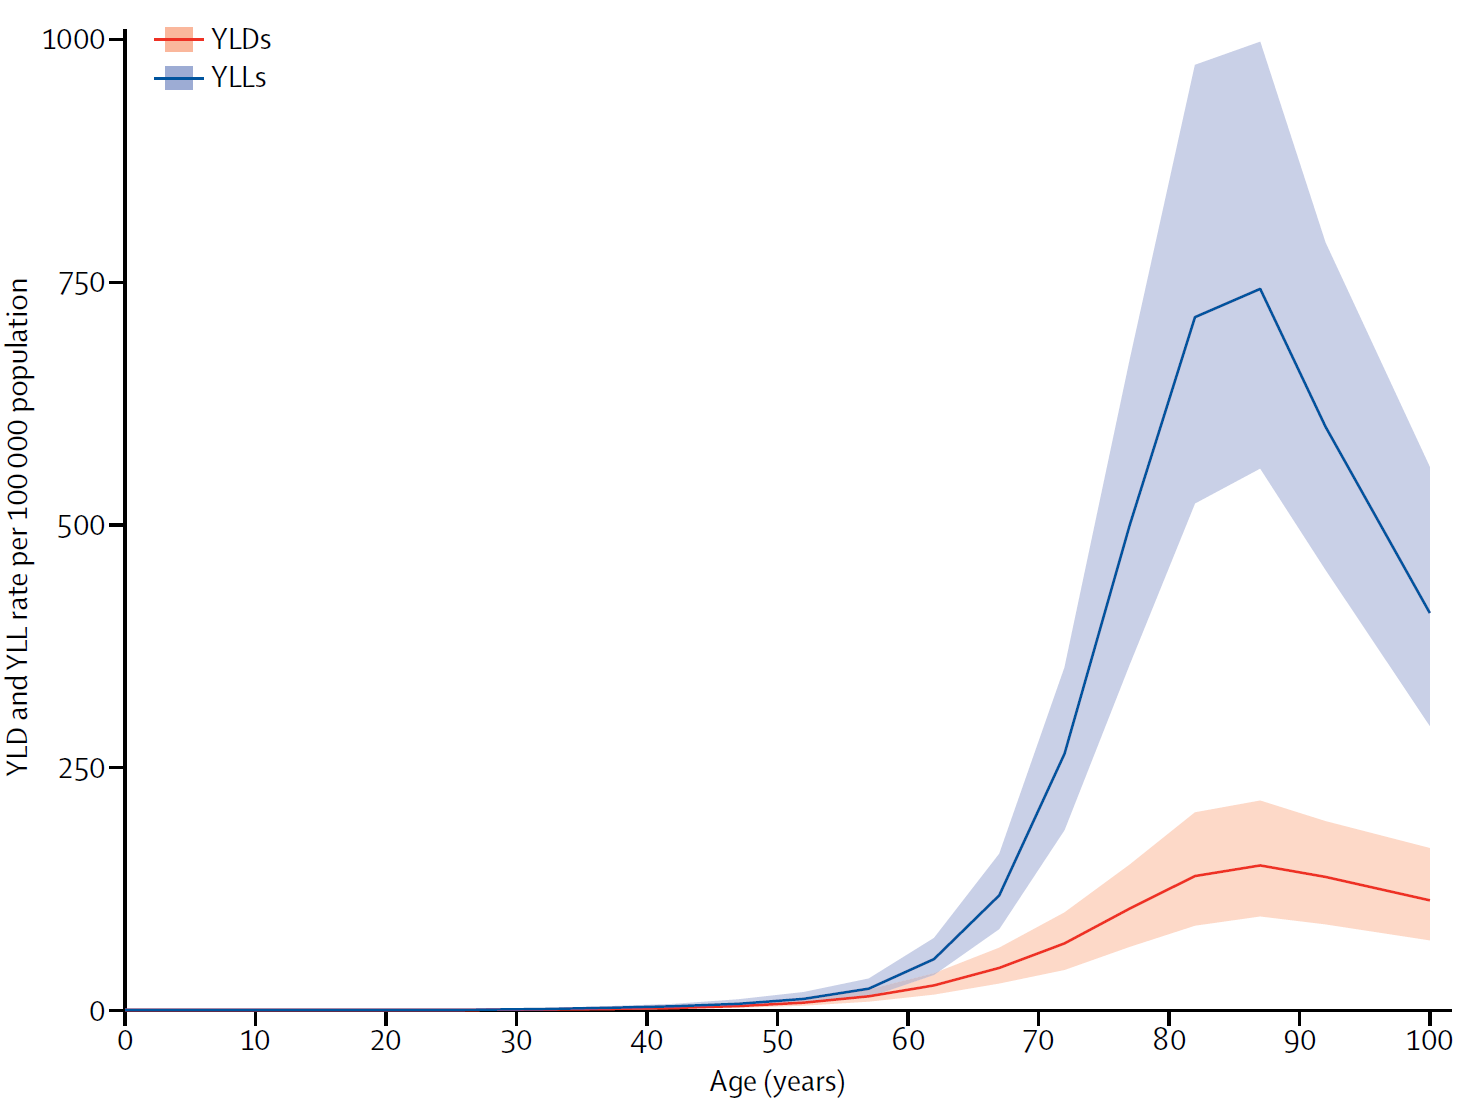
\includegraphics[width=\textwidth]{TESIS/imagenes/chap02/yll_yld.PNG}
\caption{ Tasas de años vividos con la discapacidad (YLD) y años de vida perdidos (YLL) cada 100.000 habitantes debido a la Enfermedad de Parkinson por edad, 2016. El sombreado indica intervalos de confianza del 95\%. \cite{Dorsey2018} }
\label{fig:yll_yld}
\end{figure}

\noindent En resumen, algunos hallazgos logrados fueron que:

\begin{itemize}
    \item El número de individuos con la EP en 2016 fue 2.4 veces mayor que a la de  1990. Dicho aumento no se explicó exclusivamente por un número cada vez mayor de personas adultas, ya que las tasas de prevalencia estandarizadas por edad aumentaron en un 21.7\% desde 1990 a 2016 en comparación con un aumento del 74.3\%  para las tasas brutas
    \item El número de muertes fue 2.6 veces mayor y el número de AVADs fue 2.5 veces mayor en 2016 que en 1990. Similar a la prevalencia, los aumentos no se explican solo por un número creciente de personas mayores, ya que las tasas estandarizadas por edad aumentaron en un 20\% tanto para las muertes como los AVADs
    \item La EP era poco frecuente antes de los 50 años de edad. La prevalencia en 2016 aumentó con la edad a partir de entonces y alcanzó un máximo entre los 85 y los 89 años (1.7\% para hombres; 1.2\% para mujeres) y disminuyó después de esa edad
\end{itemize}

\noindent La tabla Tab. \ref{ep_paises} ilustra los indicadores de defunciones, de prevalencias y las tasas AVADs a nivel mundial y en América del sur, especialmente Uruguay.

\begin{table}[H]
\begin{center}
\caption{Defunciones, prevalencia y AVADs (años de vida ajustados por discapacidad) para la enfermedad de Parkinson en 2016, y cambio porcentual entre 1990 y 2016 en las tasas estandarizadas por edad y por ubicación. \cite{Dorsey2018}} \label{ep_paises}
\hspace*{-2cm}%
\begin{tabular}{|p{2cm}|p{2cm}|p{2cm}|p{2cm}|p{2cm}|p{2cm}|p{2cm}|}
\hline
 & \multicolumn{2}{c|}{Decesos} & \multicolumn{2}{c|}{Prevalencia} & \multicolumn{2}{c|}{AVADs} \\
\hline
& En 100.000 (2016) & Tasa de cambio (1990–2016) & En 100.000 (2016) & Tasa de cambio (1990–2016) & Cantidad (2016) & Tasa de cambio (1990–2016) \\
\hline
Global & 2,83 & +19,5\% & 81,2 & +21,7\% & 3.234.514 & +22,1\% \\
\hline
América del sur & 0,98  & +3,1\% & 28 &  +5,4\% & 57.932 & +4,3\% \\
\hline
Uruguay & 8,38 & +7,1\% & 183,6 & +10,9\% & 3.775 & +8,2\% \\ \hline
\end{tabular}
\end{center}
\end{table}

\subsection{Sintomatología de la patología}

La alteración de la marcha es el síntoma primario del trastorno \cite{Jankovic}, y junto con las caídas causa pérdida de independencia en los sujetos afectados \cite{Ashburn}. Se caracteriza por deficiencias motoras, que incluyen esencialmente \cite{Rogers,Stamatakis,Hausdorff,Lord}: 
\begin{itemize}
    \item Temblor en las extremidades
    \item Aumento de la rigidez de las mismas
    \item Alteraciones de los parámetros espacio-temporales y fases de la marcha (p. ej. disminución de la longitud del paso y la velocidad de la marcha, variabilidad de zancada a zancada, fases de marcha)
    \item Ralentización del movimiento, marcha arrastrada o un inicio de marcha retrasado 
\end{itemize}

Otro evento frecuente, es la congelación de la marcha (FOG, del ingles, Freezing of gait), dado por una interrupción paroxística de la zancada o una marcada reducción en el avance hacia adelante del pie, que afecta gravemente la calidad de vida, aumenta el riesgo de caídas y fracturas en los sujetos afectados \cite{Perez-Lloret2014,Bloem2004}. En pacientes con EP, la investigación fisiopatológica de la FOG es bastante desafiante ya que se encuentra influenciada de manera crucial por una serie de factores cognitivos, atencionales, emocionales e incluso ecológicos \cite{Professor2008,Barthel2016}.

La cualidad progresiva de la enfermedad, conlleva a que las características motoras se vuelven cada vez más incapacitantes y las características no motoras menos tratables (p. ej. la demencia), acentuando la problemática de la enfermedad. Asimismo, los trastornos de la inestabilidad postural y las alteraciones de la marcha, no se traducen únicamente en alteraciones de aspectos cinemáticos como los mencionados; sino también en aspectos relacionados con su variabilidad, manifestaciones clínicas que de forma progresiva causan limitaciones en las funciones del paciente que impactan directamente en su calidad de vida y restringiendo tanto su actividad como su participación social \cite{DILLMANN2014882,MUNOZHELLIN2013190,FernandezDelOlmo2004,GOMEZGONZALEZ2019396}.

\subsection{Rehabilitación convencional}

En la actualidad, todas las terapias existentes para el manejo de los síntomas basadas en el uso de medicamentos dopaminérgicos, como la L-Dopa (levodopa) y agonistas de los receptores de \gls{dopamina}, han demostrado una pérdida de eficacia a lo largo del tiempo. A su vez, se han asociado con una variedad de efectos secundarios que incluyen \gls{discinesias} y fluctuaciones motoras, que pueden incluso empeoran las deficiencias motoras propias de la enfermedad.

Con el fin de lograr una evaluación cuantitativa más objetiva de la gravedad de los síntomas de la EP, determinar con mayor precisión el grado de progreso de la enfermedad, ajustar la medicación en la atención clínica de rutina o para su uso como medidas de resultados en ensayos clínicos, los neurólogos se apoyan en las escalas de evaluación semi cuantitativa, como lo es la Escala Unificada de Clasificación de la Enfermedad de Parkinson -elaborada por la Sociedad de Trastornos del Movimiento- (MDS-UPDRS, por sus siglas en ingles) \cite{Jellinger2002}. La escala MDS-UPDRS consiste en diversas partes, que buscan evaluar los síntomas motores y no motores a través de encuestas respondidas por el paciente, y evaluaciones basadas en exámenes realizadas por un médico capacitado. La principal limitación de esta evaluación es ser intrínsecamente subjetiva, con una significativa variabilidad entre los evaluadores en las puntuaciones \cite{Parisi2015}. Además, es una tarea que requiere mucho tiempo -difícil de lograr en sesiones clínicas-, y a la vez la presencia física de los pacientes en un entorno clínico donde se pueda obtener la evaluación. El Apéndice \nameref{appendix:MDS-UPDRS} permite visualizar la evaluación clínica mediante la escala MDS-UPDRS.

\subsubsection{Fisioterapia y rehabilitación}

A medida que la enfermedad progresa, la mayoría de las alteraciones del equilibrio y la marcha se vuelven resistentes a los tratamientos farmacológicos y quirúrgicos \cite{Rubinstein2002}. En consecuencia, para sortear el déficit de dopamina, la fisioterapia y la rehabilitación (i.e. estiramiento, fortalecimiento muscular, movimientos de las extremidades con pelotas y materiales de juego, acondicionamiento en bicicleta) pueden ser efectivas para contrarrestar las deficiencias motoras \cite{Fox2008}. 

La finalidad de la terapia de rehabilitación, es mejorar o mantener la calidad de vida de los sujetos afectados conforme a aumentar la movilidad, mejorar el equilibrio, la coordinación, reeducar la marcha para lograr la autonomía del paciente. Si bien ésta terapia no detiene la progresión de la enfermedad, habilita a prolongar la funcionalidad y reducir la incapacidad motora perfeccionando la marcha, las destrezas propioceptivas y desarrollando estrategias para conservar la independencia en las \gls{actividades_de_la_vida_diaria} elementales.

De esta manera, la rehabilitación debe atender al paciente según sus necesidades, su discapacidad, el estadio evolutivo de la enfermedad y las expectativas del paciente -similar a todas las enfermedades crónicas y progresivas-. 
A modo de ejemplo, se describen las fases y actividades del tratamiento de acuerdo a su evolución y al protocolo clínico a seguir \cite{MINISTERIO2010}:

\begin{enumerate}
    \item Fase Inicial
    \begin{itemize}
        \item Prevenir y tratar la inestabilidad postural.
        \item Evaluar e identificar tempranamente los problemas relacionados con alteraciones del movimiento.
        \item Fomentar la participación del paciente con EP en programas diseñados para mejorar la condición física general. (Cardiovascular, músculo esquelética, y neuromuscular).
        \item Prevenir las deficiencias posturales, deficiencias en marcha y traslado.
        \item Tratar la debilidad muscular y/o la rigidez articular.
        \item Utilizar estrategias de movimientos a lo largo de la enfermedad.
        \item Informar y Educar en salud, acerca de la enfermedad a los pacientes, familiares y cuidadores.
    \end{itemize}   

    \item Fase de Mantenimiento
    \begin{itemize}
        \item Tratar el deterioro músculo esquelético.
        \item Reeducar marcha y traslados. Prevención de caídas.
        \item Evaluar el medio en donde se desenvuelve el paciente (entrenamiento en el hogar y comunidad).
        \item Aplicar estrategias funcionales.
        \item Evaluar la prescripción de AT e instruir en su uso adecuado.
    \end{itemize}

    \item Fase Avanzada o tardía
    \begin{itemize}
        \item Asegurar el manejo adecuado de movimiento y posición.
        \item Evitar las caídas.
        \item Prevenir lesiones trofocirculatorias y posturales.
        \item Prevenir y tratar los problemas respiratorios.
    \end{itemize}
\end{enumerate}

Otra metodología muy empleada en la fisioterapia y rehabilitación, es la aplicación de incentivos o guías externas del tipo auditivo (i.e. a modo de metrónomos o golpes rítmicos en el suelo) o visual (i.e. huellas o líneas perpendiculares marcadas en el suelo) para mejorar los trastornos de la marcha; es decir, \gls{reeducar_la_marcha}. Si bien la evidencia científica existente respecto a la reeducación de la marcha es reducida, muchas investigaciones han concluido y reportado los siguientes resultados:

\begin{itemize}
    \item Viabilidad de generación de patrones adecuados de la marcha. Según \cite{MorrisME1994,Morris1996}, es posible que los parkinsonianos en presencia de estimulación sensorial regular, generen patrones adecuados de la marcha, corroborando una mejoría en los parámetros espacio-temporales bajo el uso de estímulos externos.
    
    \item Factibilidad de incidencia sobre el \gls{SNC}. Con fundamento en el principio de que todo acto motor es una elaboración del SNC -en respuesta a múltiple información sensitivo motora, simultánea y secuencial-, en efecto, se concluye que el segundo puede verse afectado o modificado positivamente mediante diversos estímulos táctiles, propioceptivos, auditivos, visuales, entre otros \cite{Moros2000}.
    
    \item Capacidad adaptativa del encéfalo. Existe evidencia científica que comprueban las propiedades de flexibilidad y modificabilidad del cerebro en distintos contextos -durante la infancia y la adolescencia, durante la edad adulta, como también en situaciones de lesión cerebral-. Así, el encéfalo puede alterase para adaptarse a diversas circunstancias \cite{Garces2014}.
    \item Estimulación visual sobre la marcha. El Neurólogo Británico James Purdon Martin,  logró demostrar el efecto positivo de las señales visuales sobre la marcha en la EP en el año 1967. Comprobó cómo tan solo una serie de líneas de color dispuestas en el suelo -de forma perpendicular a la dirección del movimiento-, mejoraban las características de la marcha de estos pacientes  \cite{Ostrosky2000,PALACIOSNAVARRO201649,Mille2012, ilianaloyola2017}.
    \item Resultados alentadores. Sidaway -entrenamiento con señales visuales- \cite{Moros2000}, logro una mejoría duradera en la velocidad de la marcha y en la longitud del paso incrementando la estabilidad del control motor subyacente responsable de la marcha. La investigación de \cite{Dias2017TREINODM} -señales visuales y terapia convencional-, aumentó la velocidad,la longitud de zancada y la cadencia al caminar, mejoró el equilibrio y la independencia en las actividades funcionales. Las sesiones experimentales en \cite{Almeida2012}, lograron mejoras  significativas de la longitud del paso, mejorando así la velocidad de la marcha -un incremento aproximado de 10 cm/s).
\end{itemize}

Conforme a lo mencionado, lograr una evaluación clínica con resultados confiables puede ser muy complejo y poco práctico, ya que requiere una supervisión continua de los sujetos afectados por parte del personal médico, o auto-informes realizados por los mismos pacientes (lo que probablemente sea subjetivo). El aumento de las disfunciones motoras a medida que avanza la enfermedad requiere evaluar cuantitativamente y controlar las alteraciones de la marcha con el tiempo. Asimismo, los neurólogos solo pueden confiar en observaciones cualitativas en sesiones esporádicas y basadas en su experiencia. De este modo, contar con una evaluación clínica precisa de la gravedad de estos síntomas y un seguimiento continuo (p. ej. un instrumento que actuara directamente sobre el desempeño de la marcha sería de utilidad mayor), es fundamental para identificar una terapia efectiva.

 
\subsection{Nuevo paradigma de Rehabilitación}

Con fundamento en las limitaciones clínicas mencionadas en el tratamiento convencional del trastorno para identificar, evaluar y monitorear la enfermedad de parkinson, la Ingeniería Biomédica ha realizado esfuerzos para desarrollar métodos objetivos y precisos utilizando sistemas de medición de movimiento. En general, el análisis instrumentado de la marcha (\gls{gait_analysis}, por sus siglas en ingles) se emplea con frecuencia para obtener parámetros cinemáticos, cinéticos y espacio-temporales, y en efecto, lograr una imagen cuantitativa de la función de la marcha. Estos parámetros espacio-temporales son ampliamente utilizados en el contexto clínico, ya que describen objetivamente los principales eventos del ciclo de la marcha y reflejan la capacidad del paciente para cumplir una marcha adecuada (i.e la aceptación del peso, el soporte de una sola extremidad, la fase de vuelo de una extremidad (\cite{BUGANE2012129}). Específicamente, diversas investigaciones han reportado que las principales alteraciones en el GA para la EP son: 

\begin{itemize}
    \item Reducción de la longitud de la zancada, a menudo acompañada de una velocidad de caminata más baja \cite{DeSouza2011}.
    \item Intento de extender la fase de doble apoyo \cite{Sofuwa2015}.
    \item Ausencia de ``golpe de talón'', debido al típico soporte de pie plano \cite{Sofuwa2015}.
    \item Problemas para cambiar de dirección durante el giro \cite{MORRIS2001459,Nutt2011}. Girar puede ser incluso más frecuente que caminar hacia adelante, especialmente en entornos confinados como las viviendas.
    \item Dificultad para iniciar la marcha, acortamiento de la longitud del paso, poca elevación de los pies del suelo con su consecuente arrastre.
    \item Variabilidad entre los pasos. Esta variación en la duración del ciclo es una característica importante de la marcha parkinsoniana y se considera un indicador del riesgo de sufrir caídas.
\end{itemize}

En estas condiciones, los sistemas instrumentados de análisis de la marcha son fundamentales. Los sistemas de análisis de movimiento ópticos basados en cámaras (3D-GA) son reconocidos como el estándar de oro en la medición del movimiento \cite{Stamatakis}. Por ejemplo, se utilizan para medir los parámetros de la marcha con el fin de cuantificar la gravedad de la EP \cite{ROIZ2010}, y así proporcionar información esencial sobre el estado funcional de un sujeto. Estos sistemas son muy adecuados para medir las características de la marcha en términos de precisión y repetibilidad, sin embargo, requieren ejecutar las pruebas en un entorno de laboratorio con equipos de alto costo, solo se pueden usar para evaluar segmentos cortos de la marcha, requiere personal especializado, equipo considerable y tiempo.\label{parkinson:limitaciones}

Análogamente, los recientes avances en la tecnología weareable, han llevado al desarrollo de dispositivos de medición que pueden evaluar el movimiento humano utilizando sensores conectados al cuerpo con una variedad de configuraciones diferentes (i.e. frecuencia cardiaca, acelerómetro, giroscopio). Los parámetros de la marcha medidos bajo estos instrumentos, son indicadores útiles para caracterizar la EP, así como para cuantificar la gravedad de la enfermedad en los sujetos \cite{Dewey2014}. 

Teniendo en cuenta la naturaleza crónica y neurodegenerativa de la EP, e integrando el crecimiento continuo en avances tecnológicos wearables, y que la rehabilitación y la terapia con ejercicios deben incorporarse a largo plazo en la rutina diaria para alcanzar la máxima eficacia \cite{Tomlinson2012,Lamotte2014}, comprueban la existencia de un importante GAP clínico. Combinar los sistemas instrumentados de análisis de la marcha con la terapia de biorretroalimentación, para construir un sistema final de biofeedback portable -uso cotidiano y en exteriores-, accesible y de bajo costo; cuyo objetivo sea aumentar el control voluntario sobre los procesos fisiológicos que de otro modo estarían fuera de la conciencia y/o bajo un control menos voluntario. Es decir, reeducar al paciente en rehabilitación a manipular eventos no detectados de forma voluntaria mediante la retroalimentación, lograr una función terapéutica superando las limitaciones mencionadas en \ref{parkinson:limitaciones}. 

\section{Sistemas clínicos de Biofeedback}

El objetivo del presente apartado es transmitir las tendencias y la evolución en el desarrollo de la biorretroalimentación (del ingles, \gls{biofeedback}) aplicada en la salud. Brindar al lector una perspectiva histórica que habilite a comprender los orígenes multifacéticos y la importancia de el biofeedback en el tratamiento de diversos trastornos.

La bioretroalimentación y su aplicación clínica poseen una larga historia. Si bien en la actualidad el concepto ha adquirido gran relevancia -fruto de los avances tecnológicos-, inició en los Estados Unidos a principio de la década de 1950 a partir de varias disciplinas clínicas y científicas, y continúa evolucionando \cite{Schwarts4th}. Dentro de los principales antecedentes y disciplinas por los cuales fue desarrollada se encuentran los siguientes:
 \begin{itemize}
    \item Condicionamiento instrumental de las respuestas del (\gls{ANS})
    \item Psicofisiología
    \item Terapia  y medicina conductual
    \item Investigación y estrategias de manejo del estrés
    \item Ingeniería biomédica
    \item Electromiografía de superficie (EMG), diagnostico EMG, y control de unidades de un solo motor
    \item Conciencia, estados de alteración de la conciencia y la encefalografía (biofeedback de EGG, también llamada neurorretroalimentación)
\end{itemize}

Las teorías del aprendizaje, por ejemplo, han proporcionado modelos teóricos y evidencia científica de que las respuestas del sistema nervioso autónomo (ANS) pueden ser condicionadas de forma instrumental u operacional. En otro caso, los terapeutas conductuales han planteado los principios de aplicación de modelos de condicionamiento operantes y clásicos, así como modelos de aprendizaje observacional y modelos cognitivos (procesamiento de información). El área de ingeniería biomédica ha implementado instrumentos para la supervisión en tiempo real de la actividad fisiológica. A través de la tecnología, puede realizarse un procesamiento y posterior análisis de señales con gran rapidez, grabaciones de múltiples canales y pantallas fáciles de usar. Según \cite{Schwarts2nd}, no existiría el biofeedback sin una instrumentación de alta calidad que mida de manera precisa y confiable los eventos fisiológicos. En este sentido, el biofeedback se ha convertido en una terapia fundamental en el campo de la medicina, ha demostrado tener diversas aplicaciones, como el manejo del estrés, la terapia de relajación, el manejo del dolor, entre otras aplicaciones que introduciremos. 
Establecer una definición integral y clara sobre el biofeedback aplicado, que contemple su proceso, alcance y objetivos, será una cuestión central para un mejor entendimiento y soporte a la propuesta de trabajo. Aunque existen diversas definiciones, se hará hincapié en el biofeedback desde el punto de vista de proceso y en la definición oficial acordada por la \gls{AAPB}:

\newpage

\noindent\fbox{%
    \parbox{\textwidth}{%

\textit{``Como proceso, la biorretroalimentación es un grupo de procedimientos terapéuticos que utiliza instrumentos electrónicos y electromecánicos para medir, procesar y retroalimentar con precisión, a las personas y a sus terapeutas, información con propiedades educativas y de refuerzo, sobre sus
actividades neuromusculares y autónomas, tanto normales como anormales, en forma de señales de retroalimentación analógica o binaria, auditiva y/o visual. Lo mejor se logra con un profesional de biofeedback competente, los objetivos son ayudar a las personas a desarrollar una mayor conciencia, confianza y un aumento en el control voluntario sobre los procesos fisiológicos que de otro modo estarían fuera de la conciencia y/o bajo un control menos voluntario, controlando primero la señal externa, y luego mediante el uso de cogniciones, sensaciones u otras señales para prevenir, detener o reducir los síntomas.'' \cite{Olson1995} .}
}}
\newline\newline

\noindent\fbox{%
    \parbox{\textwidth}{%
\textit{``La biorretroalimentación es un proceso que le permite a un individuo aprender como cambiar la actividad fisiológica con el fin de mejorar la salud y el rendimiento. Los instrumentos precisos miden la actividad fisiológica, como las ondas cerebrales, la función cardíaca, la respiración, la actividad muscular y la temperatura de la piel. Estos instrumentos de forma rápida y precisa ``retroalimentan'' información al usuario. La presentación de esta información, a menudo junto a cambios de pensamiento, de comportamiento y emocionales, brindan soporte a los cambios fisiológicos deseados. Con el tiempo, estos cambios pueden perdurar sin el uso continuo de un instrumento.'' Oficial, AAPB(2008)}
}}
\newline\newline
En resumen, cuando los pacientes reciben visualizaciones electrónicas en tiempo real de sus eventos fisiológicos internos (i.e. usando sensores de medición, barras de luces, entre otros), se les puede educar a manipular eventos no detectados de forma voluntaria mediante la retroalimentación. Dependiendo del contexto de aplicación, ésta retroalimentación se puede dar de diferentes formas, por ejemplo, estímulos externos o internos al paciente.

El crecimiento continuo en avances tecnológicos y su combinación, como lo son los dispositivos \gls{Wearables}, los teléfonos inteligentes con gran capacidad de computo, los sistemas IoT o de AI; son un campo de investigación emergente para la supervisión y entrenamiento de la salud en el sector médico. Estos sistemas, compuestos por múltiples tipos de sensores de medición pequeños y de bajo costo, que interoperan con servicios clínicos de fondo, prometen cambiar el futuro de la atención médica de los pacientes y a permitir una rehabilitación personal. 

En la actualidad, los contextos de aplicación de el biofeedback son amplios y diversos. La terapia con biofeedback en electromiografía (EMG) se ha utilizado en lesiones de la motoneurona superior -encargada de enviar las señales a toda los músculos de nuestro cuerpo para que estos se muevan- (i.e. hemiplejia debido a accidente cerebro-vascular o función muscular espástico en la parálisis cerebral), lesiones en la motoneurona inferior (i.e. parálisis facial de Bell), parálisis histérica y discinesias (i.e. tortícolis espasmódica y la enfermedad de Parkinson). Otra aplicación es lo que se denomina electroencefalografía, utilizada para la manipulación consciente de las ondas cerebrales en pacientes con ataques epilépticos. También en dolores de cabeza vasculares, a través de la temperatura de la piel y su relación con el flujo sanguíneo. A nivel cardiovascular e hipertensión, fue aplicada la pletismografía directa -mide los cambios de volumen en diferentes áreas de su cuerpo- \cite{Basmajian197738}. Por lo tanto, resulta evidente que el biofeedback tiene diferentes facetas en base a la misma idea; detectar con precisión un evento fisiológico y convertir la señal electrónica resultante en retroalimentación auditiva, visual, kinestésica u otra estimulo alternativo.

Con la finalidad de clarificar lo que antecede e introducir el problema en cuestión, se  menciona brevemente una aplicación clásica de la ingeniería biomédica y el biofeedback. 

\subsubsection{Aplicación: Andador robótico multifunción.}

Las alteraciones ortopédicas y neuromusculares impactan negativamente en la calidad de vida de las personas con discapacidad, resultando en limitaciones de movimiento, fuerza y control de la movilidad. Para muchas personas mayores o simplemente con debilitamiento de la marcha, el desempeño de actividades de la vida diaria (AVD) (i.e. estar de pie, agacharse o caminar) están restringidas hasta un cierto punto y pueden ser difíciles de lograr \cite{walkerConger2011}. El andador es un dispositivo ortopédico orientado a ganar autonomía, estabilidad, independencia y seguridad a la persona que tiene restringida la movilidad. Sin embargo, un andador convencional consiste en una estructura de metal pasiva con tres o mas puntos de contacto (férula de goma como con bastones, ruedas o combinación de ambas) en el suelo, el cual el usuario coloca delante y ejerce fuerzas de movimiento para desplazarse. Esta asistencia pasiva para caminar es difícil y hasta imposibles de operar en terrenos irregulares -i.e. superficies de césped o adoquines-.

De esta manera, la ingeniaría biomédica y los sistemas de biofeedback son utilizados en la navegación robótica como solución a los desafíos mencionados \cite{walker8914379,walker8688067}. Las interfaces de control de usuario indirectas, reconocen el movimiento o la intención del usuario mediante el uso de sensores o sistemas de reconocimiento de imagen; y posteriormente, un modulo de transmisión de fuerza (motor) es responsable de  planificar y ejecutar el movimiento del robot. La ilustración \ref{fig:robotic_walker}, permite visualizar el caso del andador robótico multifunción.

\begin{figure}[H]
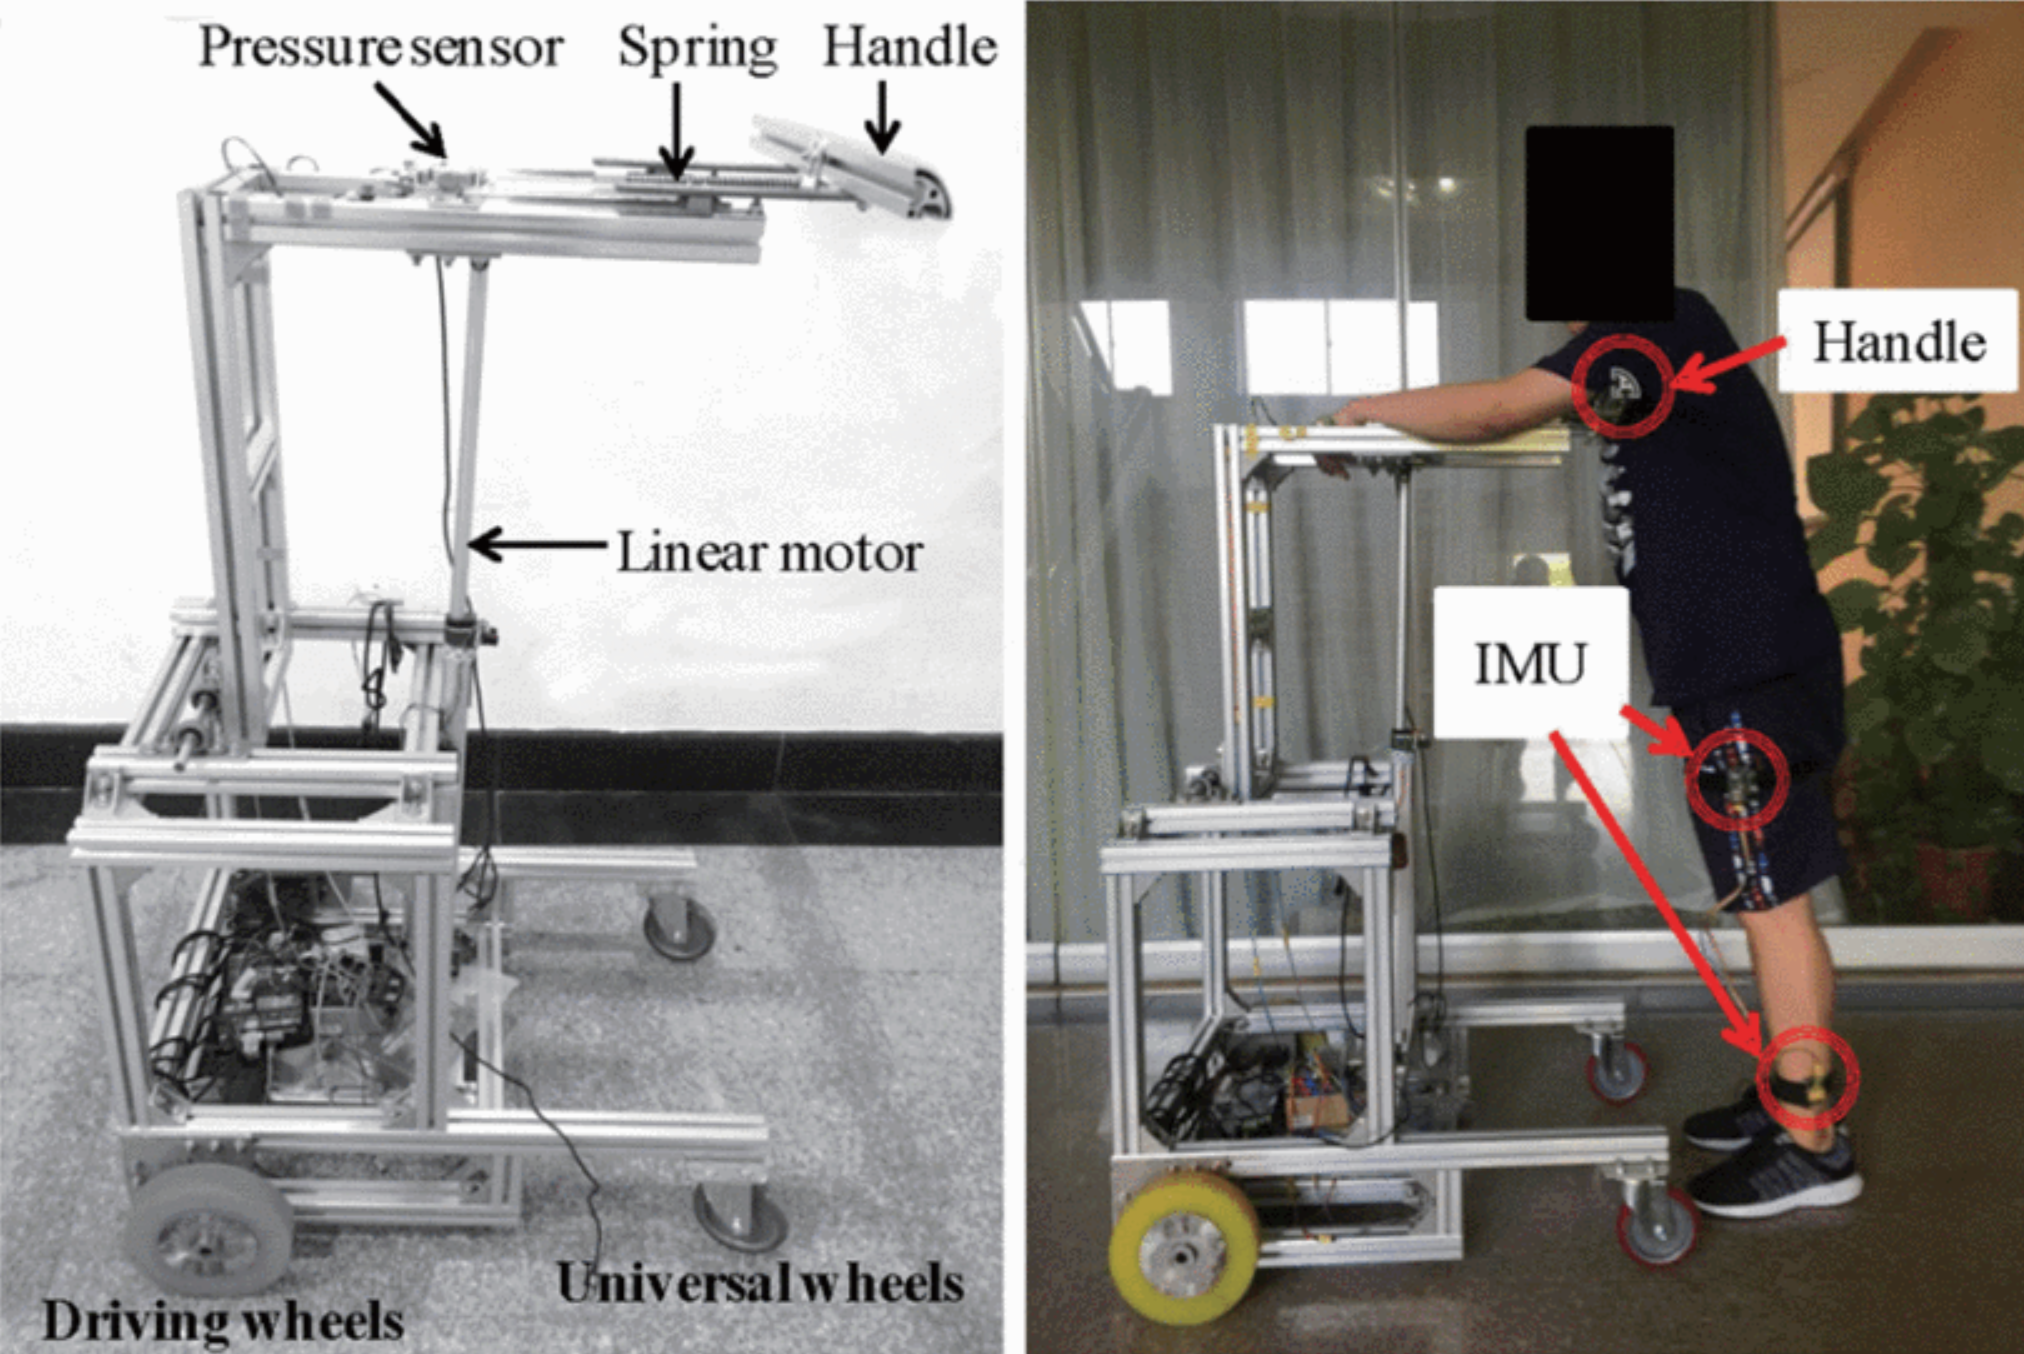
\includegraphics[width=\textwidth]{TESIS/imagenes/chap02/AplWalkerRobotic2.png}
\caption{ Andador robótico multifunción guiado por sensores de medición inercial y un modulo de transmisión de fuerza. \cite{walker8688067}}
\label{fig:robotic_walker}
\end{figure}

Un modulo de interfaz de usuario supervisa la progresión lineal en un grado de libertad utilizando sensores de medición. En base al principio bípedo, calcula el ángulo dinámico necesario para reflejar el movimiento cinemático, y así determinar las señales de control que serán enviadas a los controladores del motor. Finalmente, las señales recibidas son colocadas en un ciclo de retroalimentación que determinan los comandos del motor para controlar el andador robótico multifunción \cite{Modise2016}.

\section{Revisión Sistemática Basada en Evidencias} \label{fundamentos:RSBE}

Esta sección aborda el paradigma basado en evidencias, actualmente adoptado en muchas ciencias prácticas (i.e. medicina, educación, política social e ingeniaría). Las \gls{SLR} son un aspecto esencial del paradigma basado en evidencias, y tienen como objetivo sintetizar los estudios de investigación asociados a una pregunta de investigación específica, de forma rigurosa, auditable y justa. 

La presentación en cada subsección, describe el beneficio y el potencial de las revisiones sistemáticas de la literatura, razón por la cual será la metodología de investigación adoptada durante el proyecto PARKIBIP. Asimismo, procura especificar el flujo de actividades estándar a realizar en una SLR.

\subsection{Paradigma basado en evidencias}

Para lograr un mayor entendimiento se considera apropiado iniciar por el significado de \gls{evidencia} en un marco científico y tecnológico, ya que será aplicado a practicas de ingeniería de software en la realización de PARKIBIP.

En general, la evidencia se asocia al conocimiento. Normalmente se espera que el conocimiento se derive de la evidencia a través de algún proceso de interpretación (i.e. un modelo matemático o estadístico), y no basado en ilusiones. Por ejemplo, una ilustración menos científica ocurre cuando un jurado, en un juicio penal, tiene que considerar la evidencia de un conjunto de testigos para obtener un conocimiento razonable sobre lo sucedido. Asimismo, analizar dicho proceso por el cual se interpreta el primero para agregar o inferir el segundo es de suma importancia. Se detectan dos parámetros esenciales para producir evidencia solida a partir de un proceso de revisión objetiva: 

\begin{itemize}
    \item Selección objetiva e imparcial de estudios relevantes 
    \item Síntesis sistematizada de los resultados de los estudios previamente seleccionados
\end{itemize}

En resumen, la practica basada en evidencias (EBP, por sus siglas en ingles) busca utilizar un enfoque objetivo, riguroso y planificado para seleccionar estudios relevantes y realizar una sıntesis de los resultados de esos estudios \cite{Kitchenham2006}. La rigurosidad metodológica hace que los resultados sean mas confiables, ya que es posible estudiar el procedimiento llevado a cabo para su obtención ası como también reproducirlo.

La ingeniería de software basada en evidencias realiza un fuerte énfasis en el rigor metodológico involucrando los siguientes cinco pasos \cite{Kitchenham2004, Pizard}:

\begin{enumerate}
    \item Convertir un problema relevante o una necesidad de información en una pregunta que pueda ser respondida.
    \item Buscar en la literatura la mejor evidencia para responder a esa pregunta.
    \item Evaluar de forma crıtica la validez, el impacto y la aplicación de la evidencia.
    \item Integrar la evidencia evaluada con la experiencia practica y los valores y circunstancias de los interesados.
    \item Evaluar la efectividad y la eficiencia de este proceso para buscar maneras de mejorarlo.
\end{enumerate}

Los primeros tres pasos son esencialmente el papel de la revisión sistemática de literatura, mientras que el cuarto, es el de la traducción del conocimiento. El quinto es garantizar que los procedimientos de investigación estén sujetos a un análisis constante.

Para brindar una definición concisa a la técnica mencionada, es necesario clasificar las investigaciones en estudios:

\begin{itemize}
    \item Primarios: métodos utilizados para realizar estudios con el objetivo de obtener evidencia empírica sobre un tema de interés (i.e. encuestas, experimentos, estudios de caso, investigación y acción - del ingles, action research-).
    \item Secundarios: métodos que permiten recopilar de manera sistemática y rigurosa los estudios primarios relacionados con una pregunta de investigación específica, con el objetivo de sintetizar la evidencia disponible para responder a dicha pregunta (i.e.  revisión sistemática de literatura).
\end{itemize}

De esta manera, una revisión sistemática de literatura o SLR es un estudio secundario generado a partir de estudios primarios, y se define como un método para identificar, evaluar e interpretar todas las investigaciones pertinentes a una determinada pregunta de investigación, área, temática o fenómeno de interés. Es la principal herramienta del paradigma basado en evidencias, siendo sistemáticas -porque se conducen siguiendo un conjunto de procedimientos bien delineados y reproducibles-, además tratan de evitar sesgos, son rigurosas y abiertas.

La ilustración Fig. \ref{fig:context_srl} permite resumir mediante un esquema macro el flujo de información entrante y saliente relativo a una SLR; así como también el impacto futuro en políticas, estándares y practicas. 

\begin{figure}[H]
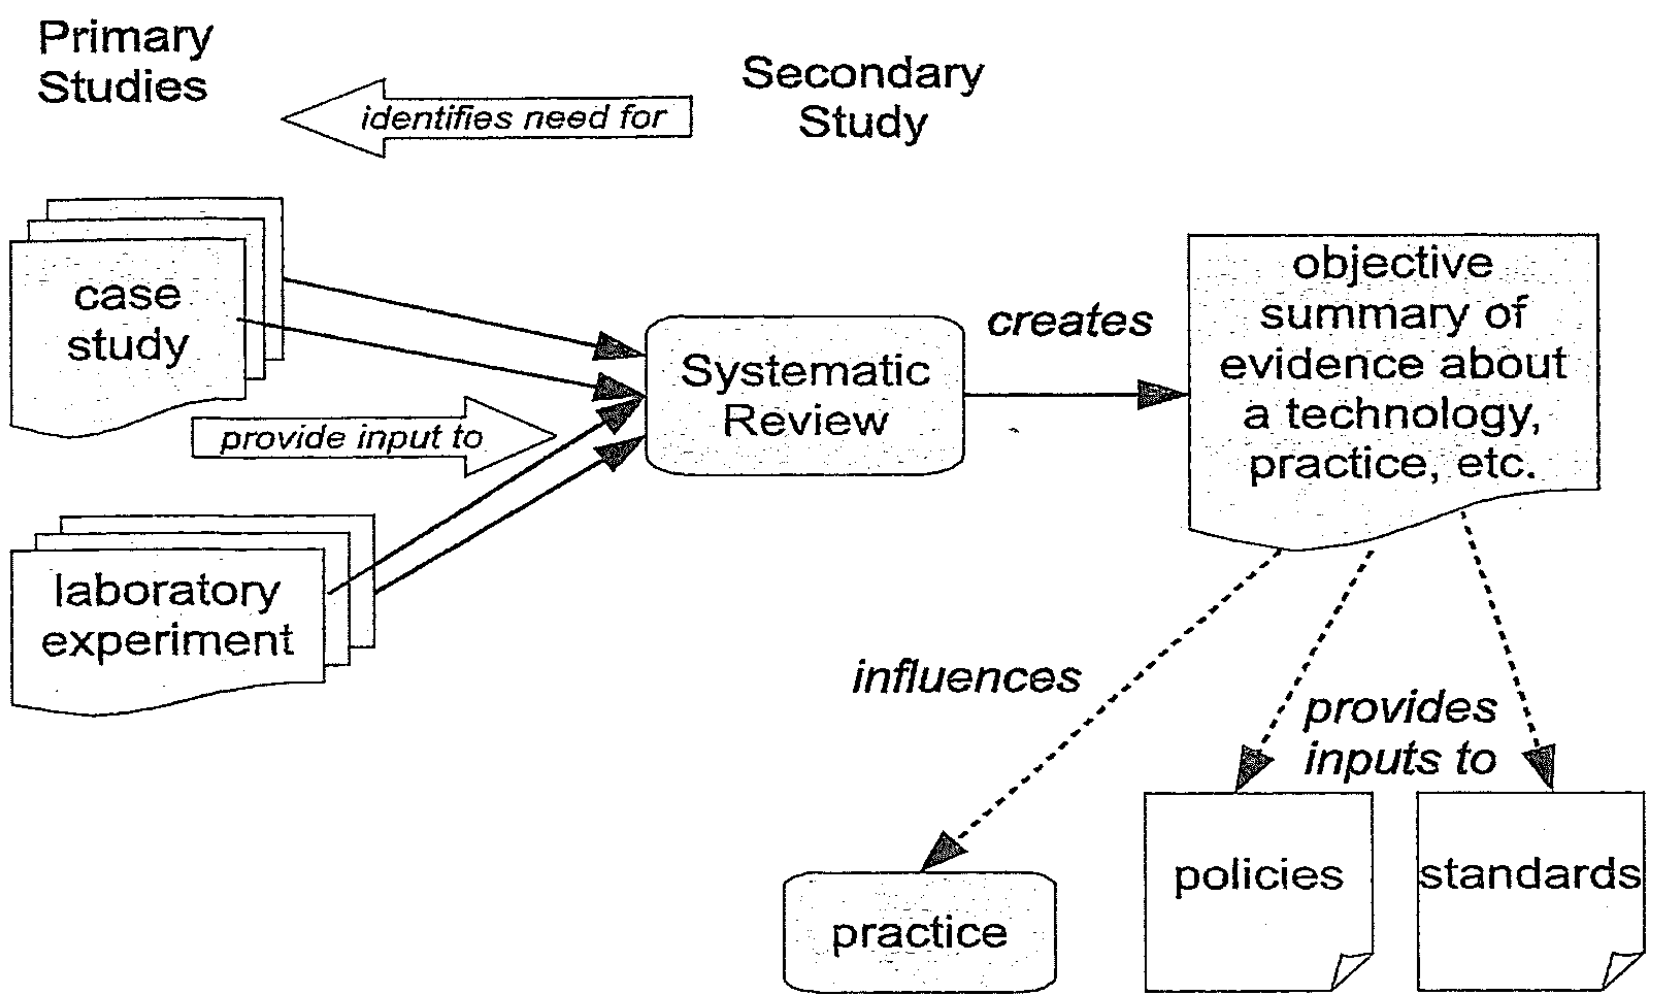
\includegraphics[width=\textwidth]{TESIS/imagenes/chap02/Contexto_RSL.PNG}
\caption{ Contexto de una revisión sistemática de literatura \cite{Kitchenham2006}.}
\label{fig:context_srl}
\end{figure}

\subsection{Revisión sistemática de literatura}

En general, los investigadores ejecutan las revisiones para resumir la evidencia científica existente sobre algún fenómeno particular, de manera exhaustiva e imparcial. Según una encuesta reciente, los principales factores de motivación en la ingeniería de software son:

\begin{itemize}
    \item Reunir conocimiento respecto a un campo o estudio en particular.
    \item Identificar recomendaciones para investigaciones futuras.
    \item Establecer el contexto de un tema o problema de estudio.
    \item Identificar las principales metodologías y técnicas de investigación usadas en un campo de investigación particular.
\end{itemize}

\noindent Realizar una revisión sistemática es un proceso extremadamente lento, que requiere suma atención en los detalles. Siempre es bueno comenzar por establecer la necesidad (i.e. ya existe otra que aborde el mismo tema) y por ende la motivación de ejecutar una revisión, para luego evaluar su factibilidad. 

Asimismo, especificar los aspectos técnicos del proceso de revisión (planeamiento) es un factor fundamental para lograr resultados satisfactorios. Esto es, desarrollar un protocolo de revisión que permita realizar y documentar las estrategias y toma de decisiones de diseño del estudio. Su definición de antemano puede ayudar a reducir la probabilidad de sesgo, limitando la influencia de las expectativas del investigador (i.e. la selección de estudios primarios o la síntesis de los resultados). A modo de ejemplo se propone la Tabla \ref{tab_protocolcomponents},que sugiere los componentes a incluir en un protocolo de revisión.
\begin{table}[H]
    \begin{center}
     \caption{\label{tab_protocolcomponents} Componentes de un protocolo de revisión}
        \begin{tabular}{ |p{12cm}| } 
        \hline
        Antecedentes y justificación de la revisión. \\
        \hline
        Preguntas de investigación.\\
        \hline
        Estrategia de búsqueda para estudios primarios. Debe incluir los términos de búsqueda y recursos donde se realizar´a la búsqueda. Los recursos incluyen librerıas digitales, revistas especıficas, y actas de congresos.\\
        \hline
        Criterios de selección de estudios. Usados para determinar cuales estudios son incluidos o excluidos de la revisión sistemática.\\
        \hline
        Procedimientos de selección de estudios. El protocolo debe describir como se aplicar´a el criterio de selección, por ejemplo, cuantos asesores evaluaran cada estudio primario, y como se resolverán los desacuerdos entre los evaluadores.\\
        \hline
        Procedimientos y listas de verificación para evaluar la calidad.\\
        \hline
        Estrategia de extracción de datos.\\
        \hline
        Método o técnica de sıntesis de los datos.\\
        \hline
        Limitaciones.\\
        \hline
        Estrategia de difusión.\\
        \hline
        Calendario del proyecto de revisión.\\
        \hline
        \end{tabular}
    \end{center}
\end{table}

\noindent Dentro de la fase de planeamiento, otro ítem sumamente determinante, es establecer las preguntas de investigación que guiarán e incidirán en todo el estudio (i.e. que estudios primarios incluir o excluir, decidir que datos deben extraerse y cómo sintetizar los datos para contestar las preguntas). Una pregunta es adecuada cuando \cite{Kitchenham2004}:

\begin{itemize}
    \item Es significativa e importante tanto para investigadores como para profesionales.
    \item Dará lugar a cambios o incrementará la confianza en las practicas actuales de la ingenierıa de software.
    \item Identificará las discrepancias entre las creencias comúnmente aceptadas versus la realidad.
\end{itemize}

Posterior a la etapa de diseño o planeamiento, inicia la fase de ejecución de la revisión sistemática. Si bien no será objeto de aplicación en el proyecto PARKIBIP, y por lo tanto no será analizada con detenimiento, es importante mencionar la última etapa de Documentación y publicación del estudio. El esquema en la figura Fig. \ref{fig:review_phases} expone un patrón organizado y sistemático a seguir en la realización de una SLR. De igual manera, incluye la clasificación en fases y el protocolo de revisión mencionados anteriormente.

\begin{figure}[h!]
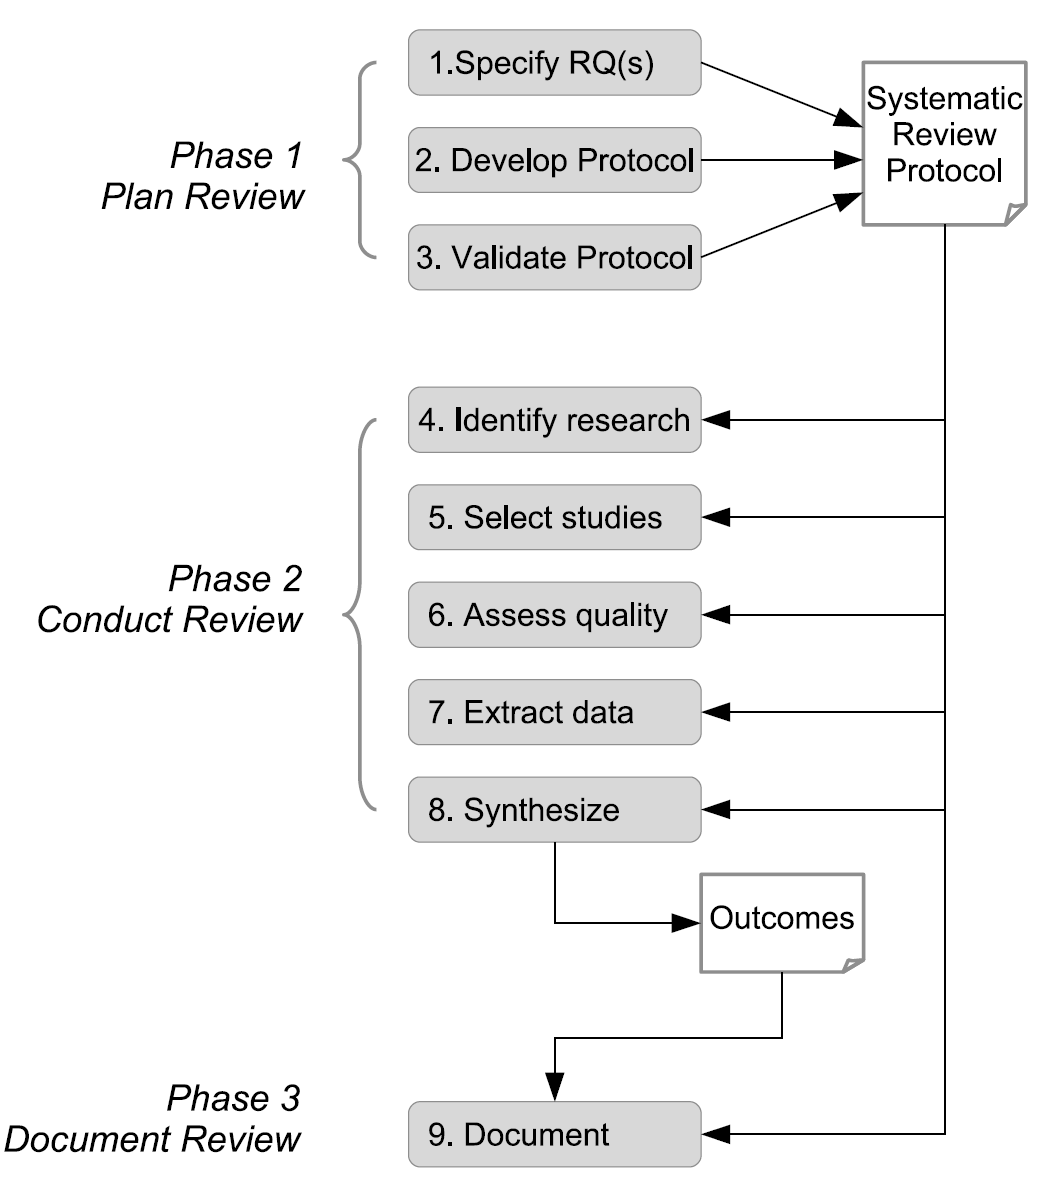
\includegraphics[width=\textwidth]{TESIS/imagenes/chap02/review_phases.PNG}
\caption{Flujo de actividades en el proceso de una SLR. \cite{Kitchenham2006}}\label{fig:review_phases}
\end{figure}

En resumen, una SLR tiene ciertas etapas discretas contempladas en tres fases principales, cada una con sus actividades particulares:
\begin{enumerate}
    \item Planificar la Revisión 
    \begin{itemize}
        \item Especificar las preguntas de investigación.
        \item Desarrollar el protocolo de revisión.
        \item Evaluar el protocolo de revisión (recomendada).
    \end{itemize}
    \item Realizar la Revisión
    \begin{itemize}
        \item Identificar la investigación.
        \item Seleccionar los estudios primarios.
        \item Evaluar la calidad de los estudios.
        \item Extraer datos y monitorear.
        \item Sintetizar los datos.
    \end{itemize}
    \item Informar la Revisión
    \begin{itemize}
        \item Especificar los mecanismos de difusión.
        \item Formatear el informe principal.
        \item Evaluar el informe (recomendada).
    \end{itemize}
\end{enumerate}

Es relevante notar, que la lista de fases de una revisión sistemática es una guía sugerida y bien estructurada. Además, no es estrictamente secuencial y algunas pueden repetirse mas de una vez, involucrar iteraciones o de ser necesario volver a ejecutar etapas. En otras palabras, el proceso podrá tener variaciones al caso típico y dependerá exclusivamente del contexto de aplicación, las necesidades y las limitaciones del proyecto, así como también las decisiones de los revisores.

A continuación, se hará una breve introducción a las principales actividades de la fase ``Realizar una revisión sistemática''. Comprender el propósito y aplicación de cada sub-etapa, será sustancial para acompañar con éxito el desarrollo de la metodología en el proyecto PARKIBIP -Cap. \nameref{chap_RSBE}-. 

\begin{enumerate}[label=(\roman*)] 
\item Identificar la investigación. En esta etapa se establece y utiliza una estrategia de búsqueda para obtener una lista de todas las publicaciones relevantes para las preguntas de investigación. La estrategia de búsqueda puede ser automatizada mediante librerías digitales, búsquedas manuales, o mediante contactos con los investigadores; pero tiene que estar definida en el protocolo de la revisión y debe ser reportada luego de forma transparente y replicable. Una alternativa de búsqueda -a veces utilizada como complemento-, es el uso de las referencias en la búsqueda de nuevos estudios. Iniciando desde un estudio primario de interés, para luego emplear sus referencias para encontrar nuevos estudios relevantes (\gls{backward_snowballing}) o se buscan cuales estudios lo ubican en sus referencias (\gls{forward_snowballing}). En caso de utilizar una búsqueda automatizada, se debe incluir una descripción de la cadena de búsqueda y los recursos utilizados.
  \item Seleccionar los estudios primarios. En este paso se establecen los criterios de selección de artículos primarios, que determinarán aquellas publicaciones que serán incluidas -Crit. Inclusión, definen qué estudios se deben incluir como relevantes- o excluidas -Crit. Exclusión, se aplican sobre los estudios seleccionados o sobre la lista inicial para remover estudios irrelevantes- de la revisión. Los criterios de selección pretenden identificar los estudios primarios que proporcionan evidencia directa acerca de las preguntas de investigación. Según el procedimiento estipulado, el procedimiento de selección de artículos puede basarse en la lectura rápida de la combinación titulo, resumen, palabras claves de las publicaciones primarias -en general, se tienen muchos artículos, y es imposible leerlos por completo-.
  \item Evaluación de calidad. Evaluar la calidad de un articulo es una actividad desafiante, y conlleva a establecer qué parámetros de calidad serán evaluados y el procedimiento para su aplicación. En general es adecuado definir un lista de chequeos (del ingles, checklist) en base a preguntas concisas y proceder a aplicarlos de tal forma que asegure la mejor calidad de la evaluación. La calidad se refiere a la medida en que el estudio minimiza el sesgo y maximiza tanto la validez interna como la externa.
  \item Extracción de datos. El objetivo de esta etapa es el diseño de formularios de extracción de datos para que los investigadores puedan registrar adecuadamente la información que se obtiene de los estudios primarios. El formulario deberıa incluir información asociada a la extracción, información general del estudio,(i.e. identificador del estudio, titulo y detalles de publicación), preguntas que habiliten a responder las preguntas de investigación, preguntas para evaluar la calidad de los estudios y resumen de los datos.
  \item Síntesis de datos. La síntesis es el proceso en el cual se recolectan, integran y resumen los hallazgos incluidos en los estudios primarios. Sin importar el tipo de síntesis -descriptiva (o narrativa) y cuantitativa-, se debería comenzar con la creación de un resumen de los estudios incluidos, presentando intervenciones, numero y característica de los participantes, resultados, entre otros. Una alternativa es realizar una síntesis temática y narrativa, en donde los datos se presentan tabulados, de tal forma que sean consistente con las preguntas de investigación. Es relevante notar, que el resultado de la síntesis es el disparador para las conclusiones finales.
\end{enumerate}

\section{Análisis de la marcha}

En los últimos años, el análisis de la marcha y la partición de sus fases ha sido un tema de investigación desafiante debido a su impacto en muchas aplicaciones relacionadas con tecnologías de la marcha. El paso o la marcha humana es un proceso complejo y cíclico que requiere la sinergia de los músculos del cuerpo, los huesos y el sistema nervioso \cite{SAUNDERS1953}, principalmente dirigido a mantener la posición vertical y mantener el equilibrio durante condiciones estáticas y dinámicas \cite{Ayyappa1997}. 

El análisis de la marcha o \gls{gait_analysis} instrumentado provee mediciones confiables y objetivas sobre los patrones de locomoción y su variabilidad. Estas mediciones, pueden contribuir a la investigación de patologías y definición de programas de rehabilitación. GA está emergiendo como una herramienta efectiva para detectar enfermedades neurodegenerativas o para monitorear su progresión \cite{Bertoli2018}. Específicamente, los parámetros de la marcha son indicadores útiles para discriminar enfermos de Parkinson así como para cuantificar la severidad de la enfermedad. Aprovechando los modelos cinemáticos, los sistemas pueden identificar ciertos patrones en las señales para detectar pasos y calcular parámetros; como la cadencia, la longitud de zancada, la velocidad de zancada, el rango de movimiento, los ángulos de las articulaciones, la velocidad máxima de oscilación, sentarse para pararse y pararse para sentarse, tiempos de transición, tiempo de giro, velocidad máxima de giro, etc. Estos parámetros han mostrado una correlación significativa con el diagnóstico de la enfermedad de Parkinson y la cuantificación de su severidad \cite{Akbari2017}.

\subsection{Identificación de fases de la marcha}

El ciclo de la marcha se define como el período de tiempo que transcurre desde el contacto inicial de un pie con el piso, hasta la próxima ocurrencia del mismo evento en el mismo pie. Existen muchos modelos de partición de dicho ciclo, con diferentes niveles de granularidad, que dependen de los objetivos clínicos: el modelo que incluye dos grandes fases de la marcha, es decir, apoyo y vuelo, es en general el más adoptado según la revisión sistemática de \cite{Taborri2016}; la cual recopila una gran variedad de estudios dentro del GA así como los distintos modelos empleados para distinguir el ciclo de la marcha en sus respectivas fases. La siguiente figura Fig. \ref{fig:gait-phases}, condensa los distintos hallazgos y nomenclaturas empleadas en la literatura respecto a las granularidades del ciclo de la marcha.

\begin{figure}[H]
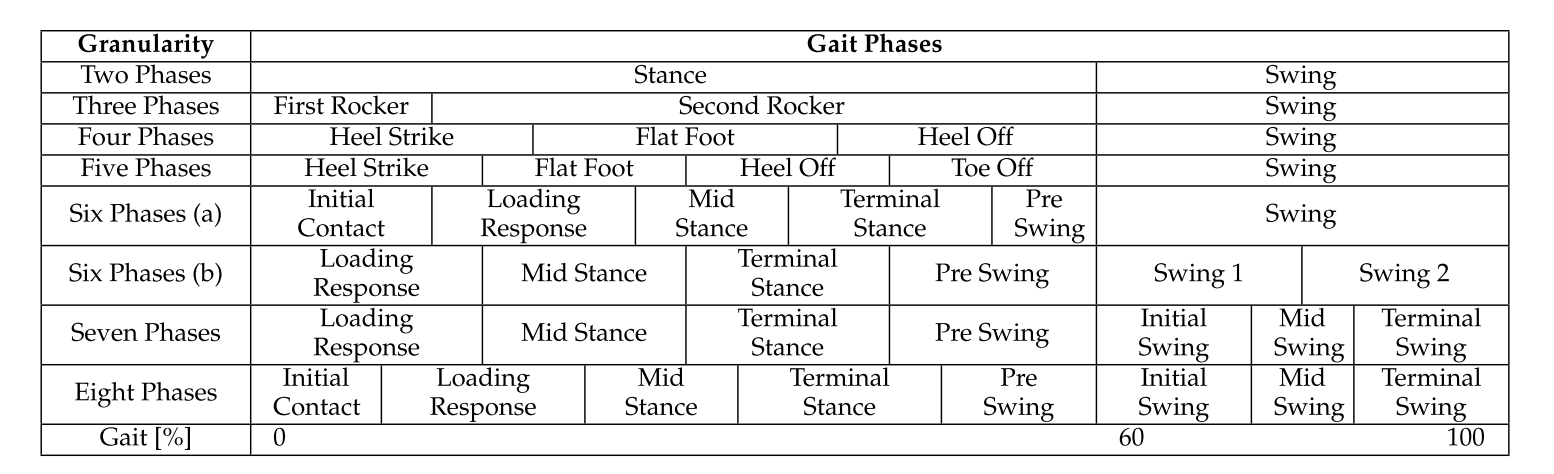
\includegraphics[width=\textwidth]{TESIS/imagenes/chap02/Gait-phases-classification.png}
\caption{ Nomenclatura para diferentes granuralidades del ciclo de marcha \cite{Taborri2016}.}
\label{fig:gait-phases}
\end{figure}

La correcta discriminación de las fases de la marcha es considerado un punto de partida para muchas aplicaciones, por ejemplo: (i) la evaluación del estado de recuperación de la marcha durante tratamientos de rehabilitación o luego de alguna intervención; (ii) la clasificación de las distintas actividades de la vida diaria o AVD; (iii) el control sinérgico de los dispositivos robóticos, para la recuperación de la movilidad de las extremidades inferiores; (iv) el entrenamiento atleta; y finalmente, (v) para distinguir una marcha normal de una patológica \cite{Taborri2016}.

\subsection{Sensores de medición para análisis de la marcha}

Una variedad de sensores pueden ser utilizados para alimentar algoritmos que identifican las distintas fases de la marcha, clasificados principalmente como vestibles o no vestibles - del ingles \gls{Wearables} y \gls{non_Wearables} respectivamente- . Dentro de los sensores vestibles, las plantillas de presión (en inglés ``footswitches'') son consideradas un estándar  \cite{Taborri2016}; sin embargo, para resolver algunas limitaciones inherentes en estos dispositivos, las unidades de medición inercial se han vuelto muy populares en la última década. Buenos resultados han sido alcanzados utilizando también sensores de ultrasonido, electro-miografías (EMG) y electro-neurografías (ENN). 

Los sensores no vestibles, como los sistemas optoelectrónicos o las plataformas de fuerza, se mantienen como los sistemas más precisos para analizar la marcha en ambientes interiores. A pesar de su utilidad, han tenido un uso muy limitado, especialmente en países en desarrollo, debido al alto costo que implica establecer un laboratorio especializado de marcha. La principal desventaja de este tipo de sistemas, es que no proveen una evaluación de los pacientes durante sus actividades cotidianas, extrapolando las conclusiones de un estudio de corto tiempo que no refleja las condiciones reales del paciente. Además, la evaluación puede requerir mucho tiempo y puede ser difícil de tolerar por los sujetos, principalmente si se trata de condiciones patológicas \cite{Kumar8372660}.

Resulta fundamental para el proyecto PARKIBIP identificar el tipo apropiado de sensor que se utilizará para nutrir los algoritmos, que luego detectarán las distintas fases de la marcha en tiempo real. Es inherente al objetivo del proyecto que el tipo de sensor debe ser del tipo vestible o wearable, ya que el sistema debe ser portable y utilizable en ambientes exteriores. Una revisión sistemática basada en evidencias del año 2016 \cite{Taborri2016} identifica, selecciona y categoriza las distintas metodologías utilizadas para la detección de fases de la marcha, analizando ventajas y desventajas de cada una de las soluciones. 

Los pedales (en inglés, ``footswitches'') son dispositivos que emplean sensores capaces de detectar el contacto del pie con el piso durante un ciclo de marcha. Se emplean principalmente para medir parámetros temporales en la marcha. Estos sensores, que van colocados en la parte inferior del pie, operan como interruptores y se encuentran conectados por cables a algún tipo de terminal. Al ser de bajo costo y proveer una precisión muy alta, son usualmente utilizados para complementar la medición de otro tipo de sistema. Sin embargo, presentan varias desventajas claves para PARKIBIP, como por ejemplo: (i) el número de fases detectables es limitado, dado que las sub fases en la etapa de vuelo del pie no pueden ser discriminadas; (ii) el lugar en el que son dispuestos los sensores, en los pacientes con marcha patológica, afecta la precisión y la confiabilidad de medición \cite{AMINIAN2002689}; por ultimo, (iii) la conexión cableada afecta la oportunidad del sistema de ser un instrumento para las actividades de la vida diaria de los sujetos afectados.

Las plantillas de presión o ``Foot Pressure Insoles'', presentan ventajas y desventajas similares a los pedales, ya que se basan en los mismos principios. Si bien existen plantillas que no requieren cableado, por ende no presentan dicha desventaja, éstas son de un costo elevado en comparación a los pedales u otras soluciones (p. ej. los sensores de aceleración, giroscopios o incluso las unidades de medición inercial). 

El acelerómetro es la solución más utilizada para el análisis del paso ambulatorio. Con el objetivo de reconocer las fases del paso de un individuo, la evidencia literaria existente describe diferentes combinaciones de éstos sensores, junto a los posibles lugares donde pueden ser ubicados. Los acelerómetros, entre otras unidades inerciales, son relativamente pequeños, de baja energía y larga autonomía, baratos, portables y altamente accesibles en la industria \cite{TongKaiyuGranat1999}. En comparación con las soluciones basadas en pedales o plantillas ya mencionadas, el análisis de la aceleración ha permitido a los investigadores distinguir ciertas fases de la marcha, como lo es la sub-fase de etapa de vuelo (o en ingles, fase de Swing). Sin embargo, el empleo de acelerómetros para identificar las fases de la marcha, implica ciertas complejidades que resultan críticas: (i) la necesidad de compensar la gravedad durante el cómputo de la aceleración, de la parte del cuerpo analizada; (ii) el error acumulado en la integral doble aplicada al conjunto de datos sensados, para el cálculo de la posición; y, (iii) el procedimiento de calibración que permite ubicar de forma correcta el sensor respecto a un estándar de referencia trazable, y así confiar en la validez de sus mediciones.

La velocidad angular -como una variable para la partición de las fases del paso-, dato extraído desde el dispositivo giroscopio, ha adquirido una gran popularidad en las últimas décadas y es preferida sobre otras variables inerciales. La velocidad angular no se encuentra afectada por la gravedad, como tampoco la curva de sus ondas por el toque del talón con el suelo (a.k.a. ``heel strike''). Además, no es necesario mantener un cuidado minucioso respecto a la posición en donde es ubicado el giroscopio dentro del segmento del cuerpo a medir. Aunque, una desventaja en su utilización es que, tal como la aceleración, la velocidad angular también se ve alterada por el error propagado, en caso de que se compute el ángulo del movimiento. 

\subsection{Unidad de Medición Inercial (IMU)}

La Unidad de Medición Inercial, también conocida como IMU (Inertial Measurement Unit, por sus siglas en inglés), combina varios de los sensores mencionados, como por ejemplo el acelerómetro y el giroscopio; algunos también incluyen magnetómetro, barómetro, sensores de luz y/o temperatura, entre otros. 

Por su parte, los dispositivos IMUs presentan una serie de ventajas que hace con que sea el tipo de dispositivo adecuado para el proyecto PARKIBIP. A continuación, se listan algunas de ellas \cite{ZAGO201844}:

\begin{itemize}
    \item La combinación de diferentes cantidades inerciales permite la evaluación de diferentes tipos de primer contacto con el piso, el cual representa un índice sumamente importante para analizar el estado de salud del sujeto, utilizando la estimación de la orientación del pie. 
    \item La fusión de los datos de velocidad angular y aceleración lineal permiten compensar el error acumulado. 
    \item Estos dispositivos permiten la evaluación en tiempo real de los parámetros espacio-temporales en entornos de la vida real, interiores y exteriores, superando así las limitaciones típicas de las mediciones de laboratorio.
    \item Los IMUs son más baratos y más prácticas que los sistemas de GA completos; solo se requiere una preparación relativamente rápida de los pacientes, ya que el sensor se coloca en el cuerpo por medio de un cinturón elástico.
    \item Los datos se pueden transferir fácilmente a través de Bluetooth al software dedicado.
\end{itemize}

Si bien el dispositivo tiene un gran potencial para el proyecto PARKIBIP, se deberán tener en cuenta ciertos factores que pueden afectar la señal de entrada y salida \cite{Anwary8246577}. Por ejemplo, durante la caminata, el movimiento de la ropa puede causar interferencias con la salida del acelerómetro. Puede haber vibración o ruido causado por el impulso si el sensor no es ajustado correctamente. Ajustar el sensor en un cinturón o cargarlo en el bolsillo también puede inducir interferencia de movimiento relativo. Para aumentar la confiabilidad y validez de la extracción automática de los parámetros para el análisis de la marcha, es fundamental elegir correctamente el lugar donde serán colocados los sensores y la forma en la que se coloquen.  % Se carga el capítulo Fundamentos o antecedentes
  \chapter{Revisión sistemática basada en evidencia}\label{chap_RSBE}

En este proyecto se realizó una revisión sistemática basada en evidencia científica relacionada al uso de sensores IMU para analizar la marcha de las personas al caminar. Conforme a los requerimientos del proyecto, el objetivo de la revisión sistemática se centró en identificar todo el material relevante que permita estudiar la marcha de las personas con el uso de sensores, reducir o eliminar incertidumbres en la investigación, y sobre todo no reinventar la rueda. El conocimiento recopilado fue fundamental para la implementación de la solución PARKIBIP, para mejorar la marcha de los pacientes con la enfermedad de Parkinson.

\section{Planeamiento y diseño de Protocolo de Revisión}

Es esencial para alcanzar resultados satisfactorios establecer un plan, llamado protocolo de revisión, con todas las actividades a realizar y criterios a utilizar previo a la ejecución de la SLR. Desarrollar dicho plan, permite guiar y registrar las estrategias y toma de decisiones de diseño del estudio (es decir, es el documento de referencia).

A su vez, la actividad de planeación incluye definir las preguntas de investigación y desarrollar la estrategia de búsqueda, los criterios de inclusión/exclusión, el formulario de extracción de datos, ente otros.

De esta manera, a través de un proceso iterativo y mediante la participación activa de todos los miembros del equipo en el desarrollo, se estableció un protocolo de revisión en una hoja de cálculos tabulada. Resultó esencial para su construcción la realización de diversas pruebas piloto con el mismo que permitan encontrar inconsistencias en los procedimientos de recolección y agregación de los datos. 

Para establecer el objetivo de la revisión sistemática, se plantean cuatro preguntas de investigación que guían la revisión:

\begin{itemize}
    \item ¿Qué tipo de sensores IMU se utilizan para medir la marcha de las personas?
    \item ¿Cuántos sensores son necesarios para medir las características de la marcha?
    \item ¿Qué datos sobre la marcha se pueden obtener con los distintos sensores?
    \item ¿Qué técnicas o algoritmos se utilizan para analizar y procesar los datos?
\end{itemize}

La tabla Tab. \ref{tab_protocolcomponents_PARKIBIP} resume los componentes del protocolo, especifica los métodos que se utilizarán para llevar a cabo la SLR; su definición de antemano ayuda a reducir la probabilidad de sesgo en la investigación. 

\begin{longtable}[p{15cm}]{|p{5cm}|p{10cm}|}
\hline
\multicolumn{2}{| c |} {\textbf{1. Contexto}}  \\ \hline
\textbf{1.1. Objetivo} & Investigar el uso de sensores IMU para analizar la marcha de las personas al caminar\\\hline
\textbf{1.2. Necesidad} & Se quiere mejorar la marcha de las personas con enfermedad de Parkinson, por lo que se quiere relevar la forma de estudiar la marcha de las personas con el uso de sensores\\ \hline
\textbf{1.3. Preguntas de investigación} & \\ \hline
RQ1 & Qué tipo de sensores IMU se utilizan para medir la marcha de las personas?\\ \hline
RQ1.1 & Cuántos sensores son necesarios para medir la marcha? \\ \hline
RQ1.2 & Qué datos sobre la marcha se pueden obtener con los distintos sensores?\\ \hline
RQ1.3 & Qué técnicas o algoritmos se utilizan para analizar y procesar los datos?\\ \hline
%Start Search strategy 
 \multicolumn{2}{| c |}{\textbf{2. Proceso de Búsqueda}}\\ \hline
\textbf{2.1. Estrategia} & Búsqueda automática en título, abstract y keyworkds filtrado por diciplina\\ \hline
\textbf{2.2. Snowballing} & No\\ \hline
\textbf{2.3. Términos} & \\ \hline
Gait analysis & Gait analysis, step analysis, step detection, gait detection\\ \hline
Inertial measurement unit & IMU, Inertial measurement unit\\ \hline
Foot-ground contact & Foot-ground contact, foot ground detection, FGCD\\ \hline
\textbf{2.4. Cadena de Búsqueda} & TITLE-ABS-KEY ( ( ``gait analysis''  OR  ``step analysis''  OR  ``step detection''  OR  ``gait detection'')  AND  ( ``imu''  OR  ``inertial measurement unit'' )  OR  ( ``foot ground contact''  OR  ``foot-ground contact''  OR  ``foot ground detection''  OR  ``FGCD'' ) )  AND  PUBYEAR  $>$  2015  AND  ( LIMIT-TO ( SUBJAREA ,  ``ENGI'' )  OR  LIMIT-TO ( SUBJAREA ,  ``COMP'' )  OR  LIMIT-TO ( SUBJAREA ,  ``BIOC'' )  OR  LIMIT-TO ( SUBJAREA ,  ``MEDI'' ) )\\ \hline
\textbf{2.5. Motores y Cadenas de Búsqueda} & Portal Timbó, Scopus, ScienceDirect\\ \hline
\textbf{2.6. Fuentes a considerar} & N/A\\ \hline
\textbf{2.7. Período a tener en cuenta} & Debido a la evolución de las tecnologías, sensores y aplicaciones se consideran solamente los artículos con año de publicación 2016-2019\\ \hline
\textbf{2.8. Procedimientos auxiliares} & N/A\\ \hline
\textbf{2.9. Evaluación del Proceso de Búsqueda} & Muy bueno. Se logro obtener un numero adecuado de artículos seleccionados con posible buen aporte.\\ \hline
%Start selection process
 \multicolumn{2}{| c |}{\textbf{3. Proceso de Selección de Estudios Primarios}}\\ \hline
\textbf{3.1. Criterios de Inclusión} & Que sea completo. Que se tenga acceso al artículo. Estudios en Ingles, Español y Portugués. Año de publicación $>$ a 2015.\\ \hline
\textbf{3.2. Criterios de Exclusión} & Que no sean papers científicos o con el formato incorrecto. Que no traten la marcha de personas. Que usen sensores difíciles de acceder. Descartar estudios duplicados. Que usen sensores que no sean IMU. Que se enfoquen en la posición en la que se encuentra el sujeto y no en los parámetros de la marcha\\ \hline
\textbf{3.3. Roles de los revisores} & Ambos revisores realizarán las mismas tareas de forma equitativa. Selección, extracción y síntesis.\\ \hline
\textbf{3.4. Cómo se evaluará el acuerdo entre revisores} & Coeficiente de acuerdo Kappa\\ \hline
\textbf{3.5. Cómo se resolverán diferencias} & Discusión abierta en busca de un acuerdo. En caso de no llegar al acuerdo sera excluido.\\ \hline
\multicolumn{2}{| c |}{\textbf{4. Proceso de Evaluación de la Calidad de los Estudios}}\\ \hline
\textbf{4.1. Se evaluará la calidad de los estudios (justificar)} & Si. \\ \hline
\textbf{4.2. Lista de Verificación propuesta (del ingles, Checklist)} & En esta etapa se utilizará la técnica de evaluación Scoring, la cual consiste en plantear una checklist y asignarle a cada ítem el valor 0 ó 1. Luego, se suma el puntaje obtenido para la checklist y se discute la exclusión del articulo.\\ \hline
\textbf{4.3. Cómo se evaluará el acuerdo entre revisores} & N/A\\ \hline
\textbf{4.4. Cómo se resolverán diferencias} & Discusión abierta en busca de un acuerdo. En caso de no llegar al acuerdo el articulo será excluido.\\ \hline
\multicolumn{2}{| c |}{\textbf{5. Proceso de Extracción de Datos}}\\ \hline
\textbf{5.1. Formulario de extracción} & Se establece un formulario en formato tabular que indica los campos de interés que direccionan las preguntas de investigación.\\ \hline
\textbf{5.2. Estrategia de extracción} & División equitativa de artículos. Revisiones de a pares en base a 1 articulo aleatorio.\\ \hline
\textbf{5.3. Consideraciones adicionales (datos calculados, subjetivos, etc.)} & El proceso sera proactivo y abierto a la inclusión de características que se consideren relevantes. Además, se pretende obtener un listado de tipos y/o marcas de los IMU, para luego realizar una comparación.\\ \hline
\multicolumn{2}{| c |}{\textbf{6. Proceso de Síntesis de Datos}}\\ \hline
\textbf{6.1. Tipo de Síntesis} & Se realiza una síntesis temática.\\ \hline
\textbf{6.2. Forma de validación de la síntesis} & N/A\\ \hline
\caption{\label{tab_protocolcomponents_PARKIBIP} Componentes del protocolo de revisión de PARKIBIP.}
\end{longtable}

\noindent Tal como se puede apreciar en la tabla, la misma se encuentra segmentada en distintas etapas, siendo consistente con las principales etapas de una SLR estándar.

\section{Estrategia de búsqueda}

Se planeó una estrategia de búsqueda automatizada, en función de la definición de una cadena de búsqueda que incluya la combinación de las palabras claves del problema de estudio, así como también sus alias (p. ej. Gait Analysis, IMU, etc.). Para ello, se seleccionaron los servicios de indexamiento y librerías digitales a través de portal Timbó (e.g, Scopus, IEEE, Springer Link), como motores de búsqueda principales.

Los términos de búsqueda utilizados se construyeron siguiendo los siguientes pasos:
\begin{enumerate}
    \item Definir los términos principales
    \item Identificar ortografías alternativas, sinónimos o términos relacionados para términos principales
    \item Verificar las palabras claves en los documentos relevantes previamente identificados
    \item Se usa el OR booleano para incorporar ortografías alternativas, sinónimos o términos relacionados
    \item Se usa el booleano AND para vincular los términos principales
\end{enumerate}


Es de gran importancia resaltar la codificación de la Cadena de búsqueda, la cual es imprescindible para ejecutar una búsqueda automatizada, y que de su buena formación dependerán los resultados futuros (i.e. una malformación de la cadena de búsqueda podrá alcanzar estudios irrelevantes, demasiados o una poca cantidad de los mismos). 
\newline
\noindent\fbox{
     \parbox{\textwidth}{
    \textit{
    TITLE-ABS-KEY ( ( ``gait analysis''  OR  ``step analysis''  OR  ``step detection''  OR  ``gait detection'')  AND  ( ``imu''  OR  ``inertial measurement unit'' )  OR  ( ``foot ground contact''  OR  ``foot-ground contact''  OR  ``foot ground detection''  OR  ``FGCD'' ) )  AND  PUBYEAR  $>$  2015  AND  ( LIMIT-TO ( SUBJAREA ,  ``ENGI'' )  OR  LIMIT-TO ( SUBJAREA ,  ``COMP'' )  OR  LIMIT-TO ( SUBJAREA ,  ``BIOC'' )  OR  LIMIT-TO ( SUBJAREA ,  ``MEDI'' ) )}
    }
}

\section{Criterios de inclusión/exclusión}

Se formularon criterios de selección de artículos a incluir en la revisión, con el fin de identificar aquellos estudios que proporcionen información relevante a las preguntas de investigación y eliminar estudios arbitrarios. Dichos criterios fueron expresados como dos conjuntos, criterios de inclusión y de exclusión, ilustrados en la Tabla \ref{TAB: criterios}.


\begin{table}[H] 
\caption{Criterios de selección de estudios primarios}
\centering
\hspace*{-1cm}%
\begin{tabular}{|p{7cm}|p{8cm}|}
\hline
\textbf{Criterios de inclusión} & \textbf{Criterios de exclusión}\\ \hline
Estudios completos & Estudios arbitrarios -no científicos- o con el formato incorrecto\\ \hline
Con acceso al artículo completo & No traten la marcha de personas\\ \hline
Escritos en los idiomas inglés, español y portugués  & Usen sensores que no sean IMU o difíciles de acceder\\ \hline
Publicados a partir del año 2015 & Se descartan estudios duplicados\\ \hline
    & Se enfoquen en la posición en la que se encuentra el sujeto y no en los parámetros de la marcha \\\hline
\end{tabular}
\hspace*{-1cm}
\label{TAB: criterios}
\end{table}

Asimismo, a través de la cadena de búsqueda se limitan aquellos estudios pertenecientes a las áreas de conocimiento Ingeniería, y/o Computación, y/o Medicina, y/o Bio-ciencias.

\section{Selección}

El propósito de esta etapa es recopilar estudios primarios que proporcionan evidencia directa acerca de las preguntas de investigación.
En primera instancia, los resultados primarios obtenidos fueron evaluados utilizando el título y el resumen del estudio para excluir aquellos que son claramente irrelevantes. Los documentos marginales o para los cuales la inclusión/exclusión es incierta, fueron mantenidos en el conjunto selección y la decisión final fue tomada durante la extracción de datos. Posteriormente, se aplicaron los criterios de selección establecidos iniciando la Selección de estudios relevantes para el proyecto. 

Para llevar a cabo este proceso y facilitar la manipulación de los estudios primarios (i.e. búsqueda y filtrado de datos), resultado de la búsqueda automatizada, los mismos fueron tabulados en hojas de cálculos que incluyen la meta-data:

\begin{itemize}
    \item Año (Year)
    \item Título del artículo (Title)
    \item Resumen (Abstract)
    \item Título de la fuente (Source title)
    \item Enlace (Link)
    \item Editorial (Publisher)
    \item Idioma del documento original (Language of Original Document)
    \item Tipo de documento (Document Type)
    \item Tipo de acceso (Access Type)
    \item Fuente del artículo (Source)
    \item Autores (Authors)
    \item Inclusión
    \item Motivo exclusión
    \item Observación del Articulo
\end{itemize}

El proceso de Selección se realizó en varias etapas, partiendo de 493 artículos que fueron arrojados por la búsqueda automatizada. Aplicando los criterios de selección establecidos, se conformo una lista de 165 estudios, que actuó como entrada de datos para la tarea ``lectura rápida''.  De esta manera, leyendo únicamente el título y el resumen de cada artículo se realizó una primera selección, recopilando alrededor de 85 artículos relevantes para PARKIBIP. A partir de este punto, cada estudio preseleccionado fue identificado unívocamente en el Universo con un identificador auto-incremental.

Luego, leyendo nuevamente el título y el resumen del articulo a evaluar, fueron valorados o puntuados en una escala del 1 al 3, siendo los de categoría 1 aquellos que en primera instancia parecieran ser muy útiles y los de categoría mas alta los que si bien aportaban valor no serían tan relevantes. En este sentido, fue difícil establecer la categoría de ciertos artículos en base al titulo y su resumen, por lo que en una tercera etapa se leyeron cerca de 40 artículos para establecer su categoría (principalmente las secciones de objetivos del artículo, metodología y resultados). Ambos miembros del equipo realizaron esta tarea para revisar y justificar los desacuerdos, de esta forma se alinearon criterios. 

En resumen, el resultado de la fase de Selección se puede visualizar en la tabla \ref{tab:selection_results}.

\begin{table}[H] 
\caption{Resultados del proceso de Selección de estudios. primarios}
\centering
\begin{tabular}{| p{6cm} | p{4cm} |}
\hline
\textbf{Categoría o valoración} & \textbf{Resultado}\\ \hline
1 (relevancia máxima) & 30 estudios\\ \hline
2 (relevancia intermedia) & 22 estudios\\ \hline
3 (relevancia mínima) & 33 estudios \\ \hline
\end{tabular}
\label{tab:selection_results}
\end{table}

\section{Evaluación de calidad}

De la misma forma que se establecieron criterios de inclusión y exclusión para el proceso de selección, es importante establecer criterios para evaluar la calidad de los artículos seleccionados. Mediante la evaluación de estos criterios se descartan los estudios que no son válidos o son subjetivos. La evaluación de la calidad es una etapa relevante ya que la excelencia de los estudios primarios puede incidir en la calidad de los resultados obtenidos.

Para ésta tarea se utilizó la técnica de ``scoring'', la cual consiste en puntuar los artículos según determinados criterios preestablecidos. Los criterios están dados por el conjunto de interrogaciones:
\begin{itemize}
    \item ¿El artículo se encuentra basado en investigación?
    \item ¿Es claro el objetivo del artículo?
    \item ¿Hay una descripción adecuada acerca del contexto en el cual se realizó la investigación?
    \item ¿Se diseñó la investigación de manera correcta para cumplir con el objetivo del artículo?
    \item ¿Hubo alguna replicación, por ejemplo múltiples casos de prueba?
    \item ¿Hay una descripción clara de los hallazgos?
    \item ¿Los hallazgos son de valor para la industria o para investigadores?
\end{itemize}

De esta manera, para cada artículo se respondieron dichas preguntas con una valoración de 1 si la respuesta era afirmativa o en caso contrario 0. Luego, el puntaje de calidad del artículo es la suma de todos las valoraciones, por lo que cada artículo obtuvo un puntaje de 0 a 7. Se excluyen aquellos artículos cuya puntación fue menor a los 5 puntos.

\section{Extracción}

El objetivo en esta etapa del proceso de revisión, es la extracción del contenido necesario para direccionar las preguntas de investigación. Para ello, los estudios resultados del proceso de selección, fueron incluidos a la herramienta Mendeley para un mejor seguimiento. Conforme a mantener consistencia a través de los estudios y dentro del equipo de revisores, se utilizó una estrategia de extracción en base a formularios preestablecidos.

De esta manera, se realizó una extracción de datos que incluye detalles generales de la publicación (i.e. titulo, autores, universidad u organización), como también se encuentra basada en temas específicos: (i) Objetivo del estudio; (ii) Características de los sensores utilizados; (iii) Cantidad de sensores necesarios; (iv) Ubicación de los sensores; (v) Fases del paso analizadas; (vi) Algoritmos utilizados; (vii) Características de los sujetos -sanos o con alguna enfermedad-; (viii) Resultados y efectividad. La figura Fig. \ref{fig:extraction} ilustra y ejemplifica el resultado del proceso mencionado.

\begin{figure}[H]
\begin{center}
\makebox[0pt]{\begin{minipage}{1.2\textwidth}%
\hspace*{-1.7cm}%
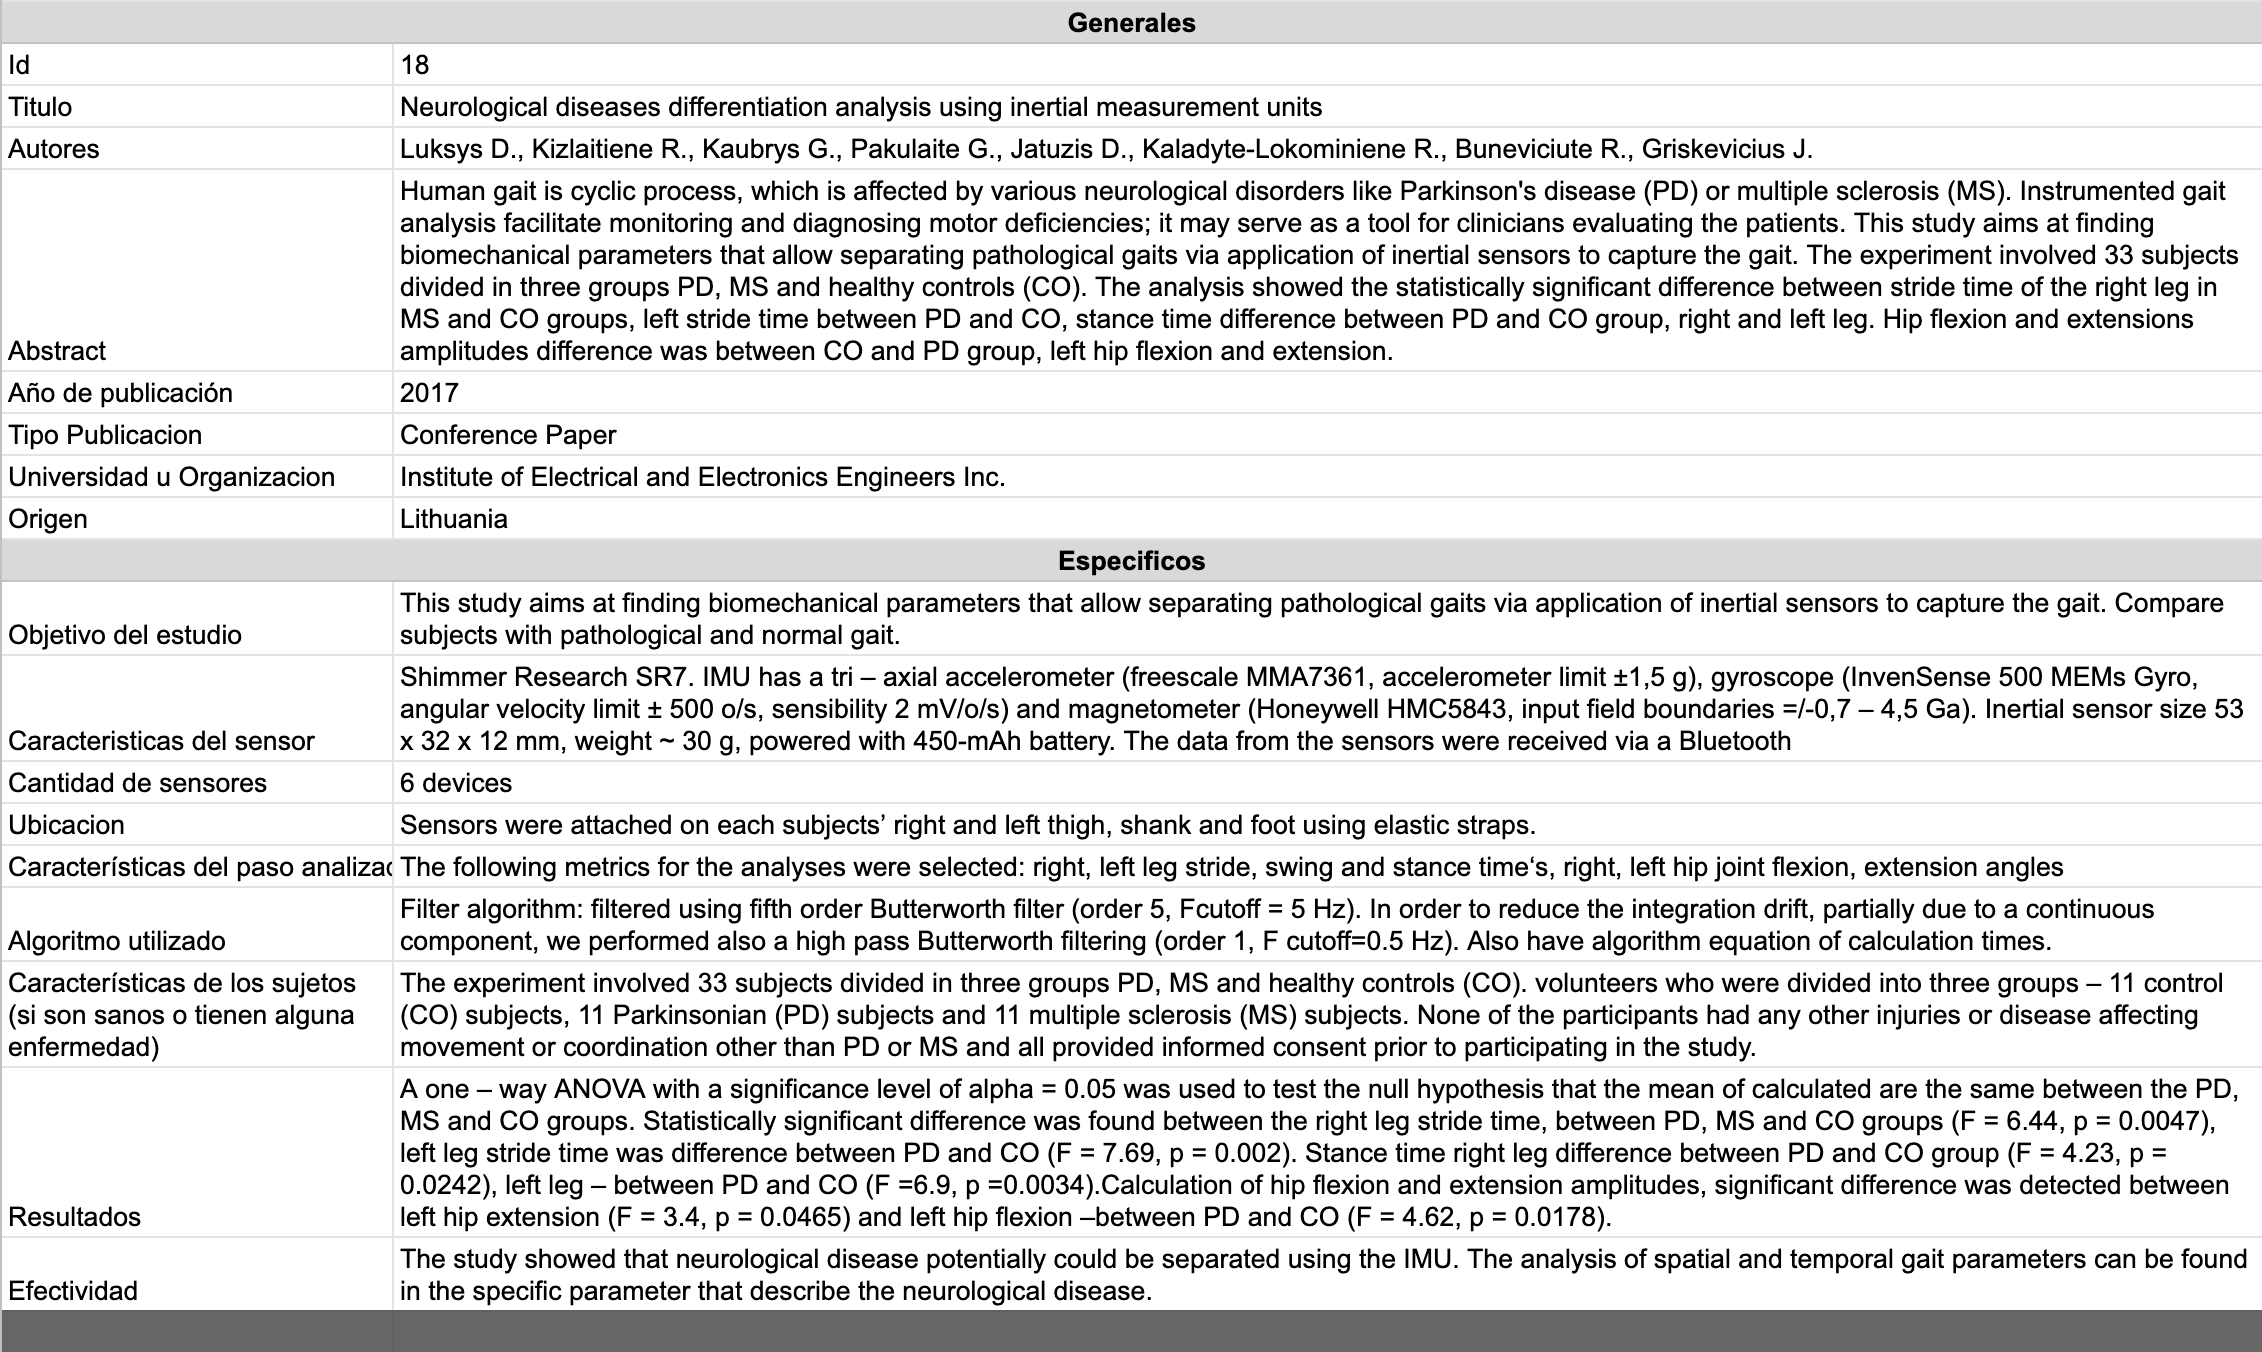
\includegraphics[scale=0.48]{TESIS/imagenes/chap03/extraction-3.png}
\end{minipage}}
\end{center}
\caption{Formulario de extracción empleado en PARKIBIP. }
\label{fig:extraction}
\end{figure} 

\section{Síntesis: Resultados primarios}\label{synthesis}

Teniendo en cuenta el tiempo planificado para la etapa de análisis de la literatura, se priorizó sintetizar el conjunto de investigaciones pertenecientes a la Categoría 1 (30) cuyo aporte tendrá gran relevancia para el proyecto PARKIBIP, tal como indica la tabla Tab.\ref{tab:selection_results}. Con el objetivo de responder las preguntas planificadas se analizó: el año de publicación, el objetivo, las características de los sensores utilizados, la cantidad y ubicación de los sensores, las características del paso analizadas y los algoritmos computacionales empleados para dicho fin, las características de los sujetos -sanos o con alguna patología-.

Más allá del estado del arte respecto al uso de dispositivos IMU para analizar la marcha de las personas al caminar -objetivo central-, resulta útil para los productores y consumidores de la investigación conocer las diversas salidas para la investigación y el crecimiento del campo de estudio. Así, en primera instancia se realizó una clasificación previa de los artículos en base a cuatro criterios:
\begin{enumerate}
    \item Fecha de Publicación
    \item Países involucrados en las investigaciones
    \item Tipo de Publicación
    \item Editorial
\end{enumerate}

%  Fecha de Publicación
La búsqueda realizada se focalizó en los años 2016 al 2019. Esta decisión se debió a que los avances tecnológicos han avanzado considerablemente en los últimos años, por lo tanto, no es relevante para este estudio el análisis de artículos con más de 4 años de antigüedad.
La figura Fig. \ref{fig:synthesis_year} presenta la distribución de estudios primarios por año de publicación. La razón de que exista un único estudio publicado para el año 2019 es trivial -mismo año que la presente LSR-; sin embargo, se observa un buen numero de estudios para los restantes años.

\begin{figure}[H]
\centering
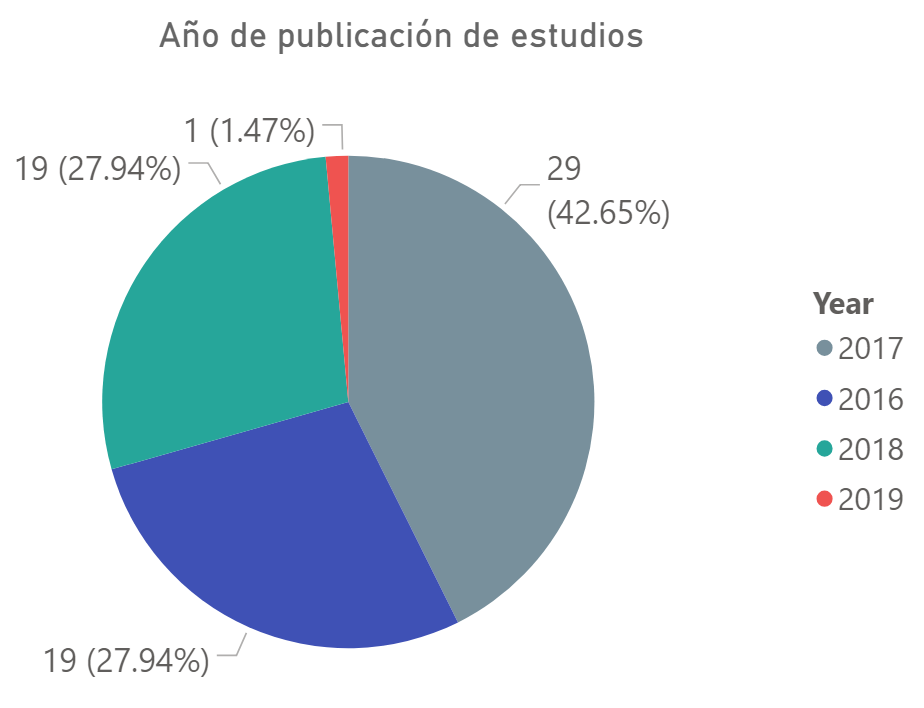
\includegraphics{TESIS/imagenes/chap03/sintesis_anio.PNG}
\caption{Distribución de estudios primarios por año.}
\label{fig:synthesis_year}
\end{figure}

% Países
Resulta importante identificar los países interesados en la materia, ya sea para compartir el conocimiento adquirido y trabajar colaborativamente, o simplemente Benchmarking. En la figura Fig. \ref{fig:synthesis_countries} se presenta la distribución de países involucrados en las investigaciones. Existe una gran prevalencia de investigaciones con origen Italiano (7) indicando un fuerte campo de interés para dicho País. Asimismo, se puede apreciar una buena dispersión de estudios primarios (31) por Países (18) -aprox. 60\% de países distintos-, lo que infiere la importancia compartida del campo de estudio entre países y pocas investigaciones realizadas.    

\begin{figure}[H]
\centering
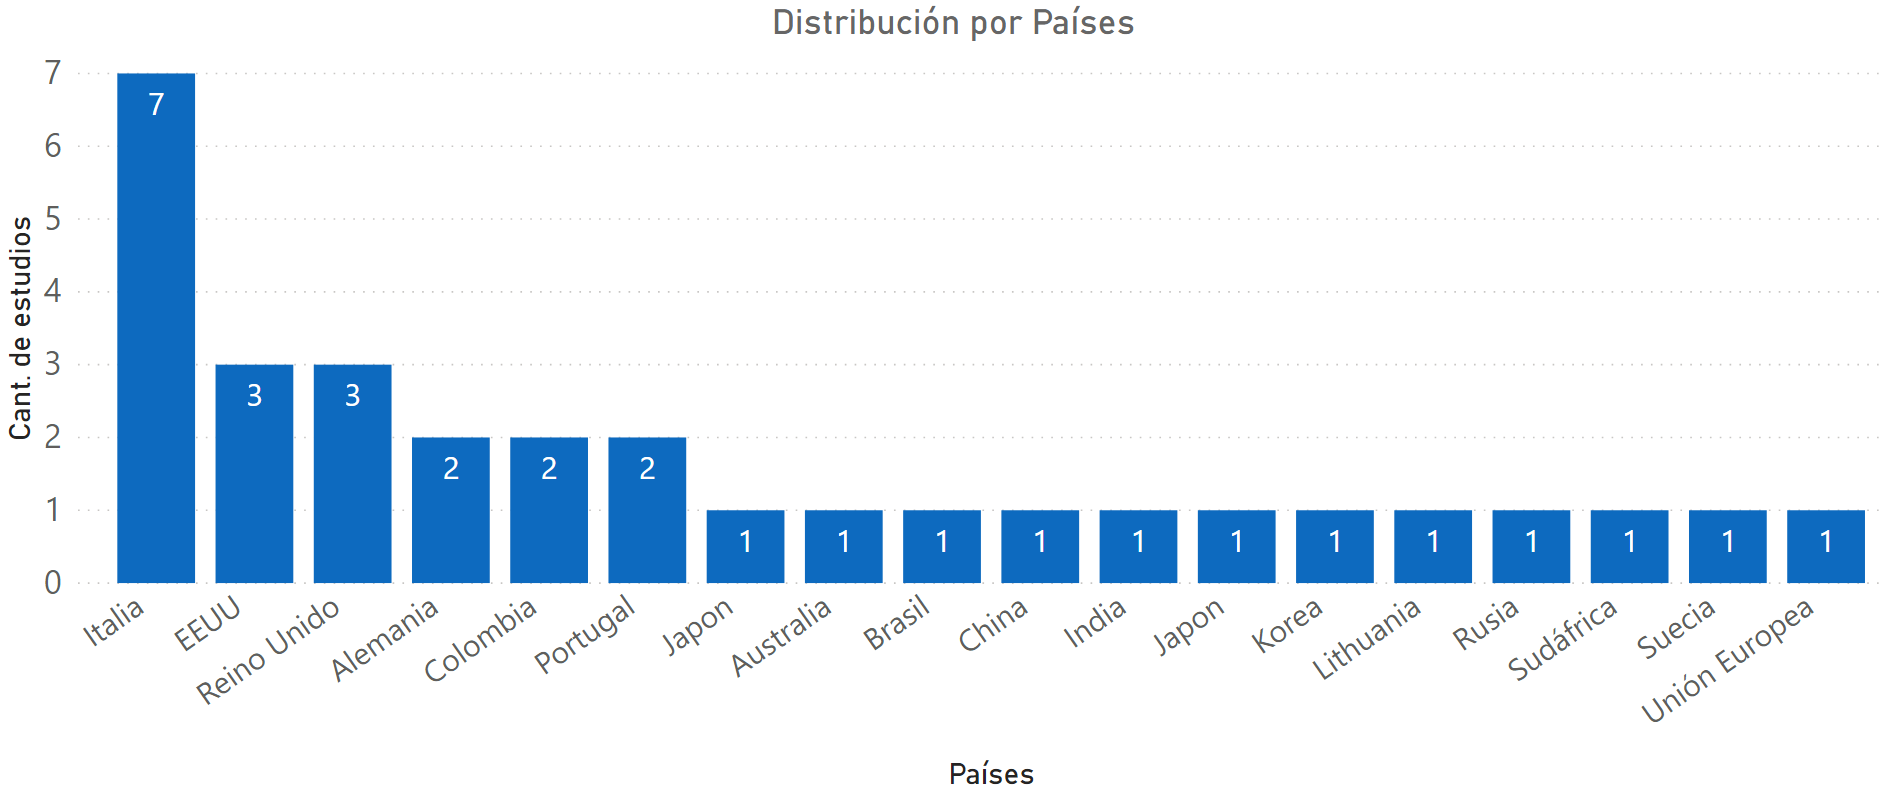
\includegraphics[width=\textwidth]{TESIS/imagenes/chap03/sintesis_country.PNG}
\caption{Gráfico de los países de origen de las investigaciones.}
\label{fig:synthesis_countries}
\end{figure}

% Tipo de Publicación 
Por su parte los artículos analizados fueron publicados tanto en conferencias como en revistas de manera proporcional, con el análisis de una revisión sistemática respecto a las distintas particiones existentes del ciclo de la marcha, y la inclusión del capitulo de un libro. Además, dichas publicaciones fueron fragmentadas por casa editora, siendo la asociación profesional de ingeniería electrónica e ingeniería eléctrica (IEEE) la de mayor presencia con el 50\% de publicaciones aproximadamente. Las figuras Fig. \ref{fig:synthesis_publicationType}\ref{fig:synthesis_publicationEditorial}.

\begin{figure}[H]
\centering
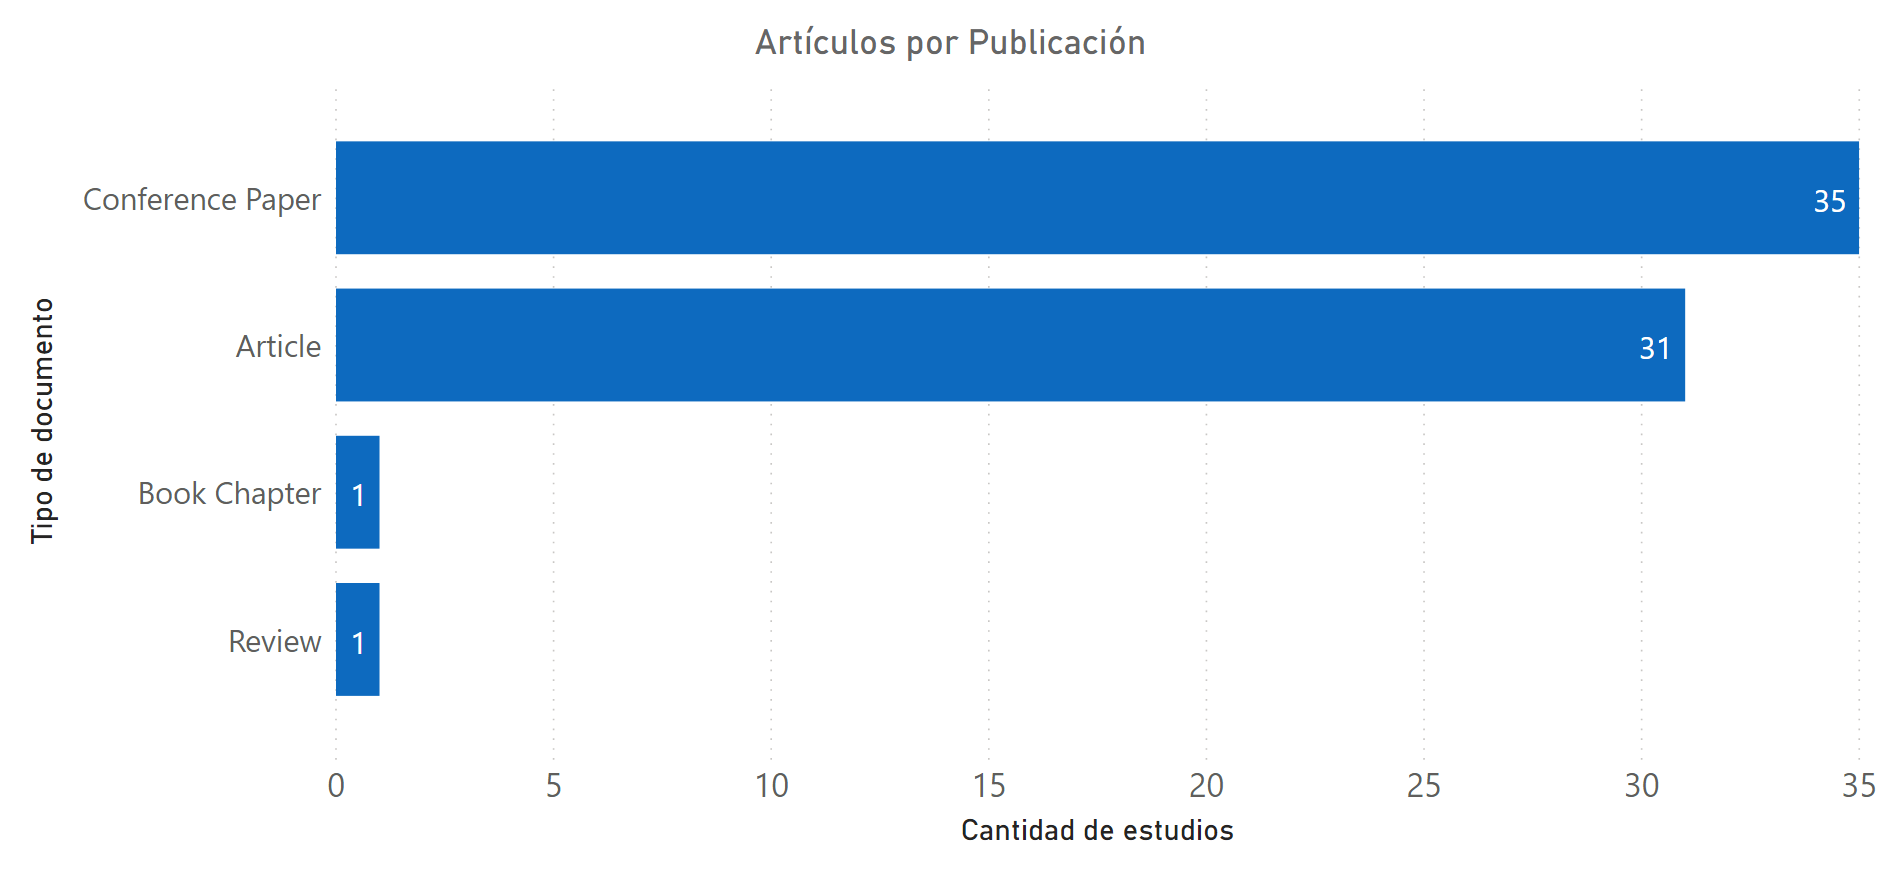
\includegraphics[width=\textwidth]{TESIS/imagenes/chap03/sintesis_documentType.PNG}
 \caption{Artículos sobre análisis de la marcha por tipo de publicación.}
 \label{fig:synthesis_publicationType}
\end{figure}

%Editorial
\begin{figure}[H]
 \centering
 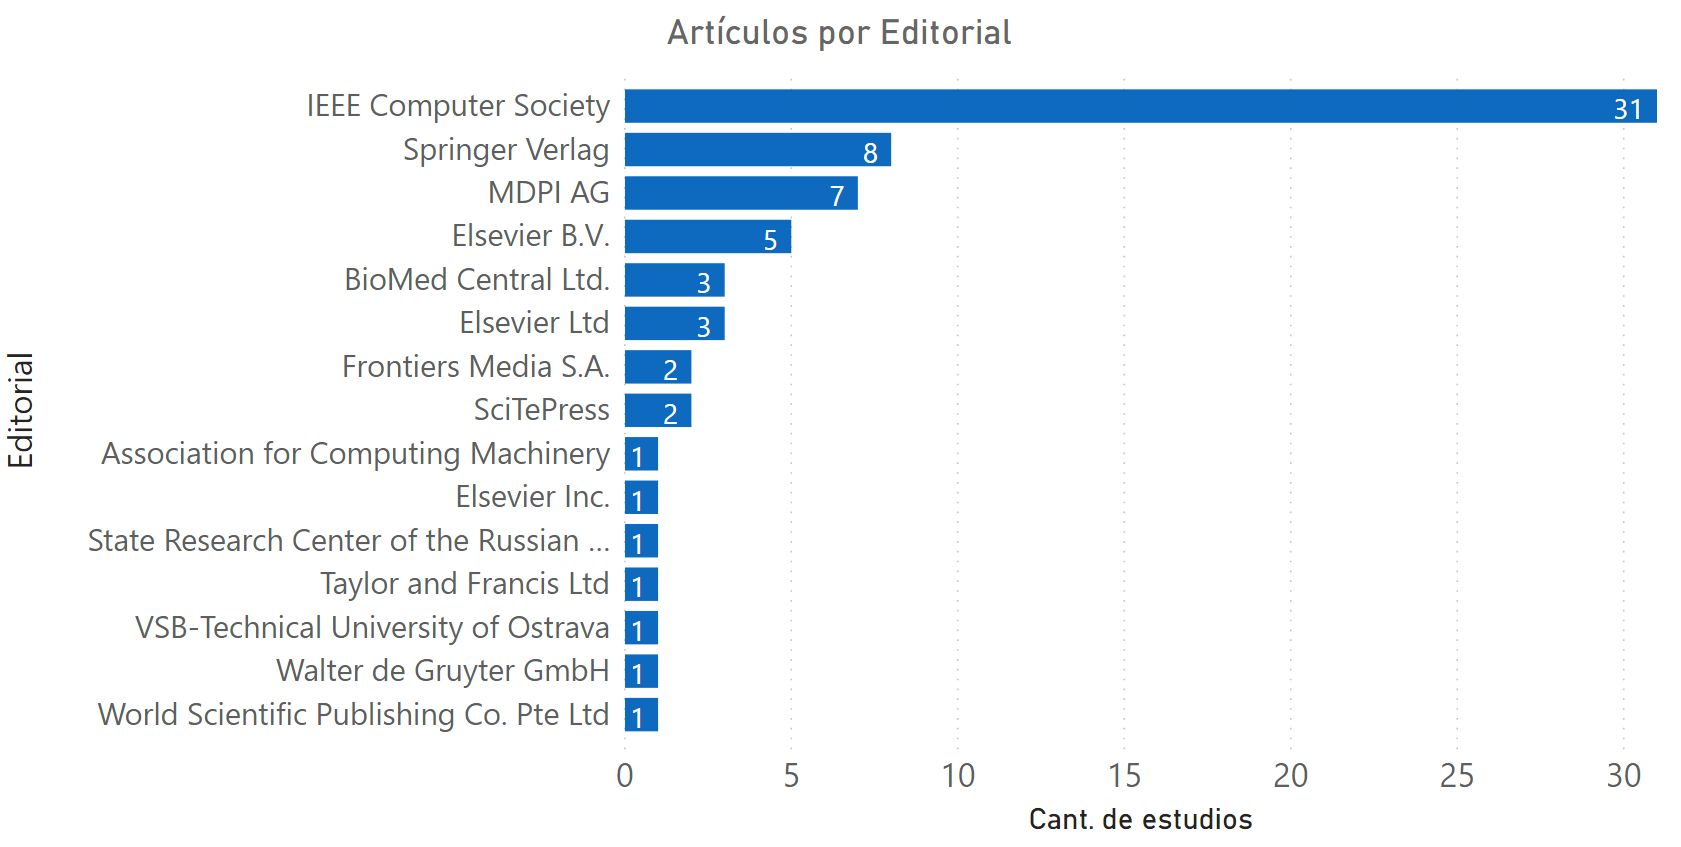
\includegraphics[width=\textwidth]{TESIS/imagenes/chap03/sintesis_editorial.PNG}
 \caption{Artículos sobre análisis de la marcha por editorial.}
 \label{fig:synthesis_publicationEditorial}
\end{figure}

Desde la perspectiva de la revisión sistemática realizada, es importar abordar las preguntas de investigación elaboradas en el objetivo con la finalidad de adquirir conocimiento, contemplar dificultades y riesgos, producir ventajas de la evidencia recolectada.

% 1.Caracteristicas de IMUs
Ya mencionado, los dispositivos IMU pueden contar con diversos sensores de medición; en su forma mas básica cuentan con un acelerómetro. En general, salvo en las investigaciones cuya información no fue especificada, la mayoría de los estudios usaron dispositivos IMU con 9/6 DOF (sus siglas del ingles, refieren a los grados de libertad, variables independientes) de diversas compañías; integrando la combinación de un acelerómetro y giroscopio tridimensionales, en algunos casos también un magnetómetro tridimensional. Es relevante notar que, todos los dispositivos empleados tienen como salida datos en la unidad correspondiente al sensor y sin procesar; de ahí la necesidad de algoritmos específicos al caso de uso.

% 2.Cuántos sensores son necesarios para medir la marcha? 
Según el área de estudio particular dentro de la marcha de las personas, las investigaciones emplearon entre 1 y 7 dispositivos IMU. Aproximadamente el 86.5\% de los estudios requirió dos o mas dispositivos, en donde prevalece con el 50\% el uso de dos dispositivos. La figura Fig. \ref{fig:synthesis_devices} sintetiza el numero de dispositivos que fueron necesarios para realizar cada investigación.

\begin{table}[H] 
\caption{Cantidad de dispositivos empleados para analizar la marcha de personas según los artículos contemplados.}
\centering
\begin{tabular}{| p{4cm} | p{4cm} |}
\hline
\textbf{Dispositivos IMU (en unidades)} & \textbf{Artículos (en unidades)}\\ \hline
1 & 4\\ \hline
2 & 12\\ \hline
3 & 6 \\ \hline
4 & 2 \\ \hline
5 & 1 \\ \hline
6 & 3 \\ \hline
7 & 1 \\ \hline
\textbf{Total} & \textbf{28}\\ \hline
\end{tabular}
 \label{fig:synthesis_devices}
\end{table}

\noindent A priori, se podría concluir que empleando un único dispositivo inercial sería suficiente para analizar la marcha de las personas y elevar los costos y las complejidades con otros adicionales. Sin embargo, éste resultado subjetivo no es correcto; y como fue mencionado, la cantidad de dispositivos necesarios depende de las variables de estudio dentro del ``gait analysis'' -i.e. según partición del ciclo de la marcha, parámetro espacio-temporal particular (aceleración, velocidad, etc.), simetría entre pasos, rotación tobillo, entre otras-. Sumado a la anterior afirmación, se debe contemplar los algoritmos computacionales empleados, la ubicación del dispositivo, la cantidad de variables de la marcha a analizar para dicha ubicación, la efectividad reportada para esa variable de estudio. Por ejemplo, un único dispositivo ubicado en el centro de masa -a la altura de la pelvis- podría detectar si existe movimiento, en cambio, no se podría estudiar el ciclo de la marcha en 2 fases Stance (fase de apoyo) y Swing (fase de vuelo) por pie y por lo tanto limitando los parámetros espacio-temporales de los mismos.

% 3.Que ubicaciones utilizan los dispositivos?
Similar a lo mencionado, la ubicación anatómica del dispositivo en el cuerpo humano tiene gran relevancia y determina/limita el espectro de estudio. La figura Fig. \ref{fig:synthesis_location} con sus respectivas sub-figuras, resume las distintas ubicaciones anatómicas empleadas para posicionar al menos un IMU, así como también sus distintas configuraciones que permiten el ``gait analysis''. Las mismas, exhiben que si bien las posiciones anatómicas son variadas y aproximadamente el 33\% localiza al menos un IMU en la Tibia; según las configuraciones, en su mayoría se localiza únicamente en el pie del sujeto en cuestión.

\begin{figure}
     \centering
     \begin{subfigure}[b]{1\textwidth}
         \centering
         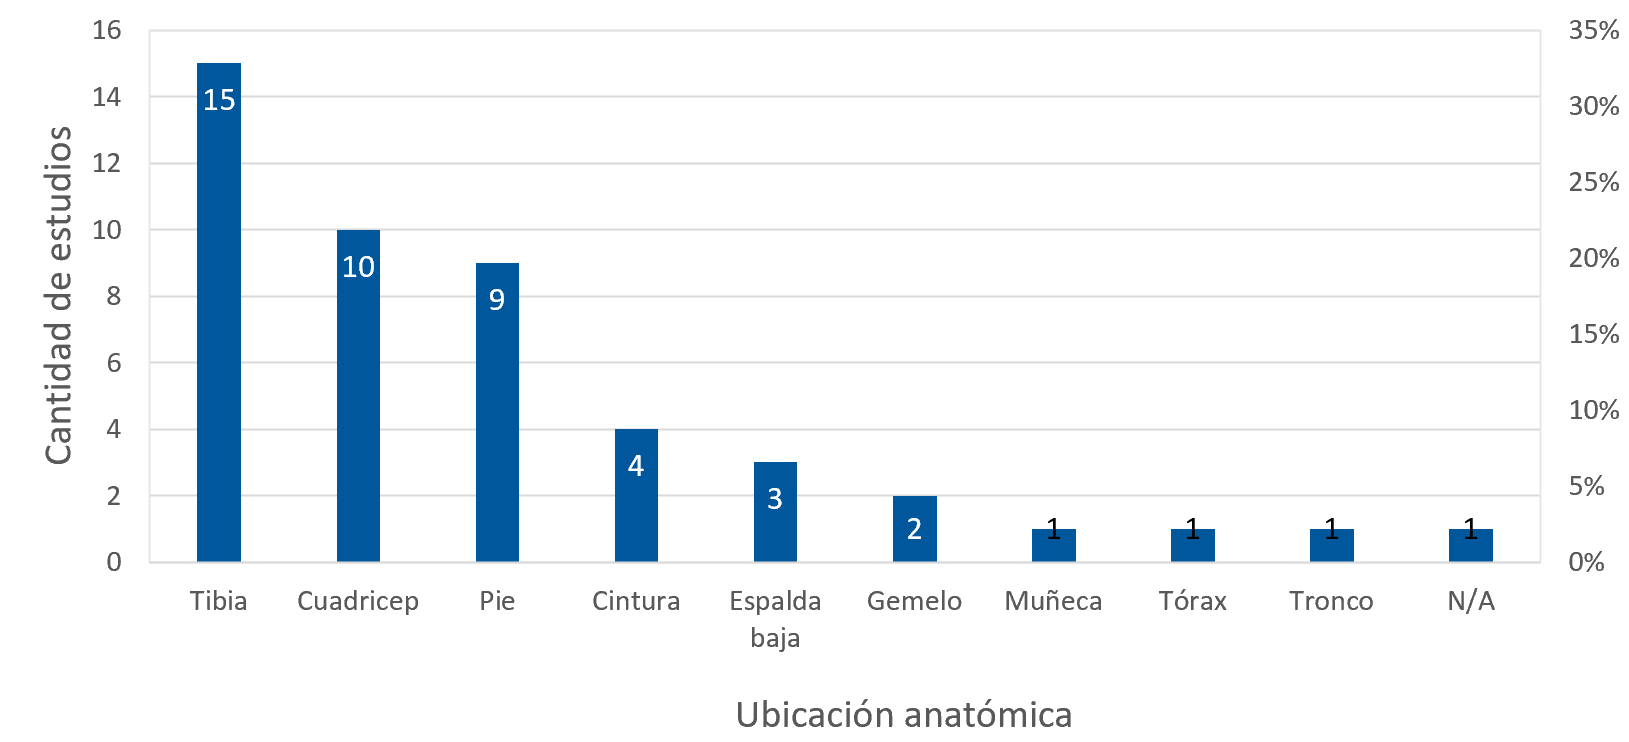
\includegraphics[width=\textwidth]{TESIS/imagenes/chap03/ubicaciones-anatomicas.PNG}
         \caption{Ubicaciones anatómicas empleadas para posicionar al menos un IMU en el análisis de la marcha de personas. Según la evidencia, aproximadamente el 33\% de estudios emplea la Tibia, luego el Cuádricep y el Pie del sujeto con un $\approx$20\%. }
     \end{subfigure}
     \begin{subfigure}[b]{1\textwidth}
        \centering
        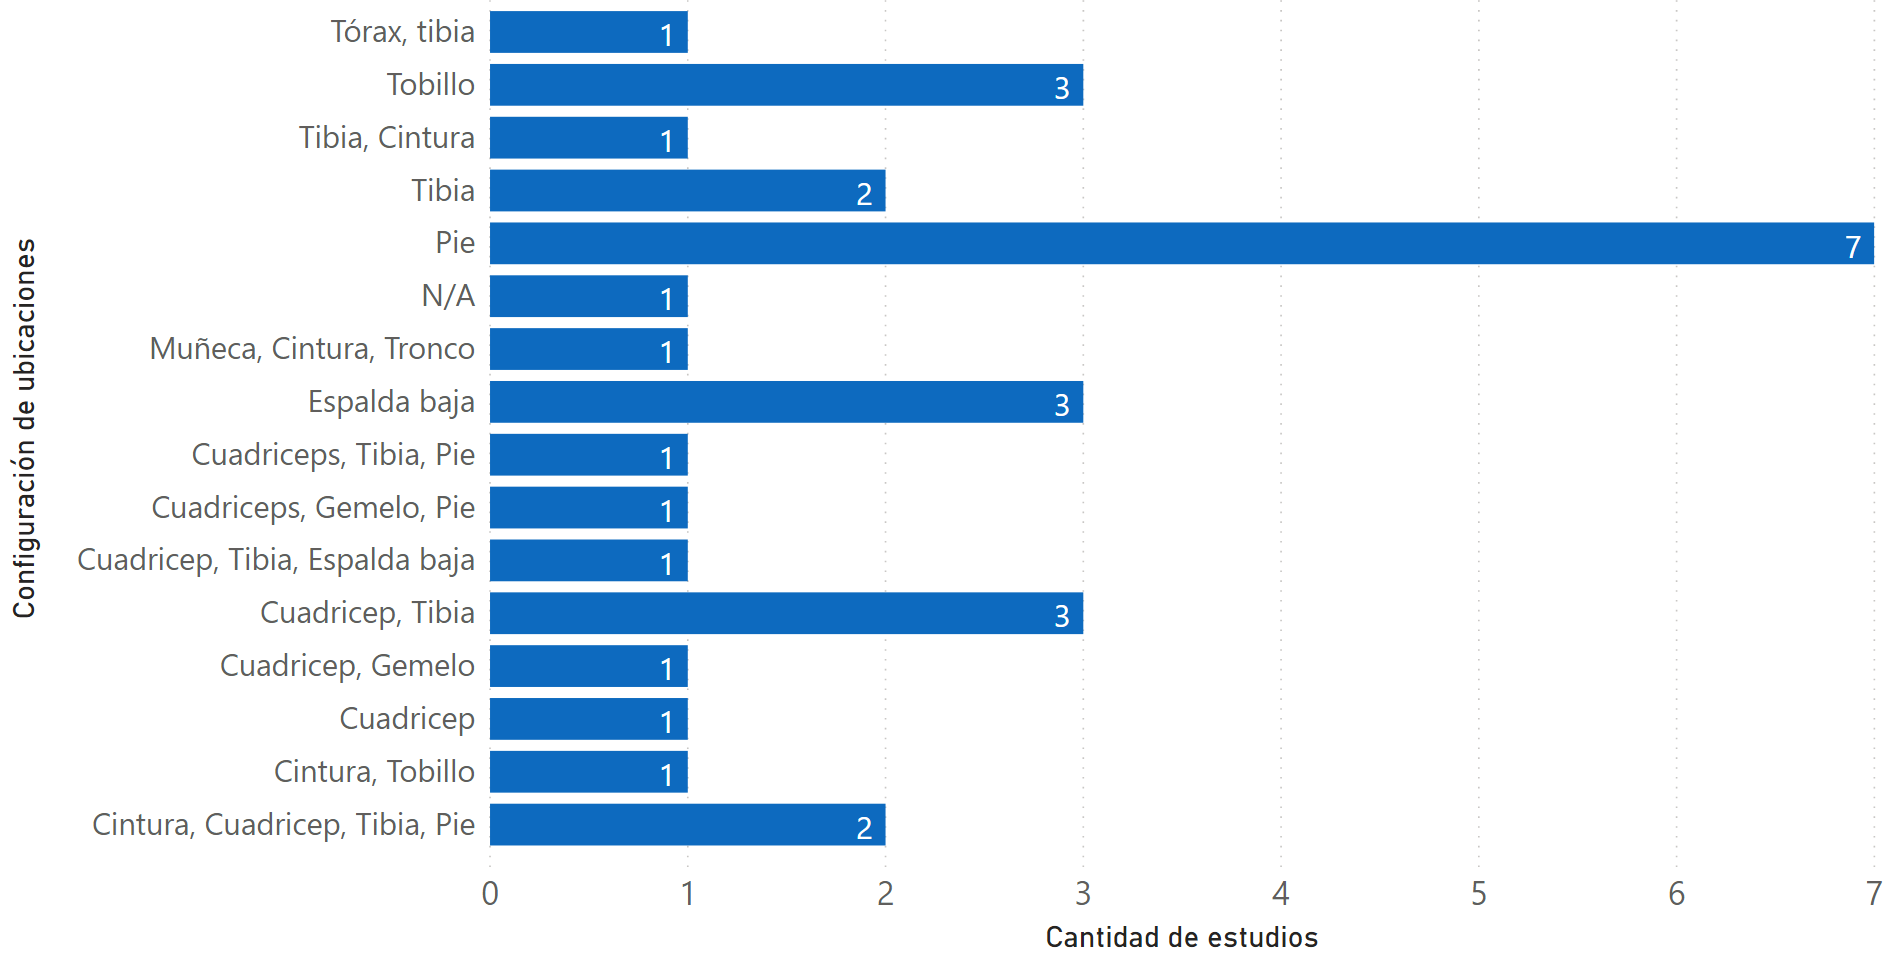
\includegraphics[width=\textwidth]{TESIS/imagenes/chap03/sintesis_location.PNG}
        \caption{Configuraciones de ubicaciones anatómicas para posicionar los IMU que permiten analizar la marcha de un sujeto.}
     \end{subfigure}
     \caption{Ubicaciones de dispositivos IMU en el cuerpo de los sujetos para el análisis de la marcha, según los distintos estudios de la revisión sistemática.}
     \label{fig:synthesis_location}
 \end{figure}


Combinando los resultados anteriores -cantidad y ubicación en el cuerpo- sobre los dispositivos empleados, se puede afirmar que la mayoría de estudios empleó dos dispositivos IMU localizados en el pie del sujeto particular. Además, dicha ubicación permite abordar los problemas esenciales:
\begin{itemize}
    \item Identificar el ciclo de la marcha por extremidad
    \item Estudiar diversos parámetros espacio-temporales por extremidad o de forma general
\end{itemize} 

% 4.Qué datos sobre la marcha se pueden obtener con los distintos sensores?

Por otro lado, resulta crucial para la investigación entender \textbf{de qué forma se procesan los datos}, \textbf{qué eventos se detectan} para distinguir las distintas etapas de la marcha y \textbf{qué tipo de parámetros se pueden obtener} con cada tipo de análisis. La tabla Tab. \ref{tab_synthesis_algorithm} enumera 
los datos mencionados para cada uno de los 30 artículos analizados.

{\fontsize{9}{11}\selectfont
\setlength\LTleft{-2.5cm}
\begin{longtable}{|p{1cm}|p{4cm}|p{2.5cm}|p{3.5cm}|p{6cm}|}
\hline
\label{tab_synthesis_algorithm}
\textbf{ID} & \textbf{Nombre del artículo} & \textbf{Eventos detectados} & \textbf{Algoritmo utilizado} & \textbf{Parámetros obtenidos} \\ \hline
\endhead
1 & Gait evaluation using inertial measurement units in subjects with Parkinson's disease & Heel Strike, Toe Off & Double Integration. High pass filter. Butterworth filter. & Cadence (steps/min). Mean velocity (m/s). Stride length (m). Stride duration (s). Step duration (\%). Stance phase duration (\%). Swing phase duration (\%). Double support phase duration (\%). \\ \hline
2 & Towards a portable human gait analysis \& monitoring system & Heel Strike, Toe Off & Double Differential and Integration, ZUPT & Steps. Kinematic angles in Sagittal, Transverse and Frontal planes. \\\hline
3 & Trainer in a pocket - Proof-of-concept of mobile, real-time, foot kinematics feedback for gait pattern normalization in individuals after stroke, incomplete spinal cord injury and elderly patients & Heel Strike, Toe Off & Kalman Filter - ZUPT & Stride length. Foot to ground angle. Stance time. Swing time \\ \hline
4 & Validity of shoe-type inertial measurement units for Parkinson's disease patients during treadmill walking & Heel Strike, Toe Off
 & Double Integration. Butterworth filter. & Cadence. Step length. Step time \\ \hline
5 & Estimation of spatio-temporal parameters of gait from magneto-inertial measurement units: Multicenter validation among Parkinson, mildly cognitively impaired and healthy older adults & Heel Strike, Toe Off & Custom method* & Stride duration. Step duration. Cadence \\ \hline
6 & Optimal Foot Location for Placing Wearable IMU Sensors and Automatic Feature Extraction for Gait Analysis & Heel Strike, Toe Strike, Heel Off, Toe Off & Trapezoidal Double Integration. Butterworth filter. & Times of stance, swing, single and double support; stride length and stance phase; gait velocity, stride duration, cadence and step length; step number, moving distances, instant step speed and average speed; step counting; times of heel strike, toe strike, heel-off, and toe-off; stride length and duration; walking distance, time and speed \\ \hline
7 & The clinical application of inertial measurement unit in identification of foot drop symptoms & Heel Strike, Toe Off & Custom method* & Cadence, step length, foot to ground angle \\ \hline
8 & An Automatic gait feature extraction method for identifying gait asymmetry using wearable sensors & Heel Strike, Toe Strike, Heel Off, Toe Off & Trapezoidal Double Integration. Butterworth filter. & Stride length and stance phase; gait velocity, stride duration, cadence and step length; step number, moving distances, instant step speed and average speed; step counting; times of heel strike, toe strike, heel-off, and toe-off; stride length and duration; walking distance, time and speed \\ \hline
9 & IMU-based gait analysis for rehabilitation assessment of patients with gait disorders & Heel Strike, Flat foot, Midstance, Heel off, Toe Off, Midswing, Heel Strike & Peak detection, ZUPT & Cadence, Symmetry \\ \hline
10 & Real-time tool for human gait detection from lower trunk acceleration & Heel Strike, Flat foot, Toe Off, Midstance, HO & Double Integration, State Machine, Exponential Filter. & Cadence, step time \\ \hline
11 & The application of inertial measurements unit for the clinical evaluation and assessment of gait events & Heel Strike, Toe Off & Sensor Fussion, State Machine.
Butterworth low pass filter & Steps. Dorsiflexion angle \\ \hline
12 & Validation of a new model-free signal processing method for gait feature extraction using inertial measurement units to diagnose and quantify the severity of Parkinson's disease & Heel Strike, Toe Off & Low pass and high pass filters
Madgwick filter to calculate the orientation.
Double Integration & Cadence, stride length, stride velocity, range of motion, joint angles, maximum swing velocity, sit to stand and stand to sit transition times, turn time, turn peak velocity, etc. \\ \hline
13 & Validation of a step detection algorithm during straight walking and turning in Patients with Parkinson's disease and older adults using an inertial measurement unit at the lower back & Heel Strike, Toe Off & CWT - Continuous wavelet transform & Steps \\ \hline
14 & L-DOPA and freezing of gait in Parkinson's disease: Objective assessment through a wearable wireless system & Heel Strike, Toe Off.FOG (Freezing of gait) & Proportional Integral Controller Filter.
Custom method for orientations and events detection & Step velocity (centimeters per second) was defined as the distance covered by the leg in time unit; stride length (centimeters), the distance between two consecutive heel strike of the same foot; stride time (seconds), the time from initial contact of one foot to subsequent contact of the same foot; and finally, cadence (steps per minute) was defined as the number of steps per minute. \\ \hline
15 & Assessing the accuracy of an algorithm for the estimation of spatial gait parameters using inertial measurement units: Application to healthy subject and hemiparetic stroke survivor & Heel Strike, Toe Off & Madgwick orientation
Double Integration - ZUPT & cadence, walking speed, stride length, step length, and timing of the different stages of the gait cycle. More \\ \hline
16 & The development and concurrent validity of a real-time algorithm for temporal gait analysis using inertial measurement units & Heel Strike, Toe Off & Noise-Zero Crossing algorithm NZC & GCT = Gait Cycle Time, SLS = Single Limb Support Time, DLS = Double Limb Support Time. \\ \hline
17 & Neurological diseases differentiation analysis using inertial measurement units & Heel Strike, Toe Off, Midstance. 
Max. Flexion, min. extension. & Butterworth low and high pass filter.Double Integration & Right, left leg stride, swing and stance time‘s, right, left hip joint flexion, extension angles. \\ \hline
18 & A wearable wireless system for gait analysis for early diagnosis of Alzheimer and Parkinson disease & Heel Strike, Toe Off & Low pass and high pass filter. Complementary Filter. Double pendulum model. & Stride number Mean stride length
Standard deviation stride Standard deviation stance Mean swing Standard deviation swing Cadence Step time \\ \hline
19 & Linear progression measurement and analysis of human gait for the development of a multifunctional robotic walker & Heel Strike, Toe Off & Low pass and high pass filters. Double Integration. & Steps, distance, velocity, time \\ \hline
20 & Knee joint angle monitoring system based on inertial measurement units for human gait analysis & Knee joint angle & No specified & N/A. Just compare with other methods results. \\ \hline
21 & Efficient techniques for gait-analysis: Comparing marker-less and imu-based tracking systems for monitoring rehabilitation processes & The oscillations of the medio-lateral center of mass (CoM). & Kalman Filter + ZUPT & Velocity, step or stride length and cadence. \\ \hline
22 & A practical step length algorithm using lower limb angular velocities & Heel Strike, Toe Off, MSt and MSw & Inverted Pendulum Model algorithm & Step time, Gait velocity, Stride length \\ \hline
23 & An IMU-to-Body Alignment Method Applied to Human Gait Analysis & Heel Strike, Toe Off & Joint Angles Calculation with Joint Coordinate System (JCS) & Knee flexion angle, ankle angle, hip flexion angle \\ \hline
24 & Proposal of a short step and stride measurement system for uncontrolled environments & Loading response, Midstance, Terminal Stance, Preswing, Initial Swing, Midswing, Terminal Swing & Quaternion orientation with gravity removal.
Trapezoidal Double Integration & Short step length, Stride length \\ \hline
25 & Gait event detection in laboratory and real life settings: Accuracy of ankle and waist sensor based methods & Heel Strike, Toe Off & Custom method & stride time, step time and stance time \\ \hline
26 & Technical challenges using magneto-inertial sensors for gait analysis & Not specified & Not specified & Not specified \\ \hline
27 & Inertial BSN-Based Characterization and Automatic UPDRS Evaluation of the Gait Task of Parkinsonians & Heel Strike, Toe Off & Butterworth low pass filter. & Gait Cycle Time, Stance Time, Swing Time.
Stride length, stride velocity, step length, step velocity. \\ \hline
28 & Estimation of foot trajectory during human walking by a wearable inertial measurement unit mounted to the foot & Heel Strike, Midstance, Toe Off & Gravity removal. Double Integration & Step-by-step stride length \\ \hline
29 & Motion Monitoring based on a Finite State Machine for Precise Indoor Localization & Heel Strike, Midstance, Toe Off & Orientation with euler angles. ZUPT - Kalman Filter. & Distance, stride length \\ \hline
30 & Handling gait impairments of persons with Parkinson’s disease by means of real-time biofeedback in a daily life environment & Not specified & Not specified & Distance, cadence, stride length, stride duration, gait speed \\ \hline
\end{longtable}
\normalsize}
% 5.Qué técnicas o algoritmos se utilizan para analizar los datos?

% 5.1 - Eventos detectados 


Respecto a los eventos detectados, la amplia mayoría de los artículos (89.2 \%) detecta los eventos de Heel Strike y Toe Off. Estos eventos son suficientes para dividir el ciclo de marcha en sus fases principales: Stance (apoyo) y Swing (vuelo). Un  60.7 \% de los artículos detecta únicamente estos dos eventos. Algunos estudios necesitan estudiar la marcha con mayor granularidad, otros necesitan analizar otros aspectos; a continuación se listan los diferentes eventos estudiados en todos los artículos: 

\begin{itemize}
    \item Heel Strike: Apoyo del talón 
    \item Heel Off: Despegue del talón 
    \item Toe Strike: Apoyo de los dedos 
    \item Toe Off: Despegue de los dedos 
    \item Midstance: Mayor apoyo del pie 
    \item Knee max. flexion: Máxima flexión de la rodilla 
    \item Knee min. extension: Extensión mínima de la rodilla
    \item FOG - Freezeing of gait: Bloqueo de la marcha 
    \item Pre swing: Etapa inicial en fase de vuelo del pie 
    \item Mid swing: Etapa intermedia en fase de vuelo 
    \item Terminal swing: Etapa final en fase de vuelo
    \item La oscilación del centro de masa medio-lateral
\end{itemize}

% Los que no dan info útil

Como se puede observar en la tabla Tab. \ref{tab_synthesis_algorithm}, se han utilizado una gran variedad de algoritmos para el estudio de la marcha. Algunos de estos estudios [20, 26, 30] no especificaron la forma con la que obtienen los resultados. Otros [5, 7, 25] utilizaron métodos personalizados, basados en heurísticas y máquinas de estados.

% Cálculo de la orientación - Mahony, Madgwick, etc.

Una primera etapa en el análisis de la marcha consiste en el cálculo de la orientación de cada dispositivo IMU. La orientación del dispositivo debe conocerse con un alto grado de precisión para que las mediciones de gravedad se puedan distinguir de la aceleración física del sensor. Incluso pequeños errores en la estimación de la orientación producirán errores extremadamente altos en la aceleración medida, lo que se traduce en errores aún mayores en las estimaciones de velocidad y posición. Para los artículos estudiados, algunos de los métodos utilizados son: la construcción de matrices de rotación en base a los ángulos de Euler, el método sugerido por Martin \& Salaun \cite{Martin2010}, la técnica propuesta por Mahony \cite{Mahony2006} y el filtro propuesto por S. Madgwick \cite{Madgwick}. 

% Detección de eventos - Double Integration

Para el análisis de la marcha mediante la detección de eventos, uno de los métodos más utilizados es el de \textbf{Doble Integración (DI)}. Este método fue utilizado por el 44.4 \% de los artículos que reportan el algoritmo utilizado [1, 4, 6, 8, 10, 12, 15, 17, 18, 19, 24, 28]. Es el método más simple entre los reportados, tanto con su implementación a través del método del Trapecio, como con el método de Simpson. Consiste en Integrar la aceleración para obtener la velocidad, para luego realizar una nueva integración y obtener el desplazamiento. Este método por si solo no es para nada suficiente, ya que, por un lado es necesario conocer las condiciones iniciales, y por otro, existe un error de integración que es incremental y acumulativo. Este error debe ser removido con algún otro método. Con este propósito se utilizan distintos tipos de filtros como: High Pass Filter, Low Pass Filter, Butterworth filter, etc. 

% Detección de eventos - ZUPT

Uno de los métodos utilizados para reducir el error acumulado es el \textbf{Zero Velocity Update} (ZUPT, por sus siglas en inglés). Se basa principalmente en la detección de los intervalos de tiempo en los cuales el sistema está en una fase estacionaria, es decir, cuando el sistema tiene una posición y una orientación constante. El uso de actualizaciones de velocidad cero es especialmente atractivo para limitar el error en los sistemas donde los dispositivos que se encuentran montados a los pies del sujeto, ya que durante el ciclo de la marcha el pie vuelve a un estado estacionario.

% Detección de eventos - Kalman filter

Algunos de los estudios aplicaron ZUPTs a \textbf{Kalman Filter} para mejorar la solución de navegación. El filtro de Kalman no solo estima el error de velocidad en los intervalos ZUPT detectados, sino que también estima las correcciones de posición, altitud y sesgo de los sensores inerciales debido a correlaciones cruzadas en la matriz de transición.

% Detección de eventos - Resto

El resto de los métodos relevados para detectar los eventos de la marcha son variados. Algunos están basados en máquinas de estado, otros en detección de picos, otros utilizan el cálculo de ángulos articulares utilizando un sistema de coordenadas articulares, por mencionar algunas de estas variantes (ver en tabla Tab. \ref{tab_synthesis_algorithm}).

Resulta interesante conocer los distintos parámetros espacio temporales que se obtienen en cada estudio mediante los algoritmos antes mencionados. Estos parámetros son el resultado final del análisis de la marcha. Los estudios tienen como objetivo analizar estos parámetros que caracterizan la marcha de los sujetos y seleccionan los algoritmos adecuados para obtener estos parámetros. 

A continuación, se nombran los principales parámetros que se obtuvieron como resultado utilizando los distintos algoritmos:
\newline\newline
\noindent\fbox{
     \parbox{\textwidth}{
    \textit{
    Cadencia (pasos/min), Velocidad media (m/s), Velocidad instantánea (m/s), Longitud de zancada (m), Longitud de paso (m), Duración del paso (s), Duración de la zancada (s), Duración de fase de apoyo simple (\%), Duración de fase de vuelo (\%), Duración de fase de apoyo doble (\%), Cantidad de pasos; Ángulos cinemáticos en planos Sagital, Transverso y Frontal; Distancia recorrida (m), Tiempo total (s), Ángulo de dorsiflexión; y más. 
    }
    }
}
\newline\newline
% 6.Subjects
En cuanto a las características de los sujetos convocados para efectivizar las pruebas experimentales para cada investigación, en promedio se realizaron pruebas sobre unos 36 sujetos. Como se puede visualizar en la gráfica de la Fig. \ref{fig:subjects-age}, la gran mayoría de los estudios optan por realizar las pruebas con sujetos de todas las edades, tanto jóvenes como adultos mayores; sin embargo, solamente cuatro estudios hicieron pruebas únicamente con jóvenes y otros cuatro estudios únicamente con adultos mayores. 

\newpage

\begin{figure}[H]
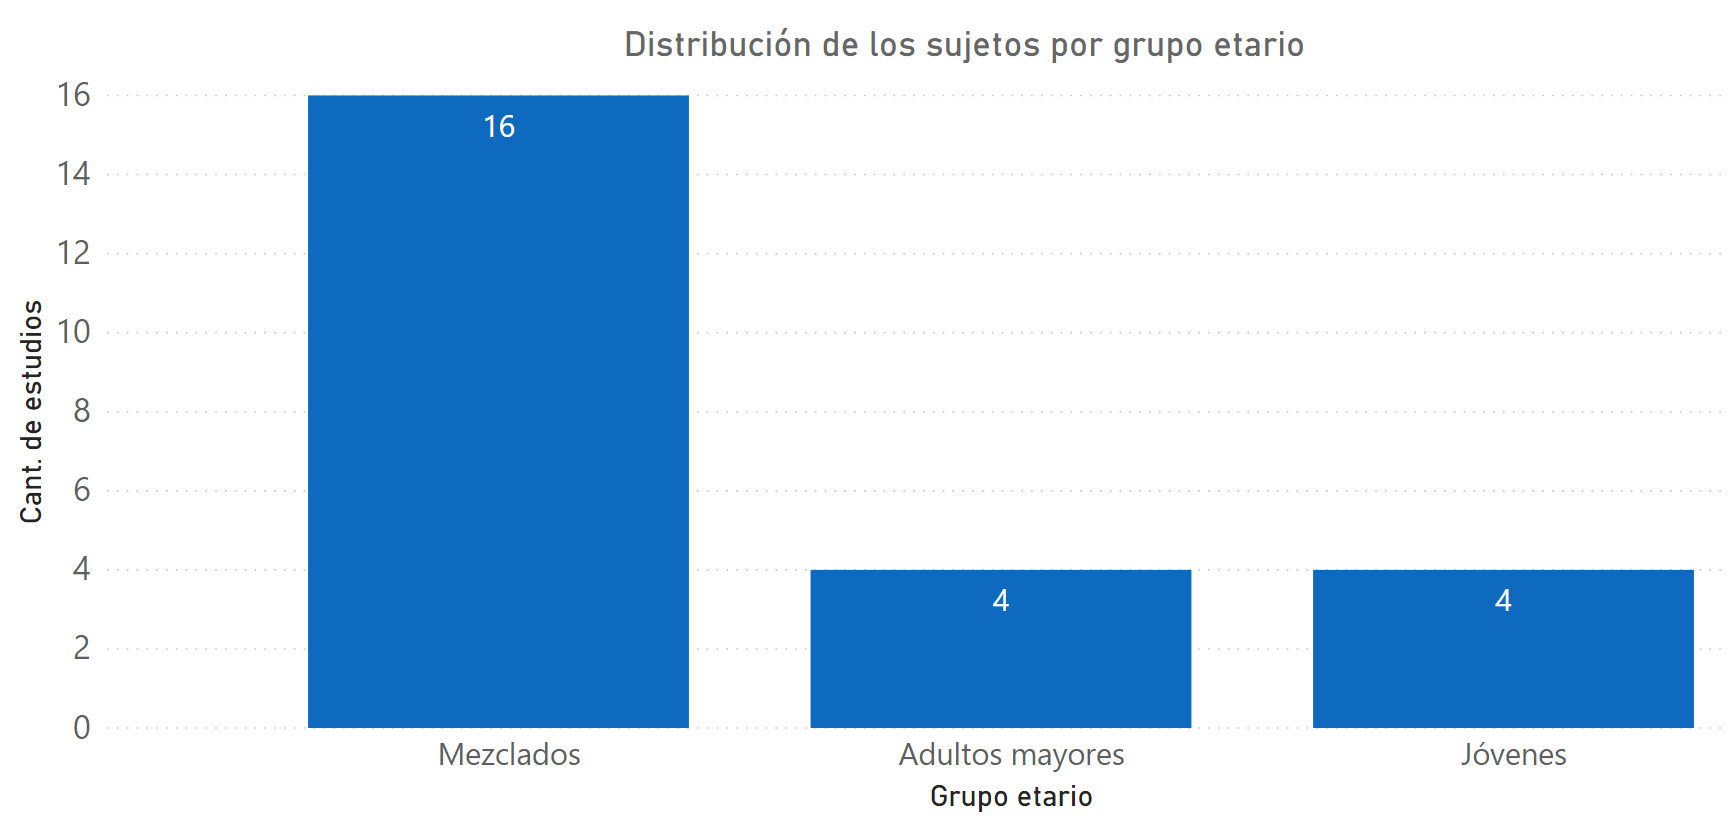
\includegraphics[width=\textwidth]{TESIS/imagenes/chap03/sintesis_grupoEtario.PNG}
\caption{Resumen de la población de estudio por grupo etario.}\label{fig:subjects-age}
\end{figure}

Respecto a la condición de clínica de los sujetos participantes, se puede observar una ligera inclinación a realizar pruebas con personas completamente sanas (41.7\%), aunque existe una proporción muy parecida de los estudios que se realizaron con sujetos enfermos (25\%) o con ambas condiciones (33.3\%) -ver gráfica en Fig. \ref{fig:subjects-condition}-. 

\begin{figure}[H]
\centering
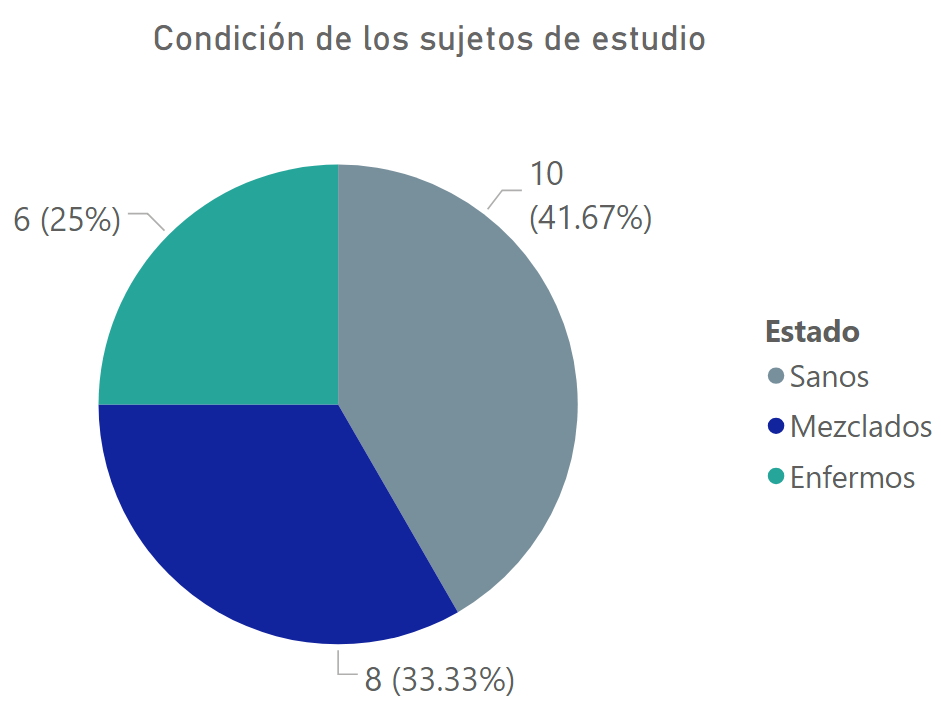
\includegraphics{TESIS/imagenes/chap03/sintesis_subjects.PNG}
\caption{Resumen de condición sobre la totalidad de sujetos en cada estudio}
\label{fig:subjects-condition}
\end{figure}

\noindent Las métricas obtenidas respecto a los sujetos de las pruebas en las distintas investigaciones responden al contexto de investigación, en su totalidad son estudios de ``gait analysis'' con una finalidad médica, aunque no todos para una alteración de la marcha. Por lo tanto, no necesariamente se requieren pruebas con sujetos enfermos.

\section{Limitaciones}\label{synthesis_2}

El presente estudio integra distintos conceptos que requieren un nivel medio a alto de entendimiento, como los son los algoritmos físico-matemáticos necesarios para detectar los eventos del ciclo de la marcha -HS, TO, Stance, Swing-, los métodos numéricos capaces de estimar los parámetros espacio-temporales (i.e. velocidad de la marcha), la biomecánica, y el manejo de múltiples señales de los distintos sensores del IMU. Se reconoce el no cumplimiento de estos requerimientos y un aprendizaje en el transcurso de la SLR. 

En muchos casos no fue posible acceder al estudio completo. Este tipo de situaciones se da cuando la temática tratada tiene un alto impacto comercial y es necesario abonar una suma de dinero a cambio del material completo.

En general, los artículos analizados se enfocan en innovación, presentan una nueva combinación de técnicas para predecir eficazmente alguna de las fases del ciclo de la marcha o al menos un parámetro espacio-temporal. Si bien algunos investigadores proponen nuevos modelos, los esfuerzos se centran principalmente en encontrar y optimizar técnicas de estimación.

\section{Resultados secundarios}

Consecuentemente, se obtuvieron diversos resultados sumamente valiosos, que no fueron planificados al inicio del proyecto mediante preguntas de investigación. De esta manera, se listan los resultados adicionales de la revisión sistemática realizada:
\begin{enumerate}
    \item \underline{Identificación de las compañías de soluciones de sensores.} De gran utilidad para efectuar una amplia comparación de dispositivos existentes en el mercado y poder seleccionar el adecuado.
    \item \underline{Posiciones oportunas del IMU en el pie.} Las estimaciones resultantes de los algoritmos numéricos se ven afectadas por la localización del dispositivo en el cuerpo a sensar. De esta manera, se pudo analizar las distintas localizaciones que lograron mejores resultados y contemplarlas en la solución. 
    \item \underline{Particionamiento del ciclo de la marcha.} Se constato la diversidad de granularidades de las fases de la marcha (i.e. dos,tres, cuatro, cinco, seis, siete y ocho) cada una con sus ventajas y desventajas; la cual permite definir las fases necesarias y suficientes a identificar mediante el sistema PARKIBIP.
    \item \underline{Métodos de estimación de fases de la marcha.} Existen diversos algoritmos innovadores para estimar las fases del ciclo de la marcha, que serán tenidos en cuenta para lograr una solución eficaz.
    \item \underline{Métodos de estimación de parámetros espacio-temporales.} Similar al punto previo, se detectaron variadas técnicas innovadores para estimar los parámetros espacio-temporales de la marcha. En ambas ocasiones, no existe una regla de oro, y todo indica que el campo de estudio es emergente.
    \item \underline{Requerimiento de un algoritmo eficaz de orientación.} Trabajar con el movimiento de un cuerpo particular mediante dispositivos sujetos al mismo, requiere la identificación de la orientación de los dispositivos -por ende la del cuerpo-, respecto a un sistema de referencia inercial (en general, el sistema tierra). Existen diferentes métodos para computar la orientación, basados en rotaciones clásicas hasta sistemas complejos como el gradiente descendente. Es sabido que, en los sistemas de gait analysis, un cuello de botella para estudiar parámetros de la marcha es logra un resultado sumamente eficaz de la orientación del cuerpo respecto al sistema de referencia inercial. Será uno de los desafío de PARKIBIP obtener tal resultado.
    \item \underline{Conocimiento, desafíos y riesgos.} El hecho de analizar detalladamente diversas investigaciones (aproximadamente 85) trae como consecuencia directa la adquisición de conocimiento, por consiguiente las dificultades y riesgos a contemplar y mitigar durante el transcurso del proyecto. Como por ejemplo la implementación de un filtro eficaz y eficiente de Orientación, frecuencias adecuadas por tipo de sensor (acelerómetro, giroscopio, magnetómetro), la necesidad de algoritmos de predicción para parámetros espacio-temporales (es decir, si bien se cumplen las leyes mecánicas, las mismas no son aplicables computacionalmente por el error cuadrático acumulativo). 
\end{enumerate} % Se carga el capítulo Revisión sistemática
  \chapter{Proyecto: Decisiones de diseño}\label{chap:project} %Materiales y métodos

La finalidad del presente capitulo es explicitar el proceso de investigación y toma de decisiones llevado a cabo durante el proyecto PARKIBIP, mediante los cuales se obtienen los resultados, y por tanto el cumplimiento -parcial o total- de los objetivos establecidos. A partir de las cualidades desafiantes del proyecto, las incertidumbres respecto al contexto clínico y de análisis -marcha de sujetos con EP-, y los objetivos preestablecidos; se optó por conducir durante todo el proyecto una investigación científica, rigurosa, orientada al entendimiento del contexto y a minimizar riesgos -SLR realizada-. De esta manera, todo aquel material, procedimiento o método arbitrario fue descartado mediante un proceso de evaluación de calidad.

\section{Selección tecnológica}\label{seleccion_tecnologica}

En primera instancia y como disparador, se elaboró una revisión de la evidencia científica existente vinculada a los avances tecnológicos y a su aplicación en la detección de las fases de la marcha en personas, con el fin de definir el tipo de dispositivo adecuado a emplear en PARKIBIP (i.e. plantillas inteligentes, unidad de medición inercial, etc.). La misma, se ejecutó en el portal en línea Timbó, el cual habilita a acceder a la última bibliografía y literatura científica-tecnológica mundial reportada.

Para seleccionar la tecnología a utilizar, se consideró una revisión sistemática realizada en el año 2016 \cite{Taborri2016}, la cual identifica, selecciona y categoriza las distintas tecnologías para realizar la detección de las fases del paso, analizando ventajas y desventajas de cada solución. De esta manera, la selección del tipo de sensor se realizó teniendo en cuenta características relevantes para el proyecto en cuestión, entre ellas, el costo, la accesibilidad, la efectividad y la portabilidad del dispositivo.

Bajo los criterios mencionados, el tipo de dispositivo elegido que mejor se adecúa al proyecto fue un dispositivo IMU (del inglés Inertial Measurement Unit o Unidad de Medición Inercial). Estos dispositivos portables, de bajo costo y larga autonomía, han sido utilizados con buenos resultados en el área de análisis de movimientos dinámicos lineales y angulares en los últimos años. Se componen esencialmente de los sensores acelerómetro, giroscopio y magnetómetro, y en ciertos casos se extienden a incluir barómetro, sensores de luz, entre otros.

\section{Estudio de factibilidad} %Metodología de investigación 
Luego de seleccionar el tipo de dispositivo a utilizar, se tomo la decisión de realizar una \textbf{revisión sistemática de la literatura (SLR) respecto al uso de sensores IMU para analizar la marcha de las personas al caminar}. El objetivo de una revisión sistemática es buscar e identificar todo el material relevante relacionado con un tema determinado conforme a responder las preguntas de investigación, siguiendo una metodología objetiva, analítica y tan repetible como sea posible. De acuerdo con los procedimientos descritos en el capítulo de fundamentos, apartado \nameref{fundamentos:RSBE}.

Los principales factores de motivación que impulsaron a aplicar esta metodología fueron:

\begin{itemize}
    \item Adquirir conocimiento respecto a la problemática. Por ejemplo el contexto clínico, el análisis de la marcha y sus fases, la aplicación de sensores IMU y sus desafíos, algoritmos numéricos reportados -matemáticos y computacionales-, entre otros
    \item Corroborar la propiedad innovadora del proyecto -no exista otra que aborde el mismo tema-
    \item Estudiar la marcha de las personas 
    \item Reducir o eliminar incertidumbres en la investigación
    \item Identificar recomendaciones a seguir para PARKIBIP
    \item Identificar las principales metodologías y técnicas aplicadas
\end{itemize}

Si bien elaborar una SLR es un proyecto en sí  mismo, el cual requiere mucho esfuerzo y dedicación, realizarla fue sumamente valiosa y se justifica plenamente tanto con los factores de motivación expuestos como con la obtención de sus resultados en la sección \nameref{synthesis} de la SLR.

El capitulo \nameref{chap_RSBE}, describe el procedimiento completo de la SLR aplicada a la realidad de PARKIBIP, y una variación de sus etapas -de acuerdo al proyecto-. Además, presenta los resultados primarios que responden las preguntas de investigación planificadas, como también los resultados secundarios -no preestablecidos- derivados del análisis pormenorizado del conocimiento relevado.

Bajo el soporte fundamentado de la SLR elaborada, se toman las decisiones pertinentes con el fin de mitigar los riesgos y lograr construir PARKIBIP. Los resultados alcanzados actúan como guía de conclusiones a tomar, algunos puntos son: (i) Proveedores de HW, (ii) Cantidad de dispositivos IMU y ubicación en el cuerpo, (iii) Granularidad de fases a detectar como eventos, (iv) Posibles algoritmos numéricos, (v) Filtro de Orientación eficaz y eficiente.

\section{Benchmark: Elección del dispositivo IMU}\label{section:imu-selection}

Durante el transcurso del estudio de factibilidad y adquisición de conocimiento llevado a cabo mediante la revisión sistemática, se analizaron los distintos proveedores de hardware especializados en soluciones de sensores embebidos. Recordando que, no se encuentra dentro de los objetivos la construcción de una dispositivo de HW -por ende no pertenece al alcance del Proyecto-, fue necesario seleccionar la tecnología (Sec.\ref{seleccion_tecnologica}) a emplear y posteriormente elegir el proveedor de hardware que mejor se adecua a Parkibip.

Existen en el mercado decenas de empresas que ofrecen estos dispositivos junto a sus distintas variaciones, por lo que surgió la necesidad de hacer una evaluación de mercado y elegir la más apropiada. La Tabla comparativa Tab.\ref{tab:imus}  permite visualizar las principales características evaluadas.

\begin{table}[!h]
\caption{Comparación de dispositivos IMU}
\label{tab:imus}
\centering
\hspace*{-3.5cm}%
\begin{tabular}{p{2cm}|p{0.8cm}|p{0.8cm}|p{1cm}|p{1cm}|p{1cm}|p{1cm}|p{1cm}|p{1.2cm}|p{1cm}|p{1cm}|p{1cm}|p{0.8cm}}
 & Arion & BTS G-Sensor & EXL S3 & Inven- Sense & Isen & MMR & Opal APDM Inc & Reha- Gait (HASOMED) & Senno- Gait SmartInsolesPRO & Shim- mer Sensor & Wave- share & Xsens   \\ \hline
Acelerómetro (3-axis) & SI & SI & SI & SI & SI & SI & SI & SI & SI & SI & SI & SI \\ \hline
Giroscopio (3-axis) & SI & SI & SI & SI & SI & SI & SI & SI & SI & SI & SI & SI \\\hline
Magnetómetro (3-axis) & NO & SI & SI & SI & SI & SI & SI & SI & SI & SI & SI & SI \\ \hline
Barómetro & SI & NO & NO & NO & SI & SI & NO & - & NO & NO & SI & NO \\ \hline
Altímetro & - & - & - & NO & NO & SI & - & - & NO & SI & NO & NO \\ \hline
Bluetooth & SI & SI (3.0) & SI (2.1) & NO (I2C, SPI) & NO & SI (LE) & NO & SI & SI & SI & NO & - \\ \hline
Wifi & NO & NO & NO & NO & SI & NO & NO & NO & SI & NO & NO & NO \\ \hline
Tiempo Real & SI & SI & SI & SI & SI & SI & \textless 30ms & - & - & - &  & \textless 2 ms \\ \hline
Runtime calibration & NO & NO & NO & SI & SI & SI & - & - & - & SI &  & - \\ \hline
Peso & - & 37gr & 22g & - & 46g & 8.5 g & \textless 25g & - & - & 23.6g & 3g & - \\ \hline
Medidas (mm) & - & 70 x40 x18 & 54 x33 x14 & 3 x3 x0.9 & 56 x38 x18 & 24 x17 x4 & 43 x39 x13 & 60 ×15 ×35 & 35-45 & 51 x34 x14 & 31 x16 x2.5 & 57 \\ \hline
Batería & $\sim$7hs & $\sim$8hs & 2 hs & - & $\sim$3.5 hs & 2-14d & 8-16hrs & - & \textgreater{}48hrs & - & - & - \\ \hline
SDK Android & NO & NO & NO & SI & SI & SI & No & NO & NO & SI &  & SI \\ \hline
SDK iOS & NO & NO & NO & NO & NO & SI & No & NO & NO & NO &  & NO \\ \hline
Comunidad OpenSource & NO & NO & NO & SI & NO & SI & NO & NO & NO & NO &  & NO \\\hline
Documenta-ción & NO & NO & NO & SI & NO & SI & NO & NO & NO & SI &  & SI \\ \hline
Vibración & NO & NO & NO & NO & NO & SI & NO & NO & NO & NO &  & NO \\ \hline
Precio & \euro 189 & - & - & - & - & USD99 & - & - & - & \euro 359 & USD16 & \euro 800 \\ \hline
\end{tabular}
\hspace*{-3.5cm}%
\end{table}

%Dispositivos, sensores usados
A efecto de la etapa, se concluyó en la utilización de la solución de producto de dispositivos vestibles MetaMotionR (MMR). Además de ser un dispositivo liviano, accesible y de bajo costo; integra los principales sensores de lectura, como lo son el acelerómetro (BMI160 6-Ejes), el giroscopio (BMI160 6-Ejes), el magnetómetro y la unidad vibratoria. 

\section{Cantidad y ubicación del dispositivo}

Se cree pertinente emplear dos dispositivos IMU sincronizados, unidos con bandas elásticas de velcro a los tobillos -justo por encima de los maléolos- de los pacientes con la enfermedad de Parkinson tal como indica la Fig. \ref{FIG:foot_strap}. De esta manera, es posible estudiar el comportamiento y las distintas variables vinculadas a cada extremidad por separado, así como combinarlas para lograr otros resultados genéricos. De forma complementaria, la decisión logra un espectro o visión de análisis mas amplio, el cual habilita a escalar el alcance del proyecto en materia de variables de la marcha o patologías (i.e. rotaciones, asimetrías, etc.).

\begin{figure}[h!]
\centering
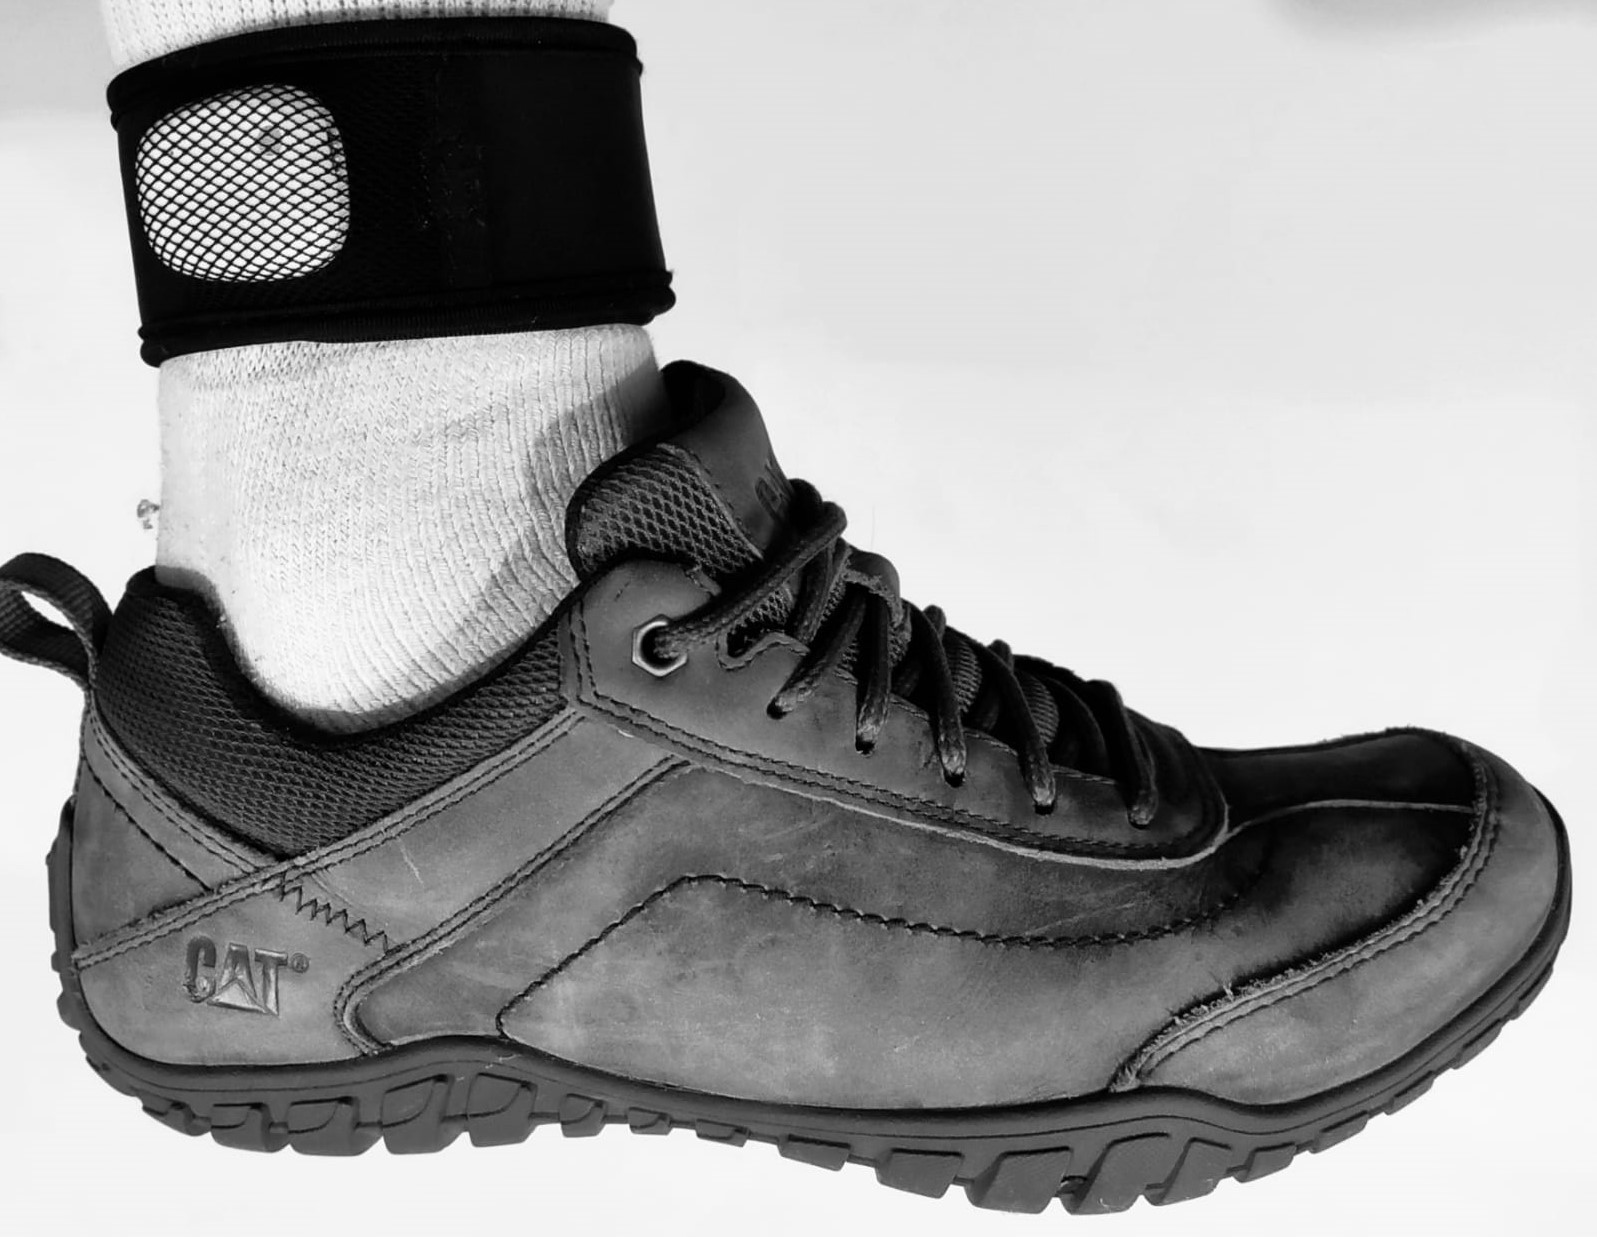
\includegraphics[clip,width=0.78\columnwidth]{TESIS/imagenes/img/footstrap.jpeg}
\caption{Banda elástica junto a la unidad de medición inercial (IMU).}
\label{FIG:foot_strap}
\end{figure}

\section{Granularidad de fases de la marcha} \label{section:partition-cycle}

%Fases de la marcha y las que vamos a identificar.
Estandarizando los conceptos de fases de la marcha, tal como se sintetiza en \cite{Taborri2016}, se pueden emplear distintas granularidades de las fases de la marcha (i.e. dos, tres, cuatro, cinco, seis, siete y ocho), tal como indica la Fig. \ref{FIG: ciclo}.

\begin{figure}[h!]
\centering
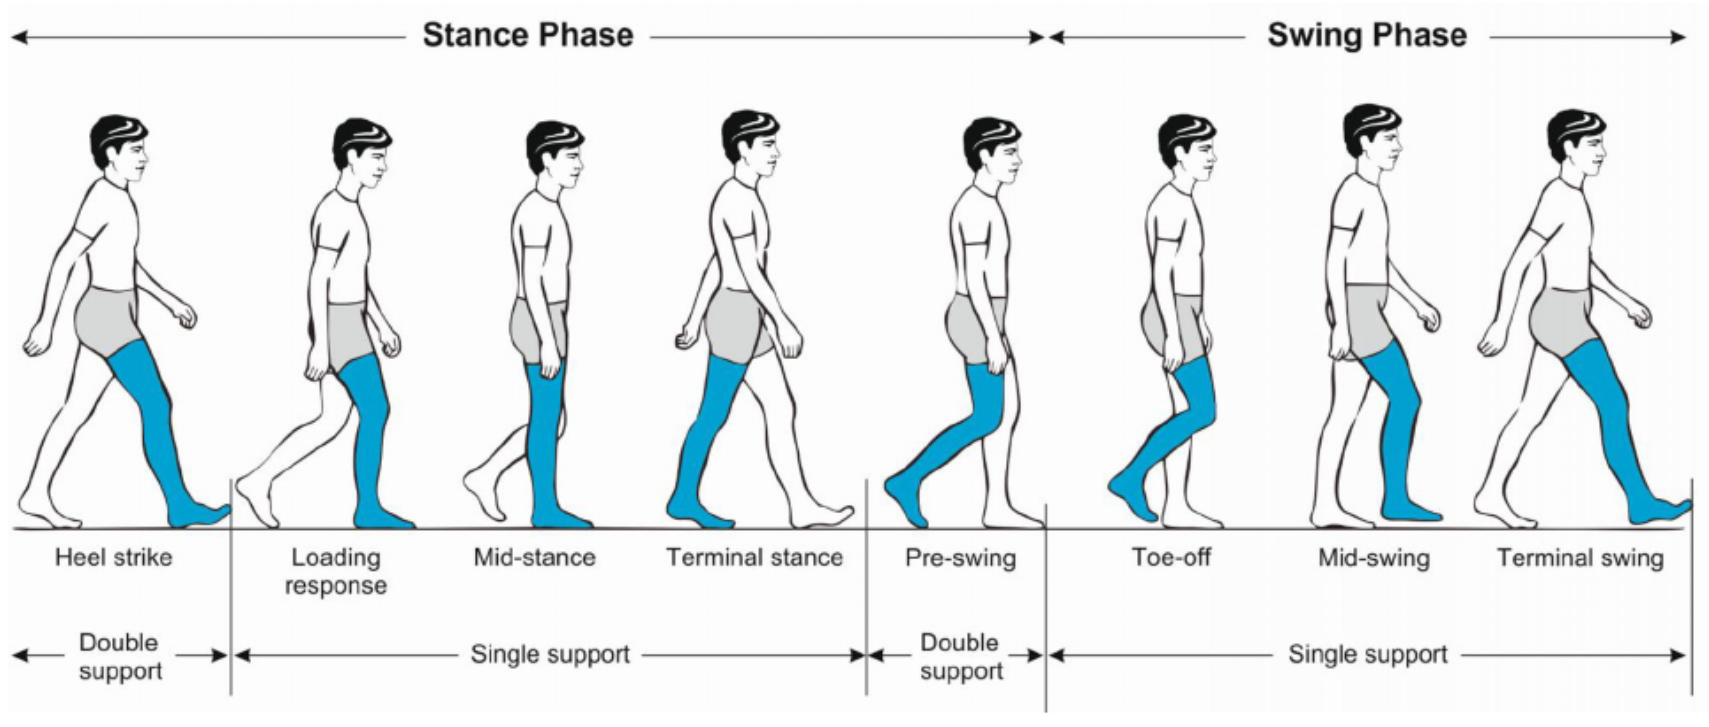
\includegraphics[clip,width=1.05 \columnwidth]{TESIS/imagenes/img/gaitcycle.png}
\caption{Partición del ciclo de la marcha normal en 8 fases. Tomado de ``W. Pirker y R. Katzenschlager'' \cite{Pirker2016}.}
\label{FIG: ciclo}
\end{figure}

El presente proyecto reconoce dos fases en el ciclo de la marcha, fase de apoyo y fase vuelo. En este sentido, los algoritmos matemáticos considerados se enfocan en detectar eficazmente los eventos golpe de talón (HS, del ingles Heel Strike) y el despegue de los dedos del pie (TO, del ingles Toe Off).

\section{Filtro de Orientación}\label{section:filter_orientation}

%1. Objetivo del filtro
La estimación precisa de la orientación de un cuerpo desempeña un rol critico en una variedad de campos: aeroespacial, robótica, navegación y análisis del movimiento humano e interacción de máquinas. Por ejemplo, en la estimación de las fases de la marcha y el cálculo de parámetros espacio-temporales. Si bien una variedad de tecnologías permiten la medición de la orientación, los sistemas inerciales presentan la ventaja de ser completamente autónomos, de modo que la entidad de medición no está restringida ni en movimiento, ni a ningún entorno o ubicación específicos.

La función de un filtro de orientación es calcular una única estimación de orientación de un cuerpo relativo a un marco de referencia inercial; a través de la fusión óptima del giroscopio, acelerómetro y magnetómetro. 

%2. Errores propagados, etc.
La principal limitante para el computo de la orientación es el error propagado a algoritmos al estimar la orientación. Para un mayor entendimiento, se mencionan ciertos inconvenientes: 
\begin{itemize}
    \item Un acelerómetro y un magnetómetro medirán los campos gravitacionales y magnéticos de la tierra, y proporcionarán una referencia absoluta de orientación. Sin embargo, es probable que estén sujetos a altos niveles de ruido (i.e. las aceleraciones debidas al movimiento corromperán la dirección de la gravedad medida). La integración doble de datos de aceleración, por ejemplo, daría como resultado cantidades muy elevadas de error residual, ya que la deriva se acumularía cuadráticamente.
    \item Un giroscopio (velocidades angulares) requiere conocer condiciones iniciales, y puede integrarse en el tiempo para calcular la orientación del sensor. La integración de los errores de medición del giroscopio conducirán a un error acumulado en la orientación calculada. Por lo tanto, los giroscopios por sí solos no pueden proporcionar una medida absoluta de orientación.
    \item Ciertos métodos requieren alta complejidad computacional o en otros casos no se pueden implementar. Adicional, pueden demandar frecuencias de muestreos de datos que superen el ancho de banda; por ejemplo, una frecuencia de muestreo entre 512 Hz y 30 kHz.
\end{itemize}

El problema se incrementa cuando deseamos calcular parámetros espacio-temporales, las estimaciones de posición y velocidad basadas en acelerómetros de sensores de bajo costo (IMU) son muy malas e inutilizables. Esto no se debe a que los acelerómetros en sí sean deficientes, sino a que la orientación del sensor debe conocerse con un alto grado de precisión para que las mediciones de gravedad se puedan distinguir de la aceleración física del sensor. Incluso pequeños errores en la estimación de la orientación producirán errores extremadamente altos en la aceleración medida, lo que se traduce en errores aún mayores en las estimaciones de velocidad y posición.

% Importancia
Por lo tanto, estimar la orientación de un cuerpo resulta en un verdadero desafió computacional y un cuello de botella en los sistemas de análisis de la marcha (alta dependencia en algoritmos). Sin embargo, es una necesidad para PARKIBIP, y se debe emplear un algoritmo eficaz y eficiente que se ajuste a la propuesta del presente proyecto, convirtiéndolo en un desafío aun mayor. Un algoritmo lento y costoso conllevará a retardos en las estimaciones de las fases de la marcha (por ende los estímulos asociados) y a consumos excesivos de los recursos del dispositivo inteligente (desgaste energético y rendimiento del dispositivo). 
 
%3.Otros métodos de Orientación: Mahony y rotaciones estáticas.
Los sistemas denominados \gls{AHRS} (por sus siglas en inglés, Attitude and Heading Reference Systems) pueden proporcionar una medición completa de la orientación relativa a la dirección de la gravedad y el campo magnético de la tierra. Existen diversas técnicas que logran buenas aproximaciones y fueron excelentes resultados -inputs para el presente hito- de la \nameref{chap_RSBE} para identificar el filtro de orientación a emplear. La construcción de matrices de rotación en base a los ángulos de Euler, el método sugerido por Martin \& Salaun \cite{Martin2010}, la técnica propuesta por Mahony \cite{Mahony2006} y el filtro propuesto por S. Madgwick \cite{Madgwick}.

Para el caso Mahony (muy empleado), combina las señales crudas del acelerómetro y el giroscopio mediante el uso de un algoritmo de estimación de orientación propuesto. Para eliminar la deriva del giroscopio y proporcionar la orientación del sensor en el espacio, se emplea un vector de corrección a partir de la orientación  estimada previamente y el vector acelerómetro instantáneo. En cambio, la implementación de S. Madwick incorpora la distorsión magnética (combinando el magnetómetro) y la compensación de deriva del giroscopio; reportándose en la literatura mejores resultados con éste ultimo método. 

%5.Método a emplear
A su vez, Madwick proporciona ciertos beneficios adicionales: (i) computacionalmente económico; requiriendo 109 (IMU) o 277 (MARG) operaciones aritméticas escalares cada actualización de filtro, (ii) efectivo a bajas tasas de muestreo; p.ej. 10 Hz y (iii) contiene 1 (IMU) o 2 (MARG) parámetros ajustables a definir por las características del sistema. Por consiguiente, para estimar la orientación de los dispositivos, se decide aplicar la técnica de gradiente descendiente optimizado y derivado analíticamente sugerida por Madgwick, descripta en la FIG. \ref{FIG: madgwick} tomada de \cite{Madgwick}.

\section{Detección de Velocidad Cero}

Los dispositivos inerciales de bajo costo sufren de deriva en sus sensores, debido a la naturaleza integradora de los sistemas de navegación inercial (INS), cualquier desviación pequeña se acumulará y crecerá con el tiempo sin límites. Este suceso genera un error en la estimación de la posición, que crece proporcionalmente al cubo del tiempo de operación del sistema. De este modo, la navegación inercial solo es factible durante períodos de tiempo en el rango de unos pocos segundos. Sin embargo, el crecimiento del error cúbico puede reducirse imponiendo restricciones en la solución sobre la dinámica del sistema de navegación inercial \cite{Isaac2009}.

En general, un tipo de información utilizado para este propósito es la detección de los intervalos de tiempo en los cuales el sistema está en una fase estacionaria, es decir, cuando el sistema tiene una posición y una orientación constante. Este método se lo conoce como ZUPT (por sus siglas en inglés). El uso de actualizaciones de velocidad cero es especialmente atractivo para reducir el error en los INS que se encuentran montados a los pies del sujeto, ya que durante el ciclo de la marcha el pie vuelve a un estado estacionario. La figura Fig. \ref{fig:zero-velocity} permite visualizar un flujo del proceso -enfocado en \gls{ZVD} (del inglés Zero Velocity Detector) y abstrayendo otros componentes- empleado en PARKIBIP.

\begin{figure}[H]
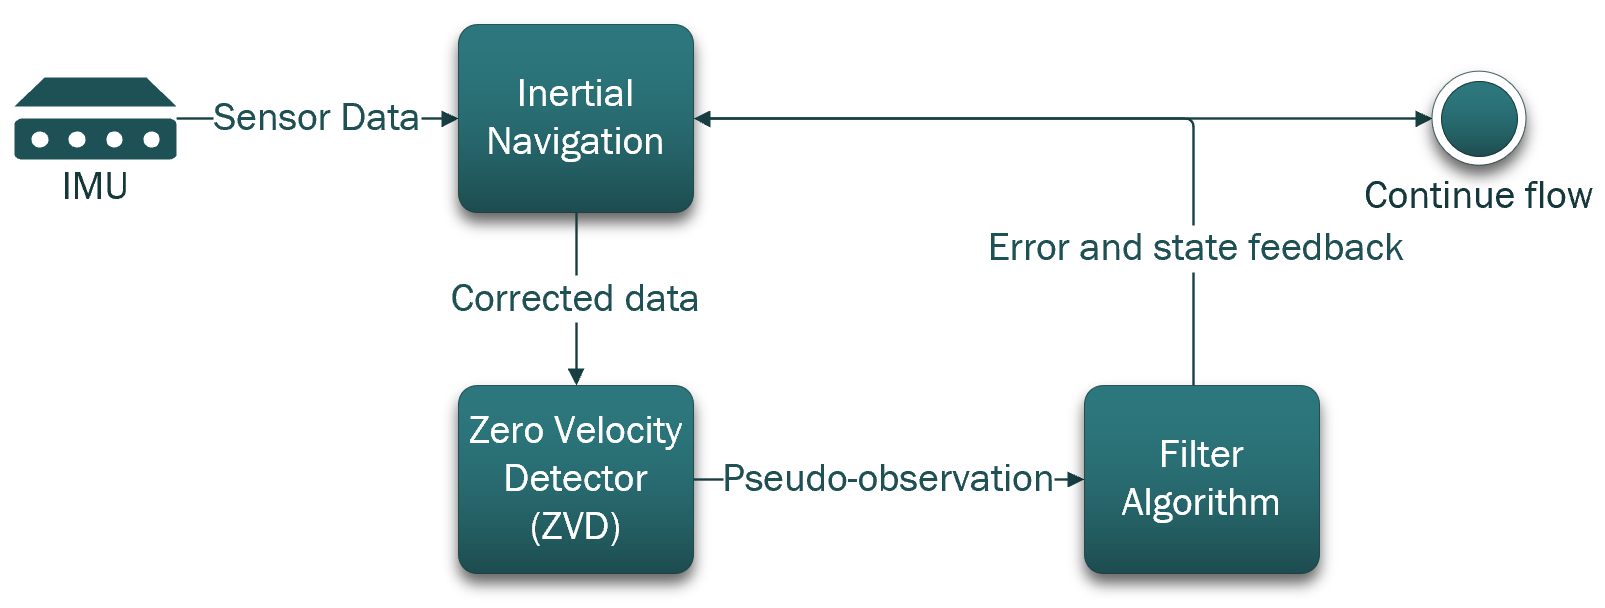
\includegraphics[width=\textwidth]{TESIS/imagenes/chap04/zero-velocity.PNG}
\caption{ Flujo de detección de velocidad cero (ZVD) de PARKIBIP.}
\label{fig:zero-velocity}
\end{figure}

\noindent Cuando el ZVD decide que el IMU se encuentra estacionario, el sistema genera una pseudo-observación y emite un evento hacia el algoritmo de filtrado del detector. El filtro compara la pseudo-observación con la estimación de velocidad del INS y usa la diferencia para estimar los errores del INS. Las estimaciones de error se retroalimentan para reducir el error acumulativo.

Luego, detectados los momentos de cero velocidad, es trivial inferir que los algoritmos ZVD´s permiten reconocer las transiciones de fases dentro del ciclo de la marcha. Por ejemplo, un ciclo binario Stance|Swing -fases de apoyo y vuelo-.

El problema de identificar los instantes de velocidad cero se formaliza como un problema de test binario de hipótesis -$H_0:$ hipótesis nula, $H_1:$ hipótesis alternativa-, y se analiza aplicando la teoría de detección estadística. Algunos ejemplos de algoritmos de ZVD son: (i) Acceleration moving variance detector -MV-, (ii) Acceleration magnitude detector -MAG-, (iii) Angular rate energy  detector (ARE), Generalized Likelihood Ratio Test -GLRT-, entre otros.

Por lo tanto, se propone la utilización de algoritmos de ZVD para romper la deriva del error cúbico mediante la técnica de ZUPT e inferir el ciclo de la marcha del sujeto en deambulación. Además, se enfatiza en el requerimiento online del sistema PARKIBIP, acentuando la complejidad de la solución. Para ello, se construirá una combinación estandarizada de algoritmos óptimos en su función (e.g. Kalman Filter, Orientation Filter, ZVD, otros algoritmos auxiliares), cuya sinergia incremente la operativa de PARKIBIP y habilite a cumplir los propósitos de dicho INS.

\section{Filtro de Kalman}\label{section:kalman-filter}

Un método de filtrado lineal de gran utilidad y con variadas aplicaciones, es el \gls{kalman-filter} (KF, por sus siglas en inglés) en sus diversas variedades. En estadística y teoría de control, el KF, también conocido como estimación cuadrática lineal (LQE), es un algoritmo que utiliza una serie de mediciones observadas a lo largo del tiempo -que contienen ruido estadístico y otras inexactitudes-, y produce estimaciones de variables desconocidas que tienden a ser más precisas que los basados en una sola medición. Suponiendo fuentes de ruido distribuidas como variables aleatorias gaussianas, el filtro de Kalman proporciona la solución que minimiza el error cuadrático medio (MMSE) del problema lineal pre-establecido.

En otras palabras, KF es un algoritmo óptimo de estimación que permite hallar la mejor estimación de variables de interés -no medibles- a partir de la combinación de variables indirectas -medibles-. De esta manera, se logra extraer información respecto a algo que no es posible medir, desde algo que si lo es.

Con la finalidad de introducir a la temática se mencionan brevemente algunas de sus aplicaciones. Los filtros de Kalman o su variación extendida para sistemas no lineales, son de gran utilidad en la robótica dado que facilitan el problema de la planificación de un camino mínimo. Un clásico problema de la navegación robótica que puede ser resuelto con dicho algoritmo, es planificar el movimiento de un robot que viaja con una velocidad limitada, desde un determinado punto a otro en una superficie en presencia de obstáculos en movimiento \cite{Nasir2017}.
\noindent Otra aplicación es lo que se denomina control y navegación de vehículos, en particular aviones, naves espaciales y barcos posicionados dinámicamente \cite{Mao2007}. Además, KF es un concepto ampliamente aplicado en el análisis de series de tiempo que se utiliza en campos como el procesamiento de señales y la econometría.

Para entrar en contexto con la utilidad de KF en PARKIBIP, se expone el problema de un sistema de navegación de un automóvil en movimiento, al estimar la posición del mismo dentro de un túnel. El automóvil integra dispositivos de medición a bordo, como lo son un IMU (acelerómetro y giroscopio) y un GPS (estima la posición en base a señales satélitales).
\noindent Dentro del túnel, el sensor de GPS se ve afectado por el bloqueo de señal satélital (e.g. señal intermitente y de baja frecuencia, ruido en el receptor). Análogamente, realizar la doble integración de la señal del acelerómetro recibida desde el IMU -para obtener la posición-, se encuentra sujeta a desvíos incrementales debido al error acumulativo de integración respecto al tiempo. 
\noindent Por lo tanto, los dispositivos de medición a bordo no logran estimar la posición por si solos. En éste escenario, un KF puede ser usado para fusionar las mediciones de los sensores y hallar la solución óptima al problema de estimar la posición del vehículo en su sistema de navegación.

\begin{figure}[H]
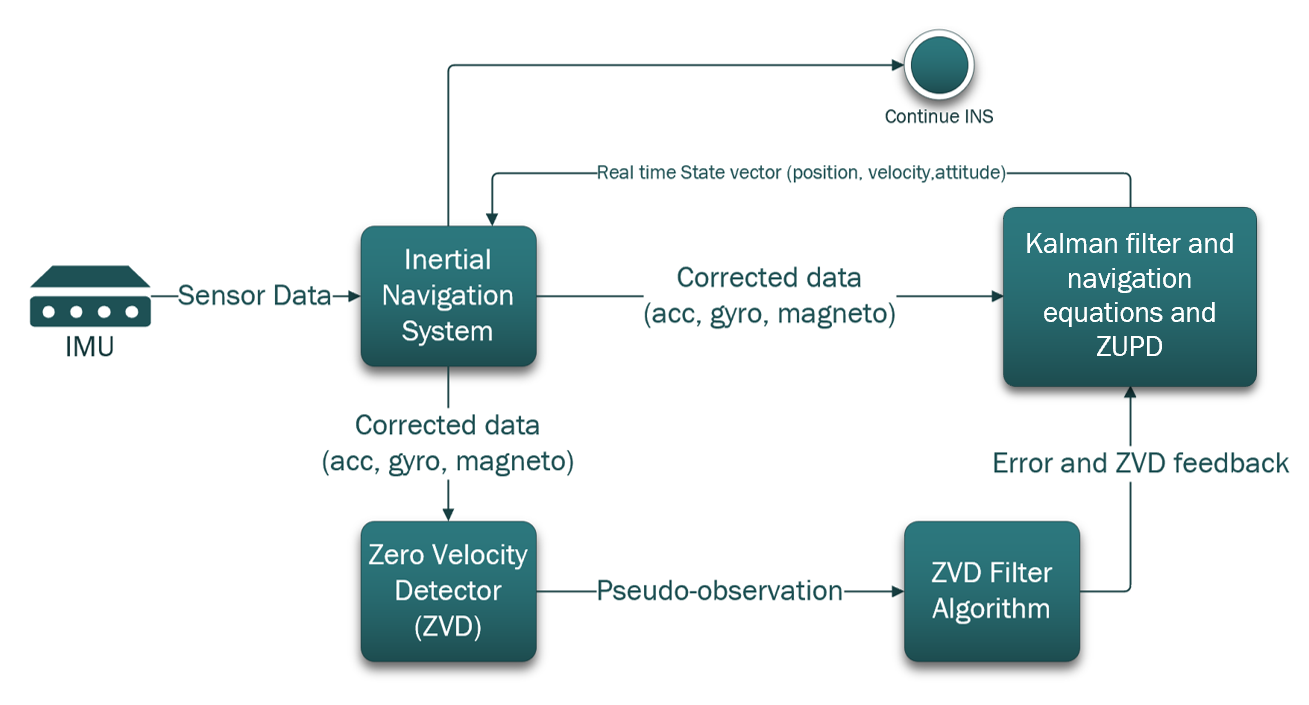
\includegraphics[width=\textwidth]{TESIS/imagenes/chap04/zero-velocity-kalman.PNG}
\caption{ Flujo de filtro de Kalman para estimar las variables indirectas posición, velocidad, altitud de un IMU en movimiento en PARKIBIP. Además, integra la compensación de actualizaciones de velocidad cero (ZUPD) mediante la fusión de un algoritmo de detección de velocidad cero (ZVD).}
\label{fig:zero-velocity-kalman}
\end{figure}

En estas condiciones, PARKIBIP empleará el filtro de Kalman para predecir en tiempo real las variables indirectas velocidad, posición y altitud (variables no medibles por un IMU) a partir de las mediciones de acelerómetro, giroscopio y magnetómetro. Asimismo, otra entrada al algoritmo, serán los momentos de cero velocidad detectados por el algoritmo de ZVD, que permitirán aplicar el ZUPT dentro del filtro de Kalman para compensar y mejorar aun mas la solución de navegación. El filtro de Kalman no solo estima el error de velocidad en los intervalos ZUPT detectados, sino que también estima las correcciones de posición, altitud, y ruido de los sensores inerciales debido a correlaciones cruzadas en la matriz de transición. La figura Fig. \ref{fig:zero-velocity-kalman} brinda un modelo de flujo de aplicación que integra los conceptos mencionados.

\section{Desarrollo de una aplicación móvil PARKIBIP}

Dentro de las expectativas funcionales del proyecto PARKIBIP se encuentra la de brindar una herramienta tecnológica que le permita a los pacientes con la enfermedad de Parkinson una rehabilitación personal; que en la actualidad es inexistente. Asimismo, se espera que dicha herramienta sea un soporte para el terapeuta al momento de tomar decisiones y evaluar al sujeto afectado. De esta manera, se logra una evaluación clínica mas objetiva, que de otra forma se hace dificultosa debido a una serie de limitaciones estructurales, logísticas y financieras.

En la actualidad, los sistemas de análisis de movimiento ópticos basados en cámaras (3D-GA) son reconocidos como el estándar de oro en la medición del movimiento. Sin embargo, requieren ejecutar las pruebas en un entorno de laboratorio con equipos de alto costo, solo se pueden usar para evaluar segmentos cortos de la marcha, requiere personal especializado, equipo considerable -i.e. laboratorio de marcha-, tiempo y sobretodo una gran inversión.

Por consiguiente, se quiere implementar un instrumento portable, accesible y de bajo costo; cuyo usuario final sea un Terapeuta y/o un Parkinsoniano. Primero, mencionado en la sección \nameref{seleccion_tecnologica}, se optó por un dispositivo que cumpla los requerimientos antedichos y sea de gran amigabilidad para su portador (i.e. pequeño, cómodo, portable). Luego, se requiere un elemento de hardware que permita interoperar con el dispositivo, procesar información y presentar resultados al usuario. 

En la actualidad, prácticamente todas las personas cuentan con dispositivos inteligentes personales con los cuales interactúan todo el día en sus tareas cotidianas. Aquí, es donde nace una gran oportunidad para PARKIBIP de combinar la tecnología IMU con los teléfonos inteligentes, aprovechando todo su potencial:

\begin{itemize}
    \item Permite una comunicación directa y personalizada hacia el usuario
    \item Ofrece atención continua (i.e. apps están disponibles 24x7)
    \item Usabilidad. Es una tecnología conocida, el desafío central es la amigabilidad en el diseño hacia el usuario.
    \item Acceso a periféricos del dispositivo. Por ejemplo el Bluetooth, requisito para enlazar a un IMU
    \item Dispositivo de procesamiento (variando el rendimiento según las características del mismo) 
\end{itemize}

Finalmente, en consideración de las necesidades de PARKIBIP y los beneficios mencionados, se propone la implementación de una aplicación móvil adecuada para el usuario final (conceptos como usabilidad, rendimiento y automatización).

\newpage

\section{Sistema operativo y lenguaje utilizado}

% Android 
La implementación del Software PARKIBIP consistió principalmente en el desarrollo de una aplicación móvil. Una decisión clave para el proyecto fue decidir el sistema operativo a emplear, en el cual se desarrolló esta aplicación. Según la herramienta StatCounter (© 1999-2020 StatCounter), la cual permite consultar estadísticas globales sobre el uso de dispositivos móviles, los dos sistemas operativos dominantes en la industria son Android (70.68\%) y iOS (28.79\%), sumando un total del 99.47\% del mercado entre estas dos plataformas.

\begin{figure}[H]
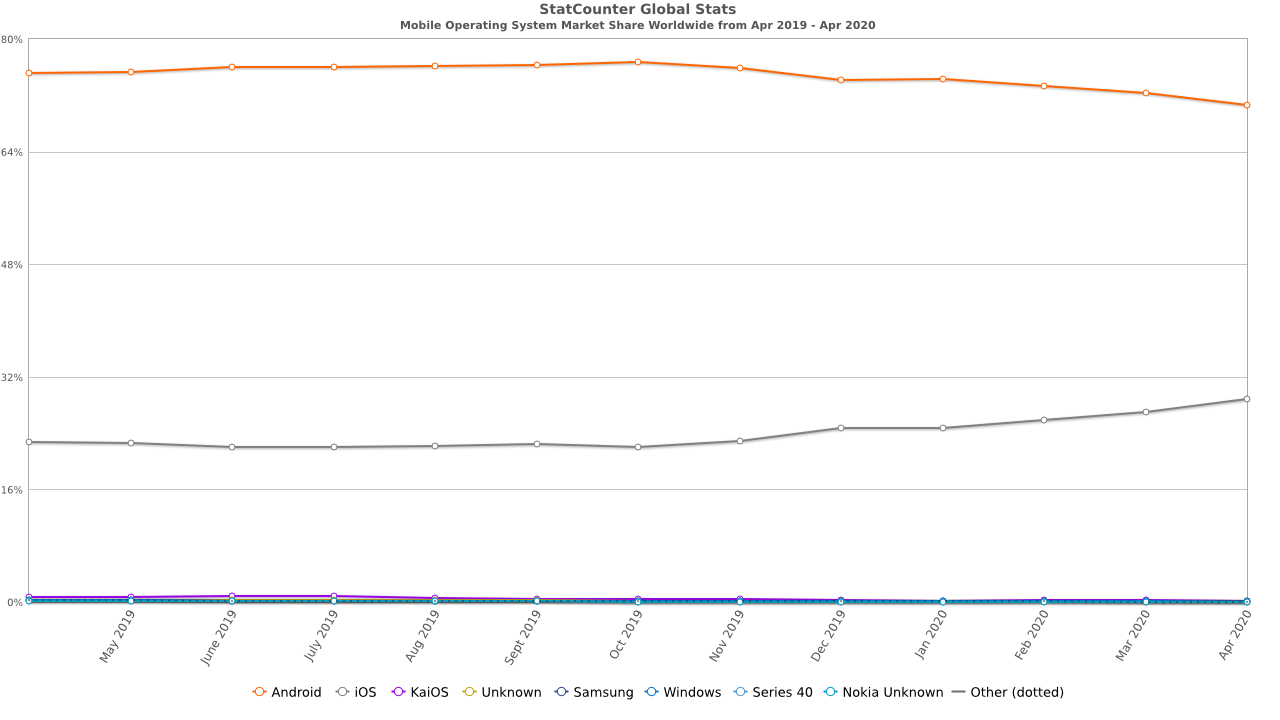
\includegraphics[width=\textwidth]{TESIS/imagenes/chap04/StatCounter-os_combined-ww-monthly-201904-202004.png}
\caption{ Evolución global de sistemas operativos en dispositivos móviles desde 04.2019 a 04.2020 \cite{StatCounter} }
\label{fig:ww-mobile-so}
\end{figure}

Uruguay no es la excepción, en donde Android es aún más dominante con respecto al resto de los sistemas operativos. En la figura Fig. \ref{fig:uy-mobile-so} se puede observar que el 85.41\% de los dispositivos móviles de Uruguay contienen un sistema operativo Android, tan solo un 14.39\% utiliza el sistema iOS y un 0.02\% ejecuta uno diferente. 

\begin{figure}[H]
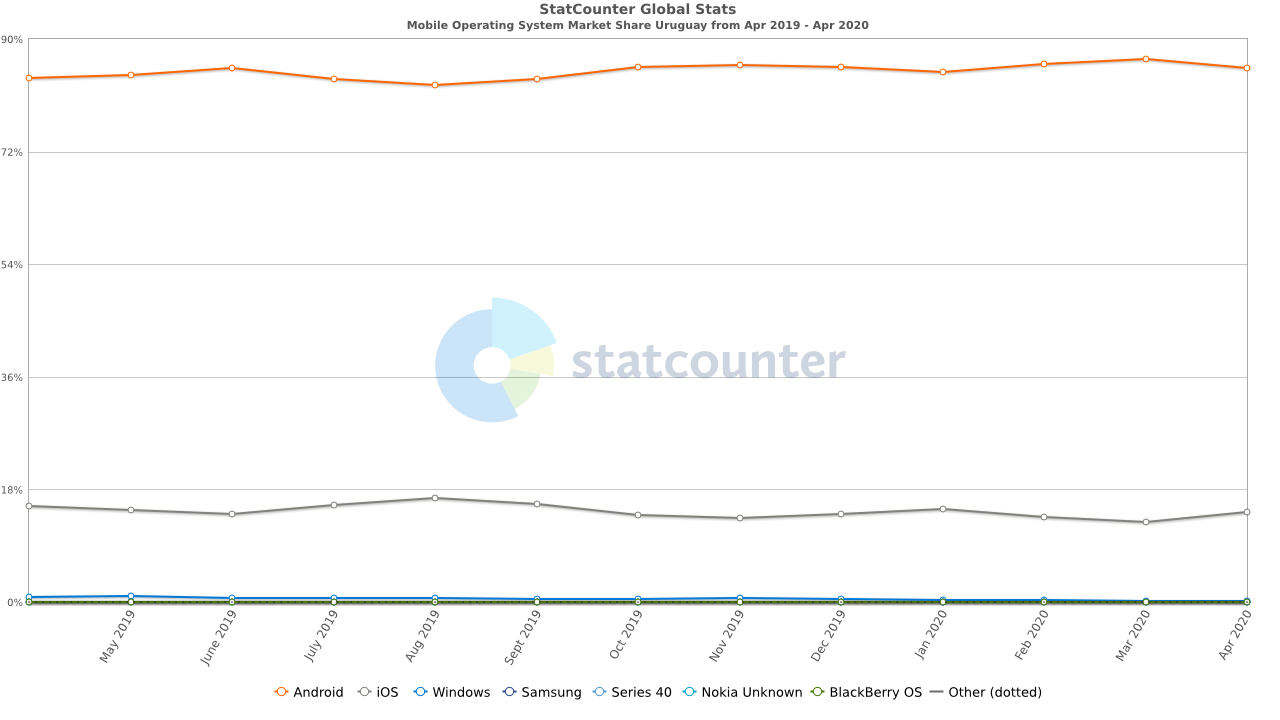
\includegraphics[width=\textwidth]{TESIS/imagenes/chap04/StatCounter-os_combined-UY-monthly-201904-202004.png}
\caption{ Sistemas operativos empleados en dispositivos móviles en Uruguay -periodo 04.2019 a 04.2020- \cite{StatCounter} }
\label{fig:uy-mobile-so}
\end{figure}

Con el objetivo de realizar un sistema más accesible para los usuarios, se decidió desarrollar la aplicación para la plataforma Android. Sin embargo, existen diversas tecnologías para el desarrollo de aplicaciones multiplataforma -que luego pueden ser soportadas por ambos sistemas operativos- (p.ej: Flutter, Xamarin, Genexus, etc.). Además, la comunidad de soporte para el uso del dispositivo de medición seleccionado existe para los lenguajes nativos de Android -Java o Kotlin-, lo que facilita la implementación y la solución de inconvenientes durante el desarrollo de la aplicación móvil, sobre todo para la interoperabilidad de la misma con el dispositivo de medición inercial.  

\section{Interfaz y experiencia de usuario (UI \& UX)}

% UX & UI 
En la última década, la ``experiencia de usuario'' (UX) se convirtió en una palabra de gran importancia en el campo de la interacción humano-computadora (HCI) y el diseño de interacción. A medida que la tecnología maduró, los productos interactivos se volvieron no solo más útiles y utilizables, sino también más modernos y fascinantes \cite{Hassenzahl2006}. Se puede decir entonces, que la experiencia de usuario no es nada más ni nada menos que cómo se siente el usuario al interactuar con un sistema de software. 

% Cualidades del software que se buscan con UI & UX 
En el área de desarrollo de aplicaciones móviles, la definición de la interfaz de usuario (UI) y la forma en que se va a interactuar con dicha aplicación es una etapa fundamental. El diseño de la interfaz de usuario debe tener en cuenta el público objetivo de dicha aplicación, para que el resultado final sea entendible y accesible para dicho público. 

% Material Design
Por lo tanto, a fin de generar un buen diseño de la interfaz de usuario (UI) se deben seguir los lineamientos de diseño que la plataforma sugiere, ya que el usuario de ese dispositivo estará familiarizado con dichos lineamientos. En este sentido, la plataforma Android ofrece una guía de diseño llamada ``Material Design'', utilizada por la gran mayoría de las aplicaciones disponibles en la plataforma. Material Design, es un conjunto de guías, componentes y herramientas que engloban las mejores practicas de diseño de UI para Android \cite{MaterialDesign}. 
 
% Sketch 
En PARKIBIP, se utilizó Material Design para diseñar tanto la interfaz de usuario como la experiencia de usuario. Para esto, se empleo la herramienta de diseño gráfico y prototipado Sketch (© 2020 Sketch B.V.). Sketch es un editor de vectores gráficos funcional en macOS, desarrollado por la empresa holandesa Boheamian Coding. Es utilizada para el diseño de UI y UX por más de un millón de usuarios en todo el mundo. Además, tiene funcionalidades para prototipado de aplicaciones y colaboración. 

\section{Especificación detallada y alcance del proyecto }
\label{chap:project-scope}

% Objetivo del producto
El presente proyecto tiene como objetivo la implementación de PARKIBIP, un sistema que le brinde soporte a la toma de decisiones de un terapeuta y a su vez, le permita a los pacientes con la enfermedad de Parkinson una rehabilitación personal. Durante las sesiones de fisioterapia los estímulos externos pueden mejorar las características de la marcha. PARKIBIP entonces busca emular estos estímulos en tiempo real para permitirle al enfermo una rehabilitación personal que prolongue el trabajo del fisioterapeuta en su vida cotidiana. Es decir, reeducar al paciente en rehabilitación mediante feedback -estímulos adecuados y repetitivos- a manipular eventos fisiológicos no detectados de forma voluntaria, logrando una función terapéutica.

Por lo tanto, integrando los avances en dispositivos de análisis de la marcha con los teléfonos inteligentes de uso cotidiano, haciendo uso de la evidencia adquirida a lo largo del tiempo en las terapias de Biofeedback para lograr construir un sistema portable -uso cotidiano y en exteriores-, accesible y de bajo costo; cuyo objetivo sea aumentar el control voluntario sobre los procesos fisiológicos. Mediante un dispositivo electrónico vestible de bajo costo (IMU - Unidad de Medición Inercial), que combina múltiples sensores (p. ej. acelerómetro, giroscopio, magnetómetro, entre otros), se particiona el ciclo de marcha del usuario permitiendo identificar distintos eventos, tales como, el contacto inicial con el suelo o la fase de vuelo. Finalmente, con los eventos detectados, se aplican ciertos algoritmos matemáticos que calculan los parámetros espacio temporales claves, y en base a un módulo clínico se estimula adecuadamente al usuario.

% Alcance
Definir el alcance del proyecto es una actividad central dentro del proceso de planeación del proyecto -también denominada ingeniería de requisitos-, que implica determinar y documentar una lista de objetivos finales, entregables y tareas específicas del proyecto. En otras palabras, es el trabajo a realizar, son las características y funcionalidades que caracterizan un producto, servicio o resultado; define los límites del proyecto, qué características se incluirán e implementarán dentro del mismo. 

En software, es habitual definir el alcance de un proyecto mediante la especificación de requisitos de software (SRS, del ingles Software Requirements Specification), siendo una descripción de un sistema a desarrollar. La SRS establece requisitos funcionales y no funcionales y en general incluye un conjunto de historias de usuario o casos de uso que el sistema debe proporcionar. 

% Historias de usuario
Una herramienta fundamental para definir el alcance de un trabajo es la historia de usuario, que debe ser completada para cumplir con los requisitos de una funcionalidad del producto o un objetivo del usuario de forma que la misma le brinde un valor particular. Es la unidad de trabajo más pequeña en un marco de desarrollo ágil y se encuentra expresado desde la perspectiva del usuario del software. Es decir, una historia de usuario es una explicación general e informal de una funcionalidad del sistema, escrita desde la perspectiva del usuario final en lenguaje natural. Asimismo, una Épica es una unidad de alto nivel que contiene o desglosa un conjunto de tareas más pequeñas (historias de usuario).

Por lo tanto, se optó por construir la especificación de PARKIBIP en base a la definición de historias de usuarios, y por consiguiente su conjunto es el alcance de la solución. Algunas de los beneficios adicionales contemplados para emplear esta metodología fueron:

\begin{itemize}
    \item Una lista de tareas pendientes mantiene al equipo centrado en tareas que deben completarse, sin embargo un conjunto de historias lo mantiene centrado en solucionar problemas para el usuario final.
    \item Con el objetivo definido en historias, el equipo puede colaborar para decidir cómo implementar la mejor solución, dividir las tareas y cumplir con dicho objetivo.
    \item Las historias fomentan que el equipo piense de forma crítica y creativa sobre cómo lograr mejor un objetivo.
    \item Con cada historia el equipo de desarrollo realiza pequeños incrementos hacia el producto final y disfruta pequeños logros, lo que aumenta la motivación.
\end{itemize}

A continuación, se lista el conjunto de historias de usuario de PARKIBIP junto a sus actores, épica, descripción y nombre descriptivo. Cabe resaltar que el hecho de incluir la Épica y su desglose en historias, permite especificar de forma adicional el WBS  (del ingles, Work Breakdown Structure) del proyecto PARKIBIP. La nomenclatura de especificación para cada historia de usuario es: Como $<Rol>$ se Desea $<Objetivo>$ Para $<Beneficio>$.

\begin{table}[H] 
\centering
\begin{tabular}{| p{2cm} | p{10cm} |}
\hline
Épica & Usuario\\ \hline
Nombre & Autenticación y manejo de Sesión\\ \hline
Actores & Terapeuta | Paciente\\ \hline
Descripción &  Como Terapeuta o Paciente previamente registrado se desea acceder al sistema PARKIBIP. Para esto ingresará sus credenciales de acceso y el sistema realizará la validación y autorización correspondiente.\\ \hline
\end{tabular}
\end{table}

\begin{table}[H] 
\centering
\begin{tabular}{|p{2cm} | p{10cm} |}
\hline
Épica & Usuario\\ \hline
Nombre & Gestión de Roles y Permisos de Usuarios\\ \hline
Actores & PARKIBIP\\ \hline
Descripción &  Como Sistema se quiere distinguir a los Usuarios por su Rol. PARKIBIP podrá determinar la información y las funcionalidades que le son permitidas según el Rol del usuario activo y sus autorizaciones asociadas.\\ \hline
\end{tabular}
\end{table}

\begin{table}[H] 
\centering
\begin{tabular}{| p{2cm} | p{10cm} |}
\hline
Épica & Usuario\\ \hline
Nombre & Visualización de Usuario activo discriminado por Rol\\ \hline
Actores & Terapeuta | Paciente\\ \hline
Descripción &  Como Terapeuta o Paciente se quiere visualizar su información de usuario en el Sistema.\\ \hline
\end{tabular}
\end{table}

\begin{table}[H] 
\centering
\begin{tabular}{| p{2cm} | p{10cm} |}
\hline
Épica & IMU\\ \hline
Nombre & Escaneo de dispositivos Bluetooth\\ \hline
Actores & Terapeuta | Paciente\\ \hline
Descripción & Como Terapeuta o Paciente se desea identificar los dispositivos IMU en su radio cercano, y así iniciar las configuraciones pertinentes para su uso.\\ \hline
\end{tabular}
\end{table}

\begin{table}[H] 
\centering
\begin{tabular}{| p{2cm} | p{10cm} |}
\hline
Épica & IMU\\ \hline
Nombre & Emparejamiento y sincronización de Dispositivo IMU\\ \hline
Actores & Terapeuta | Paciente\\ \hline
Descripción &  Como Terapeuta o Paciente se quiere emparejar un dispositivo IMU previamente escaneado por PARKIBIP, conforme a iniciar sesiones de rehabilitación.\\ \hline
\end{tabular}
\end{table}

\begin{table}[H] 
\centering
\begin{tabular}{| p{2cm} | p{10cm} |}
\hline
Épica & IMU\\ \hline
Nombre & Establecer sensor de color LED de luz\\ \hline
Actores & PARKIBIP\\ \hline
Descripción &  Como Sistema se desea configurar el indicador LED de luz de un dispositivo previamente conectado. De esta manera, se logra distinguir visualmente -en la interfaz gráfica y en el cuerpo del paciente- el dispositivo conectado a cuál extremidad.\\ \hline
\end{tabular}
\end{table}

\begin{table}[H] 
\centering
\begin{tabular}{| p{2cm} | p{10cm} |}
\hline
Épica & IMU\\ \hline
Nombre & Establecer la tasa de datos de salida y el rango de datos del Sensor Acelerómetro\\ \hline
Actores & PARKIBIP\\ \hline
Descripción & Como Sistema se quiere establecer la frecuencia en Hz de recolección de datos y el rango posible de datos para el sensor Acelerómetro de un IMU sincronizado.  \\ \hline
\end{tabular}
\end{table}

\begin{table}[H] 
\centering
\begin{tabular}{| p{2cm} | p{10cm} |}
\hline
Épica & IMU\\ \hline
Nombre & Establecer la tasa de datos de salida y el rango de datos del Sensor Giroscopio\\ \hline
Actores & PARKIBIP\\ \hline
Descripción & Como Sistema se quiere establecer la frecuencia en Hz de recolección de datos y el rango posible de datos para el sensor Giroscopio de un IMU sincronizado.\\ \hline
\end{tabular}
\end{table}

\begin{table}[H] 
\centering
\begin{tabular}{| p{2cm} | p{10cm} |}
\hline
Épica & IMU\\ \hline
Nombre & Establecer el rango de datos,  ruido, corriente media del Sensor Magnetómetro\\ \hline
Actores & PARKIBIP\\ \hline
Descripción & Como Sistema se quiere establecer la frecuencia en Hz de recolección de datos, el ruido y la corriente media para el sensor Magnetómetro de un IMU sincronizado.\\ \hline
\end{tabular}
\end{table}

\begin{table}[H] 
\centering
\begin{tabular}{| p{2cm} | p{10cm} |}
\hline
Épica & IMU\\ \hline
Nombre & Iniciar recolección asincónica de datos por sensor en un IMU\\ \hline
Actores & PARKIBIP\\ \hline
Descripción &  Como Sistema se quiere iniciar la recolección de datos crudos por tipo de sensor para un IMU previamente conectado. De acuerdo a las necesidades numéricas, el sistema será capaz de iniciar cada sensor correspondiente para un procesamiento posterior de datos.\\ \hline
\end{tabular} 
\end{table}

\begin{table}[H] 
\centering
\begin{tabular}{| p{2cm} | p{10cm} |}
\hline
Épica & IMU\\ \hline
Nombre & Detener recolección asincónica de datos por sensor en un IMU\\ \hline
Actores & PARKIBIP\\ \hline
Descripción &  Como Sistema se quiere detener la recolección de datos crudos por tipo de sensor para un sensor activo en un IMU previamente conectado. De esta manera, se liberan los recursos asignados en el IMU y en el Host para una posterior recolección.\\ \hline
\end{tabular}
\end{table}

\begin{table}[H] 
\centering
\begin{tabular}{| p{2cm} | p{10cm} |}
\hline
Épica & IMU\\ \hline
Nombre & Empaquetado de datos de múltiples sensores de un dispositivo IMU\\ \hline
Actores & PARKIBIP\\ \hline
Descripción & Como Sistema se quiere consolidar los diferentes datos recolectados (acelerómetro, giroscopio, magnetómetro) en un único paquete de datos con Timestamp de referencia. El requerimiento de manejar tantos threads como sensores activos, que a su vez tienen frecuencias distintas, incrementa la complejidad de empaquetado de datos. PARKIBIP debe implementar un algoritmo de empaquetado de datos consistente a las distintas frecuencias. \\ \hline
\end{tabular}
\end{table}

\begin{table}[H] 
\centering
\begin{tabular}{| p{2cm} | p{10cm} |}
\hline
Épica & IMU\\ \hline
Nombre & Administrar conexiones por dispositivo IMU\\ \hline
Actores & PARKIBIP\\ \hline
Descripción & Como Sistema se desea gestionar las diferentes conexiones a los múltiples dispositivos conectados, y así intercambiar distintos comandos con el IMU adecuado.\\ \hline
\end{tabular}
\end{table}

\begin{table}[H] 
\centering
\begin{tabular}{| p{2cm} | p{10cm} |}
\hline
Épica & IMU\\ \hline
Nombre & Establecer modulo de vibración IMU\\ \hline
Actores & PARKIBIP\\ \hline
Descripción &  Como Sistema se quiere configurar el motor vibratorio integrado al IMU, establecer la duración e intensidad de vibración. Siendo el presente modulo uno de los estímulos externos base a emplear en PARKIBIP.\\ \hline
\end{tabular}
\end{table}

\begin{table}[H] 
\centering
\begin{tabular}{| p{2cm} | p{10cm} |}
\hline
Épica & Configuración\\ \hline
Nombre & Visualización de parámetros y constantes Generales\\ \hline
Actores & Terapeuta | Paciente\\ \hline
Descripción & Como Terapeuta o Paciente se quiere visualizar parámetros generales de fabrica para evaluar dinámicamente su uso en una sesión de rehabilitación. \\ \hline
\end{tabular}
\end{table}

\begin{table}[H] 
\centering
\begin{tabular}{| p{2cm} | p{10cm} |}
\hline
Épica & Configuración\\ \hline
Nombre & Visualización de parámetros y constantes específicos por Método numérico\\ \hline
Actores & Terapeuta | Paciente\\ \hline
Descripción & Como Terapeuta o Paciente se quiere visualizar información de parámetros específicos por algoritmos.  \\ \hline
\end{tabular}
\end{table}

\begin{table}[H] 
\centering
\begin{tabular}{| p{2cm} | p{10cm} |}
\hline
Épica & Configuración\\ \hline
Nombre & Modificación de parámetros y constantes\\ \hline
Actores & Terapeuta | Paciente\\ \hline
Descripción & Como Terapeuta o Paciente se quiere actualizar parámetros generales y específicos de algoritmos. Permitiendo afinar el comportamiento del algoritmo elegido según las necesidades clínicas del paciente en rehabilitación. \\ \hline
\end{tabular}
\end{table}

\begin{table}[H] 
\centering
\begin{tabular}{| p{2cm} | p{10cm} |}
\hline
Épica & Configuración\\ \hline
Nombre & Restablecer valores de parámetros y constantes\\ \hline
Actores & Terapeuta | Paciente\\ \hline
Descripción & Como Terapeuta o Paciente se desea actualizar los parámetros generales y específicos de algoritmos a sus valores de fabrica elegidos como óptimos por los desarrolladores. \\ \hline
\end{tabular}
\end{table}

\begin{table}[H] 
\centering
\begin{tabular}{| p{2cm} | p{10cm} |}
\hline
Épica & Configuración\\ \hline
Nombre & Deshacer cambios de parámetros y constantes\\ \hline
Actores & Terapeuta | Paciente\\ \hline
Descripción & Como Terapeuta o Paciente se desea deshacer cambios involuntarios de parámetros, retornando a la configuración previa. \\ \hline
\end{tabular}
\end{table}

\begin{table}[H] 
\centering
\begin{tabular}{| p{2cm} | p{10cm} |}
\hline
Épica & Paciente\\ \hline
Nombre & Alta de Pacientes\\ \hline
Actores & Terapeuta\\ \hline
Descripción & Como Terapeuta se quiere dar de alta Pacientes para que puedan participar de sesiones de rehabilitación. \\ \hline
\end{tabular}
\end{table}

\begin{table}[H] 
\centering
\begin{tabular}{| p{2cm} | p{10cm} |}
\hline
Épica & Paciente\\ \hline
Nombre & Visualización y listado de Pacientes\\ \hline
Actores & Terapeuta\\ \hline
Descripción & Como Terapeuta se desea visualizar la plantilla de Pacientes junto a su información básica. \\ \hline
\end{tabular}
\end{table}

\begin{table}[H] 
\centering
\begin{tabular}{| p{2cm} | p{10cm} |}
\hline
Épica & Paciente\\ \hline
Nombre & Búsqueda y filtrado de Pacientes\\ \hline
Actores & Terapeuta\\ \hline
Descripción &  Como Terapeuta se desea buscar de forma amigable un Paciente mediante filtros conforme a seleccionarlo como usuario activo de Sesiones de rehabilitación.\\ \hline
\end{tabular}
\end{table}

\begin{table}[H] 
\centering
\begin{tabular}{| p{2cm} | p{10cm} |}
\hline
Épica & Paciente\\ \hline
Nombre & Selección de Paciente activo\\ \hline
Actores & Terapeuta\\ \hline
Descripción &  Como Terapeuta, visualizando el listado de Pacientes y haciendo uso del buscador, podrá establecer un Paciente como Usuario activo. El Sistema reconocerá automáticamente al Usuario activo como el participante de una Sesión de rehabilitación.\\ \hline
\end{tabular}
\end{table}

\begin{table}[H] 
\centering
\begin{tabular}{| p{2cm} | p{10cm} |}
\hline
Épica & Paciente\\ \hline
Nombre & Recuperación de último Estado de Sistema\\ \hline
Actores & PARKIBIP\\ \hline
Descripción &  Como Sistema se quiere facilitar y automatizar toda característica de Parkibip de forma que se minimice la selección/digitación por parte del usuario de PARKIBIP. Para ello, el Sistema mantendrá distintos Estados de la aplicación y será capaz de almacenar y recuperar su ultimo Estado (p. ej. Paciente activo, Usuario Logueado, Configuraciones, etc.) \\ \hline
\end{tabular}
\end{table}

\begin{table}[H] 
\centering
\begin{tabular}{| p{2cm} | p{10cm} |}
\hline
Épica & Sesión\\ \hline
Nombre & Visualización e Historial de Sesiones \\ \hline
Actores & Terapeuta | Paciente\\ \hline
Descripción & Como Terapeuta o Paciente se desea visualizar el Historial de Sesiones de rehabilitación ordenadas de forma descendente por cada fecha de realización. El listado permitirá ver información básica de la Sesión y navegar a su información mas detallada. \\ \hline
\end{tabular}
\end{table}

\begin{table}[H] 
\centering
\begin{tabular}{| p{2cm} | p{10cm} |}
\hline
Épica & Sesión\\ \hline
Nombre & Búsqueda y filtrado de Sesiones históricas\\ \hline
Actores & Terapeuta | Paciente\\ \hline
Descripción & Como Terapeuta o Paciente se desea buscar de forma amigable cada Sesión dentro del Historial de Sesiones mediante filtros, y así obtener información detallada según necesidad del usuario. \\ \hline
\end{tabular}
\end{table}

\begin{table}[H] 
\centering
\begin{tabular}{| p{2cm} | p{10cm} |}
\hline
Épica & Sesión\\ \hline
Nombre & Selección de Sesión\\ \hline
Actores & Terapeuta | Paciente \\ \hline
Descripción & Como Terapeuta o Paciente se quiere obtener información particular respecto a una Sesión previamente realizada. Para ello, mediante el uso del buscador podrá filtrar las sesiones de rehabilitación e ingresar a una interfaz que presente información genérica y otra con un nivel de entendimiento técnico.\\ \hline
\end{tabular}
\end{table}

\begin{table}[H] 
\centering
\begin{tabular}{| p{2cm} | p{10cm} |}
\hline
Épica & Sesión\\ \hline
Nombre & Resumen general de Sesión\\ \hline
Actores & Terapeuta | Paciente\\ \hline
Descripción & Como Terapeuta o Paciente se desea analizar y evaluar cada Sesión de rehabilitación mediante la visualización del comportamiento de los parámetros espacio-temporales de la marcha efectuada. Algunos parámetros son: duración, cadencia, velocidad promedio e instantánea, aceleración promedio e instantánea.\\ \hline
\end{tabular}
\end{table}

\begin{table}[H] 
\centering
\begin{tabular}{| p{2cm} | p{10cm} |}
\hline
Épica & Sesión\\ \hline
Nombre & Resumen gráfico de Sesión\\ \hline
Actores & Terapeuta | Paciente\\ \hline
Descripción & Como Terapeuta o Paciente se desea analizar y evaluar cada Sesión de rehabilitación de forma gráfica  respecto al tiempo (p. ej. velocidad, trayectoria, pasos).\\ \hline
\end{tabular}
\end{table}

\begin{table}[H] 
\centering
\begin{tabular}{| p{2cm} | p{10cm} |}
\hline
Épica & Sesión activa\\ \hline
Nombre & Iniciar Sesión de Rehabilitación\\ \hline
Actores & Terapeuta | Paciente \\ \hline
Descripción & Como Terapeuta o Paciente se quiere realizar una Sesión de rehabilitación para un Paciente activo. De esta forma, con las pre-condiciones funcionales cubiertas, el Sistema identificará las fases de la marcha y estimulará de acuerdo al protocolo pre-establecido. 

El usuario de PARKIBIP, únicamente tendrá que iniciar la Sesión, luego PARKIBIP automatizará por completo el flujo de proceso necesario para cumplir el requerimiento bajo el empleo de algoritmos numéricos particulares.

Algunas de las pre-condiciones son los dispositivos conectados, paciente activo seleccionado.\\ \hline
\end{tabular}
\end{table}

\begin{table}[H] 
\centering
\begin{tabular}{| p{2cm} | p{10cm} |}
\hline
Épica & Sesión activa\\ \hline
Nombre & Detener Sesión para Paciente activo\\ \hline
Actores & Terapeuta | Paciente\\ \hline
Descripción & Como Terapeuta o Paciente  se desea detener una Sesión de rehabilitación previamente iniciada. El Sistema liberará recursos asignados -rendimiento y consumo energético de dispositivos- y presentara una interfaz con los resultados detallados de la Sesión efectuada.\\ \hline
\end{tabular}
\end{table}

\begin{table}[H] 
\centering
\begin{tabular}{| p{2cm} | p{10cm} |}
\hline
Épica & Sesión activa\\ \hline
Nombre & Partición del ciclo de la marcha\\ \hline
Actores & PARKIBIP\\ \hline
Descripción & Como Sistema se quiere detectar eficazmente y en tiempo real los eventos asociados a la partición del ciclo de la marcha de cada Paciente (p. ej. HS, TO). Mediante la recolección de datos en tiempo real de los distintos sensores del IMU, y bajo el procesamiento de algoritmos numéricos particulares (existentes o propuestos) el sistema será capaz de detectar la partición del ciclo de la marcha. 

Para ello, serán requisitos los dispositivos conectados, los sensores asociados establecidos, los dispositivos posicionados en los tobillos del paciente mediante banda elástica y una Sesión de rehabilitación activa recolectando los datos de sensores inerciales.  \\ \hline
\end{tabular}
\end{table}

\begin{table}[H] 
\centering
\begin{tabular}{| p{2cm} | p{10cm} |}
\hline
Épica & Sesión activa\\ \hline
Nombre & Identificación adecuada de estímulos en base a procesamiento de reglas\\ \hline
Actores & PARKIBIP\\ \hline
Descripción & Como Sistema se quiere automatizar la identificación adecuada de estímulos, bajo el soporte de la funcionalidad Partición del ciclo de la marcha, para lograr estimular al Paciente en rehabilitación cuando corresponda. \\ \hline
\end{tabular}
\end{table}

\begin{table}[H] 
\centering
\begin{tabular}{| p{2cm} | p{10cm} |}
\hline
Épica & Sesión activa\\ \hline
Nombre & Estimular de forma vibratoria al Paciente de acuerdo a protocolo preestablecido\\ \hline
Actores & PARKIBIP\\ \hline
Descripción &  Como Sistema se desea estimular mediante vibración el cuerpo del Paciente en rehabilitación, que se encuentra unido al dispositivo IMU durante una Sesión activa. El estimulo externo, sera el feedback que reeduque la marcha del sujeto afectado. Para ello, PARKIBIP deberá implementar un Protocolo clínico que indique el instante de estimulación externa.\\ \hline
\end{tabular}
\end{table}

\begin{table}[H] 
\centering
\begin{tabular}{| p{2cm} | p{10cm} |}
\hline
Épica & Sesión activa\\ \hline
Nombre & Estimular de forma sonora al Paciente de acuerdo a protocolo preestablecido\\ \hline
Actores & PARKIBIP\\ \hline
Descripción &  Como Sistema se desea estimular de forma sonora al Paciente en rehabilitación durante una Sesión activa. Idéntico al estimulo vibratorio, PARKIBIP deberá empleará un Protocolo clínico que indique el instante de estimulación externa.\\ \hline
\end{tabular}
\end{table}

\begin{table}[H] 
\centering
\begin{tabular}{| p{2cm} | p{10cm} |}
\hline
Épica & Sesión activa\\ \hline
Nombre & Computo de parámetros espacio-temporales de interés\\ \hline
Actores & PARKIBIP\\ \hline
Descripción & Como Sistema se desea realizar una estimación en tiempo real de los parámetros espacio-temporales de la marcha durante una sesión de rehabilitación. Mediante la recolección de datos en tiempo real de los distintos sensores del IMU, y bajo el procesamiento de algoritmos numéricos particulares (existentes o propuestos), PARKIBIP será capaz de estimar la duración, la cadencia, la velocidad, la aceleración y la cantidad de pasos en el transcurso de la Sesión. Logrando un resumen objetivo de la marcha del sujeto afectado y siendo el soporte a toma de decisiones posteriores, que de otra forma serían subjetivas.\\ \hline
\end{tabular}
\end{table}

\begin{table}[H] 
\centering
\begin{tabular}{| p{2cm} | p{10cm} |}
\hline
Épica & Biofeedback\\ \hline
Nombre & Configuración de modo de estimulo: Vibratorio y/o sonoro\\ \hline
Actores & Terapeuta | Paciente\\ \hline
Descripción & Como Terapeuta o Paciente se quiere establecer el formato de estimulación externa al Paciente en rehabilitación; con el fin de maximizar resultados en el re-aprendizaje de una marcha adecuada. \\ \hline
\end{tabular}
\end{table}

\begin{table}[H] 
\centering
\begin{tabular}{| p{2cm} | p{10cm} |}
\hline
Épica & Biofeedback\\ \hline
Nombre & Modulo de Biofeedback. Configuración de Protocolo de estimulo\\ \hline
Actores & Terapeuta\\ \hline
Descripción &  Como Terapeuta se quiere establecer un formato condicional de estímulos, bajo el desarrollo de reglas clínicas de decisión. Según las necesidades del Paciente, el protocolo indica las necesidades de estímulos para dicho sujeto, indicando el instante temporal, característica disparadora, modo de estimulo. En otras palabras, el Protocolo PARKIBIP es análogo a una receta clínica. \\ \hline
\end{tabular}
\end{table}




 % Se carga el capítulo Proyecto: Decisiones de diseño
  \chapter{Implementación} \label{chap:implementation}

% QUE 0. De que trata PARKIBIP
PARKIBIP es el resultado del trabajo de un equipo interdisciplinario, a partir de la experiencia de fisioterapeutas e ingenieros que definen las reglas para estimular a los pacientes durante la marcha de sujetos afectados por la patología de Parkinson.

PARKIBIP se basa en (i) la detección de las fases del ciclo de la marcha, (ii) el computo en tiempo real de los parámetros espacio-temporales de personas, y (iii) en base a reglas clínicas de decisión, procura estimular al paciente -en forma de vibración y/o sonora- para permitirle una rehabilitación personal que contribuya al trabajo del fisioterapeuta. En otras palabras, bajo la evidencia de las terapias de biofeedback y el trabajo de terapeutas durante sesiones de rehabilitación, se pretende reeducar la marcha del sujeto afectado mediante feedbacks adecuados. 

% QUE 1. Presentar el ciclo de la marcha de Parkibip y algunos métodos. Dar una idea al lector del flujo
Por lo tanto, para ejecutar un patrón de marcha más efectivo y estimular el proceso de aprendizaje motor se requiere identificar el ciclo de la marcha. Ya mencionado en el apartado \nameref{section:partition-cycle}, PARKIBIP se orienta a estimar la fase de apoyo y fase de vuelo por cada extremidad. Para ello, empleando algoritmos de Zero Velocity Detection, Kalman Filter y Orientation Filter; PARKIBIP se enfoca en predecir eficazmente los eventos Heel Strike y Toe Off. 

\section{Arquitectura de PARKIBIP}

Con el objetivo de enfrentar desafíos clínicos y tecnológicos específicos, PARKIBIP fue diseñado en capas. La solución tecnológica consiste en una arquitectura completamente portátil y wearable basada en Unidades de Medición Inercial (IMU), conectadas a través del protocolo Bluetooth a un teléfono inteligente Android, que funciona como una plataforma de procesamiento portátil. De esta manera, se diseñó e implemento la arquitectura de sistemas de la Fig. \ref{FIG:Arquitectura2}.

\begin{figure}[!h]
\resizebox{\textwidth}{!}{
\centering
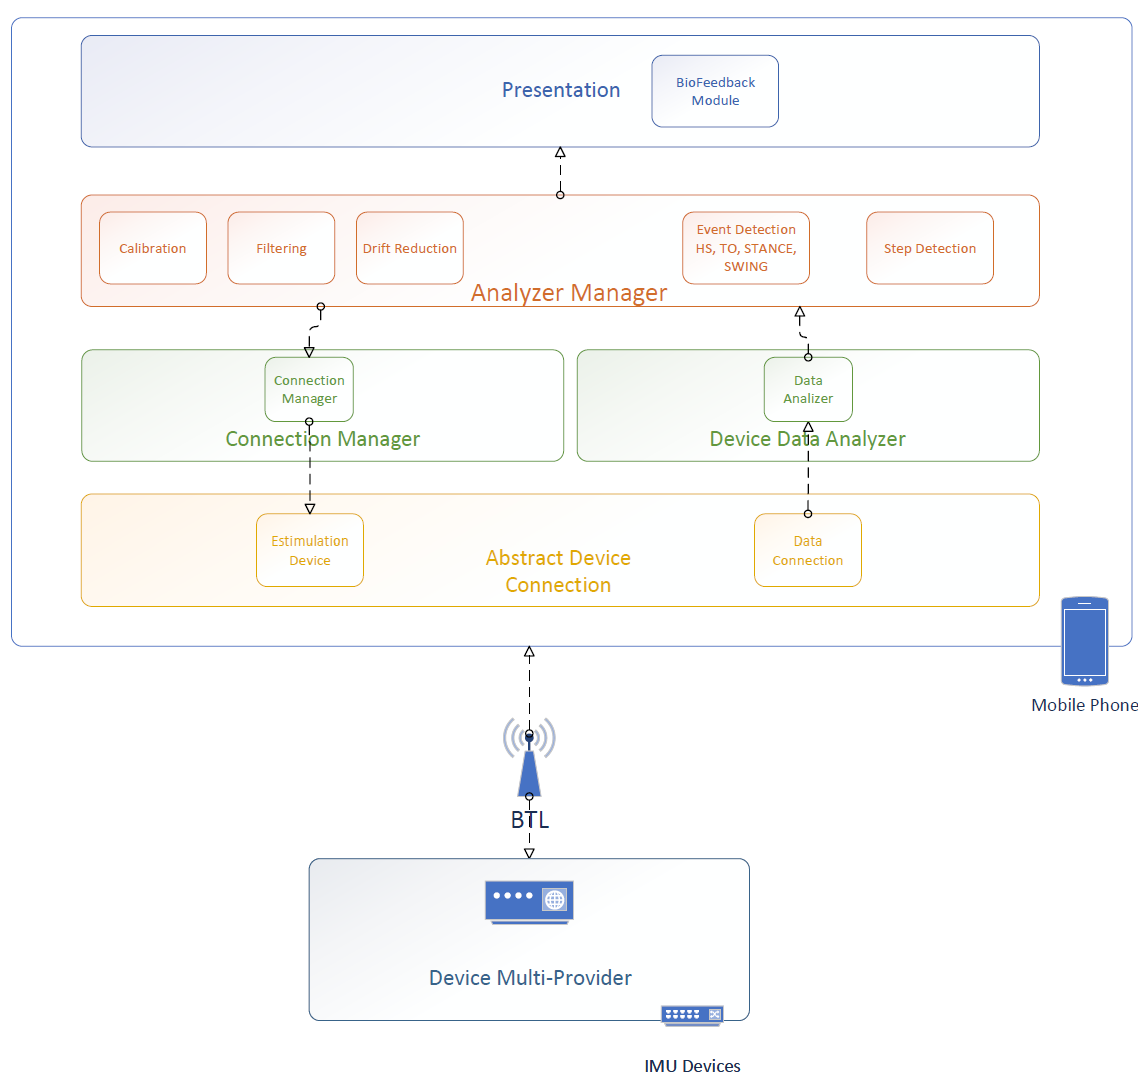
\includegraphics{TESIS/imagenes/img/Arquitectura2.png}}
\caption{Arquitectura del sistema PARKIBIP. Se compone de seis capas bien definidas desde el controlador del hardware hasta la capa de presentación. }
\label{FIG:Arquitectura2}
\end{figure}

En el diseño se pueden identificar seis capas específicas, con responsabilidades bien delineadas. Primero, y externo al Software de la aplicación Android, los dispositivos IMU con conectividad Bluetooth compuestos por los distintos sensores de movimiento. Asimismo, se identifican tres módulos de bajo nivel, vinculados a la conectividad y búsqueda, interacción con los distintos dispositivos y recuperación de datos de los sensores empleados (``Abstract Device Connection'', ``Connection manager'', ``Device Data Analizer''). Luego, se encuentra un módulo de procesamiento de la información recopilada, vinculado al análisis y aplicación de algoritmos matemáticos que identifican los parámetros espacio temporales (``Analizer Manager''). Finalmente, un módulo de presentación de resultados, compuesto por un controlador clínico capaz de tomar decisiones y estimular adecuadamente al usuario.

\section{Componentes de PARKIBIP}

El dispositivo seleccionado en \nameref{section:imu-selection}, MetaMotionR (MMR), es un dispositivo portátil que ofrece un monitoreo continuo y en tiempo real de los datos de los sensores ambientales y de movimiento. Dentro de las características principales del MMR se encuentran:
\begin{itemize}
    \item SDK (del inglés, Software Development Kit) en lenguaje JAVA, de código abierto para la adquisición de datos de sensores
    \item Batería recargable de Litio
    \item Bajo consumo de energía, el modo de suspensión admite hasta 6 meses de inactividad
    \item Tamaño diminuto, 27mm × 27mm x 4mm
    \item Ultraliviano: 5.6 gramos
    \item 8MB de memoria interna
    \item Protocolo de transferencia: Bluetooth Low Energy 
\end{itemize}

Los sensores incluidos en el IMU son un giroscopio, un acelerómetro y un magnetómetro (todos de tres ejes); así como un sensor de presión barométrica, un sensor de luz ambiental y un sensor de humedad.

% QUE 3. Aplicación: que hace?
Se implementó una aplicación móvil Android en el lenguaje JAVA que se interconecta a dos dispositivos IMU a través del protocolo estándar Bluetooth Low Energy. El sistema se encuentra diseñado con el propósito de efectuar las siguientes actividades:

\begin{enumerate}
    \item Escanear dispositivos IMU y enlazarlos a la aplicación móvil para ambos miembros inferiores
    \item Calibrar los sensores de los IMU
    \item Recuperar los datos acelerómetro, giroscopio y magnetómetro de los respectivos sensores
    \item Estimar orientación del dispositivo respecto a una posición inercial mediante un método eficiente del gradiente descendiente 
    \item Identificar fase de la marcha en tiempo real mediante algoritmos numéricos específicos
    \item Estimar parámetros espacio-temporales de la marcha bajo algoritmos numéricos particulares
    \item Estimular al usuario de acuerdo a protocolo clínico
\end{enumerate}

\section{Interoperabilidad con dispositivos IMU} \label{section:app-imu}

Para estudiar e implementar el modo de operación entre la aplicación Android y los sensores IMU, se optó, en una primera etapa, por desarrollar una prueba de concepto o \gls{PoC} (del inglés, Proof of Concept). Esta prueba de concepto, tenía principalmente los siguientes objetivos: 

\begin{itemize}
    \item Familiarizarse con el escaneo de dispositivos Bluetooth desde la plataforma Android.
    \item Comprender de qué forma se interactúa desde una aplicación Android con un dispositivo Bluetooth.
    \item Conocer y utilizar el SDK para interactuar con el dispositivo IMU (MMR).
    \item Realizar una conexión exitosa con el dispositivo.
    \item Generar comunicación bidireccional, accionando sobre el dispositivo MMR (e.g. encendiendo la luz led) y recuperando datos desde uno de los sensores (e.g. acelerómetro) del dispositivo.
    \item Empaquetar o fusionar los datos de acelerómetro, giroscopio y magnetómetro a una frecuencia determinada.
    \item Escalar el numero de dispositivos inerciales conectados y operando en simultaneo.
\end{itemize}

El sistema operativo Android incluye soporte para el stack de red Bluetooth, permitiendo que un dispositivo intercambie datos de forma inalámbrica con otros dispositivos dentro del alcance del mencionado protocolo. Se proporciona acceso a la funcionalidad Bluetooth a través de un framework que es parte del kit de Android, habilitando a las aplicaciones a conectarse de forma inalámbrica a otros dispositivos Bluetooth. Esto es, funciones inalámbricas de punto a punto y multipunto.

\noindent Para utilizar las funcionalidades de Bluetooth, se requiere solicitar autorización al usuario, para esto es necesario declarar los permisos pertinentes en el archivo de configuración de la aplicación, conocido como Manifiesto (en inglés, Manifest). 

Uno de los grandes beneficios contemplados en la evaluación del dispositivo seleccionado -MMR del proveedor \textit{MetaWear}-, es el SDK de código abierto para el \textit{MetaWear}. Un kit de desarrollo de software contiene archivos de cabecera, bibliotecas, muestras, documentación y herramientas que simplifican el desarrollo -en este caso la integración y la comunicación con el hardware inercial-, que de otra forma seria muy complejo de efectuar. En general, es provisto por el proveedor del hardware conforme a comunicarse con el sistema embebido en un lenguaje de bajo nivel. 

Por lo tanto, se desarrolló la integración con el hardware inercial, mediante la incorporación de la SDK de \textit{MetaWear} al proyecto Android, a través del gestor de dependencias remotas \gls{Gradle}. Luego, fue necesario configurar e inicializar adecuadamente el servicio \textit{BtleService}, con el fin de escanear y enlazar dispositivos existente dentro del rango Bluetooth -ver diseño en la Fig. \ref{fig:activity-scanning}-. Con los dispositivos enlazados correctamente, es factible comenzar a interactuar mediante diversas funciones de la interfaz. 

\begin{figure}[!h]
     \centering
     \begin{subfigure}[t]{0.4\textwidth}
         \centering         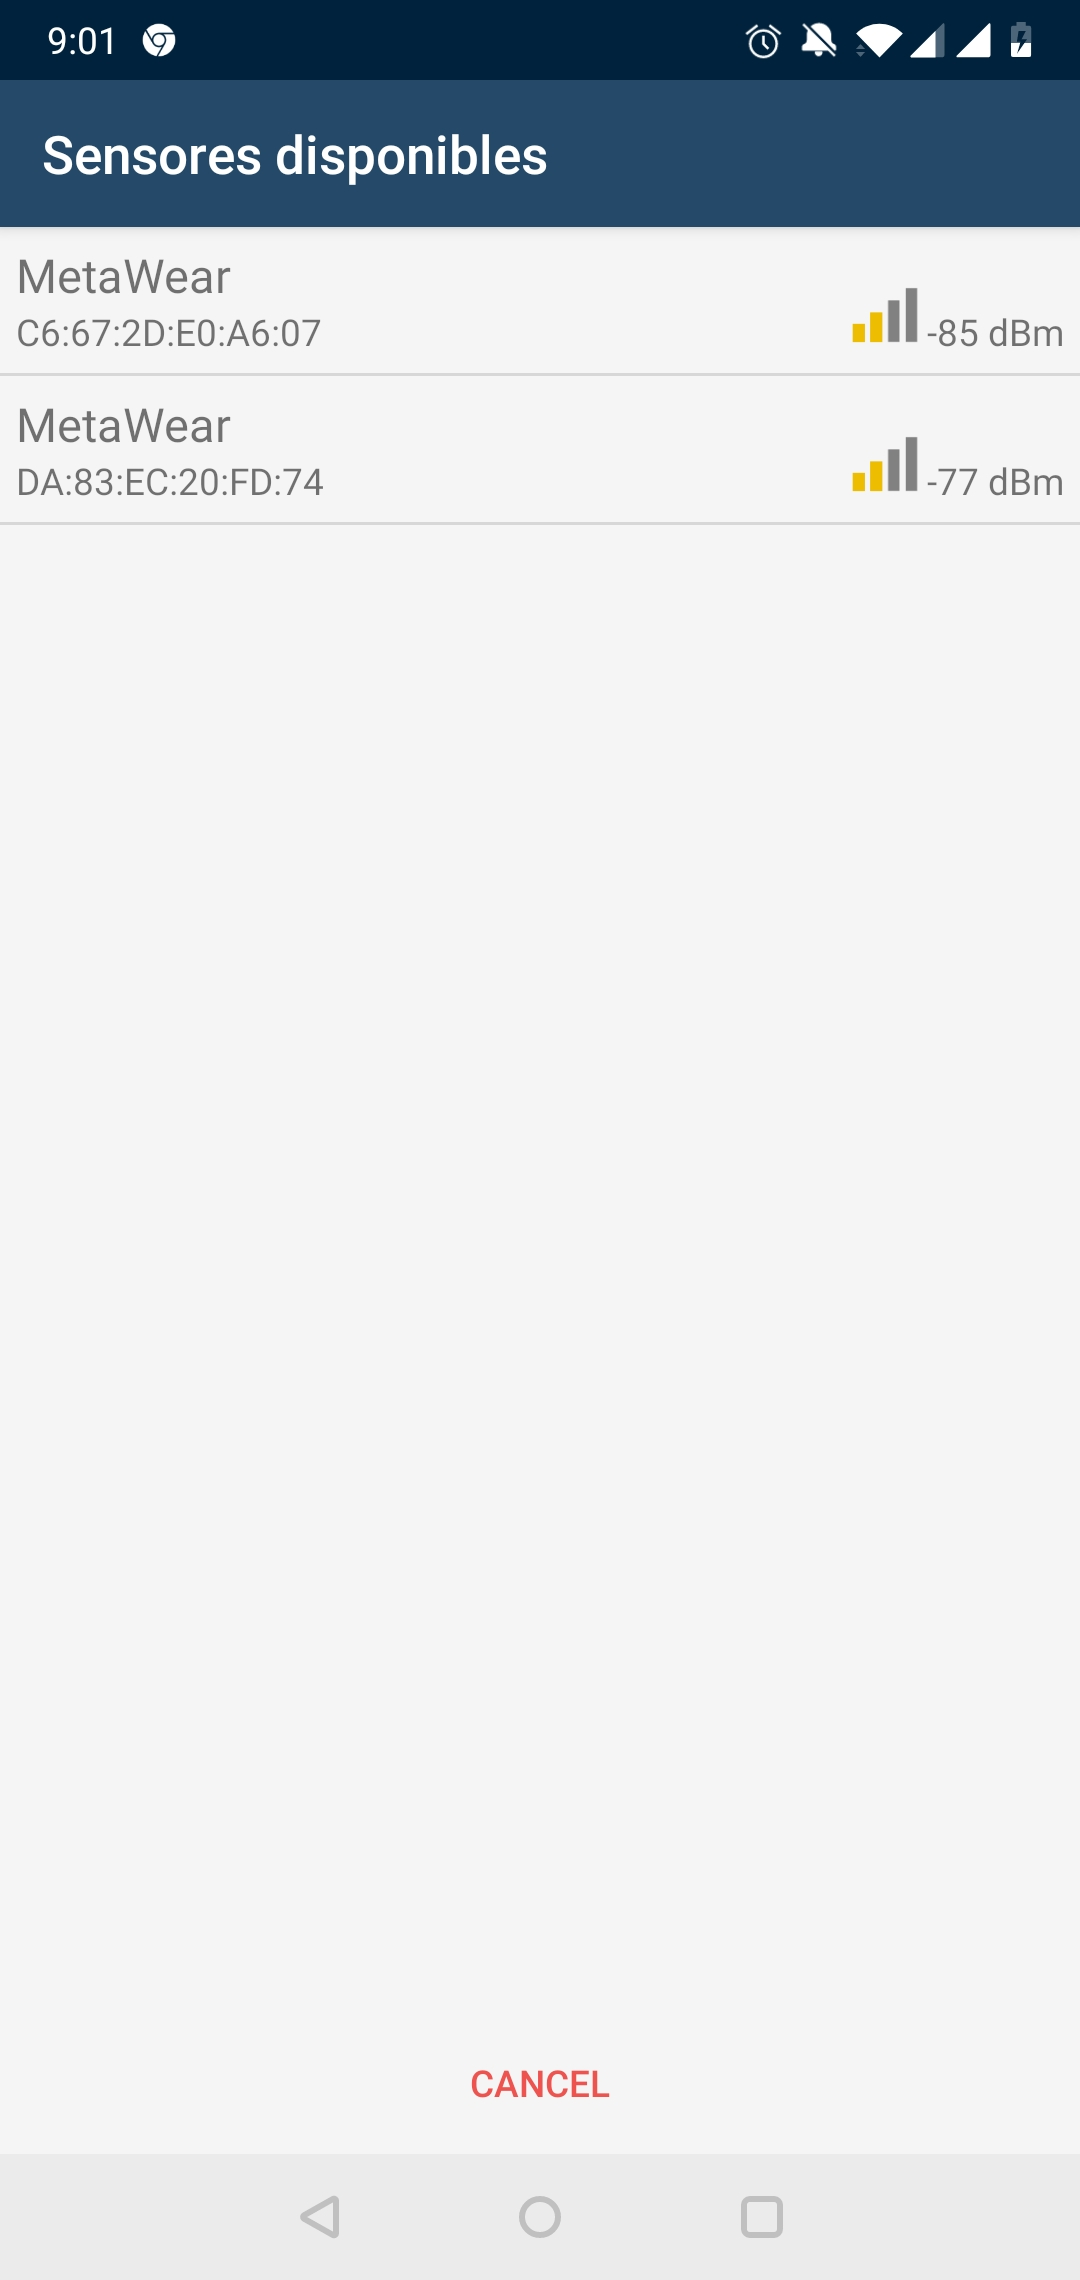
\includegraphics[height=8cm]{TESIS/imagenes/chap05/activity-searching-imus.JPG}
         \caption{Escaneo de dispositivos IMU. Previa activación del módulo bluetooth, expone un listado de IMU en la cercanía. Para cada uno muestra su dirección MAC, el tipo de IMU y la intensidad de la señal.}
     \end{subfigure}
     ~
     \begin{subfigure}[t]{0.4\textwidth}
         \centering
         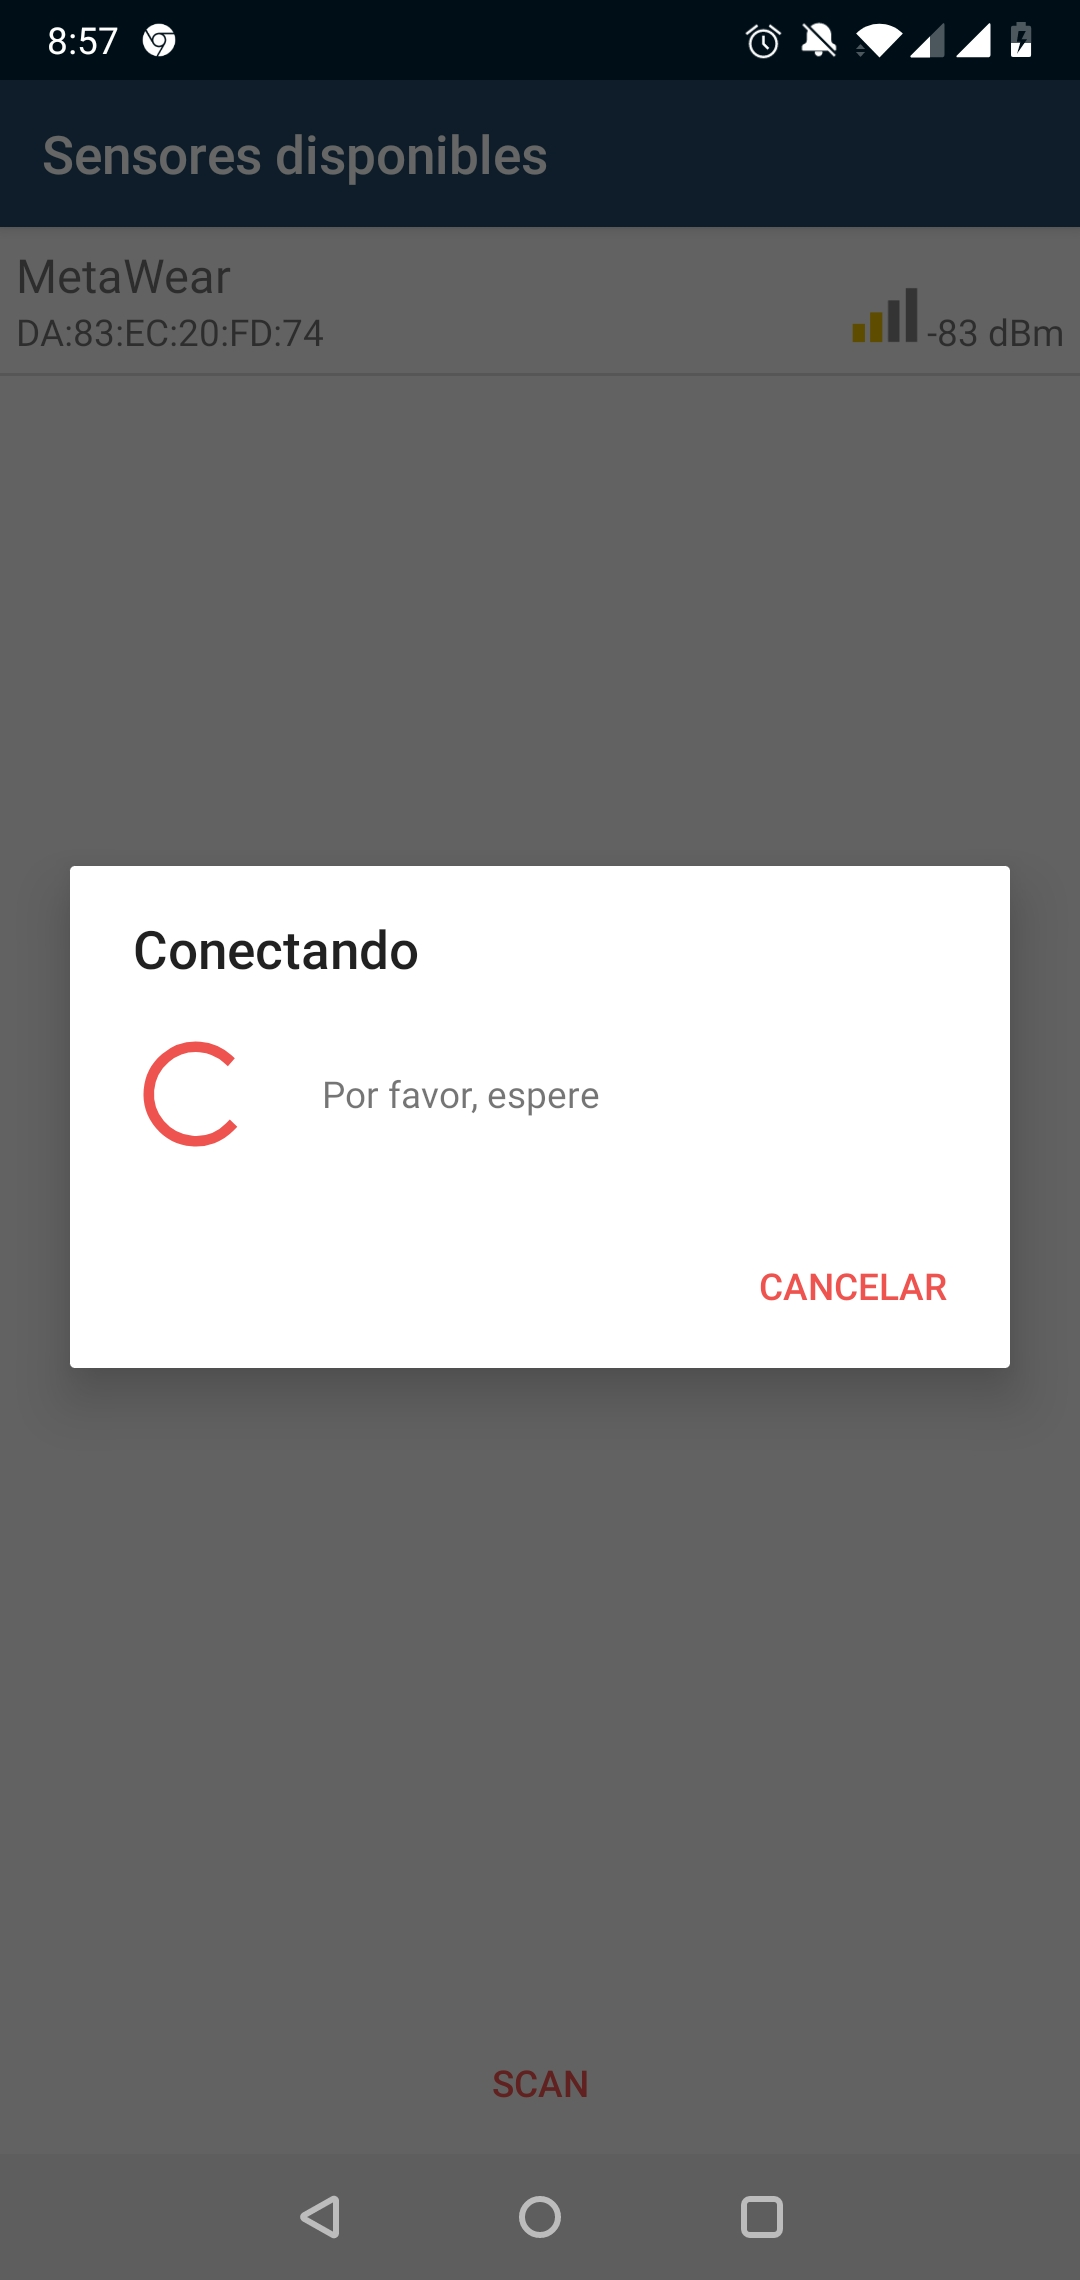
\includegraphics[height=8cm]{TESIS/imagenes/chap05/activity-connecting.JPG}
         \caption{Conexión en curso a un dispositivo IMU. Finalizada el proceso, el IMU es conectado exitosamente a PARKIBIP.}
     \end{subfigure}
     \caption{Proceso de escaneo previa a conexión de un IMU. Mediante el protocolo Bluetooth.}
     \label{fig:activity-scanning}
 \end{figure}

A continuación, se listan los módulos y algunas de las funciones principales que se emplearon en PARKIBIP:

\begin{enumerate}
    \item Bluetooth LE Connection: Gestión de la conexión entre aplicación Android y dispositivos IMU. 
    \begin{itemize}
        \item connectAsync: Establecimiento de conexión a un dispositivo.
        \item disconnectAsync: Remover la conexión a un dispositivo.
        \item UnexpectedDisconnect: Administración de eventos de desconexión inesperados.
        \item readDeviceInformationAsync: Obtener nivel de batería e información general del dispositivo.
        \item tearDown: Remueve los recursos asignados por el firmware del dispositivo.
    \end{itemize}
    \item \textit{DataProducer}: Componentes que recuperan datos, ya sean de sensores o de funciones del firmware.
    \begin{itemize}
        \item \textit{AsyncDataProducer}: Los productores de datos asincrónicos, cuando están activos, miden constantemente los datos en \gls{background} y los envían cuando hay nuevos datos disponibles.
        \item start: Inicia un productor de datos previamente configurado (e.g. sensor acelerómetro).
        \item stop: Remueve un productor de datos sin remover la conexión al hardware.
    \end{itemize}
    \item \textit{DataRoute}: Las rutas de datos proporcionan una forma simple y compacta para el acceso a las funciones avanzadas de \textit{MetaWear}, como el registro \textit{Log}, el procesamiento de datos y el manejo de eventos a bordo.
    \begin{itemize}
        \item addRouteAsync: creación de rutas de eventos, que definen cómo fluyen los datos desde un productor a diferentes puntos finales (a través de un \textit{RouteComponent}).
        \item Data: Los datos creados por los productores de datos están representados por la interfaz ``Datos'', que encapsula atributos de clave-valor, como la hora en que fueron creados los datos (timestamp) y el valor de la muestra de datos.
        \item stream: Permite el procesamiento del flujo de datos y como serán transformados los mismos. Establece un suscriptor al evento del productor de datos.
        \item log: Habilita a grabar datos en la memoria flash incorporada y recuperarlos en un momento posterior.
        \item state: Permite recuperar el vector de estados del dispositivo.
        \item buffer: Los almacenes son unidades que graban la entrada más reciente en su estado interno, y posteriormente permiten acceder mediante el método de estado (\textit{state}) perteneciente al módulo procesador de datos.
    \end{itemize}
    \item Function Module: Existen tantos módulos como sensores. Se listan funcionalidades genéricas a los módulos (Acelerómetro, giroscopio, magnetómetro, barómetro, luz ambiental, entre otros).
    \begin{itemize}
        \item start: Establece el uso de un módulo especifico.
        \item stop: Remueve el uso de un módulo especifico.
        \item configure: Configuraciones particulares a cada módulo.
        \item odr: Tasa de datos de salida.
        \item range: Rango de datos.
    \end{itemize}
\end{enumerate}

Es importante notar que, algunos de los nombres de los métodos disponibles finalizan con la palabra ``Async'', y significa que \underline{toda comunicación es asincrónica con el dispositivo}. Esto es un requisito a nivel del sistema operativo y es una característica esencial del sistema PARKIBIP, ya que el acceso a los datos del dispositivo no puede ser bloqueante. 

De esta manera, \underline{PARKIBIP es un sistema multihilo} (multithreading en inglés), teniendo la capacidad de ejecutar eficientemente múltiples hilos de ejecución y paralelizar diversas tareas en background, como por ejemplo los mensajes hacia o desde un dispositivo. Asimismo, esta tarea se complejiza aún mas, al escalar en número los dispositivos inerciales que puede gestionar el sistema. Entonces, se implementaron diversos hilos, para lograr:

\begin{itemize}
    \item Gestionar múltiples conexiones a dispositivos inerciales.
    \item Interactuar con los dispositivos mediante el envío y recepción de mensajes apropiados.
\end{itemize}

Se resalta la necesidad de diseñar e implementar diferentes estrategias para el control de concurrencia sobre recursos compartidos de los diversos Threads en simultanea ejecución.

\section{Administración de las conexiones}

Como se resaltó en la sección anterior \nameref{section:app-imu}, las conexiones entre la aplicación Android y un dispositivo Bluetooth se representan en una aplicación Android mediante la clase perteneciente al SDK de Android llamada \textit{BluetoothDevice}. Esta clase representa un dispositivo remoto conectado por Bluetooth, permitiendo a la aplicación comunicarse con el dispositivo, operar sobre él y requerirle datos como el nombre, dirección, clase, estado, batería, etc. 

Esta clase es realmente un fino \gls{wrapper} delgado para una dirección de hardware Bluetooth. Los objetos de esta clase son inmutables. Las operaciones en esta clase se realizan en la dirección de hardware Bluetooth remota, utilizando la clase \textit{BluetoothAdapter}. 

Para obtener un dispositivo Bluetooth, se utiliza la clase \textit{BluetoothAdapter}, con el método \textit{getRemoteDevice(String)}, la cual crea una instancia de \textit{BluetoothDevice} que representa un dispositivo de una dirección MAC conocida (que se puede obtener a través del descubrimiento de dispositivos también utilizando \textit{BluetoothAdapter}). Este descubrimiento se realiza en una pantalla dedicada dentro de la aplicación (en android representada con la clase \textit{Activity}), la cual llamamos \textit{ScannerActivity}. 

En la pantalla inicial de la aplicación, llamada \textit{MainActivity}, se le muestran al usuario botones para conectar cada uno de los dispositivos necesarios para el funcionamiento de PARKIBIP, uno para el pie izquierdo y otro para el pie derecho -ver Fig. \ref{fig:activity-conection-imu}-. 

\begin{figure}[!h]
     \centering
     \begin{subfigure}[t]{0.4\textwidth}
         \centering
         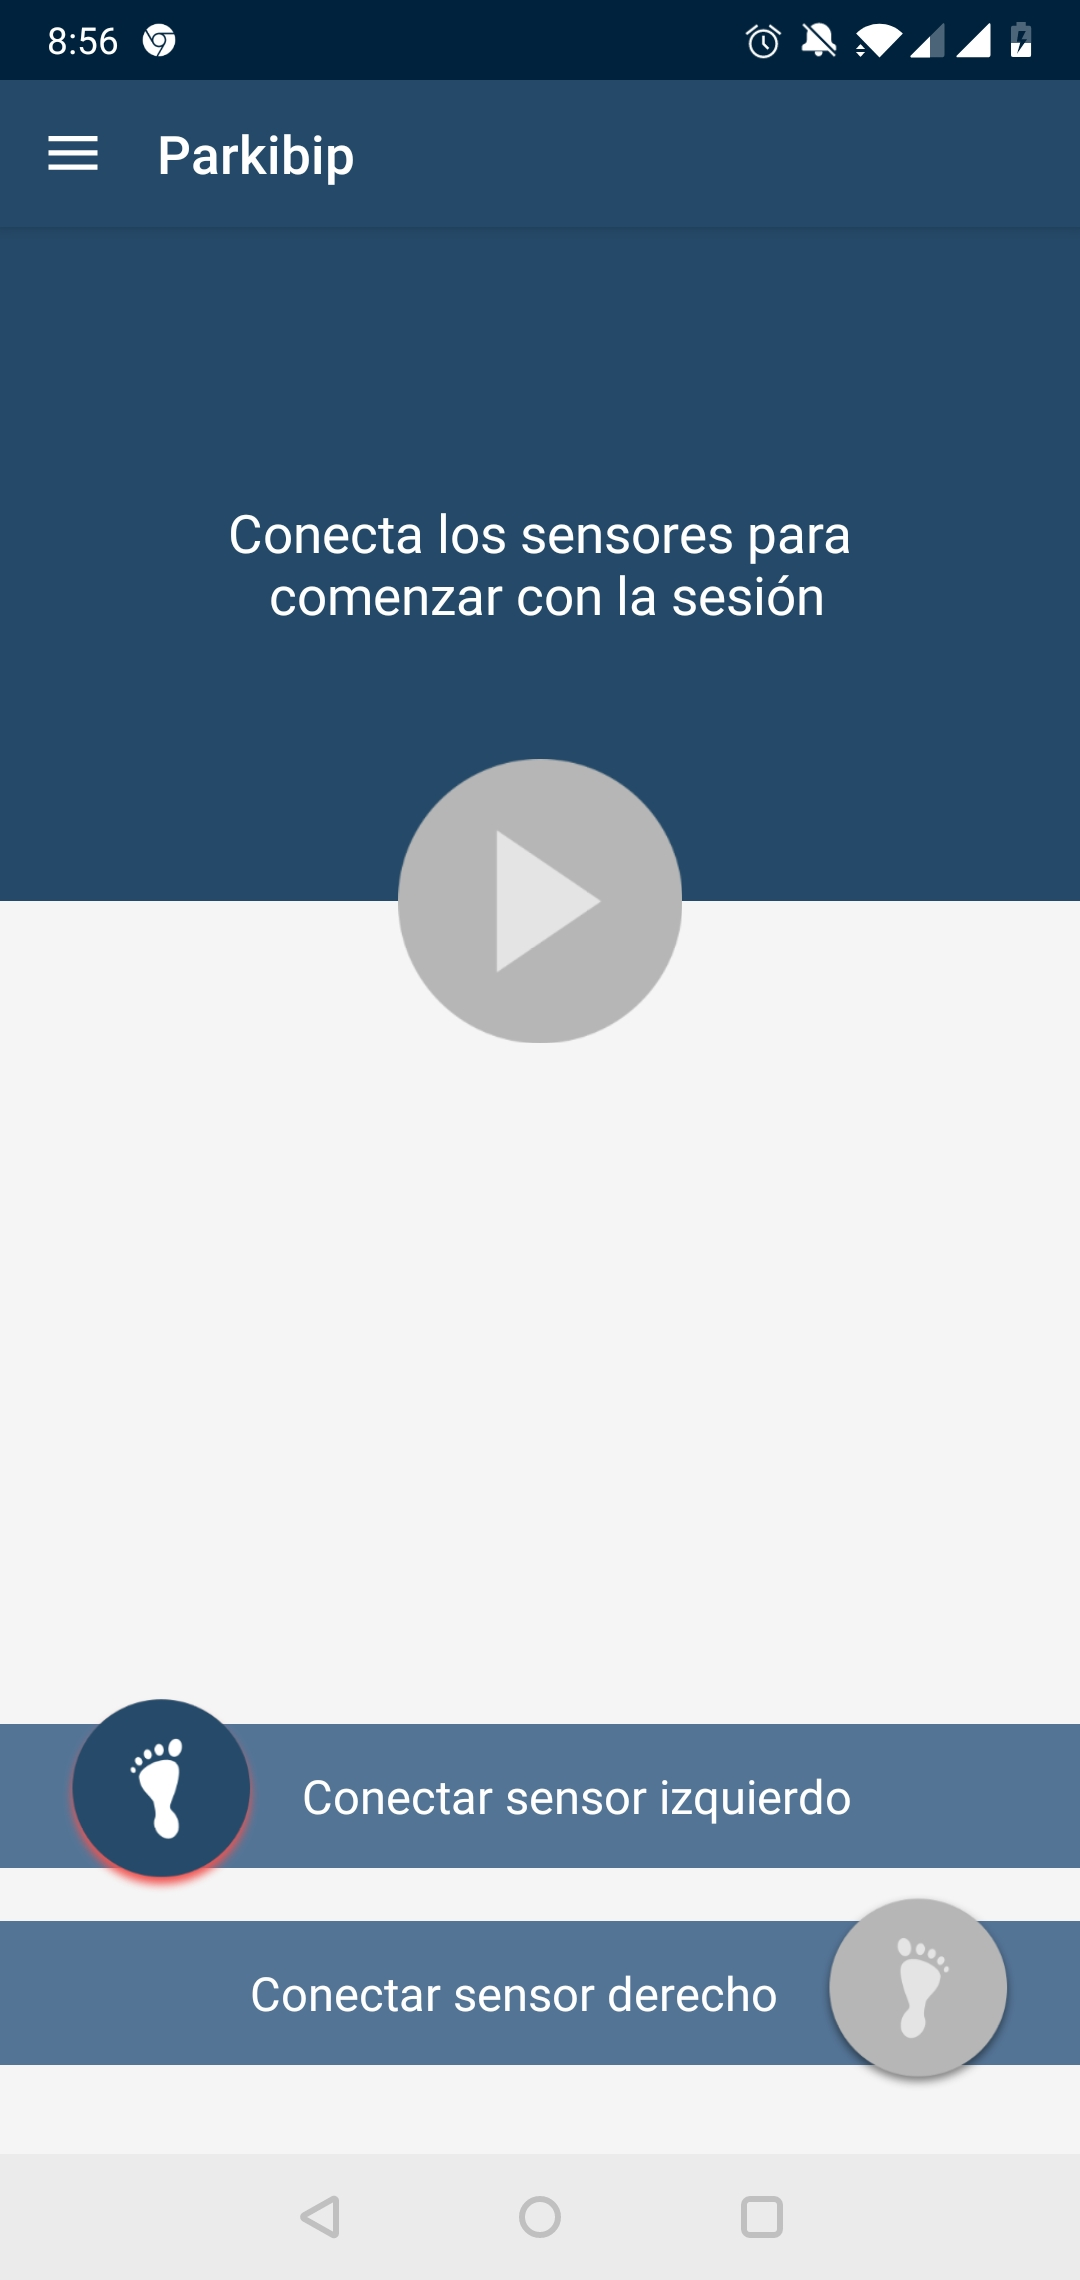
\includegraphics[height=8cm]{TESIS/imagenes/chap05/activity-selected-imu.JPG}
         \caption{Conexión exitosa del IMU asociado al pie izquierdo -botón coloreado de azul-. PARKIBIP identifica al Pie/IMU con un color en la aplicación, en la imagen rojo. Es el mismo color que comienza a parpadear en el IMU mediante su luz LED.}
     \end{subfigure}
     ~
     \begin{subfigure}[t]{0.4\textwidth}
         \centering
         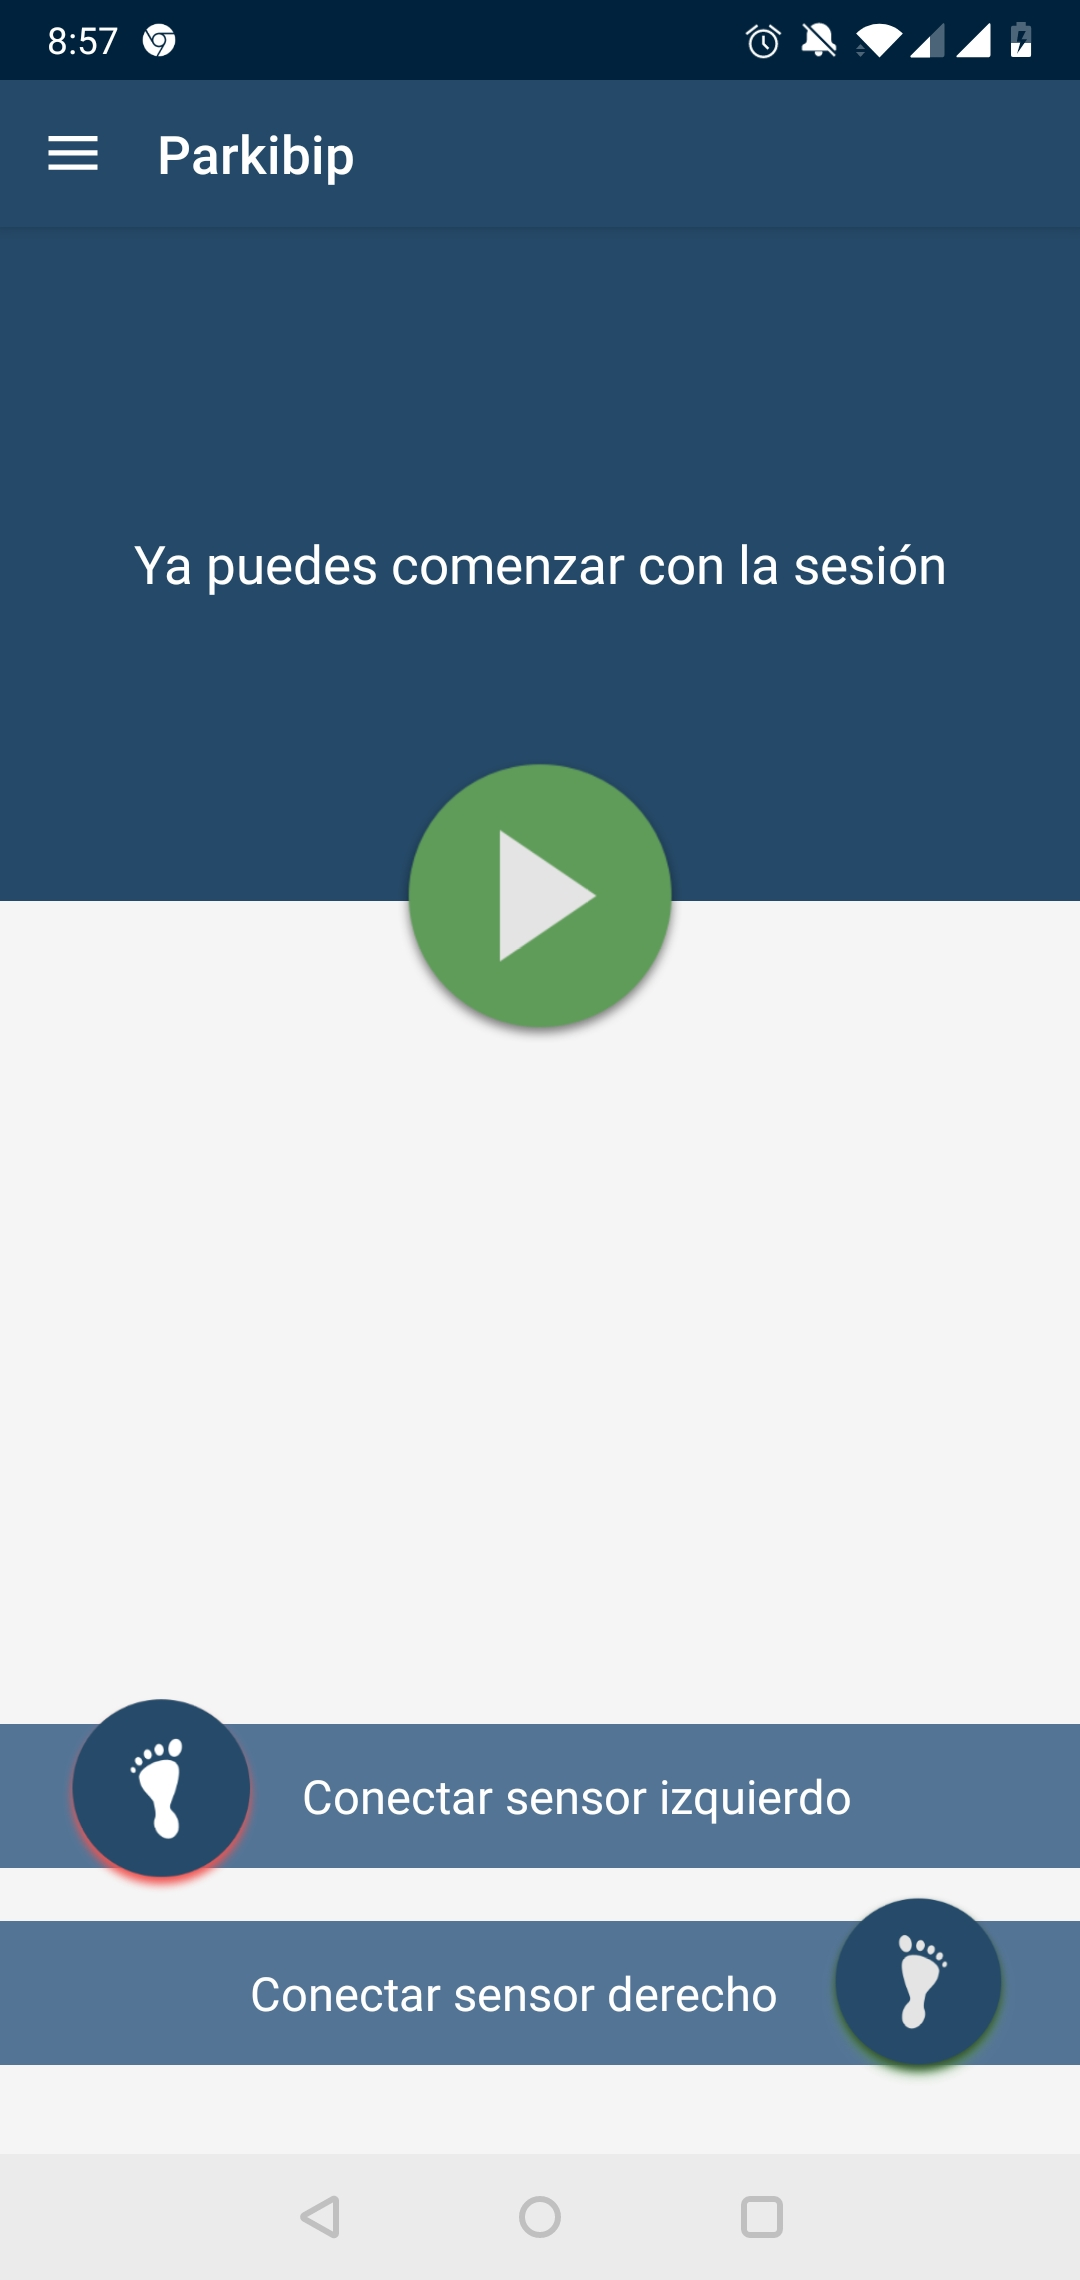
\includegraphics[height=8cm]{TESIS/imagenes/chap05/activity-ready-for-use.JPG}
         \caption{Conexiones a los IMU exitosa. Ambos botones se encuentra en azul, las luces LED del IMU sincronizadas a los colores de los contornos de los botones, y el botón central es puesto en verde. PARKIBIP se encuentra listo para comenzar una sesión de rehabilitación.}
     \end{subfigure}
     \caption{Conexiones a los dispositivos IMU mediante el protocolo Bluetooth.}
     \label{fig:activity-conection-imu}
 \end{figure}

Al seleccionar uno de estos botones se le muestra al usuario la pantalla de escaneo y selección de dispositivos IMU. Es importante destacar que el descubrimiento de dispositivos Bluetooth lo realizamos en esta pantalla filtrando la clase específica de dispositivos que requiere Parkibip, para que solo se listen dispositivos Bluetooth del tipo IMU y no algún otro dispositivo que pueda estar cerca del Smartphone. Una vez que la conexión se establece, la pantalla principal muestra un indicador de que el sensor para ese pie se encuentra conectado. Este indicador tiene un color específico que también se muestra a través de una luz Led en el sensor MMR (color rojo para el pie izquierdo y color verde para el pie derecho) que permite identificar qué sensor se debe colocar en cada pie. 

En el listado de cada uno de los dispositivos se muestra información pertinente sobre los dispositivos encontrados, como lo es su dirección MAC, el tipo de dispositivo, la intensidad de la señal (importante para el buen funcionamiento de la aplicación), entre otras cosas. 

Cuando el usuario selecciona un dispositivo, se realiza la conexión con el dispositivo y se obtiene una instancia de la clase \textit{BluetoothDevice} que utilizaremos para obtener los datos del dispositivo mientras el usuario realice la actividad. Resulta importante entonces proveer un mecanismo para administrar estas conexiones, mantener las instancias, identificarlas, liberarlas cuando sea necesario y que se realice su re-conexión en caso de que sea interrumpida. Con todos estos objetivos diseñamos el sistema como se muestra en la figura Fig. \ref{FIG:connections-management} 

\begin{figure}[H]
    \hspace*{-3.5cm}%
    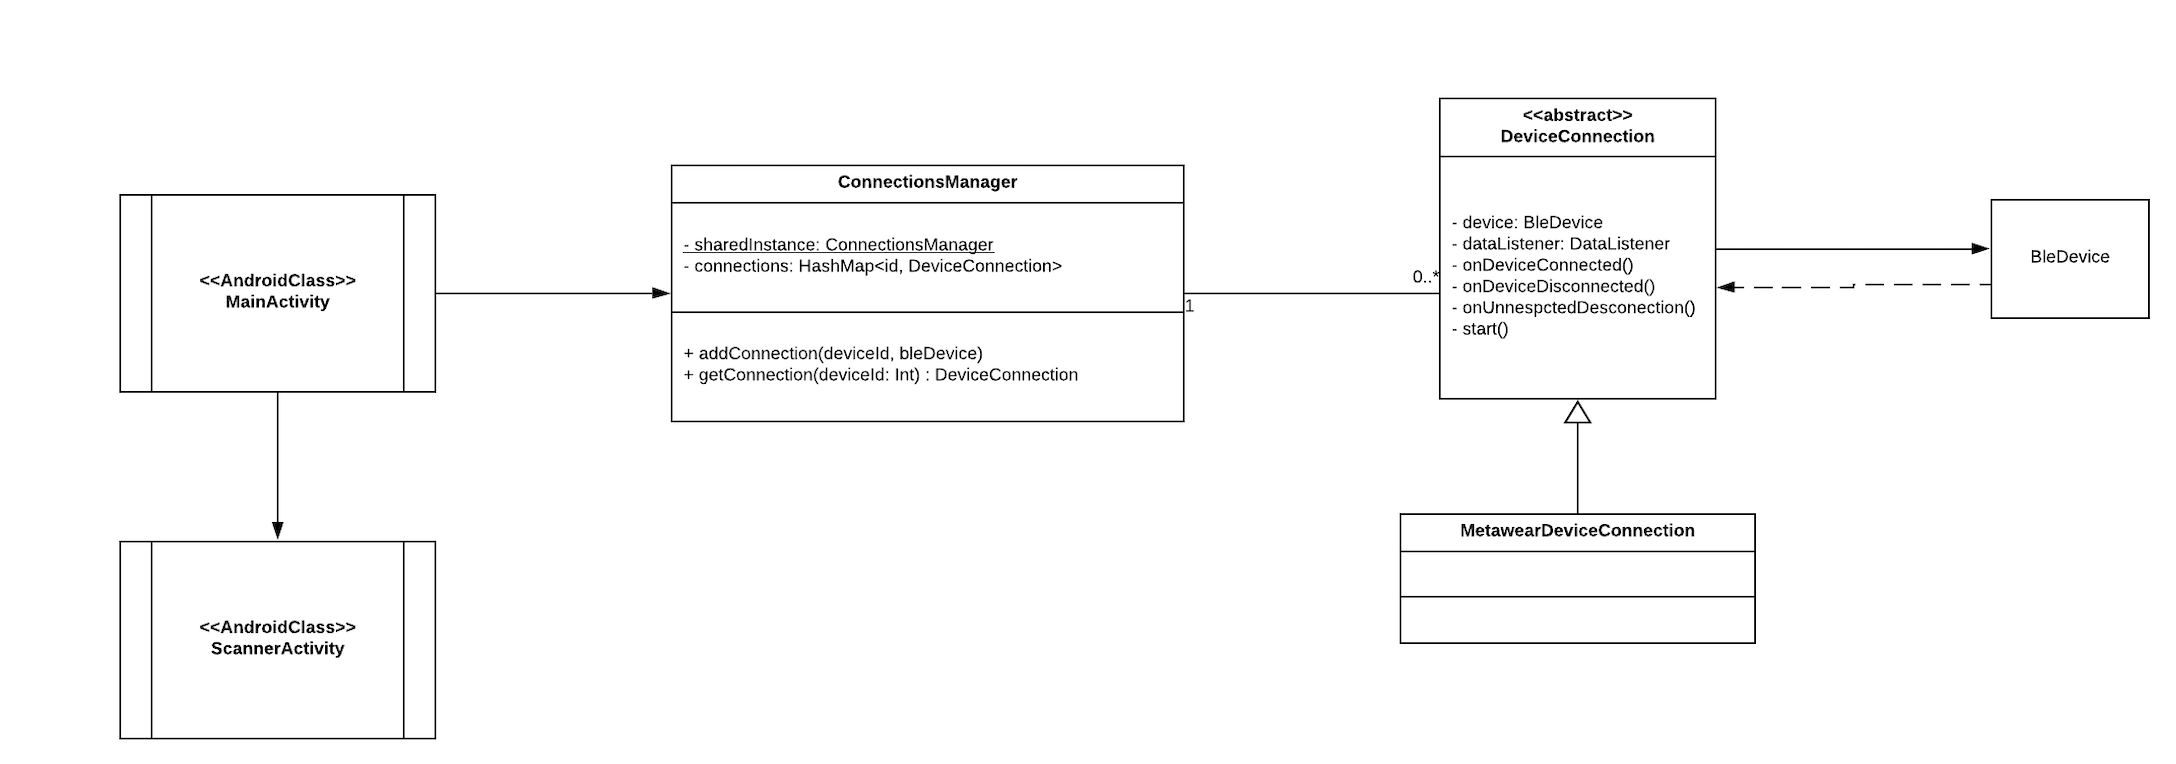
\includegraphics[clip,width=1.4 \columnwidth]{TESIS/imagenes/chap05/connections-management-design.png}
    \caption{Diagrama de clases del módulo de la aplicación Android donde se administran las conexiones Bluetooth con los dispositivos IMU}
    \label{FIG:connections-management}
\end{figure}

A continuación se describen las principales características del diseño, la interacción entre las clases y sus roles: 

\begin{itemize}
    \item La pantalla principal representada con la clase \textit{MainActivity} es encargada de crear y mostrar la pantalla de escaneo y selección de dispositivos (\textit{ScannerActivity}).
    \item En la pantalla \textit{ScannerActivity} el usuario selecciona el dispositivo y se crea la instancia de \textit{BluetoothDevice}.
    \item La pantalla \textit{MainActivity} recibe la instancia de \textit{BluetoothDevice} y se la provee a \textit{ConnectionsManager}. 
    \item \textit{ConnectionsManager} es un \textit{Singleton} con la única responsabilidad de administrar las conexiones existentes, guardadas en un Diccionario Clave-Valor (utilizando como clave un identificador de tipo \textit{String}).
    \item Cada conexión es mantenida por una instancia de la clase \textit{DeviceConnection}, una clase abstracta que representa el concepto de conexión con un dispositivo IMU. Estos objetos tienen la capacidad de mantener la conexión activa, solicitarle los datos al sensor, terminar el flujo, reconectarlo en caso de que la conexión sea interrumpida, entre otras cosas. 
    \item Para el dispositivo MetaMotionR se implementó una clase concreta de \textit{DeviceConnection} llamada \textit{MetaWearDeviceConnection}. La misma tiene una implementación concreta con las particularidades requeridas para comunicarse con este tipo de dispositivos, utilizando el SDK de MetaWear mencionado anteriormente.
\end{itemize}

El diagrama de comunicación de la Fig. \ref{FIG:addconnection-comm-diagram} detalla las distintas interacciones para el caso de uso ``Establecer conexión con dispositivo IMU''. 

\newpage

\begin{figure}[H]
    \hspace*{-3.0cm}%
    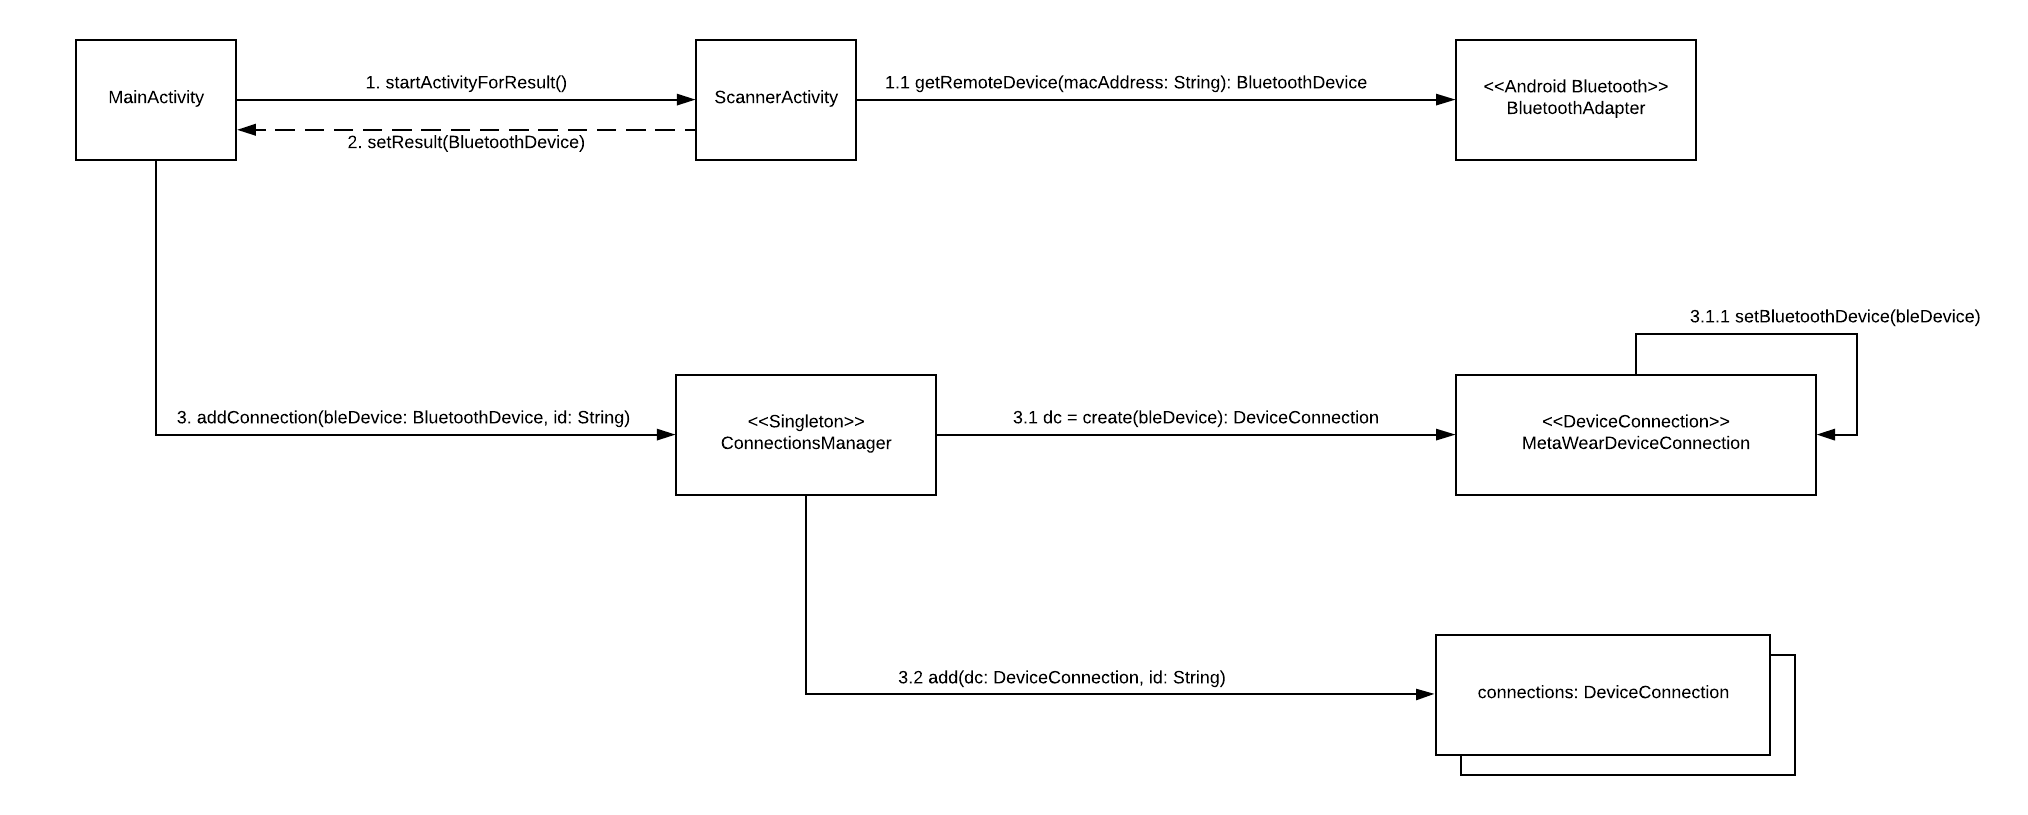
\includegraphics[clip,width=1.4 \columnwidth]{TESIS/imagenes/chap05/CreateConnection-CommDiagram.png}
    \caption{Diagrama de comunicación para el caso de uso ``Establecer conexión con dispositivo IMU''}
    \label{FIG:addconnection-comm-diagram}
\end{figure}

Este diseño nos provee de varias ventajas, a continuación nombramos algunas de éstas:

\begin{itemize}
    \item Las responsabilidades de cada clase están claras.
    \item Cada clase tiene una única responsabilidad.
    \item Agregar un nuevo tipo de dispositvo IMU -ya sea de otro proveedor de hardware, así como otro modelo de MbienLab- implicaría simplemente implementar una nueva clase concreta de la clase abstracta \textit{DeviceConnection}, lo que hace que el sistema sea escalable.
    \item Si en un futuro se quisiera utilizar más de dos dispositivos, este diseño funciona sin grandes cambios, ya que el manejador de conexiones \textit{ConnectionManager} puede mantener tantas conexiones como sea necesario 
    \item Este diseño soporta mantener conexiones con distintos tipos de dispositivos o de diferentes marcas de forma simultánea.
\end{itemize}
\newpage

% Como 1.Presentar Algoritmo de Fusión de datos
\section{Algoritmo de empaquetado de datos PARKIBIP}

Ya mencionado, la recopilación de datos de múltiples sensores de un dispositivo inercial, se realiza en diversos hilos de ejecución. Además, cada sensor opera con tasas de frecuencias eventualmente distintas -Hz-. Es fundamental combinar los datos recibidos -en hilos y frecuencias distintas- de manera adecuada, tal que los datos se mantengan consistentes.

Por lo tanto, se implementó un algoritmo de empaquetado de datos, con el objetivo de combinar valores de los sensores acelerómetro, giroscopio y magnetómetro en un único mensaje en cada instante de tiempo. Al fusionar varias fuentes de datos, es una restricción muestrear a la misma frecuencia, o al menos, múltiplos enteros de la frecuencia más rápida. 

El algoritmo desarrollado opera de la siguiente manera:
\begin{enumerate}
    \item Siempre se propagan los mensajes fusionados según la frecuencia mas alta
    \item El muestreo de fuentes de datos en las frecuencias más bajas repetirá el último valor recibido
    \item Se emplean dos colas de almacenamiento de mensajes, en modalidad de buffer FIFO (del inglés first-in, first-out), para las fuentes de datos cuyas frecuencias son mas bajas
\end{enumerate}

A continuación, se presenta el diagrama dado por la figura Fig. \ref{FIG: sensor-fuser}, el cual ejemplifica el procedimiento del fusión de datos.

\begin{figure}[H]
    \centering
    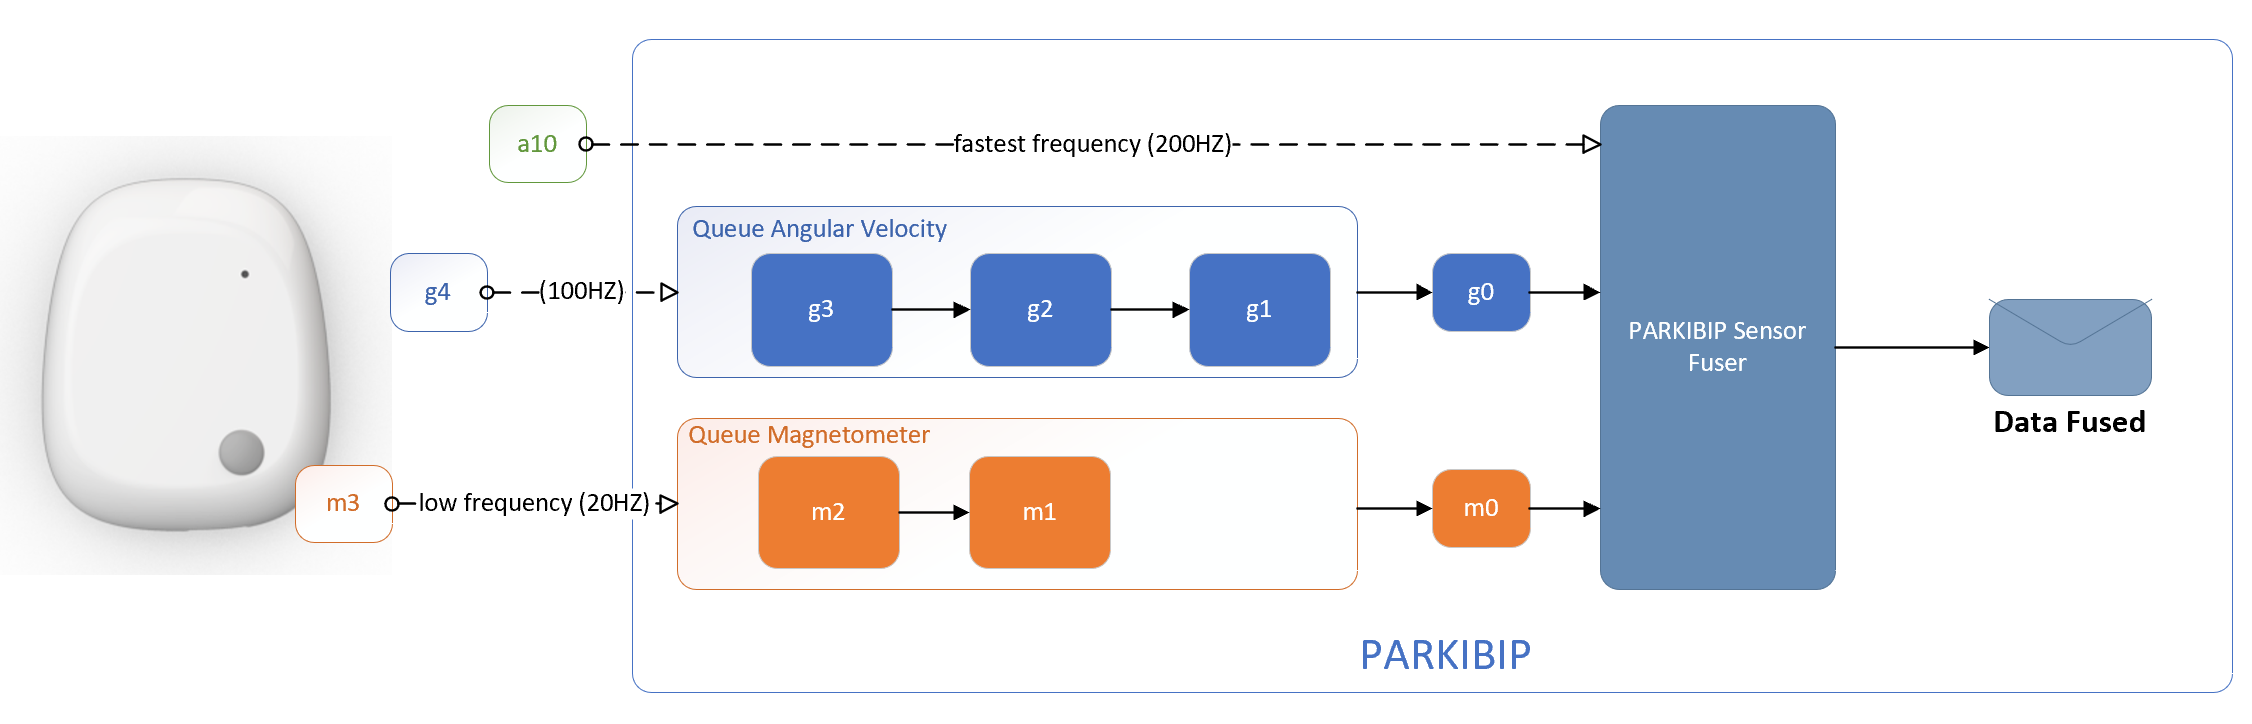
\includegraphics[clip,width=1.1 \columnwidth]{TESIS/imagenes/chap05/sensor-fuser.PNG}
    \caption{Algoritmo de empaquetado de datos PARKIBIP. Presenta un caso de uso de recopilación de datos de los sensores acelerómetro, giroscopio y magnetómetro en las frecuencias correspondientes 200HZ, 100HZ, 20HZ.}
    \label{FIG: sensor-fuser}
\end{figure}

% Como 2.0. API de Algoritmos (Quaternions, matrices, etc)
\section{Módulo de algoritmos numéricos y modelos de representación}\label{API-algoritmos} 

%Si o si hablar de cuaterion y propiedades, orientacion hace referencia
Puesto que PARKIBIP es un sistema físico-matemático complejo, el cual integra múltiples métodos numéricos y estadísticos; se optó por desarrollar un módulo destinado a la provisión de funciones independientes que aborden los problemas frecuentes. Este módulo, denominado ``API Algorithm'', tiene la responsabilidad de encapsular funciones reutilizables y particulares a la solución, para que luego sean accesibles desde cualquier método que las requiera.

En primer lugar, se introducen los principales modelos de representación que fueron empleados y gestionados dentro de la Interfaz de Programación de Aplicaciones (\gls{API}, Application Programming Interface) de algoritmos.
\noindent Conforme a representar la orientación del dispositivo en tiempo real, es necesario comprender los conceptos ángulos de euler (del inglés, Euler angles) y cuaternión (del inglés, Quaternion). Ambos modelos proporcionan una forma de representar la orientación de un cuerpo tridimensional mediante una combinación de tres rotaciones sobre diferentes ejes. Para el caso de los ángulos de euler, la secuencia de rotaciones utilizadas para representar una orientación dada es (i) yaw -rotación sobre el eje z un ángulo $\psi$-, (ii) pitch -rotación alrededor del eje Y un ángulo $\theta$-, (iii) roll -rotación alrededor del eje X un ángulo $\phi$-. Por otro lado, un quaternion es un vector de cuatro componentes, un elemento real y tres elementos complejos. Por ejemplo, $q^b_i = (a,bi,cj,dk)$  definido como el vector unitario que codifica la rotación desde el marco inercial hacia el marco del sensor. Luego, ambas representaciones pueden ser utilizadas para construir una matriz de rotación $R_{3X3}$ para realizar la rotación en una sola operación de multiplicación de matrices.

En vista de los modelos de representación introducidos y las necesidades operatorias del sistema, se implementaron las funciones necesarias para manipular y operar con éstos modelos de representación. En seguida, se listan algunas funciones desarrolladas en la API de algoritmos:

\begin{enumerate}
    \item Medición
    \begin{itemize}
        \item adjustMeasurementUnities(MeasurementModel measurementModel): Estandariza las unidades de las mediciones hacia los sistemas internacionales de unidades $m/s^2$ para aceleraciones y radianes para el caso de velocidades angulares.
        \item buildMeasurementWithData(Data data): Convierte una instancia genérica de la clase Data retornada por el IMU a su correspondiente modelo en PARKIBIP (MeasurementModel).
        \item buildMeasurement(Acceleration acceleration, AngularVelocity angularVelocity, MagneticField magneticField, Calendar timestamp): Crea una instancia lógica de MeasurementModel con el timestamp adecuado, a partir de los vectores tridimensionales acelerómetro, giroscopio y magnetómetro.
    \end{itemize}
    \item Filtro de Orientación
    \begin{itemize}
        \item updateOrientation(MeasurementModel measure, boolean hasMg): Función responsable de ejecutar el filtro de orientación implementado y retornar el nuevo quaternion. El parámetro \textit{hasMg}, indica la existencia de una observación del tipo magnetómetro.
    \end{itemize}
\item Aceleración  
\begin{itemize}
    \item romoveGravityForces: Método responsable de la extracción de la aceleración instantánea física del sensor.
    \item getUserAcceleration(MeasurementModel measure): Función encargada de obtener la aceleración del usuario en el marco inercial, resultado de la transformación de marcos y remoción de fuerzas gravitatorias.
    \item linearAccelerationMethod(MeasurementModel measure): Algoritmo responsable de computar la aceleración lineal instantánea del sensor.
\end{itemize}
\item Giroscopio
\begin{itemize}
     \item deg2rad(float degrees): Convierte el valor de grados a radianes para los datos del giroscopio.
    \item rad2Deg(float radians): Convierte el valor de radianes a grados para los datos del giroscopio.
\end{itemize}
\item Orientación
\begin{itemize}
    \item quaternProd(QuaternionModel q1, QuaternionModel q2): Función responsable de calcular el producto de dos cuaterniones.
    \item vectorFromRotationMatrix(RotationMatrix r, MeasurementModel measure): Dada una medición en el marco del sensor, aplica la Rotación por parámetro, para trasladar el vector a un marco de referencia inercial.
    \item vectorFromQuaternionProd(QuaternionModel q, MeasurementModel measure): Dada una medición en el marco del sensor, aplica la rotación dada por la orientacion en formato quaternion, para trasladar el vector a un marco de referencia inercial.
    \item convertToRotationMatrix(QuaternionModel q): Convierte un quaternion a su correspondiente matriz de rotación.
    \item convertToEulerAngles(QuaternionModel q): Convierte un quaternion a sus correspondientes ángulos de euler.
    \item getQuaternion(): Retorna el ultimo quaternion calculado por el filtro de orientación.
    \item dcm2q(double[][] rot): Convierte una matriz de cosenos de dirección al respectivo quaternion.
    \item rt2b(RealVector attitudeVector): Calcula y retorna la matriz de rotación desde un marco inercial al marco del sensor, a partir de los ángulos de euler.
\end{itemize}
\item Calibración
\begin{itemize}
  \item calibrateQuaternion(MeasurementModel measurementModel): Método iterativo responsable de calibrar adecuadamente la orientacion inicial del dispositivo IMU.
    \item stopCalibrateQuaternion(): Interrumpe un proceso de calibración retornando el ultimo quaternion computado.
    \item hasToStopCalibrate():  Chequea si es necesario interrumpir un procedimiento de calibración de orientación previamente iniciado. En caso de requerirse, retorna verdadero.
    \item hasToCalibrate(): Chequea si es necesario efectuar una calibración de orientación. En caso de requerirse, retorna verdadero.
\end{itemize}
\item Timestamp
\begin{itemize}
  \item getDiffSeconds(Calendar timestampOld, Calendar timestampNew): Obtiene la diferencia entre dos marcas de tiempos del tipo Calendar. 
\end{itemize}
\end{enumerate}

%TODO: agregar referencia a Apache 
Finalmente, para llevar adelante las distintas representaciones de matrices y vectores, asi como el algebra subyacente, se incluyó la librería de la compañía Apache, referida como ``Apache Commons Math'' \cite{apacheCommons}. La misma proporciona diversas funciones ligeras en el lenguaje de programación JAVA, representaciones numéricas escalables (e.g. naturales, reales, precisión simple y doble); por ende, facilita su utilización y reutilización independientemente de la complejidad requerida. 

En este sentido, es importante notar la complejidad de PARKIBIP relativa a la precisión numérica requerida, es decir, operaciones matriciales complejas y con valores numéricos que descienden aproximadamente a $10^{-22}$.

% Como 2.1.Marcos de referencia 
\section{Sistemas de coordenadas de referencias } \label{section:coordenadas}

Para lograr analizar la marcha de personas, así como también comprender el significado de las mediciones, es necesario identificar los sistemas de coordenadas que intervienen en el proceso.

%Sistema de coordendas
Puesto que los dispositivos inerciales IMU son colocados en los tobillos de los sujetos, existen tres sistemas de coordenadas: el marco de referencia Pie -que describe la rotación del pie-, el marco Sensor -que describe el movimiento del dispositivo inercial- y el marco fijo Inercial o Terrestre -ver figura Fig. \ref{fig:sensor-frame}-. Dado que el IMU se encuentra fijado al pie del sujeto mediante bandas elásticas de velcro, se asume que el dispositivo no se desliza ni se mueve durante la marcha. Por lo tanto, se considera que el sistema de coordenadas del pie es igual al sistema de coordenadas del Sensor.

%Procedimiento rotación y acele remover gravedad
El procedimiento consiste en recopilar las observaciones recibidas desde los distintos sensores, estimar la orientación de cada dispositivo en tiempo real; y luego transferir -mediante cuaterniones o rotaciones- el marco del sensor al marco inercial de la Tierra. Como consecuencia, es posible operar y realizar un análisis de la marcha desde un marco de referencia fijo, estandarizado y conocido.

\newpage

\begin{figure}[H]
\centering
\begin{subfigure}[b]{0.5\textwidth}
  \centering
  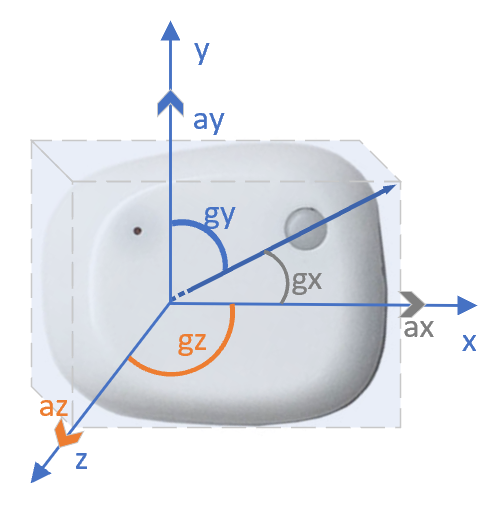
\includegraphics[width=\textwidth]{TESIS/imagenes/chap05/sensor-frame.PNG}
  \caption{Marco del Sensor IMU (S) de los ejes del acelerómetro y giroscopio, según especificación.}
  \label{fig:sfig1}
\end{subfigure}%
\begin{subfigure}[b]{0.5\textwidth}
  \centering
  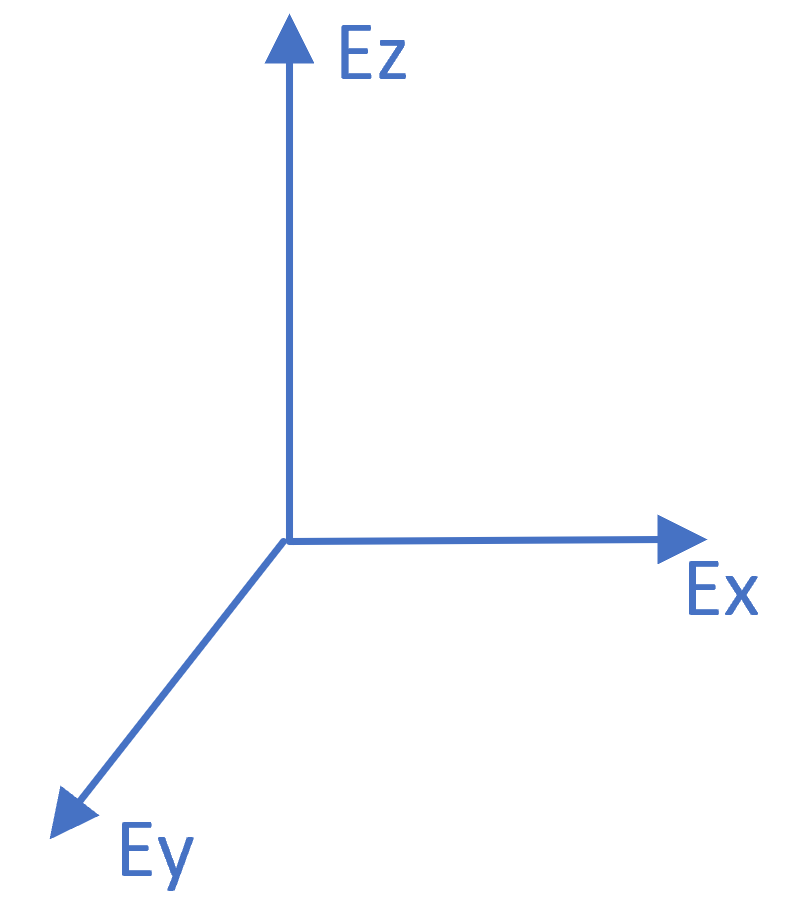
\includegraphics[width=\textwidth]{TESIS/imagenes/chap05/frame-earth.PNG}
  \caption{ Marco inercial Tierra (E). }
  \label{fig:sfig2}
\end{subfigure}
\begin{subfigure}[b]{0.5\textwidth}
  \centering
  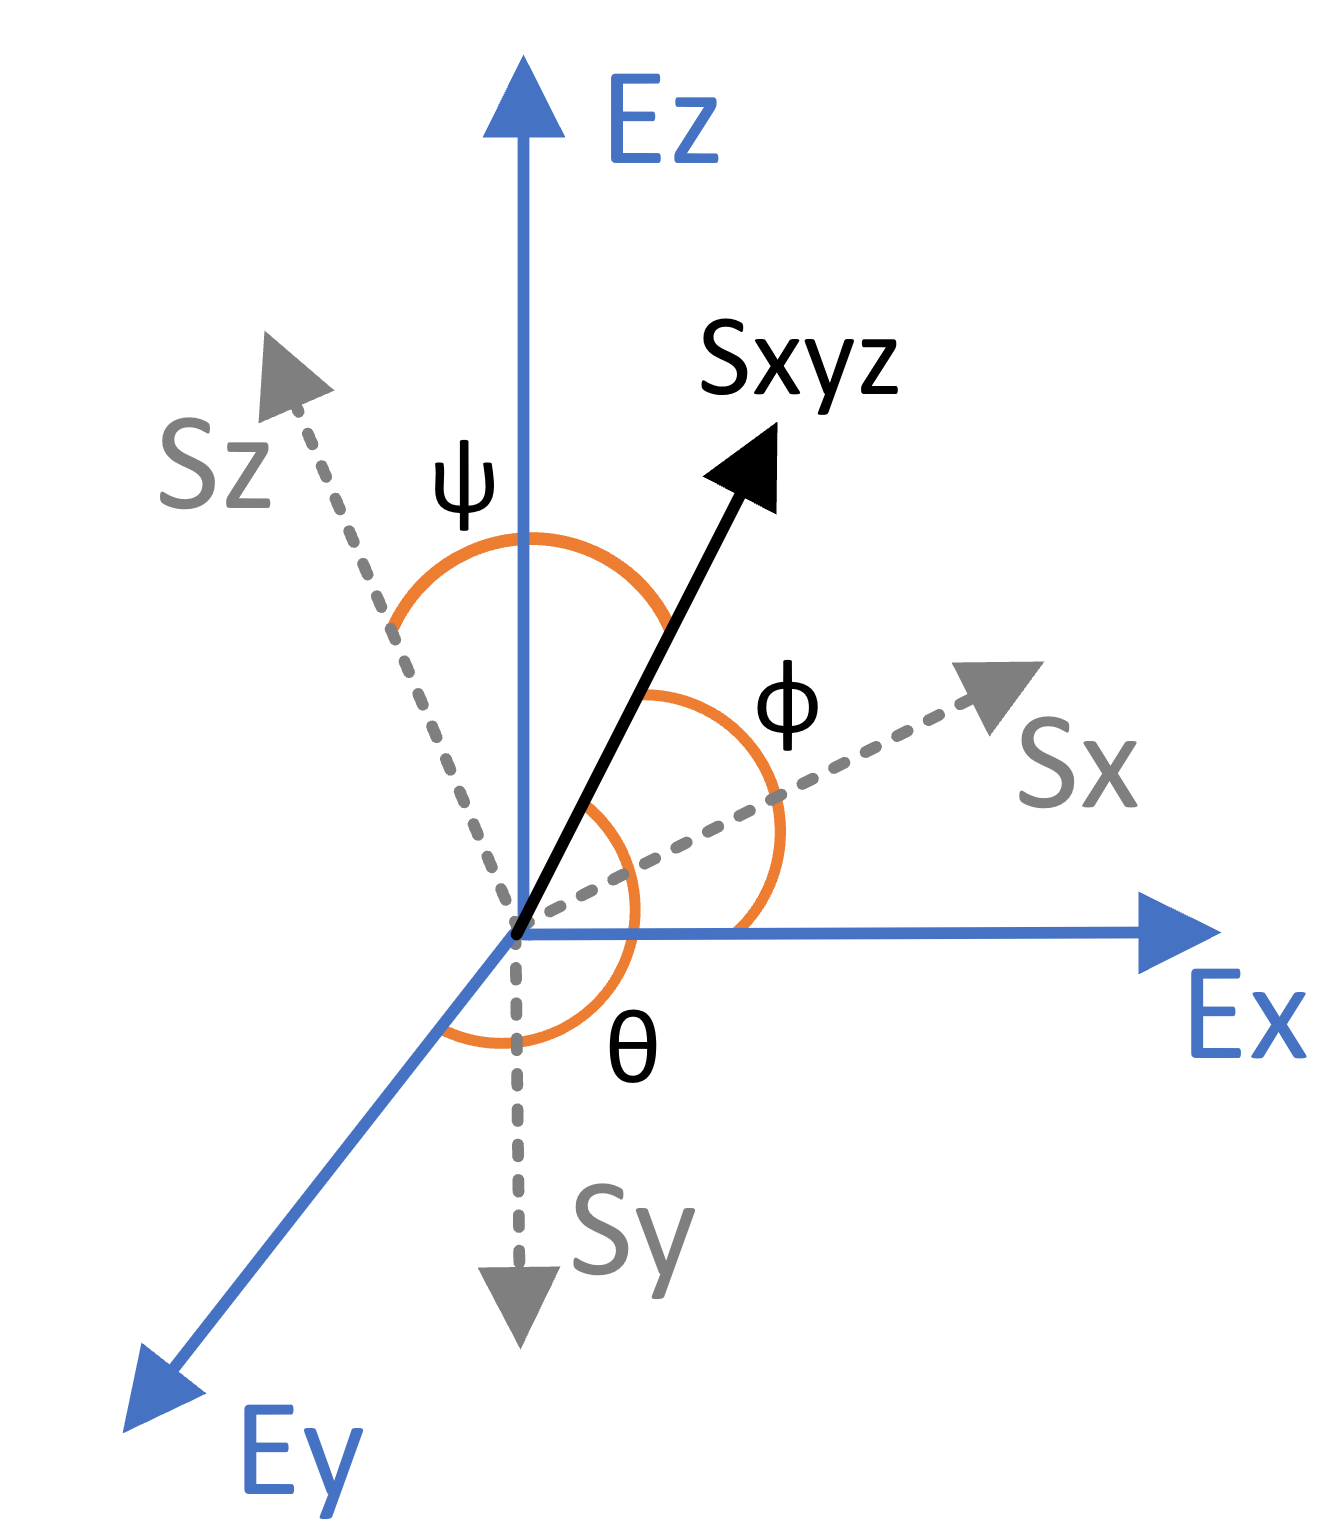
\includegraphics[width=\textwidth]{TESIS/imagenes/chap05/frame-translation.PNG}
  \caption{La orientación del marco E se logra mediante una rotación, desde la alineación con el marco S, de un ángulo de ($\phi,\theta ,\psi$) = (roll,yaw,pitch) alrededor del eje $S_{xyz}$.}
  \label{fig:sfig2}
\end{subfigure}
\caption{Tres ejes de coordenadas dimensionales del IMU. Sistemas de coordenadas de referencia del Sensor ($S_XS_YS_Z$) e Inercial ($E_XE_YE_Z$), traslación del vector en S hacia E, mediante rotación de ángulos. }
\label{fig:sensor-frame}
\end{figure}

% Como 2.1.Presentar Madwick
\section{Algoritmo Filtro de Orientación} \label{impl:orientation-filter}

Para estimar la orientación de los dispositivos respecto a un sistema de referencia inercial, se decide aplicar la técnica de \textit{gradiente descendiente optimizado y derivado analíticamente} sugerida por S. Madgwick -toma de decisión en \nameref{section:filter_orientation}-, descripta en la figura FIG. \ref{FIG: madgwick} tomada de \cite{Madgwick}. El método, presenta grandes ventajas, logrando excelentes resultados en la estimación y siendo computacionalmente eficiente.

\begin{figure}[H]
    \centering
    \resizebox{\textwidth}{!}{
    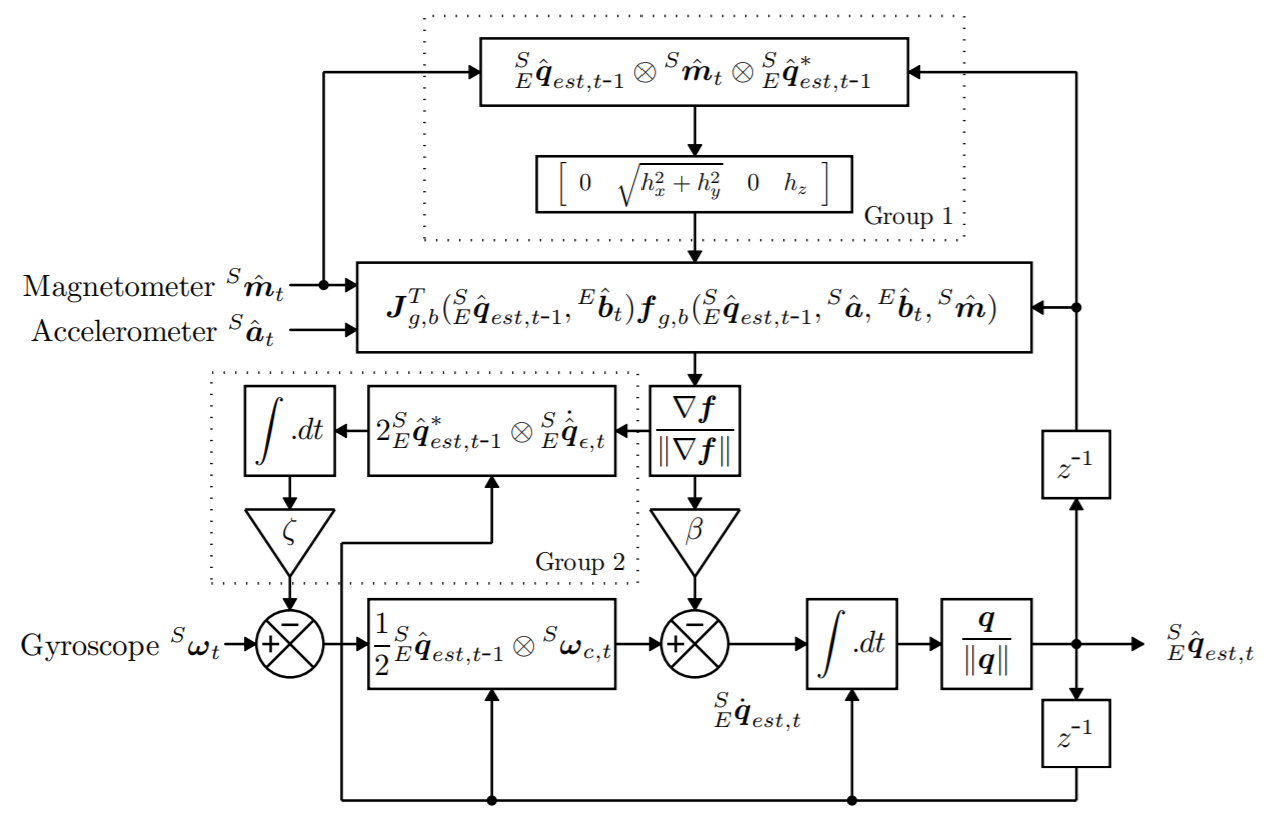
\includegraphics{TESIS/imagenes/img/madgwick.png}}
    \caption{Filtro de orientación con distorsión magnética. Extraído de S. Madgwick \cite{Madgwick}.}
    \label{FIG:madgwick}
\end{figure}

En primer lugar, se realizó un relevamiento respecto a implementaciones de código abierto del algoritmo en el mismo lenguaje de desarrollo que PARKIBIP -de forma que se pueda reutilizar directamente-. No obstante, no se encontró una implementación oficial o alternativa en el lenguaje JAVA, y  si se obtuvo un ejemplo en el lenguaje \textit{Matlab} que sirvió como guía en el desarrollo y pruebas funcionales de PARKIBIP.

Por lo tanto, fue implementado en Android -JAVA- el flujo descripto en la figura Fig. \ref{FIG:madgwick} combinando los datos sensados por el acelerómetro, giroscopio y magnetómetro del dispositivo IMU.

%Hablar de la representacion y el resultado de quaternion
Mencionado en las secciones \nameref{API-algoritmos} y \nameref{section:coordenadas}, existen varias formas de representar la información de orientación de un cuerpo, como por ejemplo los ángulos de Euler o los cuaterniones. Un cuaternión es un número complejo de cuatro dimensiones que se puede utilizar para representar la orientación de un cuerpo o un marco de coordenadas en un espacio tridimensional. Si bien son menos intuitivos que los ángulos de Euler y las matemáticas pueden ser un poco más complejas, presentan ciertas ventajas -entre ellas, no padece ``Gimbal lock'', que impide medir la orientación cuando el ángulo de inclinación se acerca a los +/- 90 grados-, y por lo tanto son empleados en la implementación de PARKIBIP.

Es crucial identificar adecuadamente los marcos de referencias y cómo los mismos son interpretados para obtener resultados esperados. Así, se utilizó un sistema de notación de superíndices y subíndices adoptado en \cite{1987Merat}, para denotar los marcos relativos de orientaciones y vectores. Un subíndice denota el marco que se está describiendo y un superíndice denota el marco al que se hace referencia. Por ejemplo, \textbf{$q_{B}^{A}$} describe la orientación del marco B relativo al marco A.

Como se puede apreciar en el modelo \ref{FIG:madgwick}, las observaciones acelerómetro, giroscopio y magnetómetro en el sistema de coordenadas del sensor, actúan como entrada al algoritmo numérico. A partir de dichos datos y el estado del cuaternión previo, se computa la orientación completa del sensor respecto al marco de referencia inercial Tierra. 

\begin{table}[H] 
\caption{Descripción, notación y tipo -entrada o salida- de los parámetros empleados por el algoritmo filtro de orientación.}
\centering
\begin{tabular}{ |c|c|c| } 
 \hline
 \textbf{Descripción} & \textbf{Parámetro} & \textbf{Notación} \\ \hline
 Magnetómetro en el marco del sensor  instante t & Entrada & $m_{t}^{s}$    \\ \hline
 Acelerómetro en el marco del sensor  instante t & Entrada & $a_{t}^{s}$  \\ \hline
 Giroscopio en el marco del sensor instante t & Entrada & $g_{t}^{s}$   \\ \hline
 Orientación de la Tierra relativa al sensor & Salida & $_{E}^{S}\hat{q}_{est,t}$  \\ 
 \hline
\end{tabular}
\end{table}

Finalmente, con la estimación de la orientación completa, es posible rotar un vector de un marco de referencia a otro, particularmente las observaciones tridimensionales sensadas por el IMU. Logrando de esta manera, estandarizar los concepto para un posterior análisis. Un posible procedimiento de rotación de un vector en el marco del Sensor a uno inercial -empleando propiedades particulares de cuaterniones, e.g. el cuaternión conjugado es el inverso de los marcos $q_{S}^{E} = (q_{E}^{S})^{-1}$- es:

\begin{align*}
    v_E&=q_{S}^{E}\cdot v_S \cdot q_{E}^{S}\\
    V_S&: \text{vector en el marco del Sensor}\\
    V_T&: \text{vector en el marco inercial}
\end{align*}

% Como 2.2 Presentar Algoritmo  Zero velocity. Como detecta las fases?

\section{Extracción de la aceleración física del sensor}

En general, las estimaciones de posición y velocidad basadas en acelerómetros de sensores de bajo costo son muy malas e inutilizables. Esto se debe a que la orientación del sensor debe conocerse con un alto grado de precisión para que las mediciones de gravedad se puedan distinguir de la aceleración física del sensor. Ya mencionado, pequeños errores en la estimación de la orientación producirán errores extremadamente altos en la aceleración medida, lo que se traduce en errores aún mayores en las estimaciones de velocidad y posición. Aunque en PARKIBIP el calculo de la posición y velocidad no dependerán únicamente del acelerómetro para mejorar su eficacia -también del giroscopio y magnetómetro-; es crucial eliminar la aceleración gravitatoria incluida en la aceleración sensada.

Entonces, para convertir la medición del acelerómetro en la aceleración física real del IMU -o aceleración del usuario-, es importante comprender exactamente lo que mide éste sensor. En este sentido, el acelerómetro mide tanto la aceleración física del sensor como la contribución de las fuerzas normales que evitan que el acelerómetro acelere hacia el centro de la Tierra. Para medir solamente las componentes de aceleración que son causadas por la aceleración física, las fuerzas normales debe ser removidas. Es decir:

\noindent Sea $am_{S}$ la aceleración del movimiento sensada en el marco del Sensor, $au_{E}$ es la aceleración real del dispositivo en el cuerpo -del usuario-, $g_{E}$ el vector de componentes gravitatorias en el marco inercial, y $R_E^S$ es la matriz de rotación desde el marco inercial a el marco del Sensor:

\[
    am_{S} = au_{S} - R_E^S \cdot \vec{g}, \quad \vec{g} =   \begin{pmatrix}
      0\\
      0\\ 
      g
\end{pmatrix} 
\]  
\noindent Conforme a eliminar las componentes gravitatorias de la medición de aceleración y obtener la aceleración del usuario, se deduce que:

\begin{equation*}
     au_{S} = am_{S} + R_E^S \cdot \vec{g} 
\end{equation*}

\noindent Obteniendo $au_{E}$, la aceleración del movimiento del usuario en el sistema de coordenadas inerciales:
\begin{equation*}
    au_{E} = R_S^E \cdot am_{S} + \vec{g}
\end{equation*}  
    
\noindent Cabe resaltar que, \underline{la matriz de rotación ($R_S^E$)} resulta de una transformación del cuaternión calculado con el algoritmo filtro de orientación ($q_{E}^{S}$) \nameref{impl:orientation-filter}. 
Alternativamente, se podría emplear el producto de cuaterniones para transformar un vector desde un marco a otro de referencias:

\begin{equation*}
    au_{E} = q_{S}^{E}\cdot am_{S} \cdot q_{E}^{S}  + \vec{g}
\end{equation*}

Finalmente, se realiza la conversión desde unidades gravitacionales del acelerómetro (fuerza gravitacional g) a  $m/s^2$, empleando el coeficiente o factor de escala $g$. Esto habilita a, escalar los datos en el \gls{SI}, como también a disminuir la perdida de precisión derivada de la aritmética computacional. 

\section{Algoritmo de Detección de Velocidad Cero PARKIBIP}
\label{zero-velocity-algorithm}

Durante la marcha de una persona, sus pies se encuentran periódicamente en una fase estacionaria, en la que todo el pie se halla en contacto con el suelo y el cuerpo se desplaza hacia adelante girando rígidamente la extremidad inferior sobre la articulación del tobillo. Dicha fase del ciclo de la marcha, es conocida por estacionaria o en inglés Stance. En contraposición, se encuentra la fase de vuelo o Swing. Asimismo, el ciclo Stance-Swing puede ser fragmentado conforme a aumentar la granularidad en dos nuevas fases, golpe de talón o HS (siglas en inglés, Heel Strike) y el despegue de los dedos del pie o TO (siglas en inglés, Toe Off). Frente a este problema, se emplea el algoritmo de deteccion de velocidad cero (ZVD, por sus sigas en inglés). Las figuras Fig. \ref{fig:gait-phases} y Fig. \ref{FIG: ciclo} permiten ilustrar estos conceptos.

A su vez, los sistemas de navegación inercial basados en sensores de bajo costo padecen de errores de propagación asociados a la estimación de sus parámetros espacio-temporales -como ser la posición, que su error crece proporcionalmente al cubo del tiempo de operación del sistema-. Este problema intrínseco puede reducirse mediante la aplicación de un algoritmo de actualización de velocidad cero (ZVU, siglas en inglés).

Por consiguiente, en PARKIBIP, un algoritmo matemático de detección de velocidad cero tiene los siguientes propósitos:
\begin{itemize}
    \item Identificar eficazmente los  4 eventos de fases de la marcha -HS, Stance, TO y Swing- a partir de un metodo de ZVD.
    \item Aplicar adecuadamente la técnica ZVU -basado en ZVD- para reducir el crecimiento de los errores en el sistema de navegación inercial.
\end{itemize}

Detectado un evento de velocidad cero, el sistema aplica actualizaciones fuertes (en ingles, hard), es decir, cuando el sistema impone una actualización de velocidad cero los parámetros espacio-temporales se ven automáticamente reajustados. Por ejemplo, la velocidad instantánea se establece en cero, la posición y la orientación se vuelven a inicializar.

\noindent Previo a que se utilicen las mencionadas compensaciones de velocidad cero, se requiere la identificación de los instantes de tiempo en los cuales los dispositivos inerciales se encuentran estacionarios. A continuación, se define una adaptación del problema en cuestión que soporte la ejecución en tiempo real del algoritmo, y se mencionan los métodos de detección de velocidad cero desarrollados e integrados al diseño de la solución de PARKIBIP.

Matemáticamente, se formaliza el problema de detección estacionaria como un problema de prueba de hipótesis binarias, donde el algoritmo puede elegir entre las dos hipótesis $H_0$ y $H_1$, tal que:

\[\left\{ 
    \begin{matrix*}[l]
     H_0: \text{IMU en movimiento (hipótesis nula)}\\
     H_1: \text{IMU en Stance (hipótesis alternativa)}
    \end{matrix*}
\right. \]

\noindent Sea $y_k \in R^6$ el vector compuesto por las componentes tridimensionales aceleración ($y_k^a \in R^3$) y velocidad angular ($y_k^w \in R^3$), medidas por el acelerómetro y giroscopio respectivamente en el instante $k$:

\[
     \vec{y_k} = \begin{bmatrix*}[l]
     \vec{y_k^a}\\
     \vec{y_k^w}
    \end{bmatrix*}
\]

\noindent Sea la ventana de tiempo \textbf{W} -WINDOWS-SIZE- pre-establecida y \textbf{configurable en PARKIBIP}, representando el número de observaciones incluidas en la decisión estadística. El objetivo del detector es determinar si en los instantes de tiempo n y n+W-1 el IMU está en movimiento o estacionario, a partir de una secuencia de medición $z_n$: 
\begin{equation*}
    \vec{z_n} = {\vec{y_k}}_{k=n}^{n+W-1}
\end{equation*}

\noindent Luego, la decisión estadística se toma de tal manera que la probabilidad de decidir si el IMU está estacionario cuando ésto no ocurre debe mantenerse baja. Para ello, se emplea el teorema de Neyman-Pearson (NP), que indica cómo elegir entre las dos hipótesis para maximizar la probabilidad de acierto $P_D = Pr\{H_1|H_1\}$ (i.e. la probabilidad de decidir la hipótesis $H_1$ cuando la misma es cierta) dado un $P_{FA} = Pr\{H_1|H_0\}$ (i.e. la probabilidad de decidir la hipótesis $H_1$ cuando la hipótesis $H_0$ es verdadera).

De esta manera, se decidió desarrollar e integrar a la solución dos alternativas de algoritmos numéricos de detección de velocidad cero, que luego favorecerán a evaluar el desempeño de cada uno \label{base-detectors}:

\begin{enumerate}
    \item \textbf{Acceleration Moving Variance Detector (MVD)}. Se basa únicamente en los datos del acelerómetro y la decisión de aceptar $H_1$ se deduce de la siguiente manera:
   \[\left\{ 
     \begin{matrix*}[l]
     T_v(z_n^a) = \frac{1}{W} \sum_{k=n}^{n+W-1}\lVert y_k^a - \overline{y_n^a} \rVert^2 < \gamma_v\\\\
     \overline{y_n^a} = \frac{1}{W}\sum_{k=n}^{n+W-1}y_k^a\\\\
     \gamma_v: \text{umbral o threshold de aceptación}
    \end{matrix*}
    \right. \]
    
    \item \textbf{
Generalized Likelihood Ratio Test (GLRT)}. Adquiere mayor información integrando al análisis, además de las aceleraciones observadas; las señales del giroscopio -velocidades angulares-. La aceptación de $H_1$ viene dada por la formula:
\[\left\{ 
     \begin{matrix*}[l]
     T(z_n) = \frac{1}{W} \sum_{k=n}^{n+W-1}(\frac{1}{\theta_a^2}\lVert y_k^a -g \frac{\overline{y_n^a}}{\lVert \overline{y_n^a}\rVert} \rVert^2 + \frac{1}{\theta_w^2}\lVert y_k^w\rVert^2) < \gamma\\\\
     \overline{y_n^a} = \frac{1}{W}\sum_{k=n}^{n+W-1}y_k^a\\\\
     \overline{y_n^w} = \frac{1}{W}\sum_{k=n}^{n+W-1}y_k^w\\\\
     \theta_a^2:\text{varianza del ruido del acelerómetro}\\\\
     \theta_w^2: \text{varianza del ruido del giroscopio}\\\\
     \gamma: \text{umbral o threshold de aceptación}
    \end{matrix*}
    \right. \]

\end{enumerate}

Por lo tanto, se desarrolló en el lenguaje de programación JAVA, para Android, una clase abstracta -no instanciable- denominada ``ZeroVelocityDetector''. Dicha clase define la estructura y las propiedades que compartirán las subclases derivadas que implementen a la clase abstracta, mediante los conceptos jerarquía y herencia. Luego, fueron realizadas las dos clases especificas ``GLRatioTestDetector'' y ``MovingVarianceDetector'', las cuales implementan las decisiones estadísticas particulares citadas en \nameref{base-detectors} (e.g. la ejecución del test $ T(z_n) $), y mantienen el comportamiento de la superclase ZeroVelocityDetector (e.g. estructuras de datos, agregar una medición para efectuar un test, gestionar el resultado del test). 

\begin{figure}[H]
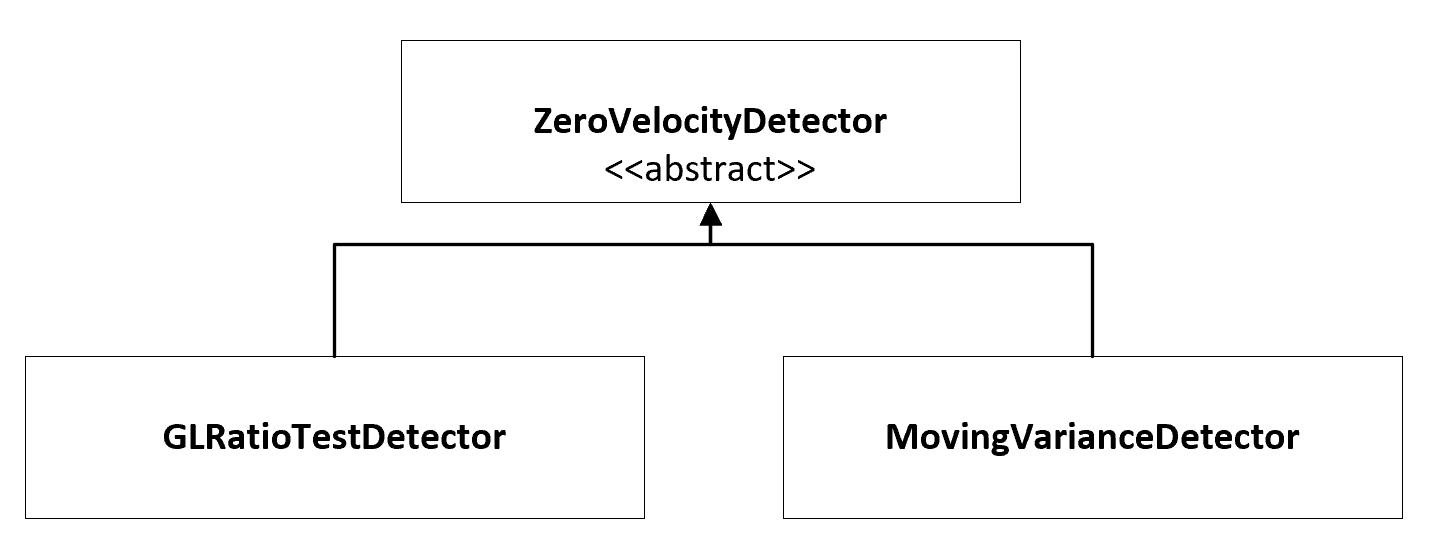
\includegraphics[width=\textwidth]{TESIS/imagenes/chap05/detectors-hierachy.PNG}
\caption{Componentes de deteccion de velocidad cero. Superclase abstracta ZeroVelocityDetector, subclases GLRatioTestDetector y MovingVarianceDetector.}
\label{FIG: Arquitectura2}
\end{figure}

\noindent Así pues, se emplearon dos estructuras de datos auxiliares. Primero, una cola FIFO del tamaño $W$ implementada con la estructura de datos LinkedList, destinada a almacenar las mediciones recepcionadas por el detector. Segundo, un arreglo de estados booleanos del mismo tamaño, que permite almacenar e iterar sobre los resultados de los tests estadísticos.

\noindent Cuando el ZVD detecta un nuevo evento de medición, en orden de precedencia ocurren los siguientes pasos dentro del detector:
\begin{enumerate}
    \item El sistema almacena la nueva medición en la cola FIFO
    \item Chequea si la cantidad de elementos de la cola es igual al tamaño de la ventana $W$ (caso base de primer procesamiento). Esto es, recopila los datos necesarios para el primer procesamiento, luego, a medida que llegan mediciones se agregan y se remueven elementos -el número de elementos es W-
    \item En caso de que la cola tenga $W$ observaciones, el detector procede a efectuar el test estadístico según el algoritmo ZVD seleccionado.
    \item Posterior, el resultado del test es almacenado en el arreglo de resultados de tal forma que:
    \begin{itemize}
        \item Si el test es positivo ($H_1$, es estacionario), todos los elementos del arreglo booleano se convierten en 1.
        \item Se obtiene y remueve el primer elemento del arreglo -primer test almacenado y actualizado W-1 veces dentro de la ventana W-.
        \item Se desplazan un lugar hacia la izquierda los restantes tests del arreglo (en inglés, left shift), y el último elemento $W-1$ es inicializado en 0 (i.e. $H_0$ o hipótesis nula).
    \end{itemize}
    \item Se despacha el resultado del test obtenido al listener u oyente del detector (en general, un analizador de datos), previamente establecido.
    \item Finalizado el procesamiento, en caso de que la cola de mediciones posea $W$ elementos, se remueve la primer medición y se continua iterando.
\end{enumerate}

Con el fin de clarificar las etapas mencionadas, se propone el pseudocódigo \nameref{pseudo-code-detectors}, sin embargo, no se refinan los metodos auxiliares empleados (e.g. makeTest, pushStatisticalTest).

\begin{algorithm}[H]
\caption{Pseudocódigo Zero Velocity Detector} \label{pseudo-code-detectors}
\begin{algorithmic}[1]
   \State Queue$<$MeasurementModel$>$ measures;
   \State Array$<$Boolean$>$ zupdtValues;
    \State W $\gets$  windowSize;
    \State setupParameters();
    \Statex
     \Function{updateDetector}{data}
        \State addQueue(measures,data);
    
        \If{sizeQueue(measures) == W} \Comment{PB. Espera por una ventana }

            \State boolean currentTest $\gets$  makeTest(); \Comment{Ejec. del test particular}

            \State int zValue $\gets$  pushStatisticalTest(currentTest); 
               
            \State removeQueue(measures);
            \State dispatchEventDetected(zValue); 
        \EndIf

    \EndFunction
    \Statex
     \Function{pushStatisticalTest}{test}
    
        \Comment{Actualizar la secuencia}
        \If{isH1 (test)} 
            \State setOnes(zupdtValues); \Comment{Establecer ventana en unos}
        \EndIf
        \Comment{shift data}
        \State z $\gets$ zupdtValues[0];
        \Comment{Shift 1 elemento a la izquierda}
        \ForAll{zupdtValues - 1}
           \State zupdtValues[i] $\gets$ zupdtValues[i+1];
        \EndFor
        \Comment{Próximo test en 0}
        \State zupdtValues[windowsSize-1] = 0;
        \Return{z};
   \EndFunction
\end{algorithmic}
\end{algorithm}

% Como 2.3 Presentar Algoritmo  Kalman Filter y Parámetros espacio-temporales
\section{Algoritmo Filtro de Kalman PARKIBIP}

A modo introductorio, en el capitulo \nameref{chap:project}, apartado \nameref{section:kalman-filter}, se presentó un algoritmo óptimo de estimación denominado filtro de Kalman; el cual sirve para poder identificar el estado oculto -no medible- de un sistema dinámico lineal que está sometido a ruido blanco Gausseano -cuya función de densidad responde a una distribución normal-. Es decir, permite hallar la mejor estimación de variables de interés no medibles (e.g. velocidad), a partir de la combinación de variables indirectas que son medibles (e.g. aceleración). Asimismo, con la finalidad de introducir a la temática se mencionaron brevemente algunas de sus aplicaciones, siendo en ciertos casos, el problema de estimar la posición de un sistema de navegación de un automóvil en movimiento similar al modelo empleado en PARKIBIP.

Análogo a lo sucedido con la estimación de la orientación en \nameref{impl:orientation-filter}, no se encontró una librería de código abierto que se adecue al contexto de PARKIBIP, y por consiguiente pueda ser reutilizada. 

Por lo tanto, se implementó un filtro de Kalman avanzado y multidimensional, en notación matricial. El propósito de dicho filtro es estimar las variables indirectas posición, velocidad y ángulos de Euler en cada instante de tiempo, a partir de las variables acelerómetro, giroscopio y magnetómetro sensadas por el dispositivo IMU. Para llevar adelante esta tarea, se requieren conocimientos y funciones avanzadas en álgebra lineal (e.g. operaciones matriciales) y física (e.g. leyes mecánicas, rotaciones y traslaciones). Todas las operaciones auxiliares requeridas fueron implementadas en la API de algoritmos en \nameref{API-algoritmos}.

El filtro de Kalman es un método numérico Predictor-Corrector, explicito de un solo paso; es decir depende únicamente de la estimación del estado previo ($x_{k-1}$) para lograr predecir el siguiente estado ($x_{k}$). El procedimiento Predictor-Corrector comienza mediante una primera predicción de los valores de las variables -resultantes de la extrapolación de una función ajustada (e.g. leyes mecánicas)-, luego, el corrector, refina la aproximación inicial utilizando el valor predicho de la función y una función objetivo que minimiza el error cuadrático medio del problema en cuestión.

Dada la complejidad del análisis, se deducen las ecuaciones físico-matemáticas y la metodologıa numérica empleada, así como un pseudo-código de la resolución de Kalman Filter con actualizaciones de cero velocidad.

\noindent Sea el \textbf{vector de estado} $\boldsymbol{x_k}$ en la iteración $\boldsymbol{k}$, dado por:

\[\left\{ 
            \begin{matrix*}[l]
            x_{k} = [P_k,V_k,O_k] = [position, velocity, orientation]\\
            P_k = (p_0,p_1,p_2),  p_i \in R \\
            V_k = (v_0,v_1,v_2), v_i \in R \\
            O_k = (roll,pitch,yaw),  o_i \in R
            \end{matrix*}
\right. \]

\noindent Previo a introducir el procedimiento del algoritmo, es imprescindible presentar los \textbf{Coeficientes} que intervienen en el formulamiento del filtro de Kalman y los roles que cumplen:

\begin{align*}
    F &= \text{Matriz Predicción o Transición} \\
    B &= \text{Matriz de Control} \\
    u &= \text{Vector de Control} \\
    P &= \text{Matriz de error de Covarianza de Estado} \\
    H &= \text{Matriz de Medición o relación entre mediciones y el vector de estado} \\
    R &= \text{Matriz de error de Covarianza Ruido de Medición} \\
    Q &= \text{Matriz de error de Covarianza Ruido del proceso} \\
\end{align*}

\noindent Aplicando las ecuaciones dadas por las \textbf{leyes mecánicas del movimiento} tanto para la posición como para la velocidad en función de la aceleración -medida por el sensor inercial- y el tiempo, se obtiene la siguiente formulación:

\[ 
x_k =\begin{bmatrix}
P_k\\
V_k
\end{bmatrix} = \begin{bmatrix}
P_{k-1} + V_{k-1}\Delta t +\frac{\Delta t^2}{2} \\
V_{k-1} + acc\Delta t
\end{bmatrix}
\]  


\noindent Reordenando los términos en función del vector de estados:
\begin{equation}
    x_k = \begin{pmatrix}
              1 & \Delta t\\ 
                 0 & 1
            \end{pmatrix} X_{k-1} +
            \begin{pmatrix}
  \frac{\Delta t^2}{2}\\ 
  \Delta t
\end{pmatrix} acc
\end{equation}  

\begin{equation}
     x_k = F X_{k-1} + B u
\end{equation}

\noindent Definiendo los cambios de variables, hallamos los valores \textbf{F} = $\begin{pmatrix}
              1 & \Delta t\\ 
                 0 & 1
            \end{pmatrix}$, \textbf{B} =$\begin{pmatrix}
  \frac{\Delta t^2}{2}\\ 
  \Delta t
\end{pmatrix}$ y $\boldsymbol{u_{k-1}}$ = acc. 

Finalmente, Se logra obtener un método iterativo para predecir las ecuaciones de navegación o transición de estados, que puede ejecutarse en tiempo real a medida que se recopilan los datos de medición.

\noindent Entonces, para el paso (i), se llama $\hat{x_{k}}$ y $\hat{P_k}$ las variables estimadas en la predicción y sus ecuaciones vienen dadas por:
\[ (i) \boldsymbol{Predicci\Acute{o}n}\left\{ 
            \begin{matrix}
            \hat{x_{k}} = F X_{k-1} + B u_{k-1} + w_{k-1} \\
            \hat{P_k} = FP_{k-1}F^t + Q\\
             u_{k-1}=(accX,accY,accZ)
            \end{matrix}
\right. \]

\noindent Luego, en (ii), se ejecuta la actualización de los valores estimados mediante la aplicación del factor de ganancia de Kalman. Primero, calcula el factor de ganancia $K$, corrige el estado con la medición, actualiza la matriz de Covarianza. Esto es:
\[ (ii) \boldsymbol{Correcci\Acute{o}n}\left\{ 
            \begin{matrix}
            K_k = \frac{\hat{P_k}H^t}{H.\hat{P_k}H^t + R}\\
            y_k = H\hat{x_{k}} +v_k\\
            x_{k} =  \hat{x_{k}} + K_k y_k\\
            P_k = (I -K_k.H)\hat{P_k}
            \end{matrix}
\right. \]

%TODO: no hay referencia a esta imagen 
\begin{figure}[H]
    \centering
    \captionsetup{justification=centering}
    \resizebox{\textwidth}{!}{
    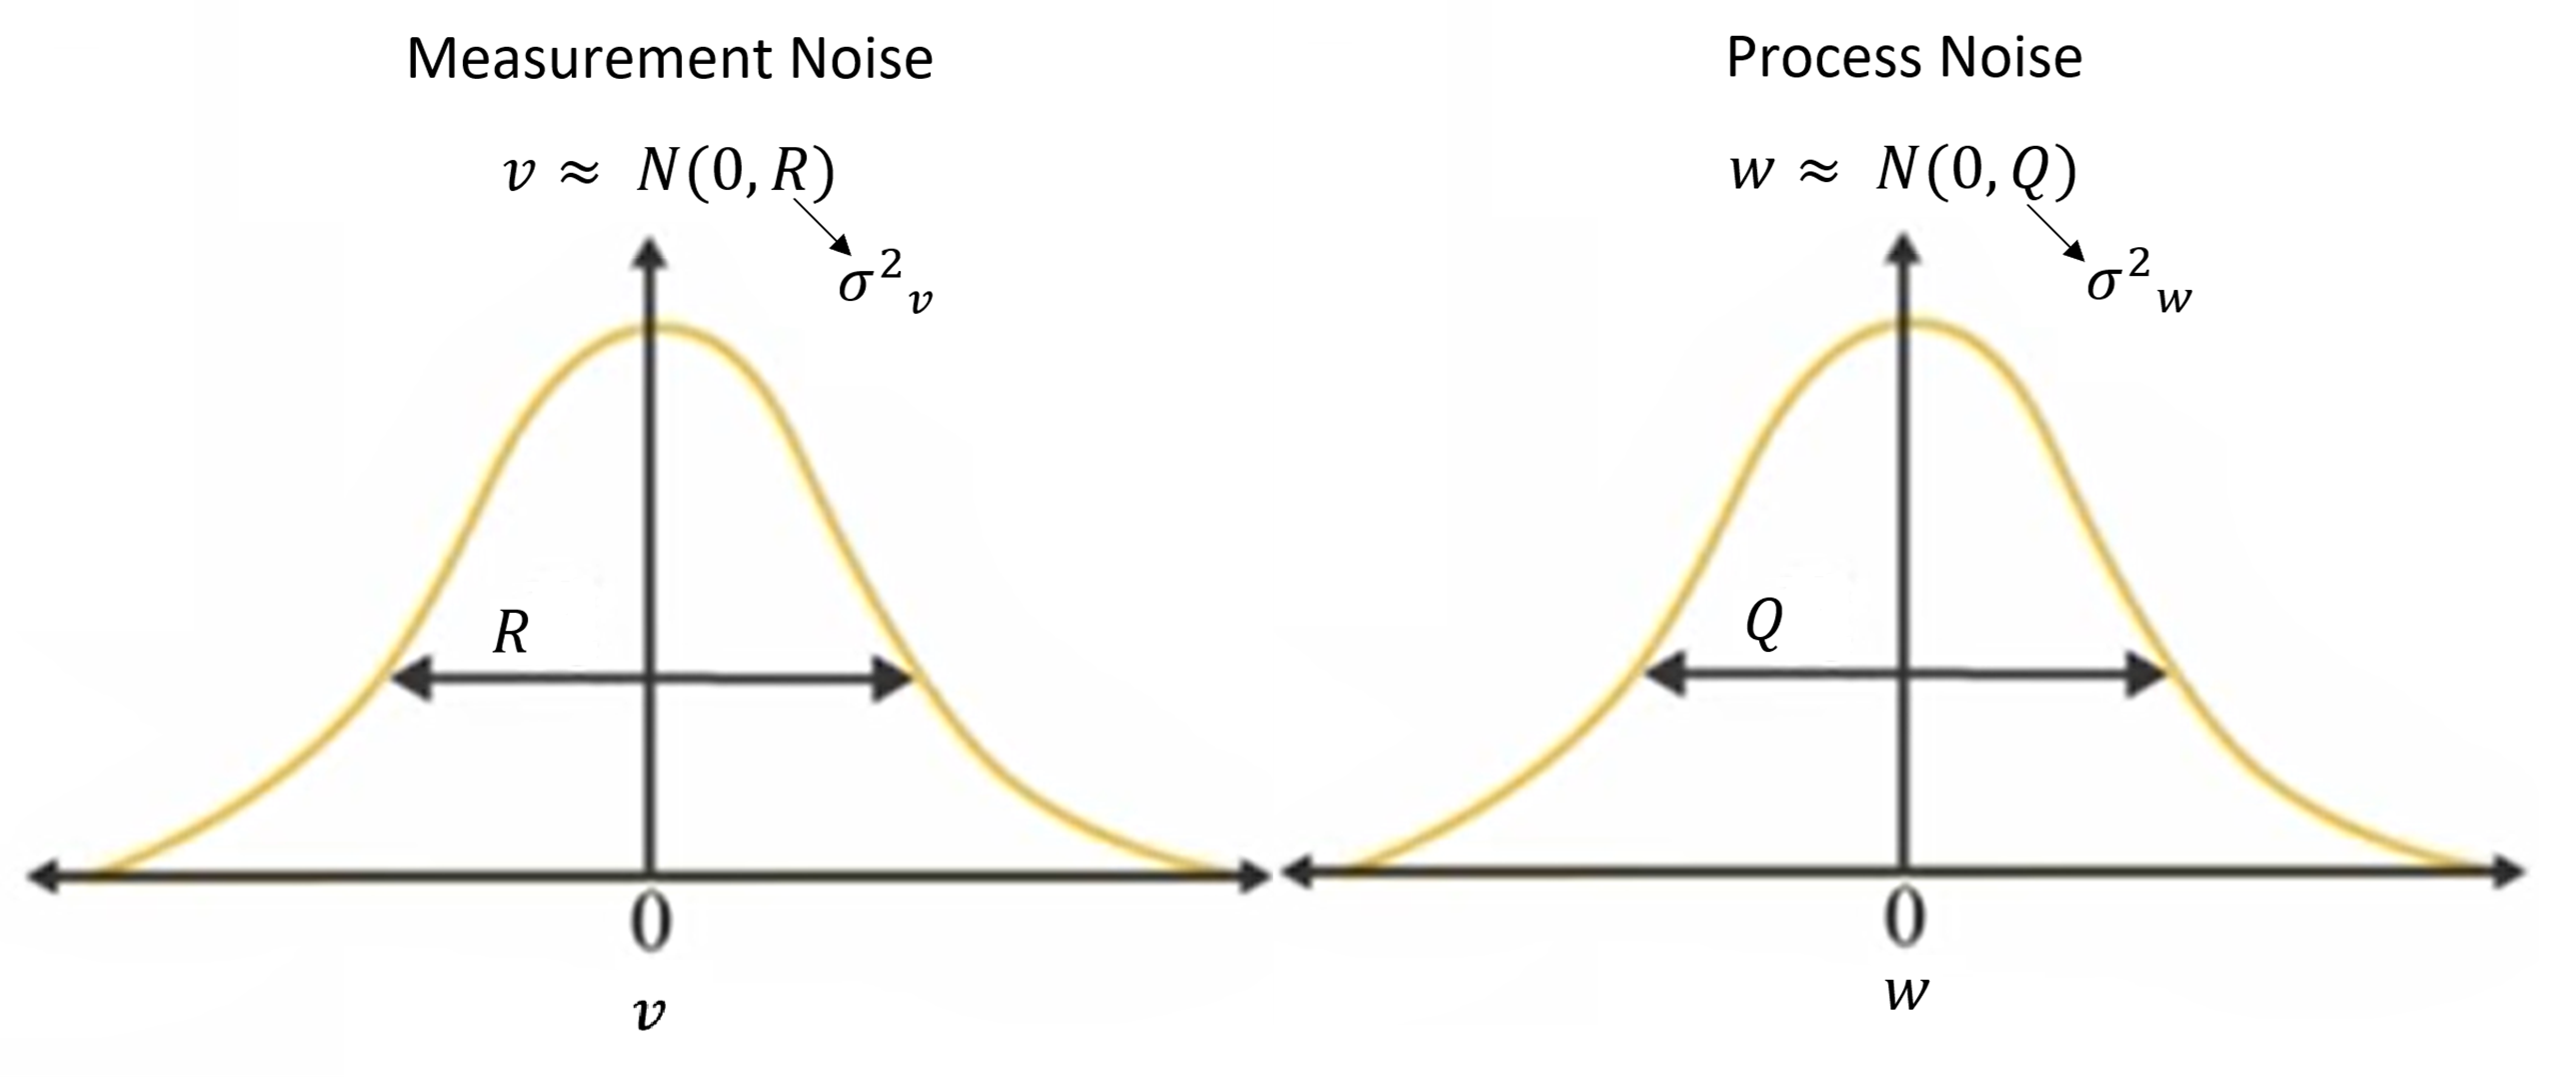
\includegraphics{TESIS/imagenes/chap05/kalman-noises.PNG}}
    \caption{Distribuciones supuestas para los vectores de ruido estadísticos de Medición $v_k$ y de Proceso $w_k$.}
    \label{FIG: madgwick}
\end{figure}

El sistema de ecuaciones debe contemplar los desvíos relacionados a los distintos ruidos estadísticos. Para esto, se asume que los vectores $v_k$ y $w_k$ de ruido de medición y proceso poseen una distribución gaussiana de media cero y covarianzas R y Q respectivamente. Las matrices Q y R en general se emplean como parámetros de ajuste para obtener el rendimiento deseado.

Una particularidad crucial del modelo empleado, es la integración del método Zero Velocity al filtro de Kalman. Esta tarea permite \underline{compensar la velocidad} en la etapa de corrección (ii), llevando su valor a Cero en caso de que el algoritmo Zero Velocity Detector identifique un momento estacionario. Así, se reducen considerablemente los desvíos incrementales debido al error acumulativo de integración respecto al tiempo.

\begin{algorithm}[H] 
\caption{Pseudocódigo de Kalman Filter con compensacion Zero Velocity} \label{pseudo-code-kf}
\begin{algorithmic}[1]
    \Function{initKalmanFilterZUpdtate}{A}  
        \State initFilters();
        \State initVectors();
    \EndFunction
    \Statex
     \Function{runKalmanFilterZUpdtate}{$measure_k, zValue_k$}
        \Statex
        \Comment{\textbf{Prediction with previous $x_h$}}
        \State xhat $\gets$ NavigationEquations($measure_k, x_h$);
        \Statex
         \Comment{\textbf{Compute F and G}}
        \State stateMatrix($measure_k$); 
        \Statex
        \Comment{\textbf{Predict state covariance matrix $P=F*P*F'+G*Q*G'$;}}
        \State P$\gets$F.multiply(P).multiply(F.transpose()).add(G.multiply(Q).multiply(G.transpose())); 
        
        \Comment{\textbf{Check covariance matrix P is symmetric}}
        \State P $\gets$ P.add(P.transpose()).scalarMultiply(0.5d);
        
        \Statex
        \Comment{\textbf{Check if a zero velocity update should be done}}
        \If{$zValue == true$}

                \Statex 
                \Comment{\textbf{K=(P*H')/(H*P*H'+R); s = H*P*H'+R, solve s'.k'=H.P'}}
                \State RealMatrix s $\gets$ H.multiply(P).multiply(H.transpose()).add(R);
                \State RealMatrix b $\gets$ H.multiply(P.transpose());
                \State RealMatrix K$\gets$new CholeskyDecomposition(s.transpose()).solve(b).transpose();

               \Statex
               \Comment{ \textbf{Innovation z=-x}}
               \State RealVector innovation $\gets$ H.operate(xhat).mapMultiply(-1);

               \Comment{\textbf{Correct xhat using the estimated perturbations}}
               \State RealVector dx $\gets$ K.operate(innovation);
               \State $x_h$ $\gets$ xhat.add(dx);
               
               \Statex \Comment{\textbf{Compensate current orientation}}
               \State compensateOrientation(dx);
               
               \Statex
               \Comment{\textbf{Compensate current covariance matrix P}}
               \State P = Id.subtract(K.multiply(H)).multiply(P);
               
               \Statex
               \Comment{\textbf{Check covariance matrix P is symmetric}}
               \State P $\gets$ P.add(P.transpose()).scalarMultiply(0.5d);

        \Else
            \State $x_h$ $\gets$ xhat; \Comment{\textbf{Update new $x_h$ if not correction is done}}
        \EndIf

    \EndFunction

\end{algorithmic}
\end{algorithm}
 
Para concluir con la exposición de el filtro de Kalman integrado a un detector de cero velocidad, se expone el \textbf{pseudo-código} de la implementación realizada en el lenguaje Java de Android dado por \nameref{pseudo-code-kf}. El filtro se inicializa mediante la función ``initKalmanFilterZUpdate'', luego con la recepción de cada medición se ejecuta la función ``runKalmanFilterZUpdate''.

Los valores empleados para los coeficientes fueron elegidos acorde a la especificación del hardware y para optimizar el funcionamiento de la aplicación. A continuación, se exponen las configuraciones para el ruido de proceso, el ruido de medición y matrices de covarianza de estado inicial Q, R y P. Se supone que las tres matrices son matrices diagonales y todas las configuraciones se definen como desviaciones estándar:

\begin{itemize}
    \item Período de muestreo del sistema:
    \begin{itemize}
        \item Ts [seg]= (1/f), f frecuencia configurable 
    \end{itemize}
    \item Ruido de proceso para modelar el ruido del acelerómetro (eje de coordenadas x, y, z) y otros errores del acelerómetro:
    \begin{itemize}
        \item Ruido de Aceleración[m/$s^2$]: sigmaAcc = $0.5^{2}$
    \end{itemize}
    \item Ruido de proceso para modelar el ruido del giroscopio (eje de coordenadas x, y, z) y otros errores del giroscopio:
    \begin{itemize}
        \item Ruido Angular[rad/s]: sigmaGyro = $(0.5*pi/180)^{2}$ 
    \end{itemize}
    \item Elementos diagonales de la matriz de Covarianza P del estado inicial:
     \begin{itemize}
        \item Varianza de Posición [m]: sigmaP = $(1\cdot10^{-5})^{2}$ 
        \item Varianza de Velocidad [m/s]: sigmaV = $(1\cdot10^{-5})^{2}$
        \item Varianza de Orientación [rad]: sigmaAtt = $(pi/180*0.1)^{2}$
        \item Desviación de Aceleración[m/$s^2$]: sigmaA =$(0.3)^{2}$
        \item Desviación de Velocidad angular [rad/s]: sigmaG = $(0.*pi/180)^{2}$ 
    \end{itemize}
    \item Covarianza de ruido de medición R:
    \begin{itemize}
        \item Desviación de Velocidad sigmaVelR [m/s] =0.01
    \end{itemize}
    
\end{itemize}

El vector de estados se inicializa mediante un \textbf{Procedimiento de Calibración}. El mismo consiste en recopilar las primeras N = 30 observaciones del sistema, computar la media de las variables roll, pitch, yaw; luego establecer el vector de estados. La posición y la velocidad inicial comienza con el valor 0:
\begin{equation*}
    X_{initial}= \begin{pmatrix}
0&0&0&0&0&0& \bar{roll}& \bar{pitch}& \bar{yaw}
\end{pmatrix}
\end{equation*}

Los coeficientes estables del sistema dinámico P (inicial), Q, H, R, fueron establecidos de la siguiente manera:
\begin{equation*}
    P_{initial}  = \begin{pmatrix}
sigmaP&0&0&0&0&0&0&0&0\\    
0&sigmaP&0&0&0&0&0&0&0\\
0&0&sigmaP&0&0&0&0&0&0\\
0&0&0&sigmaV&0&0&0&0&0\\
0&0&0&0&sigmaV&0&0&0&0\\
0&0&0&0&0&sigmaV&0&0&0\\
0&0&0&0&0&0&sigmaAtt&0&0\\
0&0&0&0&0&0&0&sigmaAtt&0\\
0&0&0&0&0&0&0&0&sigmaAtt
\end{pmatrix} 
\end{equation*}
\begin{equation*}
% %//6x6
Q  = \begin{pmatrix}
sigmaAcc&0&0&0&0&0\\    
0&sigmaAcc&0&0&0&0\\
0&0&sigmaAcc&0&0&0\\
0&0&0&sigmaGyro&0&0\\
0&0&0&0&sigmaGyro&0\\
0&0&0&0&0&sigmaGyro
\end{pmatrix}
\end{equation*}

\begin{equation*}
% %//3x9
H  = \begin{pmatrix}
0&0&0&1&0&0&0&0&0\\    
0&0&0&0&1&0&0&0&0\\
0&0&0&0&0&1&0&0&0\\
\end{pmatrix}
\end{equation*}

\begin{equation*}
%% 3*3
R  = \begin{pmatrix}
sigmaVelR&0&0\\
0&sigmaVelR&0\\
0&0&sigmaVelR
\end{pmatrix}
\end{equation*}
% $\in$ $M{9\times9}$

Los restantes valores -P, F, B, u-, mutan según las observaciones recopiladas en cada instante de tiempo y la dinámica del sistema. Se resalta la implementación de un algoritmo iterativo, que reacciona con cada evento de medición.

En orden de precedencia ocurren los siguientes eventos de sistema:
\begin{enumerate}
    \item Recopilación de mediciones: aceleración, velocidad angular, fuerzas magnéticas
    \item Estandarización de unidades inerciales sobre las mediciones
    \item Computo de la orientación instantánea en formato cuaternión -a partir de los datos medidos- mediante filtro eficiente de orientación
    \item Con la orientación adquirida. Rotación a un marco de referencia inercial -tierra-, desde el marco del sensor
    \item Ejecución de algoritmo Zero Velocity Detector
    \item Ejecución del filtro de Kalman con los datos procesados -cuaternión, mediciones, zero velocity-
\end{enumerate}

\newpage

\section{Analizadores de datos} 

Los analizadores de datos son las entidades que tienen por misión procesar los datos crudos que provienen desde los distintos sensores del IMU, utilizando los métodos numéricos ya mencionados (e.g detección de velocidad cero, filtrado de Kalman, entre otros). Son representados en el sistema mediante la clase \textit{DataAnalyzer}. El diseño de clases de esta sección del sistema se puede ver en la figura Fig. \ref{FIG:data-analyzer-class-diagram}. 

\begin{figure}[H]
    \hspace*{-3.0cm}%
    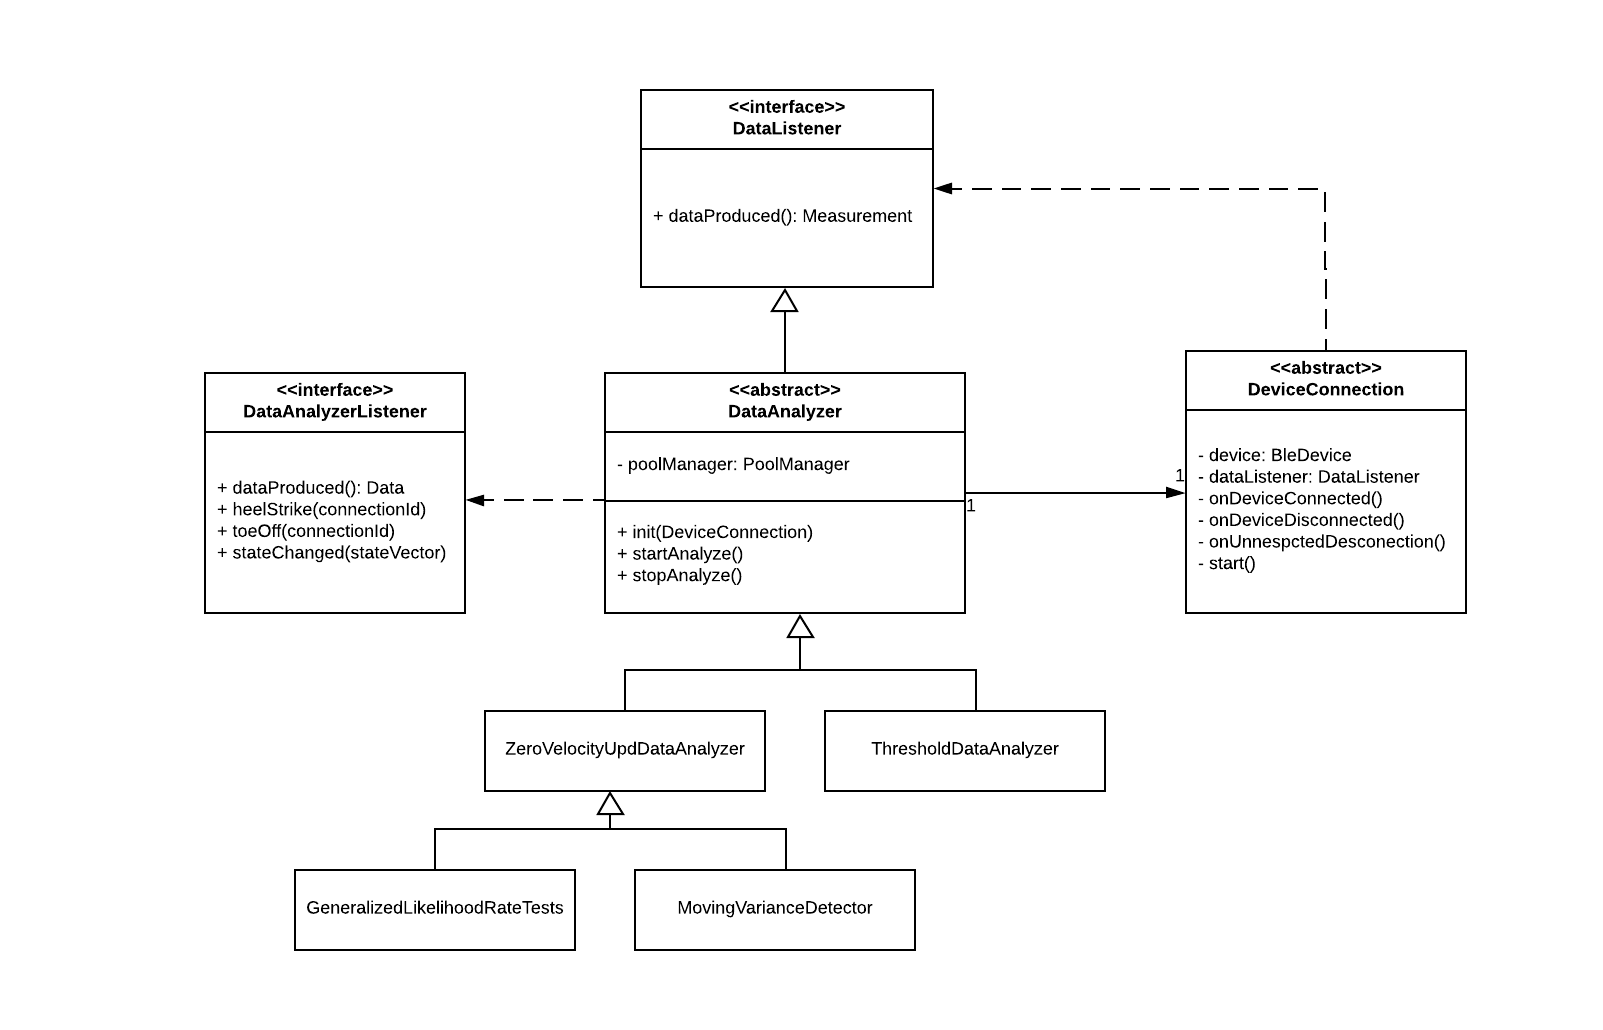
\includegraphics[clip,width=1.3 \columnwidth]{TESIS/imagenes/chap05/data-analyzers-class-diagram.png}    
    \caption{Diagrama de clases del módulo de la aplicación Android en donde se analizan y procesan los datos para detectar eventos relativos a la marcha del paciente.}
    \label{FIG:data-analyzer-class-diagram}
\end{figure}

Tal como se puede apreciar en la figura, el \textit{DataAnalyzer} implementa la interfaz \textit{DataListener}, y así, posee la capacidad de recibir los datos desde una instancia de \textit{DeviceConnection} -entidad que representa una conexión con un dispositivo IMU-. Es decir, cada \textit{DeviceConnection} tiene asociado un \textit{DataAnalyzer}, definido como su \textit{DataListener}. Cuando es invocado el método \textit{startAnalyze()} correspondiente a un analizador, éste le comunica a su \textit{DeviceConnection} que puede comenzar el flujo de datos. La instancia de \textit{DeviceConnection} inicia el envío de datos de medición, representados con el modelo \textit{Measurement}, a través de la interfaz \textit{DataListener}, para que el analizador de datos pueda procesar las mediciones producidas por los sensores. 

Existen diferentes \textit{DataAnalyzers} en la aplicación. Cada uno implementa un método numérico particular para analizar los datos. Durante el diseño se utilizó el concepto de polimorfismo; es decir, el comportamiento de todos los \textit{DataAnalyzers} se encuentra definido en ésta clase abstracta, sin embargo, cada instancia concreta implementa los métodos derivados de forma particular empleando diferentes métodos numéricos. Por ejemplo, \textit{ZeroVelocityUpdateDataAnalyzer} implementa el método de detección de velocidad cero para procesar los datos e identificar los eventos Heel Strike y Toe Off. 

El hecho de utilizar polimorfismo para los analizadores de datos hace que el sistema sea escalable y extensible, ya que implementar un nuevo método para analizar los datos y generar eventos, implica crear únicamente una clase concreta que extienda de la clase \textit{DataAnalyzer}. Además, cada analizador desarrolla un único método de análisis y tiene asignada una única responsabilidad bien definida. Este forma de diseño, contribuye a mejorar la calidad del sistema, haciendo que sea más sencillo realizar pruebas sobre un método de análisis concreto y compararlo con el resto de los métodos; además de incrementar su mantenibilidad. 
Cuando un \textit{DataAnalyzer} detecta eventos u obtiene nuevos datos como resultado, los envía a su \textit{DataAnalyzerListener}. Esta interfaz está definida para ser implementada por la entidad que esté interesada en recibir el resultado del procesamiento, que en la implementación final de PARKIBIP esta entidad es \textit{BiofeedbackModule}. 

\textit{DataAnalyzerListener} es un protocolo definido para ser implementados por las entidades que necesiten observar los resultados de un \textit{DataAnalyzer}. Cuando un analizador de datos detecta cierto evento de la marcha, notifica a su \textit{DataAnalyzerListener}. En PARKIBIP, este protocolo es implementado por \textit{BiofeedbackModule}.

\section{Configuración de algoritmos y parámetros} 

PARKIBIP es también una aplicación experimental. Es decir, si bien el objetivo principal es obtener un sistema que beneficie la marcha de los enfermos de Parkinson; pretende ser, en una primera instancia, una herramienta de investigación que permita encontrar la mejor forma de estimular a un paciente para que su marcha progrese. Por lo tanto, resulta crucial experimentar con los algoritmos desarrollados para estudiar la marcha, poder utilizar un método u otro, configurar éstos métodos numéricos de distintas formas, establecer distintas reglas para definir los estímulos, etc. 

Ante ésta necesidad, se desarrolló un modulo de configuración. Este módulo consta de su propia interfaz gráfica, la cual puede ser encontrada dentro del menú principal de la aplicación. En la figura Fig. \ref{FIG:configuration-class-diagram}, se expone el diagrama de clases correspondiente a la porción del sistema dedicada a la parametrización.

\newpage

\begin{figure}[H]
    \hspace*{-3.5cm}%
    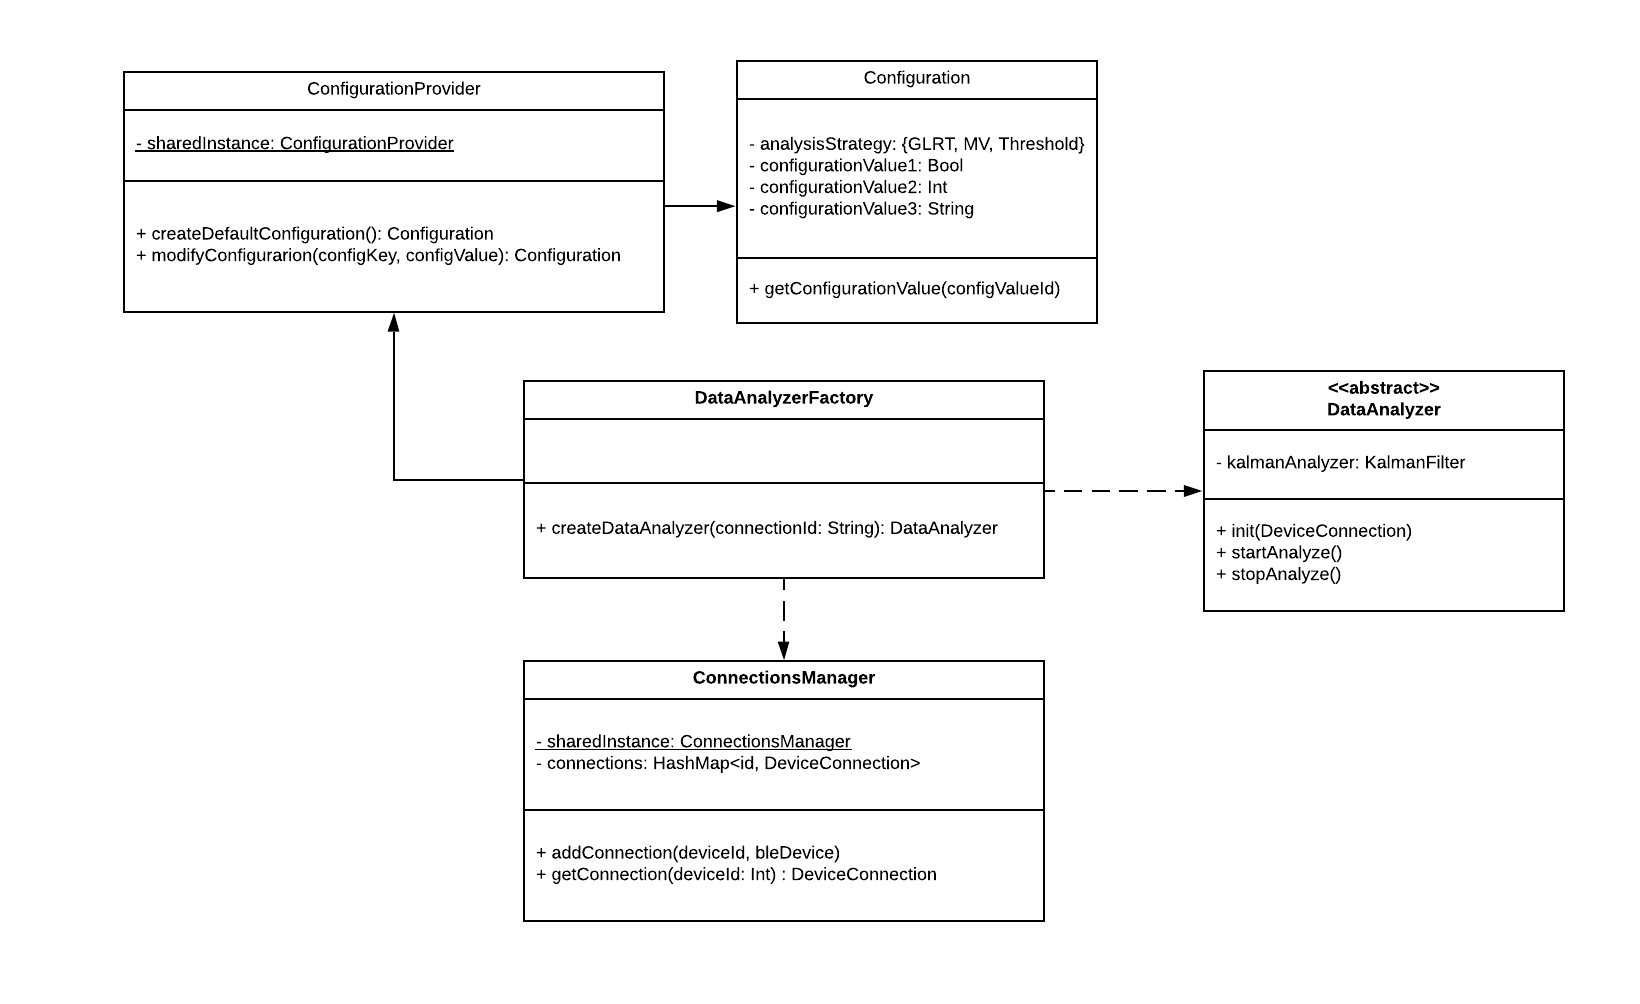
\includegraphics[clip,width=1.4 \columnwidth]{TESIS/imagenes/chap05/configuration-class-diagram.png}    
    \caption{Diagrama de clases del módulo de la aplicación Android donde se administran las distintas configuraciones del sistema}
    \label{FIG:configuration-class-diagram}
\end{figure}

Un estado de configuración está representado por una instancia de la clase \textit{Configuration}. La misma clase, dispone del conjunto de atributos correspondientes a cada uno de los parámetros que pueden ser editados dentro del sistema. A su vez, \textit{ConfigurationProvider} es la clase encargada de manejar éstas configuraciones, por ende, un objeto \textit{Configuration} se mantiene inmutable mientras el proveedor no ejecute una transacción de modificación sobre el mismo. Cuando un valor es modificado a través de la pantalla de Configuraciones de la aplicación, esta \textit{Activity} invoca al proveedor de configuraciones para solicitarle dicho cambio.

\textit{ConfigurationProvider} implementa el patrón de diseño \textit{Singleton}, es decir, una clase para la cual existe una única instancia, y una vez creada se mantiene en memoria durante todo el ciclo de vida de la aplicación Android. Este \textit{Singleton} mantiene una referencia a la instancia de \textit{Configuration} actual, y al ser global, puede ser accedido desde cualquier clase del sistema. 

El rol principal del módulo de configuraciones, es el de proveer los parámetros necesarios para configurar los métodos numéricos pertenecientes a los analizadores de datos. Cuando se desea crear un analizador de datos -\textit{DataAnalyzer}-, el método \textit{createDataAnalyzer(DeviceConnection)} de la fábrica de datos  \textit{DataAnalyzerFactory} es invocado. De esta forma, éste patrón ``factory'', puede crear instancias de \textit{DataAnalyzer} vinculadas a la conexión con el dispositivo que le fue provista por parámetro, a partir de la configuración actual. Esto es, le solicita al proveedor \textit{ConfigurationProvider} la configuración vigente y construye el \textit{DataAnalyzer} adecuado empleando los parámetros de la misma. Esta configuración, indica cuál es el \textit{DataAnalyzer} que debe ser creado, según el método de análisis seleccionado por el Usuario, así como sus parámetros requeridos para establecer éste método. 

Dentro de los posibles parámetros que se pueden configurar en esta sección de la aplicación se encuentran:

\begin{enumerate}
    \item Algoritmo de detección de fases de la marcha:
    \begin{itemize}
        \item Threshold: Algoritmo básico de detección de eventos a partir de picos de aceleración. 
        \item Acceleration Moving Variance Detector: Algoritmo de detección de eventos a partir de la detección de momentos de velocidad cero -ver \ref{base-detectors}-.
        \item Generalized Likelihood Ratio Test: Algoritmo de detección de eventos a partir de la detección de momentos velocidad cero -ver \ref{base-detectors}-.
    \end{itemize}
    \item Parámetros globales que afectan a todos los métodos implementados:
    \begin{itemize}
        \item Gravity: Valor de la aceleración gravitatoria \(\frac{m}{s^2}\).
        \item Windows size: Tamaño de la ventana de mediciones contiguas a ser analizadas por los métodos para la detección de eventos. 
        \item Accelerometer frequency: Frecuencia configurada en el acelerómetro para recopilación de mediciones del sensor, expresada en la unidad Hz.
        \item Gyroscope frequency: Frecuencia configurada en el giroscopio para enviar las mediciones, expresada en la unidad Hz. 
    \end{itemize}
    \item Reglas de biofeedback, para decidir cuándo se debe estimular al Paciente.
    \item Activación de tipos de estímulos: vibración y/o sonido.
    \item Coeficientes particulares de cada método.
\end{enumerate}

En la pantalla de configuración -ver Fig. \ref{fig:activity-configuration}-, representada con la clase \textit{ConfigurationActivity}, se implementó adicionalmente la posibilidad de re-establecer la configuración por defecto. Esto permite que, luego de realizar ciertos experimentos al cambiar los parámetros, se pueda volver a la configuración de fábrica (i.e. considerados valores óptimos de PARKIBIP). Esta funcionalidad es de vital importancia si se quiere rápidamente re-establecer la configuración sin necesidad de obtenerla nuevamente, o de realizar una reinstalación de la aplicación. Además, durante un proceso de edición de parámetros, se le permite al usuario descartar los cambios realizados, retornando a su estado inicial. Estas funcionalidades se pueden ver con mayor detalle en la sección \nameref{chap:project-scope}.

\begin{figure}[!h]
     \centering
     \begin{subfigure}[t]{0.4\textwidth}
         \centering
         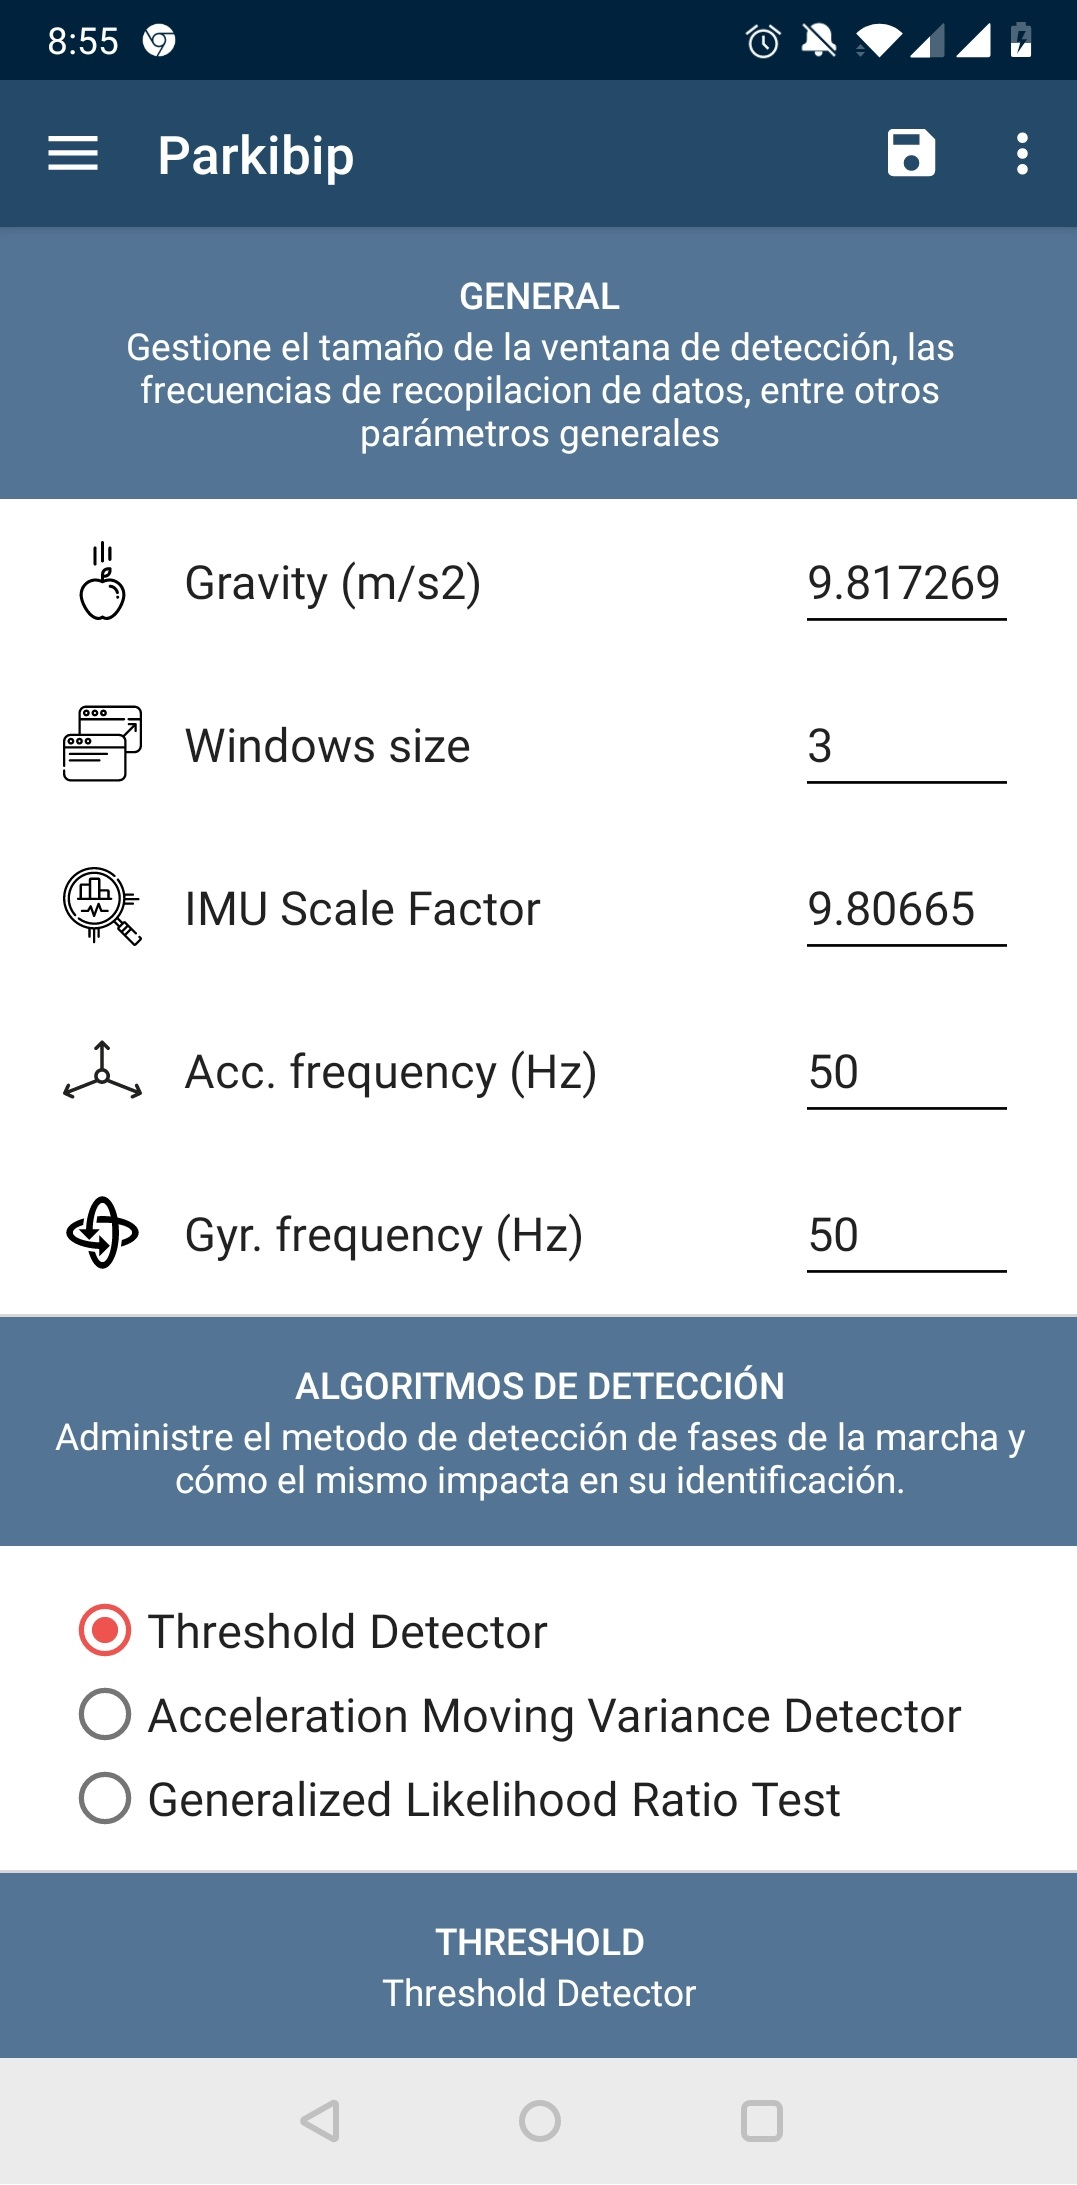
\includegraphics[height=8cm]{TESIS/imagenes/chap05/activity-configuration.JPG}
         \caption{Configuración de parámetros y selección del algoritmo de detección. PARKIBIP habilita al usuario a modificar parámetros generales y específicos de los métodos.}
     \end{subfigure}
     ~
     \begin{subfigure}[t]{0.4\textwidth}
         \centering
         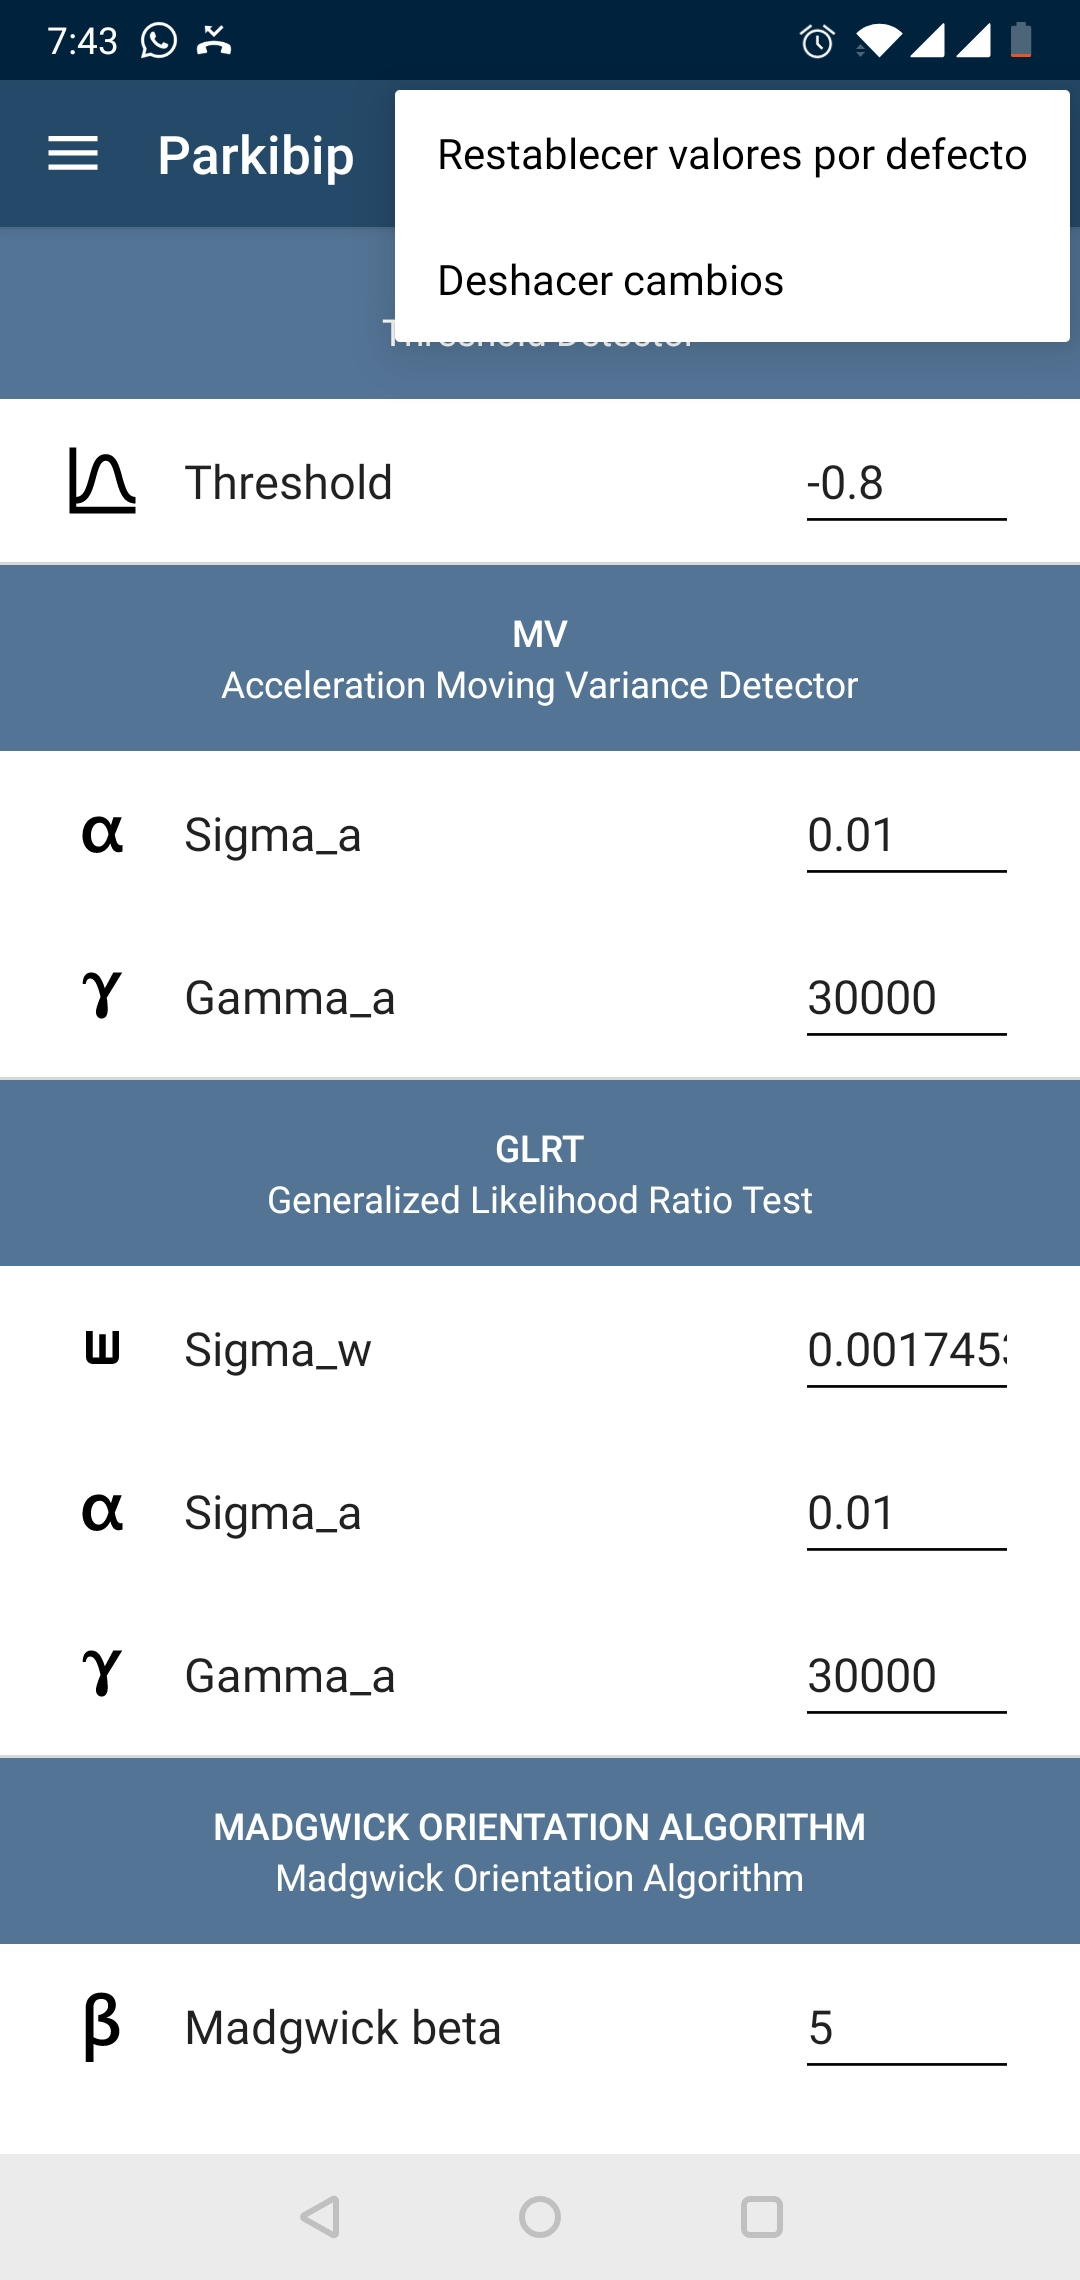
\includegraphics[height=8cm]{TESIS/imagenes/chap05/activity-configuration2.JPG}
         \caption{Restauración de valores. PARKIBIP permite restablecer a valores de fábrica, así como descartar cambios efectuados.}
     \end{subfigure}
     \caption{Configuración de parámetros generales y particulares a los detectores. Además, selección del algoritmo de detección.}
     \label{fig:activity-configuration}
 \end{figure}

\newpage

\section{Módulo de Biofeedback}

El módulo de \textit{Biofeedback} cumple una función esencial para PARKIBIP. Con una visión global, es el encargado de capturar y procesar los resultados de los distintos \textit{DataAnalyzer} -analizador creado para cada IMU-, los cuales procesan los datos, emiten eventos a dicho módulo -indicando la ocurrencia de un Heel Strike o un Toe Off- y además, notifican parámetros espacio-temporales como la posición, la velocidad y la orientación instantánea relativos a cada pie.  Así, el módulo de Biofeedback transforma la información recibida según reglas pre-definidas dentro del mismo, para estimular al usuario,  y luego calcula los datos de la sesión en tiempo real para ser mostrados en la pantalla. 

La figura Fig. \ref{FIG:biofeedback-module-class-diagram} presenta un diagrama del subsistema en el cual se encuentra el módulo de Biofeedback -representado con la clase \textit{BiofeedbackModule}-, donde se puede visualizar cuáles son las clases con las que el mismo interactúa.

\begin{figure}[H]
    \hspace*{-3.5cm}%
    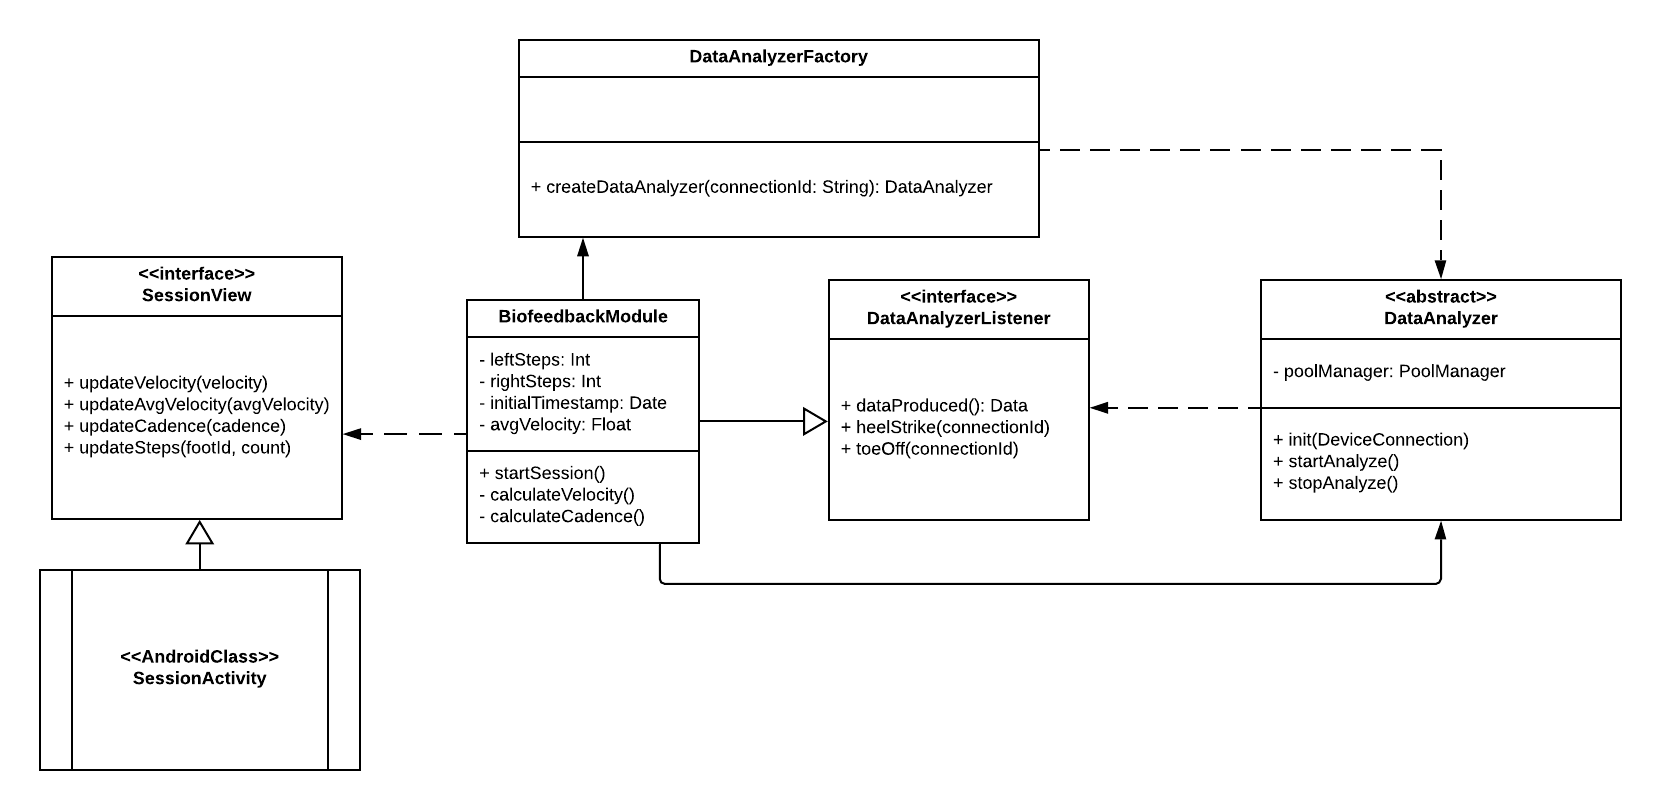
\includegraphics[clip,width=1.4 \columnwidth]{TESIS/imagenes/chap05/biofeedback-module-design.png}   
    \caption{Diagrama de clases del módulo de la aplicación Android que establece las reglas para estimular y calcula los parámetros espacio-temporales de la sesión en tiempo real}
    \label{FIG:biofeedback-module-class-diagram}
\end{figure}

Cuando es iniciada una sesión de fisioterapia con PARKIBIP, \textit{BiofeedbackModule} es quien solicita al \textit{DataAnalyzerFactory} la creación de los \textit{DataAnalyzer}, se suscribe a los eventos como su \textit{DataAnalyzerListener} manteniendo las referencias adecuadas. Para procesar los datos que produce cada \textit{DataAnalyzer}, implementa la interfaz \textit{DataAnalyzerListener}. Esta interfaz encapsula todos los métodos que utiliza el \textit{DataAnalyzer} para notificar a las clases interesadas los datos que obtiene como resultado del procesamiento. Así, los \textit{DataAnalyzer} notifican a su \textit{DataAnalyzerListener} cada vez que se produce un evento del tipo Heel Strike o Toe Off, como también las actualizaciones del vector de estado del algoritmo filtro de Kalman, el cual contiene posición, velocidad y orientación. 

\textit{BiofeedbackModule} emplea los entradas mencionadas para calcular los siguientes datos en tiempo real:

\begin{itemize}
    \item Velocidad instantánea para cada pie 
    \item Velocidad promedio de la marcha 
    \item Cantidad de pasos
    \item Cadencia (i.e pasos por minutos) 
    \item Duración media del paso 
    \item Aceleración instantánea para cada pie 
    \item Aceleración promedio de la marcha 
\end{itemize}

Este módulo, tiene además la capacidad de reaccionar a ciertas reglas pre-definidas y configurables conforme a estimular adecuadamente al paciente. Los niveles de estímulos para el paciente PARKIBIP son: 

\begin{itemize}
    \item Vibración en el dispositivo IMU utilizando el motor de vibración embebido en el dispositivo MetaMotionR.
    \item Sonido ``Beep'' emitido por la aplicación móvil, el cual es tan importante como para tener su referencia en el nombre del proyecto.
\end{itemize}

La figura Fig. \ref{fig:activity-active-session} ilustra una sesión PARKIBIP en curso. Tal como se puede apreciar, el sistema reacciona en tiempo real a la marcha del paciente en rehabilitación, mediante el envío de estímulos externos -vibración y/o sonido- y el cómputo de parámetros espacio-temporales. Así, medición a medición, la interfaz de usuario comienza a transitar por distintos valores fruto del procesamiento de PARKIBIP.  

\begin{figure}[H]
 \centering
 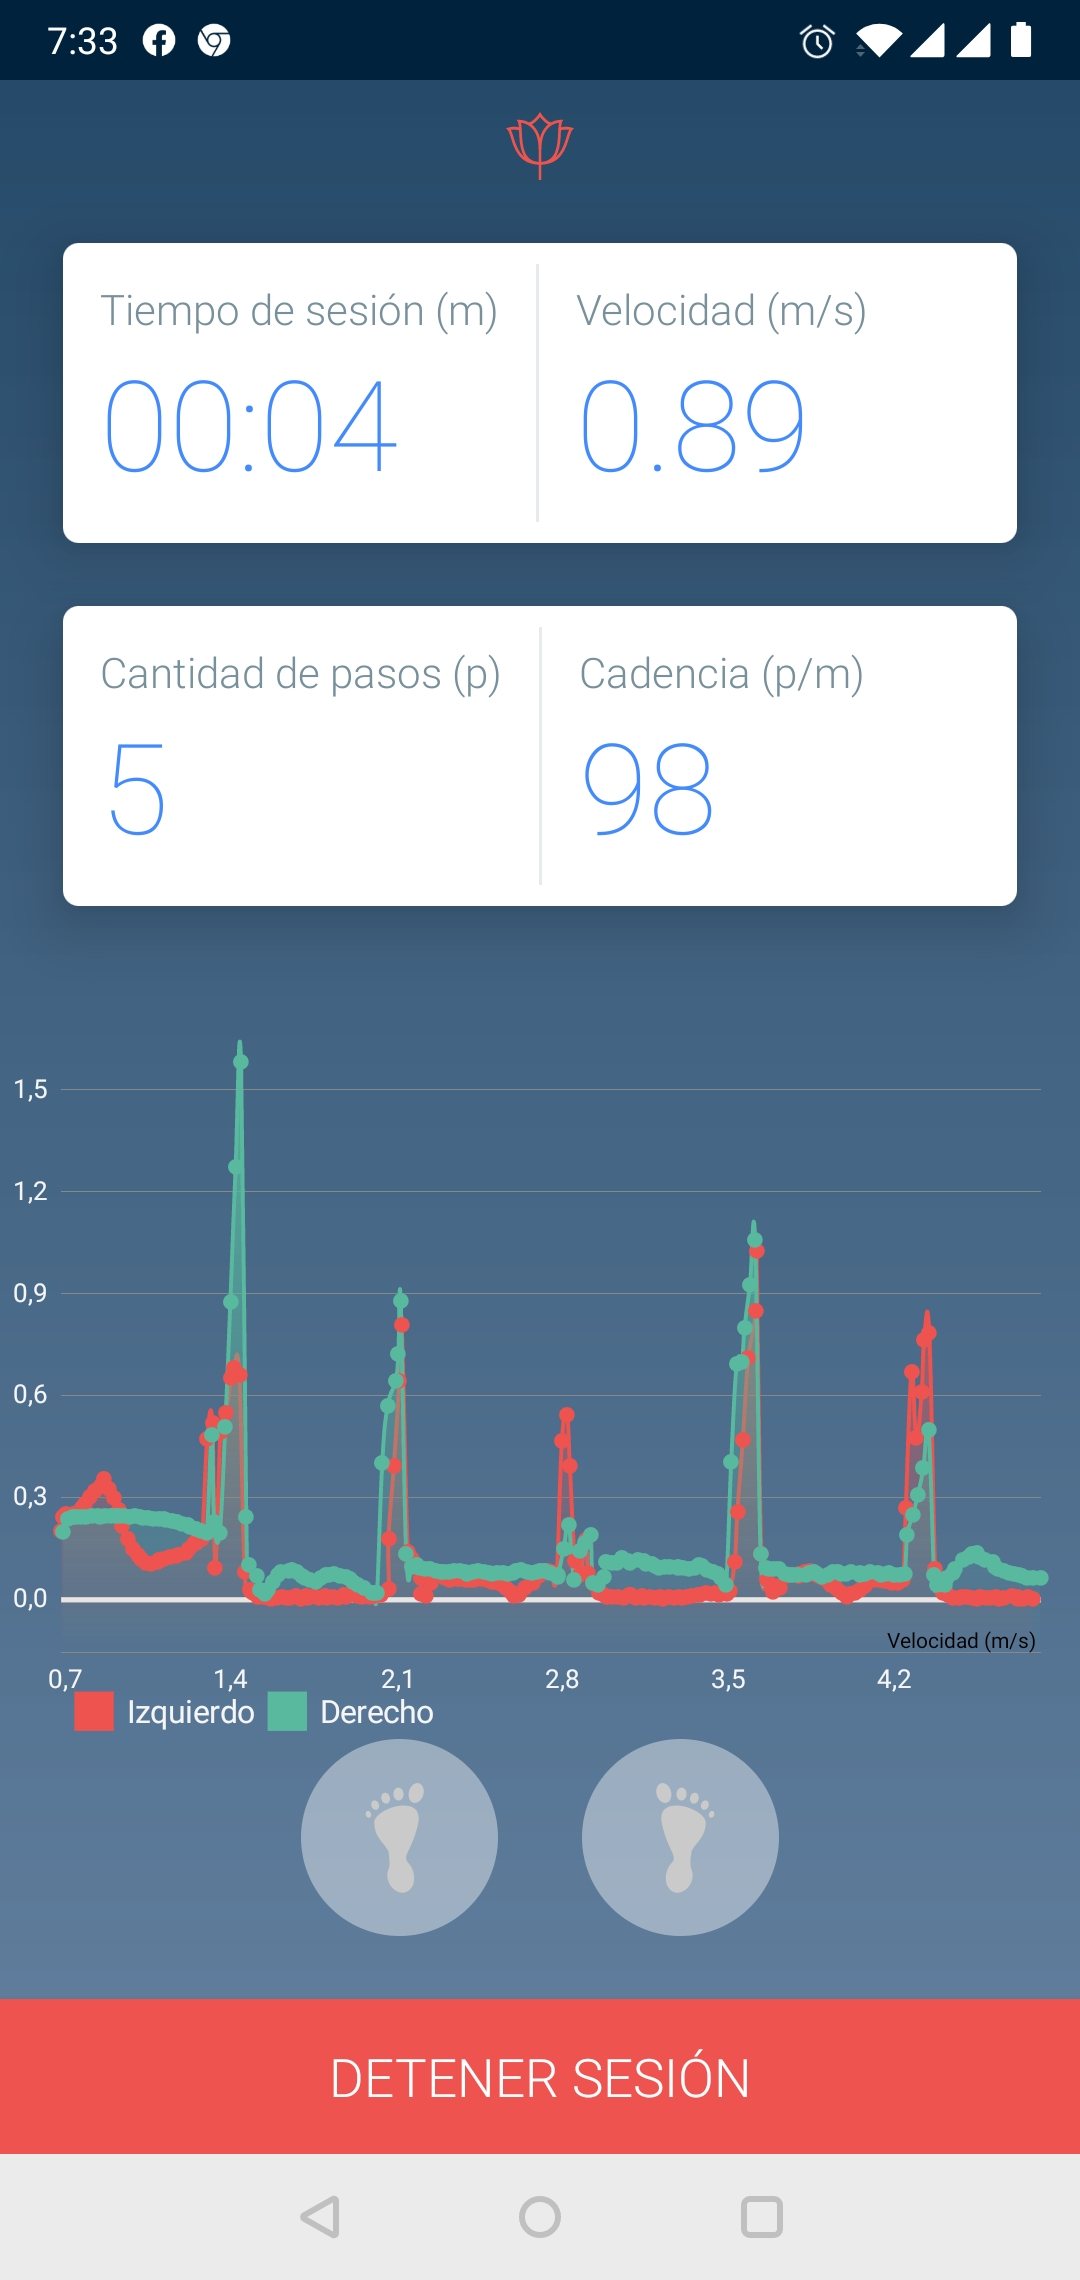
\includegraphics[height=9cm]{TESIS/imagenes/chap05/activity-active-session.JPG}
 \caption{Pantalla de una Sesión Activa PARKIBIP. El sistema reacciona en tiempo real a la marcha del paciente en rehabilitación. Dispara estímulos externos -vibración y/o sonido- y computa los parámetros espacio-temporales.}
 \label{fig:activity-active-session}
\end{figure}

Si bien las posibilidades son infinitas (i.e. debido a múltiples combinaciones de parámetros espacio-temporales), a continuación se detallan las principales reglas implementadas en PARKIBIP para decidir en qué momentos se producen dichos estímulos:

\begin{itemize}
    \item \textbf{On Heel Strike}: Cada vez que se produce un Heel Strike. Esta es una regla básica pero sumamente importante, ya que el funcionamiento correcto de la misma indica que se identifican adecuadamente los pasos de la marcha.
    \item \textbf{On FoG}: Transcurrido un intervalo de tiempo pre-definido sin que ocurra un Heel Strike. Esta regla es útil para detectar un evento de FoG (Bloqueo de la marcha), y a través del estímulo buscar interrumpirlo. 
    \item \textbf{On Instant Velocity Threshold}: Al atravesar umbrales de velocidad instantánea. En este caso se le notifica al paciente a través de estímulos sobre la velocidad instantánea, que la misma es muy alta o muy baja y podría ocasionar, por ejemplo, una caída por mayor velocidad.  
    \item \textbf{On Average Velocity Threshold}: Al atravesar umbrales de velocidad promedio. En este caso se le notifica al paciente mediante estímulos que el ritmo es demasiado bajo o alto. 
    \item \textbf{On Dynamic Calculated Time}: Ocurre luego de cierto intervalo de tiempo calculado en forma dinámica a partir de una primera caminata de configuración. Por ejemplo, el paciente realiza una marcha inicial de 6 pasos, y en base a los datos recopilados se computa el tiempo promedio entre los mismos. Luego, el estímulo vibratorio y/o sonoro se realiza en un periodo constante definido por este tiempo calculado -simulando una terapia rítmica de rehabilitación-. Desde el punto de vista terapéutico, podría resultar que la caminata del paciente sea demasiado lenta o demasiado rápida, por lo que el tiempo promedio calculado a partir de su caminata inicial no sería un buen indicador para efectuar el estímulo. Sin embargo, podría ser de utilidad para evaluar al paciente en deambulación respecto al ritmo de marcha y su uniformidad. 
\end{itemize}

Muchas de las grandes oportunidades de mejora que presenta el sistema, para ser implementadas a futuro, resultan de mejorar este módulo, ya sea implementando nuevas reglas o incrementando la inteligencia del mismo para decidir en qué momentos estimular. Además, se podrían crear nuevos tipos de estímulos, como por ejemplo el habla en lenguaje natural.

\section{Caso de uso: Flujo automatizado de Sesión Activa PARKIBIP}
\label{section:session-flow}

En línea con los subprocesos desarrollados y mencionados con anterioridad, se propone el caso de uso de Sesión Activa, fundamental para lograr comprender el funcionamiento de fondo de PARKIBIP. De esta manera, se elaboró el diagrama Fig. \ref{FIG:use-case-session}, que modela el flujo de tareas e información mediante la notación estándar BPMN 2.0.

Como se puede apreciar en la figura, el modelo integra los distintos componentes (e.g. \textit{DeviceConnection}, \textit{DataAnalyzer}, \textit{Services}, \textit{Threads}, \textit{Queues}, entre otros) y algoritmos numéricos desarrollados (e.g. filtro de Orientación, filtro de kalman, ZVD); luego los combina conforme a proponer una sinergia de trabajo que aumente el rendimiento del sistema, minimice el retardo de transmisión de eventos (por ende, los estímulos) y mantenga las responsabilidades bien delineadas (i.e. bajo acoplamiento y alta cohesión entre componentes). 

Para una mayor claridad y comprensión, el diagrama sintetiza el flujo a un único dispositivo inercial (en PARKIBIP, \textit{DeviceConnection}), esto significa que, existirán tantos componentes \textit{DataAnalyzers} con sus correspondientes \textit{KalmanFilterThreads} como dispositivos IMU o \textit{DeviceConnection} operando.

\newpage

\begin{figure}[H]
    \vspace{-3.0cm}
    \hspace*{-2.0cm}%
    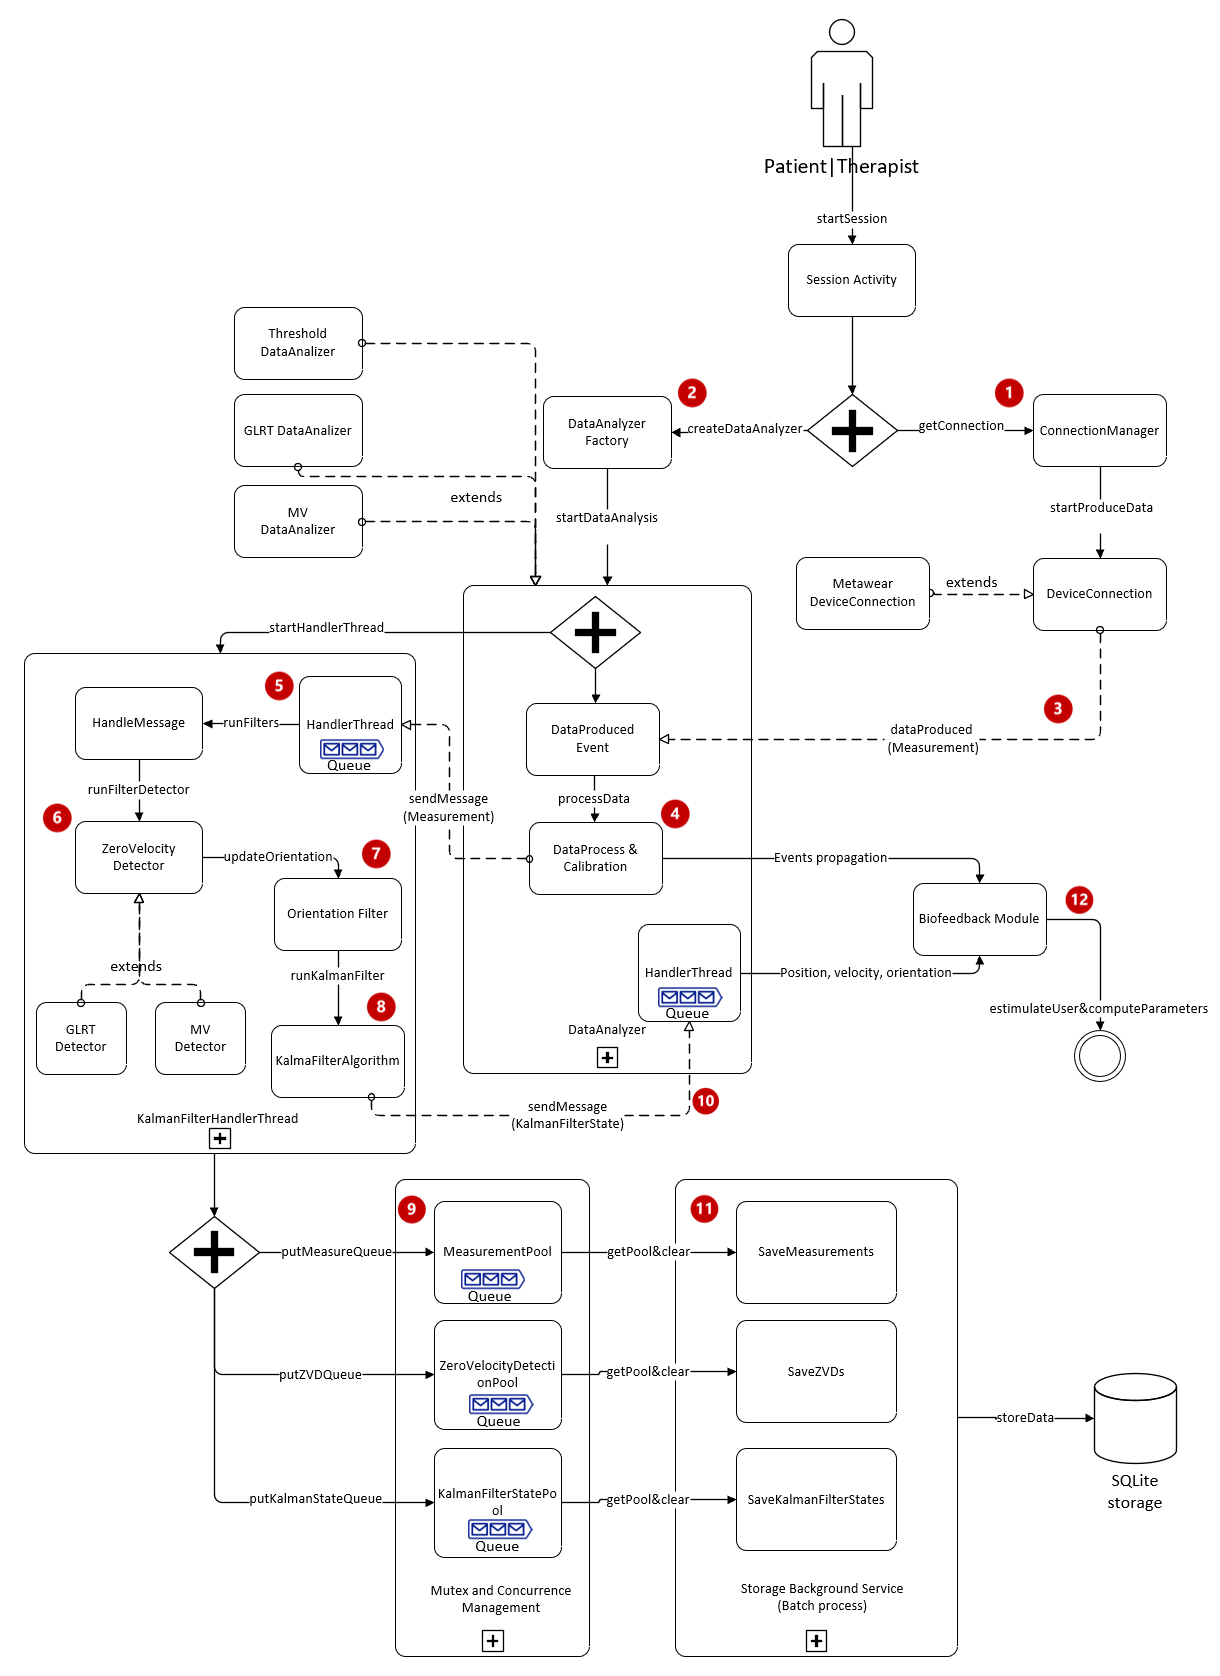
\includegraphics[clip,width=1.20 \columnwidth]{TESIS/imagenes/chap05/use-case-session.PNG}
    \caption{Flujo automatizado de Sesión Activa PARKIBIP. El modelo integra y combina los distintos componentes (e.g. \textit{DeviceConnection}, \textit{DataAnalyzer}, \textit{Services}, \textit{Threads}, \textit{Queues}, entre otros) y algoritmos numéricos que fueron desarrollados (e.g. filtro de Orientación, filtro de kalman, ZVD) con el fin de cumplir los objetivos del Proyecto. }
    \label{FIG:use-case-session}
\end{figure}

El Caso de Uso comienza cuando, un Terapeuta en una actividad de rehabilitación o un Paciente autónomo, inicia una Sesión previamente configurada en la aplicación PRKIBIP. En consecuencia, se disparan los eventos numerados en el diagrama Fig. \ref{FIG: ciclo}, y descriptos como notas al pie en lo que sigue:

\begin{enumerate}
    \item Mediante el manejador de conexiones -\textit{ConnectionManager}-, se obtiene la instancia lógica del dispositivo IMU particular a iniciar, un \textit{DeviceConnection} implementado por \textit{MetawearDevice}, cuya conexión fue previamente establecida. Luego de que se hayan establecido todas las configuraciones de los sensor y habilitado los productores de datos asíncronos, el sistema procede a iniciar la producción de datos de los distintos sensores. 
    \item De forma paralela, PARKIBIP crea un analizador de datos o \textit{DataAnalyzer} mediante la fábrica que encapsula dicha función -\textit{DataAnalyzerFactory}-. El tipo de \textit{DataAnalyzer} concreto a instanciar, dependerá de la selección vigente del mismo en el componente de configuraciones. Además, el sistema prepara e inicializa la recepción de eventos de datos de mediciones. En este punto, es importante resaltar que, el \textit{DataAnlyzer} será el responsable de orquestrar el procesamiento de la información a través de la delegación de tareas a ciertos módulos específicos.
    \item Cuando un sensor del IMU envía un evento de medición, éste es recibido mediante el componente \textit{DeviceConnection}; que analiza la secuencia de símbolos y la transforma a una estructura legible en la aplicación -modelo \textit{MeasurementModel}-. Luego, realiza un procesamiento previo del modelo de medición, ajustando las unidades al sistema internacional correspondiente y estandarizando la información.  Finalmente, dispara un evento de producción de datos a su \textit{DataAnalyzer} asociado.
    \item Recibido un evento de medición en el \textit{DataAnalyzer}, éste procede a ejecutar el flujo de procesamiento. En caso de que se requiera  calibrar la orientación del dispositivo IMU, el sistema realiza el el proceso de Calibración y descarta la medición. En otro caso, envía un evento de medición al manejador o \textit{Handler} del componente \textit{KalmanFilterHandlerThread}, así como también procesa la medición según el \textit{DataAnalyzer} concreto elegido. El resultado del procesamiento se propaga como evento al módulo de \textit{Biofeedback} de la aplicación.
    \item Primero, es crucial comprender el comportamiento de \textit{KalmanFilterHandlerThread}. Un Thread, representa un hilo de ejecución independiente al hilo principal de una aplicación; mientras que un \textit{HandlerThread} -en Android-, es una extensión del Thread que integra el concepto de \textit{Looper} y de \textit{Handler}. Un \textit{Looper} dentro de un Thread, tiene la capacidad de administrar adecuadamente los múltiples mensajes recibidos mediante su manejador -\textit{Handler}- y su estructura de almacenamiento del tipo Cola FIFO (del inglés, Queue). Entonces, el evento de medición recepcionado por el \textit{Handler} de \textit{KalmanFilterHandlerThread}, es inicialmente puesto en la Cola del \textit{Looper}, y luego atendido por el método \textit{HandleMessage}.
    \item La función \textit{HandleMessage}, responsable del procesamiento del filtro de Kalman, comienza ejecutando el detector de cero velocidad -\textit{ZeroVelociyDetector}-, dato requerido como parámetro por Kalman. El ZVD  concreto a emplear (e.g. GLRT, MV), se obtiene de la configuración actual del sistema.
    \item Luego, es vital la actualización de la orientación con cada medición entrante, no solo por
    ser pre-condición del algoritmo de Kalman, sino también para minimizar errores en la predicción de los parámetros espacio-temporales futuros. Por consiguiente, se corre el filtro de Orientación propuesto por S.Madwick en \cite{Madgwick}.
    \item Junto a la medición recopilada y los parámetros orientación y momento de velocidad cero -\textit{z\_value}-, el sistema ejecuta el filtro de Kalman. Este método es iterativo a medida que su función de actualización es invocada, y arroja como resultado un vector de estados con las estimaciones: posición, velocidad y orientación. Además, con el parámetro \textit{z\_value}, el algoritmo compensa/corrige las estimaciones según si el IMU se encuentra estacionario.
    Finalmente, el \textit{HandlerThread} de \textit{KalmanFilter} dispara un evento de mensajes hacia el \textit{Handler} del \textit{DataAnalyzer}, encapsulando el vector de estados resultante del procesamiento. A su vez, en paralelo, envía el modelo de medición y los resultados de cada algoritmo numérico -\textit{z\_value}, vector de kalman- a sus respectivos conjuntos de datos (en inglés, Data Pool).
    \item Cada unidad de \textit{Data Pool}, gestiona el acceso concurrente mediante la mutua exclusión de sus estructuras y recursos (e.g. Colas de mensajes). Los datos son puestos en el pool desde el hilo de ejecución Kalman, y recuperados en batch por un servicio de sistema de fondo.
    \item Análogo al punto 5, el mensaje con el vector de estados es recibido por el \textit{Handler} del \textit{DataAnalyzer} y puesto en la Cola del \textit{Looper}. En esta ocasión, el \textit{DataAnalyzer} actúa como pasamanos de información, propagando el estado hacia el modulo de \textit{Biofeedback}.
    \item Un servicio en Android, es un componente de una aplicación que puede realizar operaciones de larga ejecución en segundo plano. En PARKIBIP, cumple la responsabilidad del almacenamiento de datos en la base de datos SQL de la aplicación móvil. Con una frecuencia configurable y repetitiva, el servicio obtiene los datos a almacenar desde los Pooles de datos -en batch-, los vacía, y luego almacena los elementos en la base de datos.
    \item Concluyendo el proceso, el módulo de \textit{Biofeedback}, responsable de disparar los eventos de estimulación al Paciente, ejecuta las reglas clínicas apropiadas.
\end{enumerate}

\section{Administración de Identidades}

El sistema PARKIBIP fue diseñado específicamente para administrar dos niveles de usuarios, el Terapeuta y el Paciente en rehabilitación. En consecuencia, resulta imprescindible contar con un módulo particular, responsable de gestionar todas las funcionalidades requeridas para llevar adelante la gestión de identidades, proveer seguridad, y especialmente preservar la privacidad del Paciente. 

Así, en el presente apartado, se cubren detalles de la solución en cuanto a la administración de identidades, los protocolos que se deben usar y el flujo de autenticación requerido.

PARKIBIP decidió utilizar Auth0 \cite{Auth0}, como su proveedor de identidad como servicio (Identity as a Service, IDaaS, por sus siglas en inglés). Un IDaaS es un servicio basado en la nube para la gestión de identidades y accesos, a menudo también incluyen el inicio de sesión único (en inglés Single Sign-on, SSO), identidad federada, administración de contraseñas, entre otros. El razonamiento detrás de esta decisión fue la de integrar un servicio de terceras partes dedicado en la materia, y no implementar/mantener todos los aspectos complejos relativos a la seguridad, requeridos en ambientes productivos para datos sensibles. También, fue considerado y preparado en el diseño de la solución, la posibilidad de reemplazar fácilmente el módulo IDaaS por un nuevo micro-servicio (e.g. Agesic). Auth0 es una solución flexible y sencilla para agregar servicios de autenticación y autorización a las aplicaciones. De esta manera, el equipo y la organización pueden evitar el costo, el tiempo y el riesgo que conlleva la creación de su propia solución para autenticar, autorizar, discriminar y obtener información de los usuarios.

En definitiva, la aplicación Android PARKIBIP fue integrada a el proveedor de IDaaS Auth0 mediante el SDK del segundo, desarrollada en el lenguaje JAVA para Android y diseñada según la figura Fig. \ref{fig:activity-login}. 

\begin{figure}[H]
 \centering
 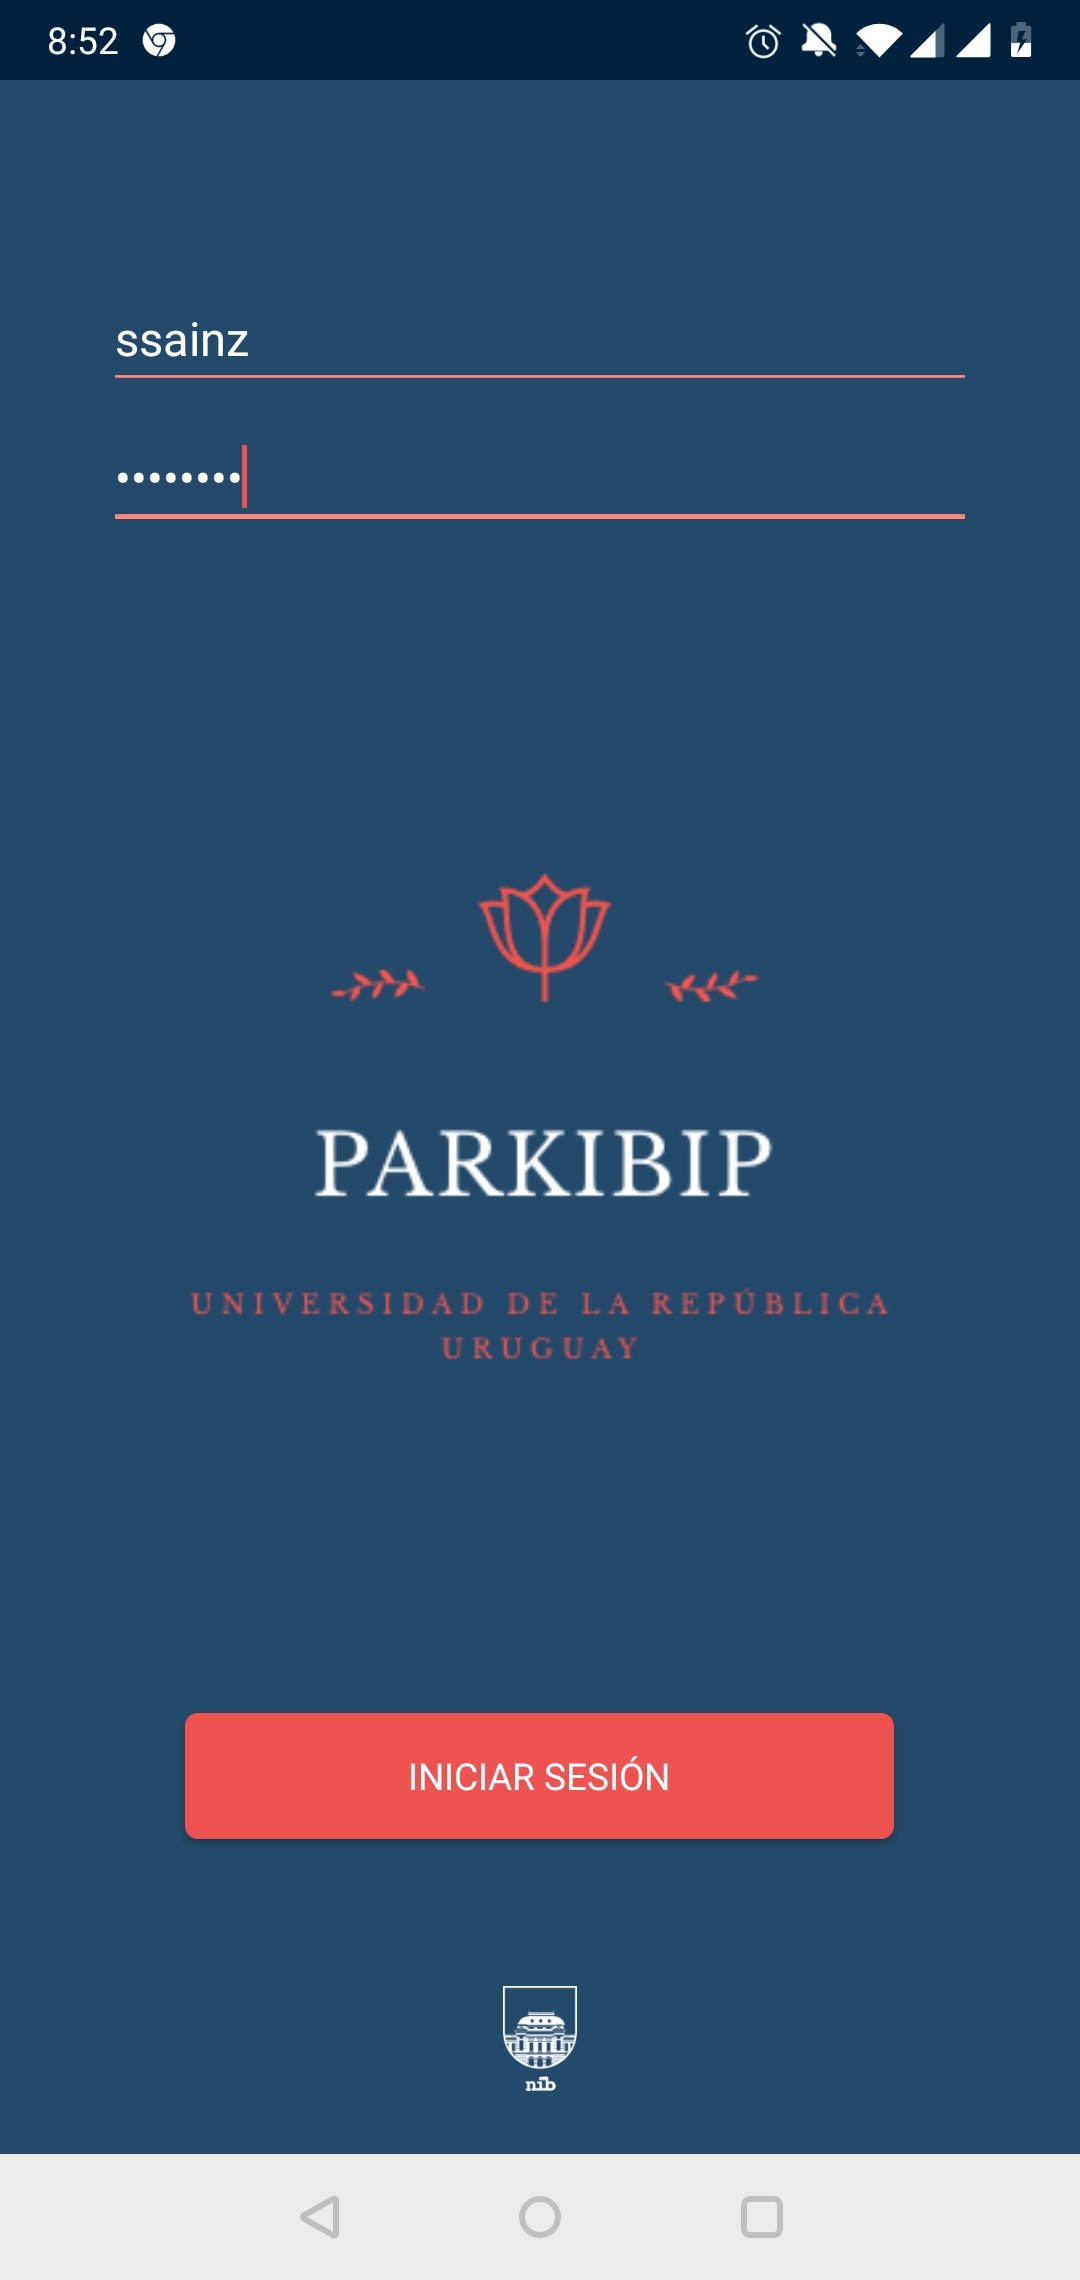
\includegraphics[height=8cm]{TESIS/imagenes/chap05/activity-login.JPG}
 \caption{Proceso de autenticación y autorización del Usuario. Se requieren los campos nombre de usuario y contraseña.}
 \label{fig:activity-login}
\end{figure}

En términos generales, para efectuar esta tarea se realizaron las configuraciones:

\begin{enumerate}
    \item Primero, fue creado un Auth0 tenant. Aquí es donde se configura el uso de Auth0, y donde los activos y recursos, como aplicaciones, conexiones y perfiles de usuario, se definen, administran y almacenan.
    \item Luego, se registró una aplicación nativa o móvil (en inglés, Native/Mobile App) que indica el tipo de aplicación que empleará los servicios en el \textit{Dashboard} de Auth0. Registrado el nuevo cliente, se obtuvo un ID de cliente único, necesario para efectuar llamados a las distintas funciones de la API de Auth0. Otro dato crucial, es el secreto del cliente (del inglés, Client Secret), análogo a una contraseña de aplicación que debe mantenerse confidencial en todo momento.
    \item Además, fue configurada la conexión que indica cómo los usuarios de PARKIBIP iniciarán sesión. Para ello, se uso la base de datos en la nube de Auth0.
    \item Finalmente, se implementaron las llamadas Reglas (Rules, en inglés). Estas, son funciones escritas en los lenguajes de programación JavaScript o C\#, ejecutadas en el mismo servidor de Auth0 justo después de una autenticación exitosa y antes de que el control regrese a la aplicación que realizo la invocación. Por ejemplo, fueron usadas para adjuntar en el Token información codificada del usuario.
\end{enumerate}

Otro aspecto importante, fue la manipulación del protocolo estándar abierto (RFC 7519) \textit{JSON Web Token} (JWT). El token JWT define una forma compacta y autónoma de transmitir información de forma segura entre las partes involucradas en el intercambio, como un objeto JSON. Dicha información puede ser verificada y confiada, ya que la misma está firmada digitalmente. Los JWT se pueden firmar usando el \textit{Client Secret} con el algoritmo de cifrado HMAC, o mediante el par de claves pública/privada empleando los algoritmos criptográficos RSA o ECDSA. En PARKIBIP se empleó el cifrado RS256 como algoritmo de firma digital para los \textit{JsonWebTokens}, en donde se firmará con la clave de firma privada y se puede verificar utilizando la clave de firma pública. Emplear JWT presenta variadas ventajas en comparación con los tokens web simples, y es usado con los siguientes objetivos:

\begin{itemize}
    \item Autenticación: cuando un usuario inicia sesión con éxito mediante sus credenciales, se devuelve un token de identificación -\textit{id\_token}- del tipo JWT.
    \item Autorización: una vez que un usuario ha iniciado sesión correctamente, PARKIBIP solicita acceso a rutas, servicios o recursos (por ejemplo, API) en nombre de ese usuario. Para hacerlo, en cada solicitud, debe pasar un Token de acceso -\textit{access\_token}-.
    \item Intercambio de información: Los JWT son una buena forma de transmitir información de forma segura entre las partes -firma digital-. 
\end{itemize} 

La figura Fig. \ref{FIG:payload-token} presenta un ejemplo de carga útil (del inglés Payload) encapsulada en el \textit{id\_token} durante el intercambio de información. Se aprecian metadatos del usuario, información descriptiva y transaccional del mismo. Valga como ejemplo el nombre, email, rol o tipo de usuario en el sistema, fecha de alta, entre otros. Por ende, el módulo de identidad de PARKIBIP, se encarga de interpretar el JSON conforme a acceder a los atributos de interés.

\begin{figure}[h!]
\centering
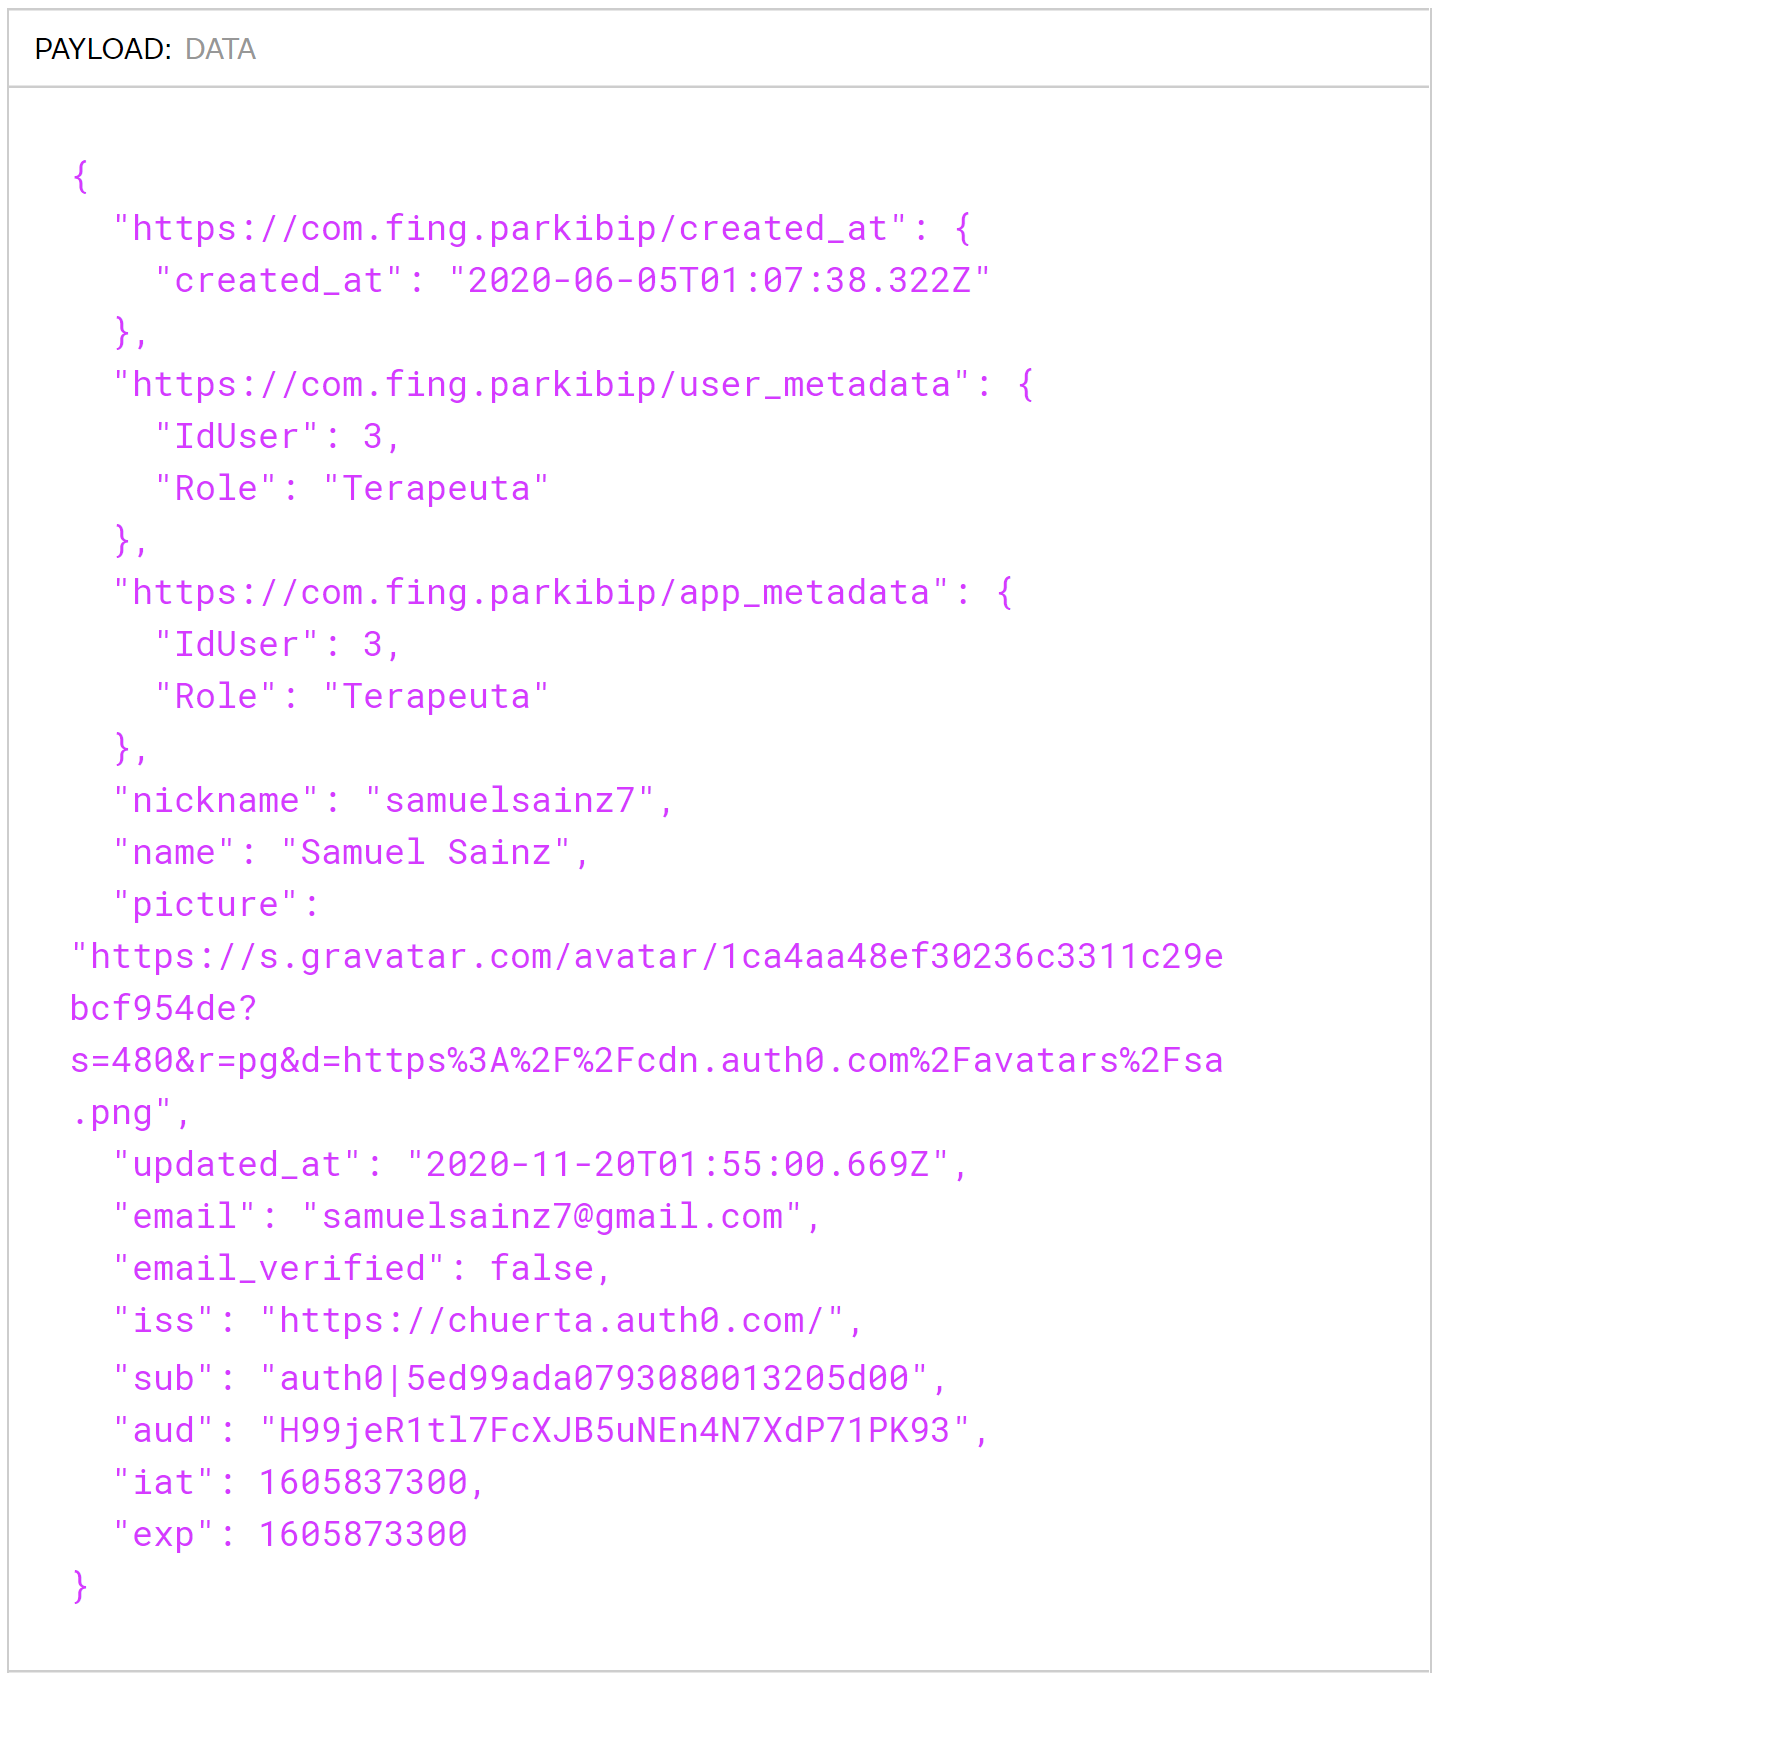
\includegraphics[width=\textwidth]{TESIS/imagenes/chap05/payload-token.PNG}
\caption{Ejemplo de carga útil (del inglés Payload) durante el intercambio de información embebida en el token de identificación. Se aprecian metadatos del usuario, información descriptiva y transaccional (e.g. nombre, email, rol o tipo de usuario en el sistema, etc.)}
\label{FIG:payload-token}
\end{figure}

Asimismo, mediante el decodificador, se puede apreciar el algoritmo criptográfico empleado y el tipo de token generado. Véase la figura Fig. \ref{FIG:header-token}.

\begin{figure}[H]
\centering
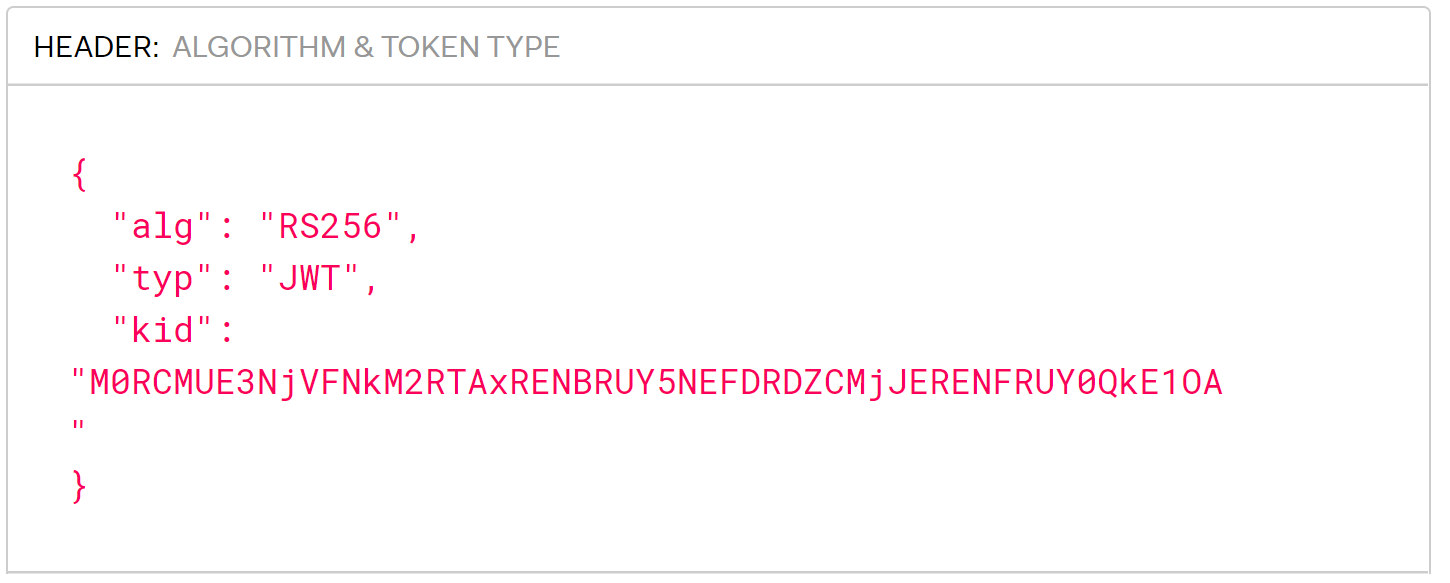
\includegraphics[width=\textwidth]{TESIS/imagenes/chap05/header-token.PNG}
\caption{Ejemplo de encabezado de un token JWT. Especifica el algoritmo de cifrado y el tipo de token generado.}
\label{FIG:header-token}
\end{figure}

A continuación, se mencionan otras tareas de desarrollo relativas al módulo de identidad:
\begin{itemize}
    \item Inclusión de la SDK de Auth0 mediante la dependencia \textit{'com.auth0.android:auth0:1.+'}. La librería encapsula la comunicación con las API de autenticación y administración de Auth0.
    \item Administración de propiedades de acceso: \textit{com\_auth0\_domain}, \textit{com\_auth0\_client\_id}.
    \item \textit{Callback}: Un \textit{callback}, es una URL en la aplicación en donde Auth0 redirige al usuario después de que el mismo se ha autenticado.
    \item \textit{Logout URL}: Una URL de cierre de sesión, es una URL en la aplicación a la que Auth0 puede retornar luego de que el usuario haya cerrado la sesión del servidor de autorización. En PARKIBIP se definió: \textit{fing://parkibip.auth0.com/android/parkibipapp/callback}.
    \item Función Login: Método responsable de realizar el flujo de autenticación y distinción por niveles de usuario (Terapeuta, Paciente).
    \item Función Logout: Método encargado de administrar el cierre de la sesión activa en la aplicación.
    \item Administración de credenciales: Componente responsable de administrar los tipos de tokens de Auth0, por ejemplo, token para actualización -\textit{refresh\_token}-, token de identidad -\textit{id\_token}-, token de acceso -\textit{access\_token}-.
\end{itemize}

El flujo de autenticación empleado a través de Auth0, se basa en \textit{OAuth 2.0}, utilizando una clave de prueba para intercambio de código (del inglés, Proof Key for Code Exchange, conocido por PKCE) La ilustración Fig. \ref{FIG:flow-PKCE}, tomada de \cite{Auth0:PKCE} y adaptada al proyecto, refleja el flujo de intercambios de mensajes durante el proceso de autenticación que efectúa PARKIBIP. 

\begin{figure}[!h]
\resizebox{\textwidth}{!}{
\centering
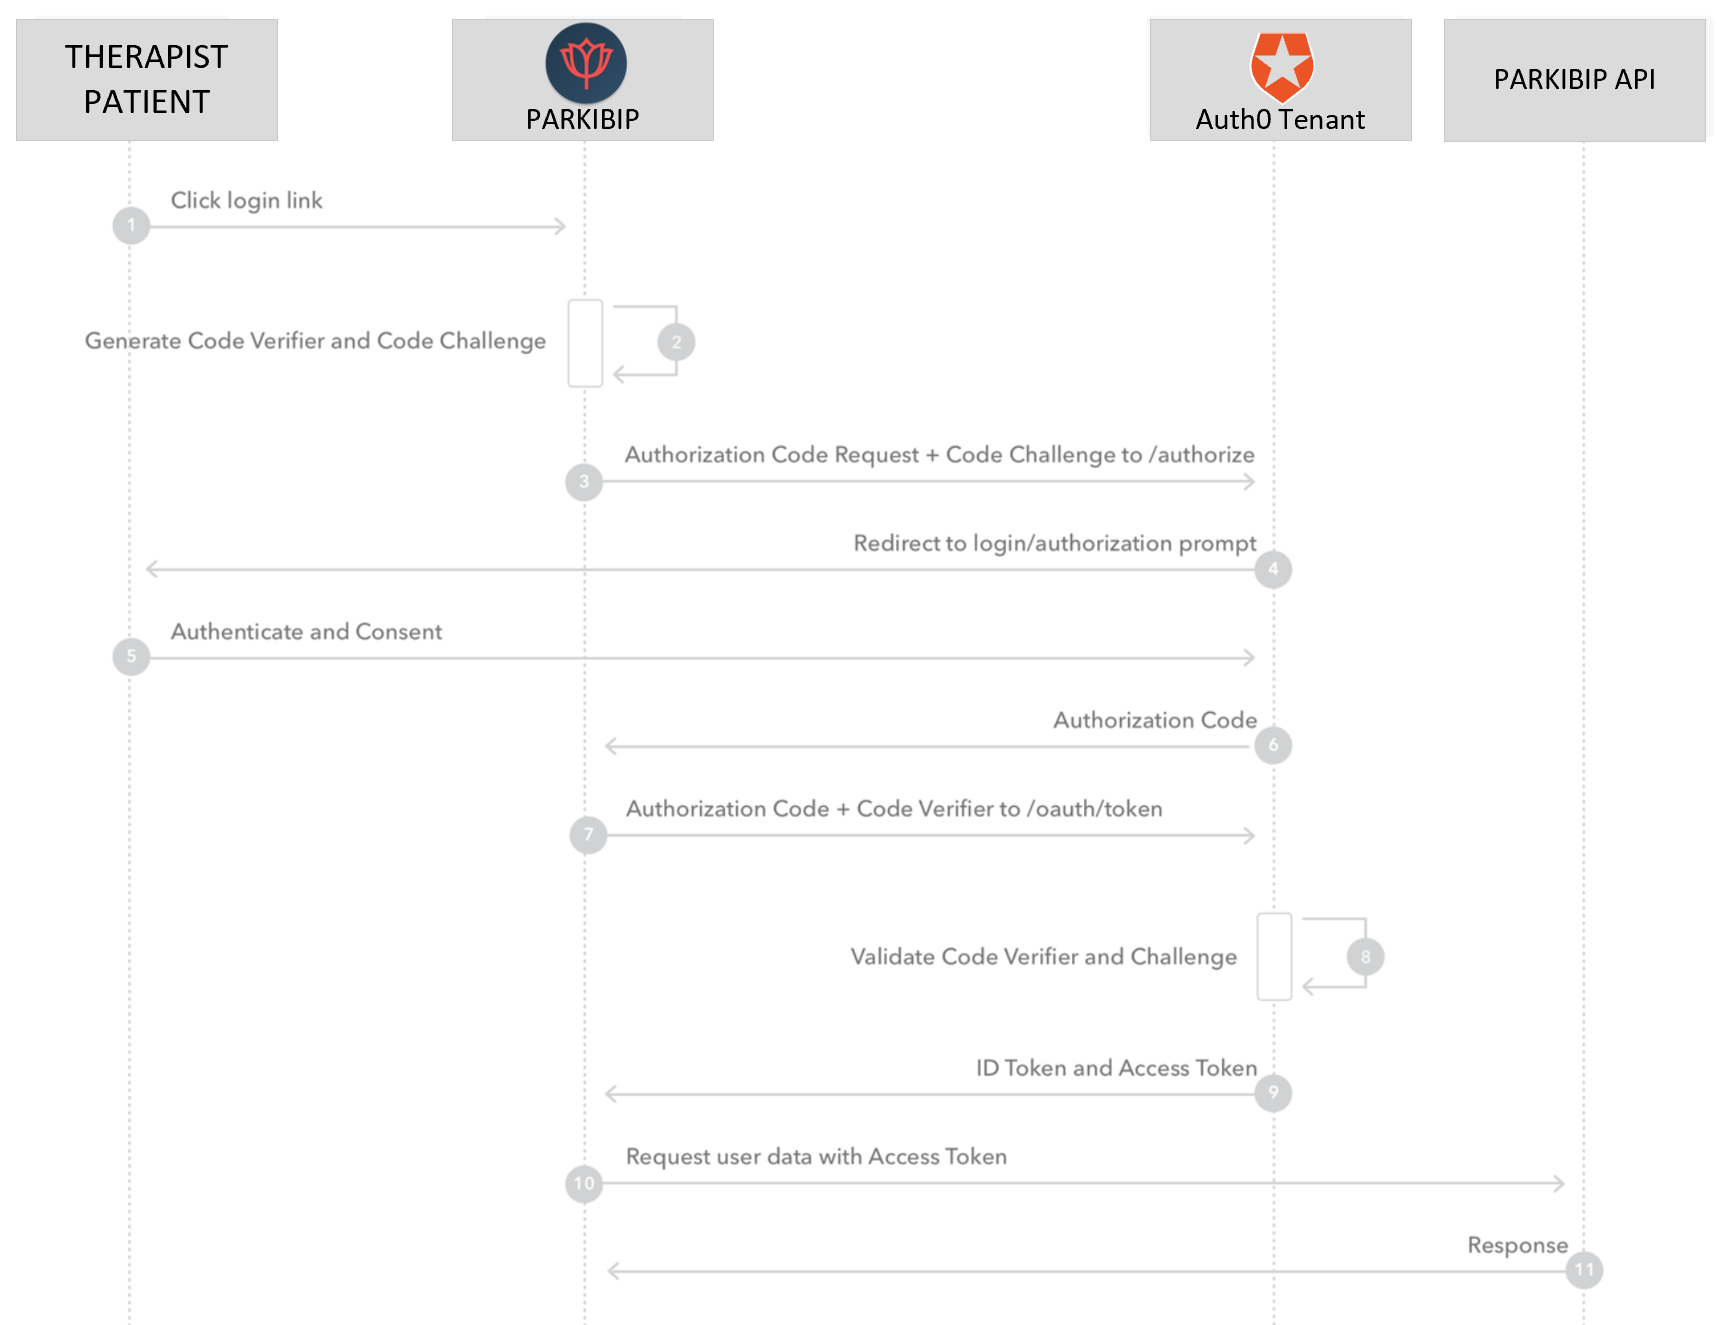
\includegraphics{TESIS/imagenes/chap05/parkibip-auth0-flow.PNG}}
\caption{Flujo de autenticación y autorización entre PARKIBIP y Auth0 Tenant, a través del protocolo clave de prueba para intercambio de código (PKCE). Cita a \cite{Auth0:PKCE} y adaptación a PARKIBIP}
\label{FIG:flow-PKCE}
\end{figure}

En resumen, el procedimiento de autenticación e implícito al usuario sigue el proceso:
\begin{enumerate}
    \item El Paciente o Terapeuta intenta ingresar al sistema, para ello, hace click en Iniciar Sesión dentro de la aplicación.
    \item Mediante la invocación a la función LogIn de el SDK de Auth0, se crea un verificador de código -\textit{code\_verifier}- con cifrado aleatorio y a partir de ésto se genera un desafío de código -\textit{code\_challenge}-.
    \item El SDK en Android redirige al usuario al Servidor de autorización de Auth0 invocando el endpoint \textit{/authorize} de su API, adjuntando el \textit{code\_challenge}.
    \item El servidor de Auth0 redirige al usuario a la solicitud de inicio de sesión y autorización.
    \item Luego, el usuario se autentica utilizando una de las opciones de inicio de sesión pre-establecidas -usuario y contraseña-. En caso de ser el primer inicio de sesión, se despliega una página de consentimiento con los permisos que la aplicación le otorgará a Auth0.
    \item El servidor de autorización, almacena el \textit{code\_challenge}, luego, redirige al usuario a la aplicación con un código.
    \item El SDK envía el código recibido junto a el \textit{code\_verifier} -creado en el paso 2- al servidor de autorización de Auth0, endpoint \textit{/oauth/token}.
    \item El servidor de  autorización de Auth0 verifica los datos  \textit{code\_challenge} y \textit{code\_verifier} enviados.
    \item Finalmente, Auth0 responde con los tres tokens necesarios: \textit{id\_token}, \textit{access\_token}, \textit{refresh\_token}.
\end{enumerate}

Así, cada vez que un usuario intenta autenticarse, Auth0 verifica la identidad y envía la información requerida a PARKIBIP. Para concluir, la imagen Fig. \ref{FIG:idtoken}, brinda un ejemplo de token de identificación -\textit{id\_token}-, resultado de ejecuta el flujo de proceso autenticación y autorización.

\begin{figure}[!h]
\resizebox{\textwidth}{!}{
\centering
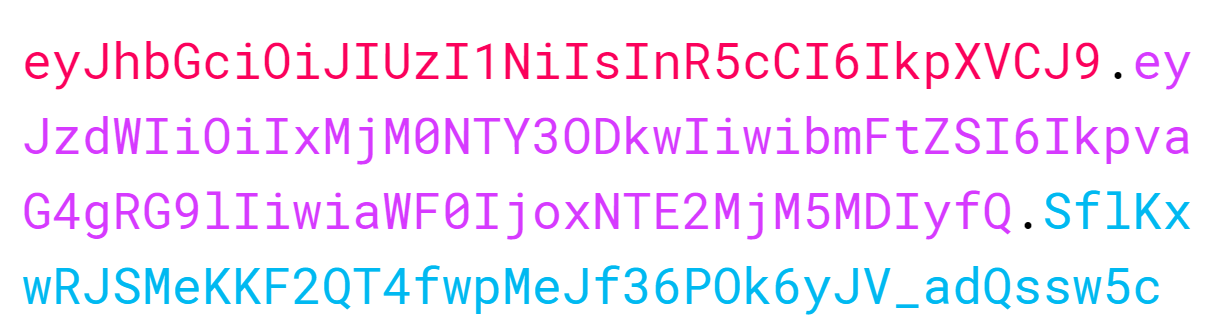
\includegraphics{TESIS/imagenes/chap05/token.PNG}}
\caption{Ejemplo de token de identidad --\textit{id\_token}-- con formato JWT, obtenido como resultado del flujo \ref{FIG:flow-PKCE} }
\label{FIG:idtoken}
\end{figure}

\section{Administración de Terapeutas y Pacientes}

PARKIBIP tiene como propósito la ejecución de sesiones de rehabilitación para un Paciente y coordinadas por un Terapeuta, por consiguiente es imprescindible la administración de Terapeutas y Pacientes. Es necesario llevar el registro de los mismos para asociar las diferentes sesiones de terapia. Mantener los datos de los pacientes, entre otras cosas, permitió el desarrollo de funcionalidades como ser la visualización del listado de los pacientes para un Terapeuta particular, ver sus sesiones, y luego medir el progreso de cada paciente. Dentro de las historias de usuario del sistema, se desea que, tanto los pacientes como los terapeutas, puedan observar la información vinculada a las distintas sesiones, mantener su registro y compararlas para analizar el progreso entre cada sesión. 

La figura Fig. \ref{FIG:users-and-sessions-class-diagram} presenta el diagrama de clases con el diseño de esta sección del sistema. La entidad \textit{User} -Usuario-, representa tanto a los pacientes como a los terapeutas y mantiene la información descriptiva de éstos, como lo es el nombre, el apellido y un identificador único auto-generado en el sistema. Luego, utilizando el concepto de herencia, se extiende la clase \textit{Patient} -Paciente- que además integra datos particulares que se desean conocer para éste nivel de usuario: edad, documento, observaciones relevantes (e.g. ``rigidez en pierna derecha'', ``episodios de FoG'' o cualquier tipo de observación sobre el paciente que sea relevante). Similar, se tiene una entidad \textit{Therapist} -Terapeuta- que hereda de \textit{User}, y además adjunta la información específica de un terapeuta, por ejemplo el centro médico en el cual trabaja. A su vez, \textit{UsersManager} es una componente que tiene el conocimiento para administrar los niveles de usuarios e identificar cuál es el paciente activo para las futuras sesiones. A través de \textit{UsersManager} se pueden obtener los distintos usuarios, agregar un nuevo paciente, recuperar un paciente particular a través de su identificador, etc. 

\begin{figure}[H]
    \hspace*{-2.0cm}%
    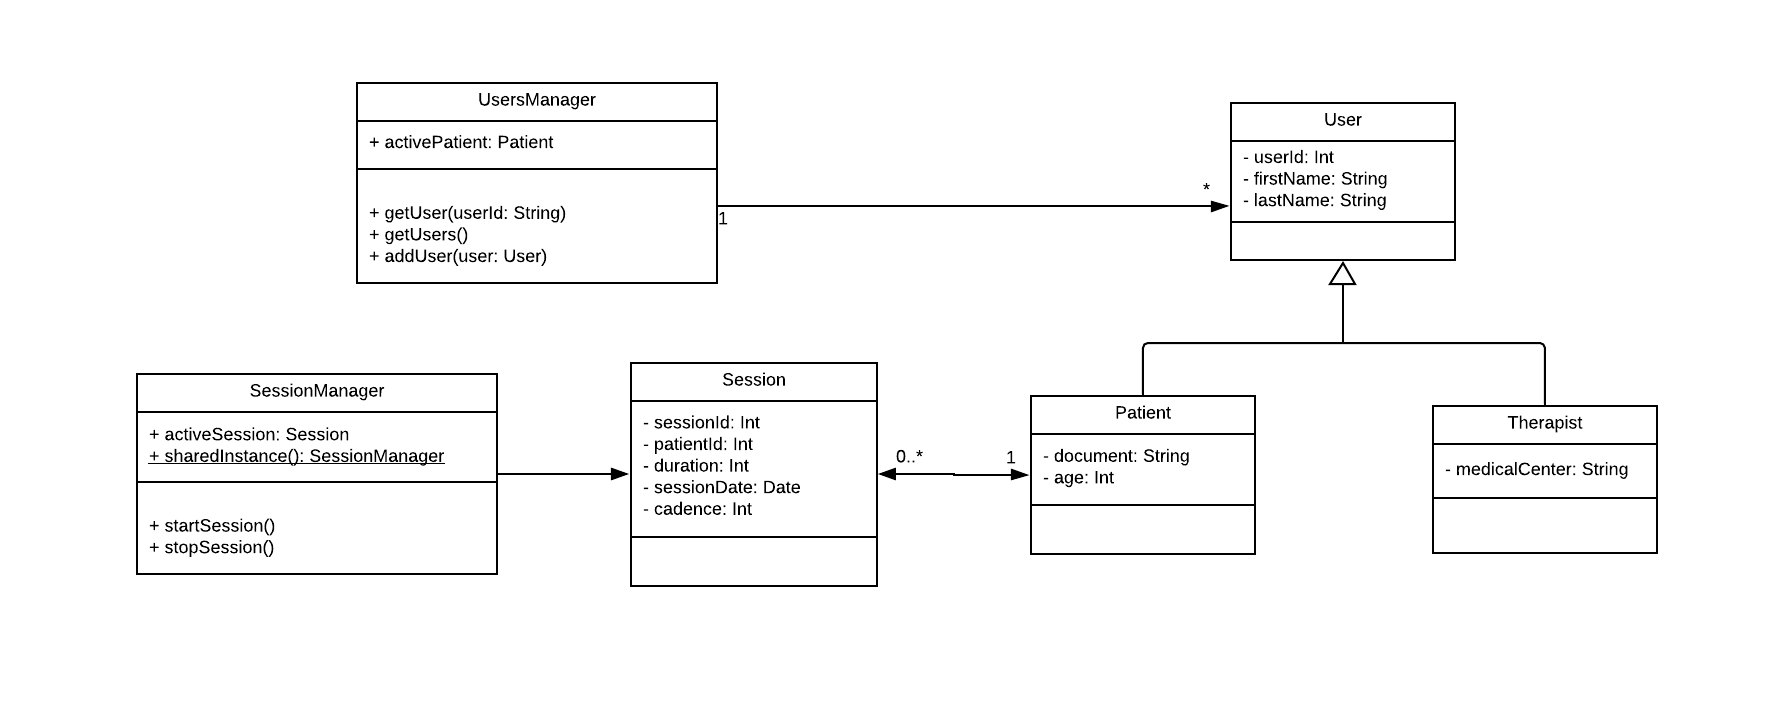
\includegraphics[clip,width=1.25 \columnwidth]{TESIS/imagenes/chap05/users-and-sessions-class-diagram.png}
    \caption{Diagrama de clases del módulo de la aplicación Android donde se representan los terapeutas, pacientes y las sesiones realizadas.}
    \label{FIG:users-and-sessions-class-diagram}
\end{figure} 

Dentro del menú de navegación de la aplicación, para visualizar el listado de pacientes almacenados, se puede consultar el acceso directo ``Perfiles''. La figura Fig. \ref{fig:activity-users}  muestra dicha pantalla. Con el fin de trabajar la amigabilidad del sistema, se le proporciona al usuario la capacidad de filtrar los pacientes utilizando la funcionalidad de búsqueda, accesible a través del icono de búsqueda en la barra superior de navegación de la pantalla. 

\newpage

\begin{figure}[H]
 \centering
 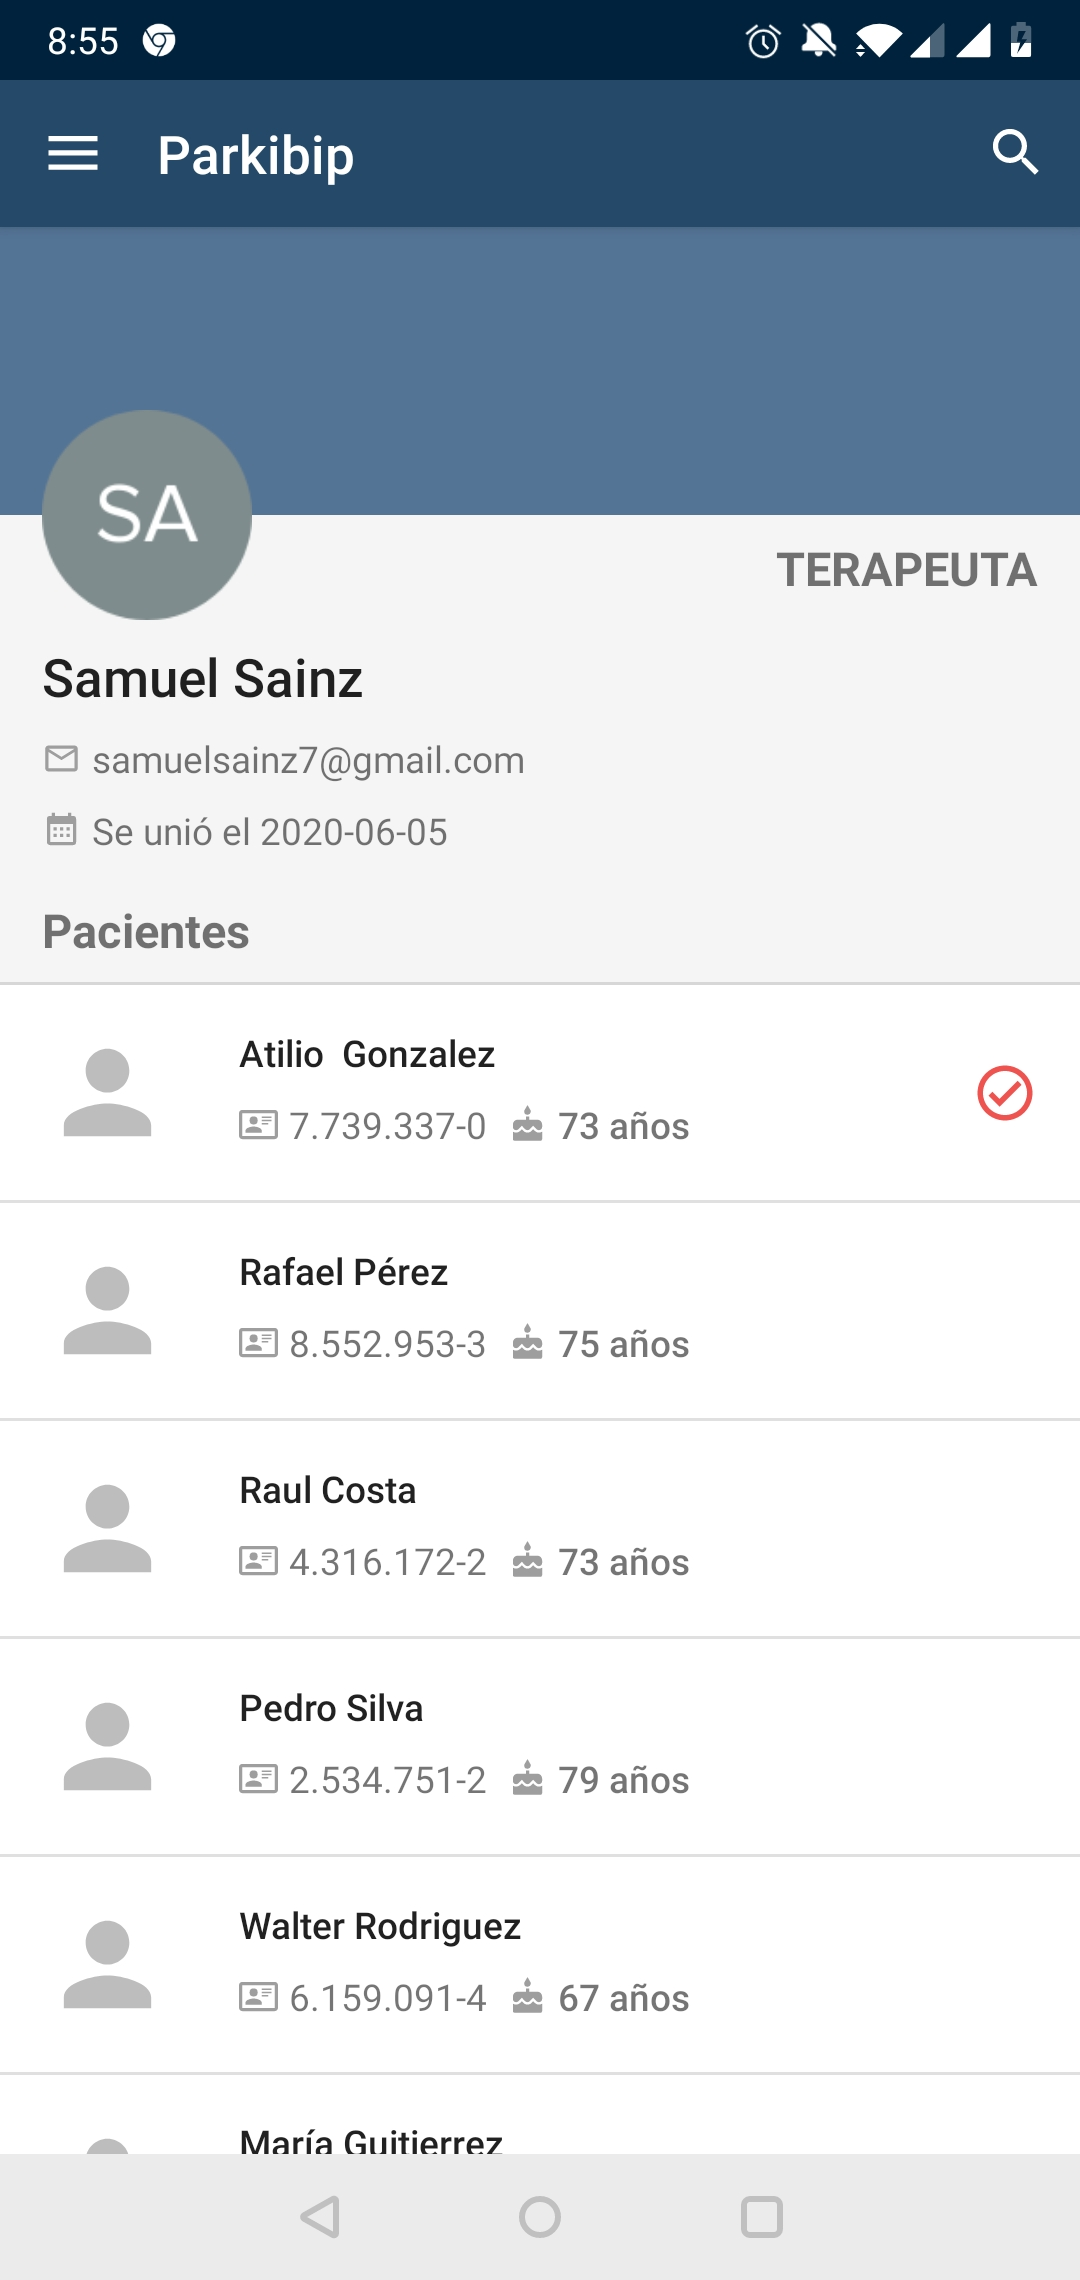
\includegraphics[height=8cm]{TESIS/imagenes/chap05/activity-users.JPG}
 \caption{Visualización de perfiles de usuarios. Funcionalidades: (i) Ver información descriptiva del usuario logueado, (ii) Ver el listado de pacientes -en caso de ser un terapeuta-, (iii) Seleccionar el paciente activo para futuras sesiones de rehabilitación.}
 \label{fig:activity-users}
\end{figure}

\section{Administración de Sesiones de rehabilitación}

PARKIBIP es un sistema rehabilitador en base a sesiones clínicas, por lo tanto, cada paciente tendrá tantas sesiones PARKIBIP -representadas con la clase \textit{Session}- como sesiones de rehabilitación. Para cada una de estas sesiones, se conoce el identificador del paciente que realizó la sesión, la fecha de realización, la duración, así como los parámetros espacio-temporales resultantes de su procesamiento: cadencia, cantidad de pasos, velocidad promedio, duración -ver figura Fig. \ref{fig:activity-summary}-.

\newpage

\begin{figure}[H]
 \centering
 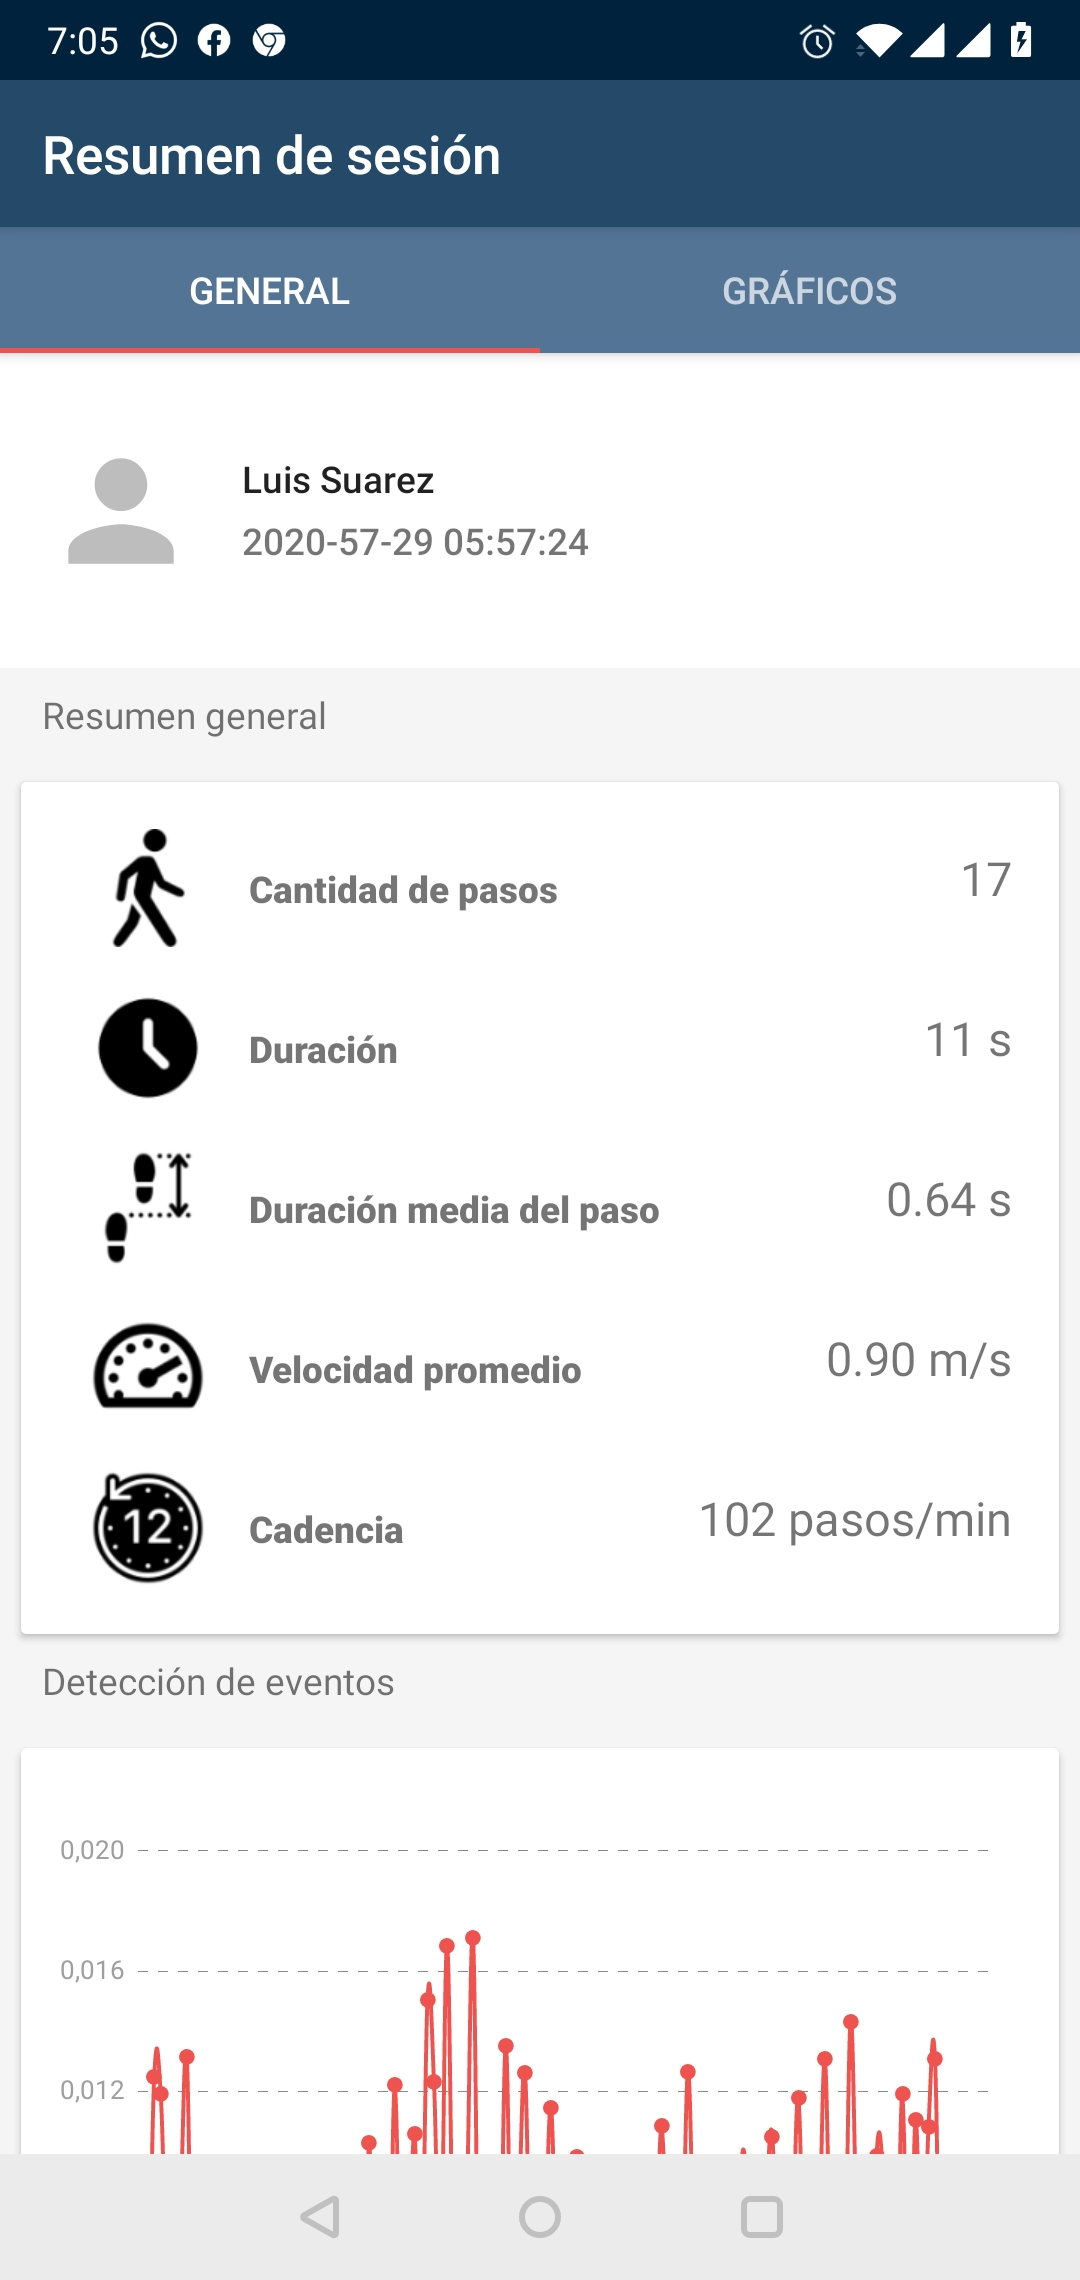
\includegraphics[height=8cm]{TESIS/imagenes/chap05/activity-session-summary.JPG}
 \caption{Resumen general y detallado de una sesión. Se presenta el comportamiento de la marcha en términos de valores de parámetros espacio-temporales y de forma gráfica.}
 \label{fig:activity-summary}
\end{figure}

Por su parte, el componente \textit{SessionsManager} es la clase encargada de administrar las sesiones realizadas, tiene la responsabilidad de crear, listar, remover sesiones, y sobretodo identificar una sesión viva. Durante una sesión PARKIBIP, es el \textit{SessionsManager} quien mantiene la instancia de sesión activa, útil para guardar en la sesión en la base de datos finalizada la sesión, combinarla con las mediciones y con los resultados del post-procesamiento. 

Una vez que la sesión es completada, se almacena en la base de datos el resumen genérico y detallado de la misma, generando una pantalla específica en la aplicación conforme a medir los resultados logrados. Además, dicha sesión se puede encontrar en el historial de sesiones de la aplicación, a través del menú de navegación de la aplicación, acceso ``Historial de sesiones''. La figura Fig. \ref{fig:activity-history-session} visualiza dicha pantalla. 

\newpage

\begin{figure}[H]
 \centering
 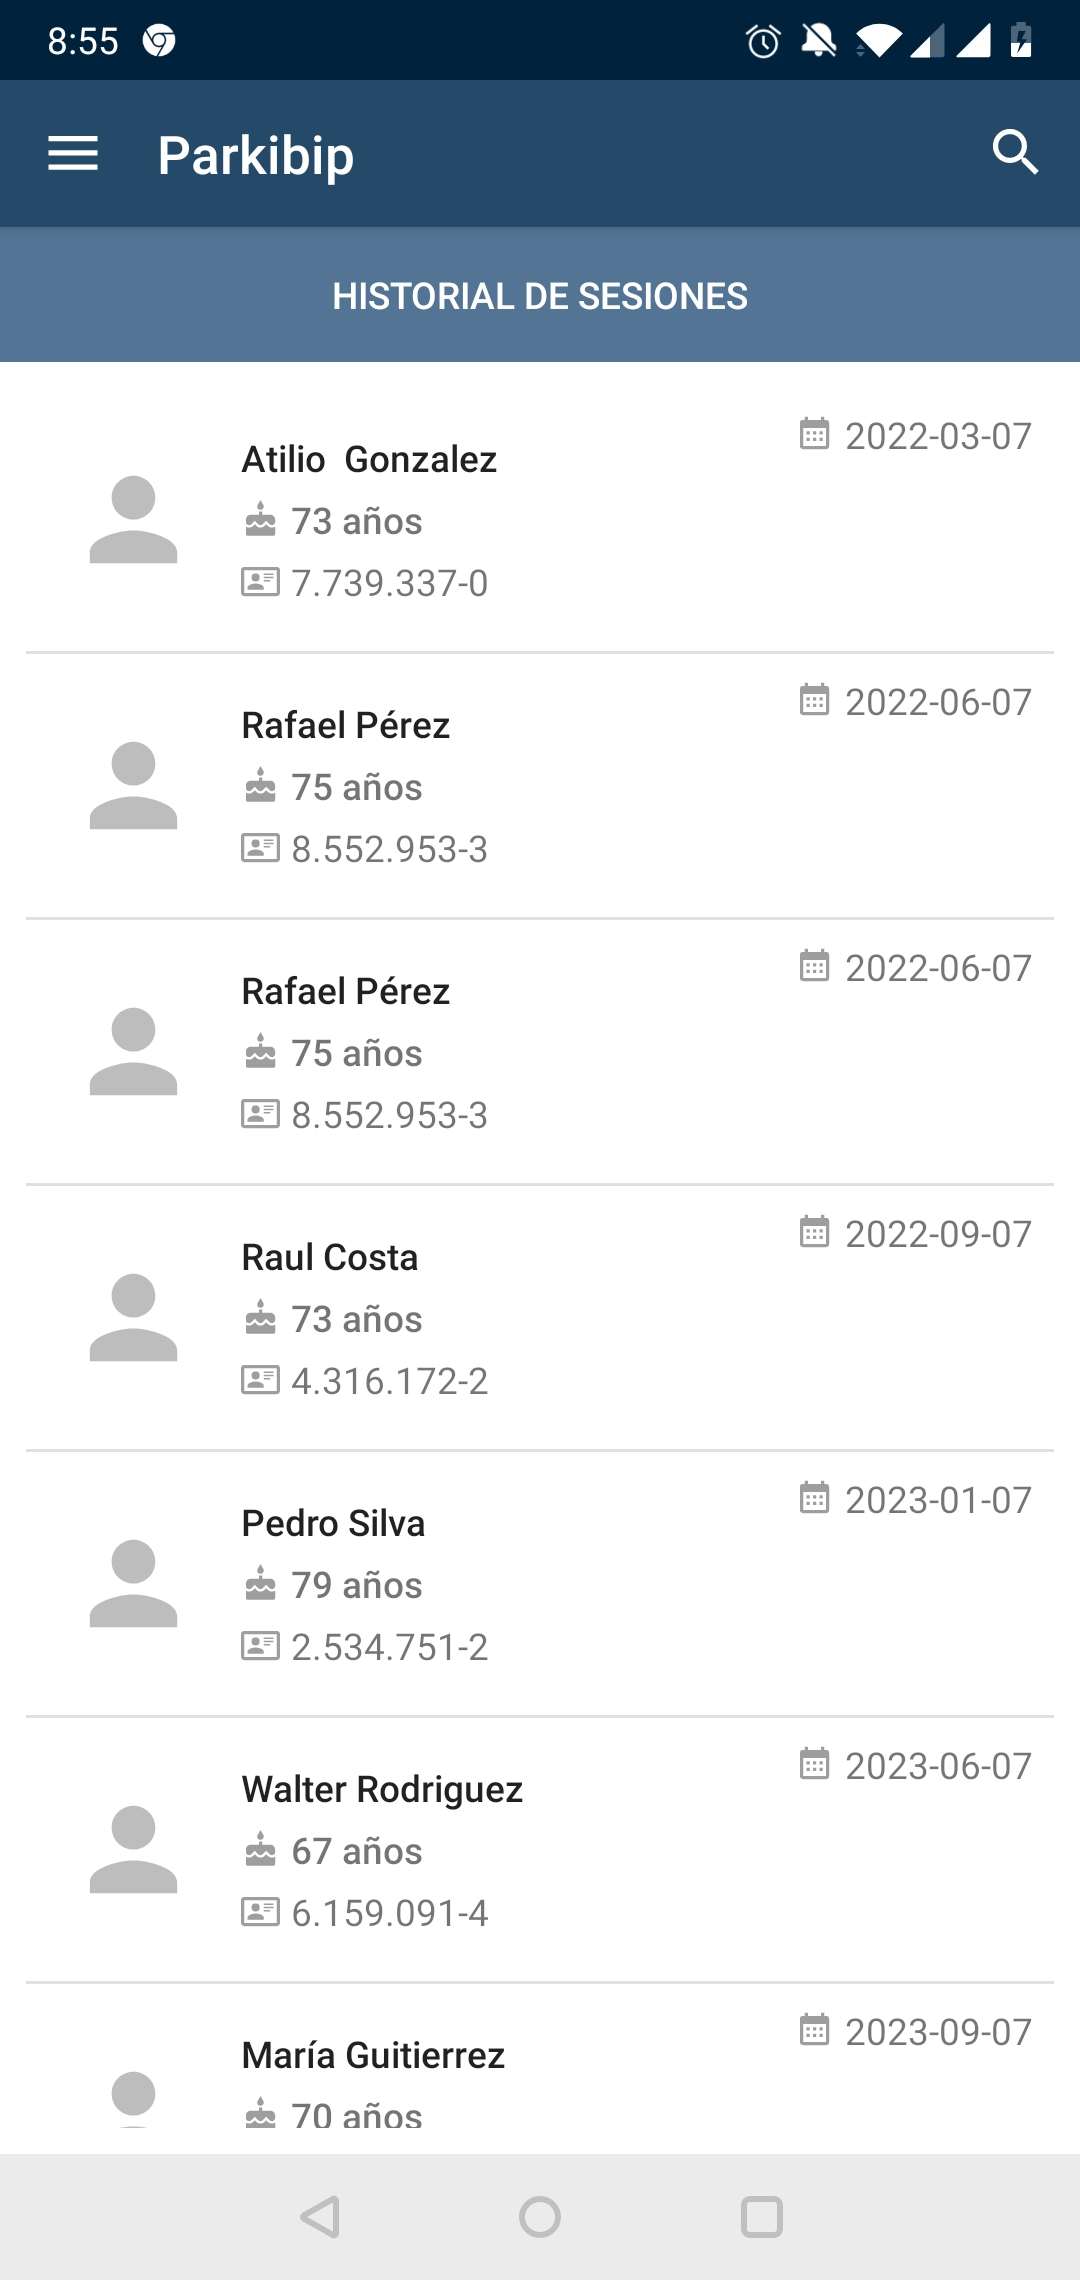
\includegraphics[height=8cm]{TESIS/imagenes/chap05/session-list.jpg}
 \caption{Historial de sesiones. Ordenadas cronológicamente con su correspondiente fecha de realización y paciente evaluado. Permite acceder a su resumen mediante su selección.}
 \label{fig:activity-history-session}
\end{figure}

Cada una de las sesiones listadas, presenta la información del paciente que realizó la sesión. Adicionalmente, el usuario puede filtrar las sesiones digitando el nombre del paciente en la barra de búsqueda situada en la parte superior de la pantalla. Respecto a las sesiones, también se conocen las mediciones y los resultados de los procesamientos realizados en el transcurso de toda la sesión. En la pantalla donde se resume la sesión, se pueden ver las gráficas detalladas en función del tiempo: velocidad, trayectoria y aceleración.


\section{Diagrama de clases}

El objetivo de esta sección es, presentar el diseño de la aplicación Android mediante un diagrama de clases simplificado, ilustrado en la figura Fig. \ref{FIG:class-diagram-design}. Si bien, por simplicidad, se omiten algunas entidades del sistema, en el siguiente diagrama se pueden ver los elementos fundamentales de la aplicación móvil. El diagrama brinda una visión general de cómo está diseñado el sistema, así como sus responsabilidades y la interacción entre ellos.

\newpage

\begin{figure}[H]
    \hspace*{-2.0cm}%
    \includegraphics[clip,width=1.25 \columnwidth]{TESIS/imagenes/chap05/Parkibip-Design.png}
    \caption{Diagrama de clases de la aplicación Android PARKIBIP. Se muestran en este diagrama los componentes esenciales del sistema y se omiten varios por simplicidad.}
    \label{FIG:class-diagram-design}
\end{figure}

Para diseñar PARKIBIP se tuvieron en cuenta varios principios de diseño que favorecen las cualidades del sistema como mantenibilidad, escalabilidad, calidad, entre otras. Como se puede ver en el diagrama, existe una alta cohesión de los componentes y un bajo acoplamiento entre éstos. Se intentó no repetir código, mantener responsabilidades únicas, abstraer comportamiento mediante interfaces y clases abstractas. En PARKIBIP se tuvieron en cuenta los principios de diseño SOLID. SOLID es un acrónimo que resume los cinco principios de diseño de diagramas de clases\cite{Chebanyuk2016}:

\begin{itemize}
    \item \textbf{S}ingle Responsibility: Responsabilidad única
    \item \textbf{O}pen-Closed: Abierto-Cerrado
    \item \textbf{L}iskov Substitution: Principio de Sustitución de Liskov
    \item \textbf{I}nterface Segregation: Principio de Segregación de Interfaces
    \item \textbf{D}ependency Inversion: Inversión de la Dependencia 
\end{itemize}

El principio de \textbf{responsabilidad única} es quizás el más simple de identificar observando el diagrama de clases, ya que es fácil notar que cada clase del sistema tiene una única función u objetivo. Para mencionar un ejemplo, se puede ver que \textit{ConfigurationProvider} es encargado de proveer las configuraciones, administrarlas, modificarlas, etc; pero la configuración en sí está dada por la clase \textit{Configuration}. \textit{DataAnalyzerFactory} es una clase que consulta a \textit{ConfigurationProvider} por una instncia de \textit{Configuration} para poder crear la instancia de \textit{DataAnalyzer} que corresponda. Como se puede ver, cada uno de los actores tiene una única responsabilidad y ésto está reflejado en \textbf{todas} las clases del sistema. 

Por otro lado, se tuvo en cuenta también el principio \textbf{Open-Closed}, que consiste en lo siguiente: ``Las entidades de software (clases, módulos, funciones, etc.) deben estar abiertas para su extensión, pero cerradas para modificaciones''. Esto se ve reflejado en el diseño de PARKIBIP de forma clara en la implementación de las conexiones para cada dispositivo, donde se define el comportamiento en la clase \textit{DeviceConnection} y se extiende el mismo para el dispositivo \textit{MetaMotionR} en la clase \textit{MetaWearDeviceConnection}. Esto permite que el sistema sea fácilmente escalable o extensible a otros proveedores de hardware, que sea mantenible y que además se pueda reutilizar código. También se aplicó este principio en la implementación de los algoritmos de análisis de los datos para detección de eventos, en la definición de usuarios, entre otros. 

El principio de sustitución de Liskov complementa el principio de Open-Closed, y lo vemos aplicado en PARKIBIP en los mismos elementos que éste. El principio define que los objetos de una superclase serán reemplazables por objetos de sus subclases sin interrumpir la aplicación. Eso requiere que los objetos de sus subclases se comporten de la misma manera que los objetos de su superclase. 

El principio de \textbf{segregación de interfaces} dice que ``No se debe obligar a los clientes a depender de interfaces que no utilicen''. En PARKIBIP esto se cumplió complementando el principio de responsabilidad única, ya que se declararon las interfaces encapsulando una única funcionalidad por lo que ningún componente implementa una interfaz con funcionalidades que no utiliza. 

\textbf{Dependency Inversion} refiere a lo que se conoce como inyección de dependencias. Es decir, si cierta clase depende de otro componente, esta dependencia debe ser inyectada en su constructor. Esto permite que las clases sean más testeables a la hora de realizar tests unitarios, donde es necesario aislar su funcionalidad para no depender de otros componentes. La inyección de dependencia nos permite este aislamiento, ya que para los tests unitarios podemos construir nuestra clase inyectando dependencias simuladas. Esto lo utilizamos repetidamente en PARKIBIP inyectando el Contexto de la aplicación Android. Context es una interfaz con información global sobre el entorno de la aplicación. Esta es una clase abstracta cuya implementación es proporcionada por el sistema Android. Permite el acceso a clases y recursos específicos de la aplicación, así como llamadas ascendentes para operaciones a nivel de la aplicación, como actividades de lanzamiento, transmisión y recepción de Intents, etc. \cite{AndroidContext}.

\section{SQLite: Almacenamiento de datos}

Con el fin de gestionar el principal volumen de información, resultante de las sucesivas mediciones de datos obtenidos por los diversos sensores, se optó por implementar una base de datos que actúe local al dispositivo móvil. Almacenar los datos maestros (e.g. algoritmos de detección, parámetros, configuraciones y meta-data), como también los transaccionales (e.g. mediciones, estados de Kalman Filter o actualizaciones de Zero Velocity) en una base de datos es ideal en PARKIBIP para lograr:

\begin{itemize}
    \item Estructurar la información.
    \item Facilitar el procesamiento de la información.
    \item Aumentar o nivelar el rendimiento del sistema -computo sincrónico y asincrónico-, en particular dispositivos con baja capacidad de computo.
    \item Accesibilidad a datos repetitivos.
    \item Centralizar e integrar los datos provenientes de múltiples fuentes -dispositivos IMU y sensores inerciales-.
    \item Gestionar un elevado volumen de datos -en memoria seria inviable-. Por ejemplo, frecuencias altas desde 600 Hz.
\end{itemize}

Se desarrolló una base de datos en el lenguaje estándar SQL, en Android denominado SQLite. Este motor de base de datos liviano de SQL, fue diseñado específicamente para mejorar el rendimiento de sistemas con poca capacidad de procesamiento y almacenamiento. Las APIs requeridas para utilizar una base de datos en Android están disponibles en el paquete \textit{android.database.sqlite}. 

Uno de los principios fundamentales de las bases de datos SQL es la especificación, mediante el modelado de un esquema entidad-relación: una declaración formal de la manera en la que la base de datos está organizada. El diagrama Fig. \ref{FIG: database-mer}, permite visualizar las principales entidades conceptuales y sus relaciones, que luego brindan soporte al sistema PARKIBIP. 

\newpage

\begin{figure}[H]
    \centering
    \includegraphics[clip,width=1.1 \columnwidth]{TESIS/imagenes/chap05/database-mer.png}
    \caption{Modelo conceptual entidad-relación de PARKIBIP en Android.}
    \label{FIG: database-mer}
\end{figure}

Así, en el lenguaje Java de Android, resulta útil crear una clase complementaria, denominada clase de contratos -\textit{ParkibipContract}-, que indica explícitamente el diseño del esquema de forma sistemática y auto-documentada. Asimismo, facilita y estandariza el acceso a los datos estructurados mediante el flujo de actividades.

Por otro lado, de forma paralela, se empleó el Software ``DB Browser for SQLite'', siendo la herramienta principal para la gestión de bases de datos en el mencionado lenguaje. Durante el desarrollo, fue provechoso conectarse a la instancia para chequear consistencias, manipular los registros, crear tablas y relaciones, generar restricciones entre los datos, entre otras tareas.

En el apéndice \nameref{anexo:db-tables} se presentan las estructuras de las entidades contempladas en el modelo conceptual.  % Se carga el capítulo Implementación
 \chapter{Pruebas y resultados} \label{chap:test_results}

Este apartado, refiere a las pruebas realizadas al sistema PARKIBIP, conformado por la aplicación móvil y ambos dispositivos IMU. 

Por un lado pruebas estáticas, exploratorias, funcionales y para-funcionales. El propósito fue aumentar la confiabilidad del mismo a través de su evaluación de calidad; mediante abordajes que verifiquen la legibilidad del código, la escalabilidad del sistema, la correcta interoperabilidad entre componentes y, sobre todo, la detección temprana de incidentes que puedan generar una falla posterior (e.g. omitir eventos de desconexión de los IMU, ocasiona el quiebre de la aplicación).

Por otro lado, se evaluó a PARKIBIP en funcionamiento a través de pruebas de usabilidad y eficiencia. El objetivo de estas pruebas es comparar la performance del algoritmo final -resultado de la combinación de métodos- frente a datos conocidos, y estudiar en qué casos particulares el algoritmo tiene comportamientos diferentes (e.g. en términos de error relativo y tiempos de ejecución)

\section{Pruebas Estáticas: Peer Code Review}

En primer lugar, se empleó durante todo el proceso de desarrollo una técnica de verificación estática, denominada revisión de código por pares (del inglés, Peer Code Review). Esta práctica sistemática de desarrollo consiste en chequear manualmente el código y sus cambios de a pares, a fín de  encontrar problemas, errores y vulnerabilidades, tan pronto como sea posible. Al ser una verificación estática, se realiza sobre el código sin ejecutarlo. 
\noindent Acorde con la herramienta Gitlab, empleada en PARKIBIP para gestionar el repositorio y controlar el versionado de código (ver \nameref{project:version-control}), fue de gran utilidad su herramienta integrada de revisión de código ligero. El procedimiento establecido fue, con cada modificación de código eventualmente finalizada, se le solicita al otro miembro del equipo la inclusión de dichos cambios, mediante el comando \textit{Pull Request}. Luego, el revisor asignado y orientado a las oportunidades de mejora y a la crítica constructiva; comienza a verificar el cumplimiento de los estándares de codificación, identificar posibles errores en el código fuente, detectar posibles problemas de diseño en la nueva solución. La herramienta, habilita a realizar comentarios línea a linea del código, obtener una vista previa de los cambios en comparación con el código vigente del repositorio -para ver qué se está proponiendo-, mantener una discusión activa del código, entre otras cosas. A efectos de comprender lo antedicho, se propone la figura Fig. \ref{FIG:pr-review} como ejemplo de revisión. En la misma, se puede visualizar con color verde las nuevas modificaciones y con rojo las eliminaciones de código, además de un comentario del revisor asignado.

\begin{figure}[H]
\centering
\includegraphics[width=\textwidth]{TESIS/imagenes/chap06/pr-comments.PNG}
\caption{Ejemplo de revisión de código entre pares sobre la petición de modificación hacia la rama principal de desarrollo -\textit{pull request}-. Con color verde se visualizan las nuevos cambios y con rojo las eliminaciones de código, además de un comentario del revisor asignado. }
\label{FIG:pr-review}
\end{figure}

\noindent De forma adicional, la figura Fig. \ref{FIG:pr-result}, muestra un resultado de un proceso de verificación y validación estática con la estrategia \textit{Code Review} con la herramienta GitLab. Se observa la aprobación y posterior mezclado de código por parte del revisor bajo el indicador \textit{Merged}, la cantidad y descripción de cambios incluidos, así como también el origen y el destino de los cambios.

\begin{figure}[H]
\centering
\includegraphics[width=\textwidth]{TESIS/imagenes/chap06/pr.PNG}
\caption{Resultado de un proceso de verificación y validación estática con la estrategia \textit{Code Review} en la herramienta GitLab}
\label{FIG:pr-result}
\end{figure}

\section{Pruebas funcionales: Unitarias e Integración}

%TIPO DE PRUEBAS
Por otro lado, para realizar las pruebas funcionales, se siguió una estrategia de Testing Planificado, a partir del diseño de casos de prueba y su posterior ejecución. Según la etapa particular del proceso de desarrollo, fueron implementadas diferentes pruebas:

\begin{itemize}
    \item Pruebas Unitarias: Las pruebas unitarias tienen por objetivo aislar cada componente individual del sistema, luego de su desarrollo, y demostrar que su funcionalidad y estructura es correcta.
    \item Pruebas de Integración: Las pruebas de integración tienen como propósito verificar la correcta interoperabilidad entre los distintos componentes del sistema, una vez que han sido probados mediante las pruebas unitarias. La idea por detrás, es comprobar que dichos componentes interactúan correctamente a través de sus interfaces, tanto internas como externas, cubren la funcionalidad establecida y se ajustan a los requisitos no funcionales
\end{itemize}

%FRAMEWORK
Así, el objetivo de esta actividad fue detectar defectos, problemas o anomalías, inyectadas en en el software PARKIBIP ya sea por omisión o por error. Para llevar a cabo esta tarea, se utilizó el entorno de trabajo (en inglés, framework) JUnit para Android, versión 4.12. JUnit brinda un marco de ejecución para las pruebas, corre fácilmente los conjuntos de prueba definidos, presenta una API que facilitan la comparación y el manejo de errores, y el armado de cada prueba. 
%Anotaciones de Test
Por consiguiente, se desarrolló en el lenguaje Android los llamados \textit{Test Suites}, representando un conjunto de pruebas relacionadas que comparten el mismo \textit{Fixture} (i.e. pre-condiciones o estado necesario para la prueba). Dichas pruebas del \textit{Test Suite} son independientes y representadas mediante una clase, bajo la anotación \textit{@Test} para indicar que es una prueba. La modalidad utilizada al probar fue la de caja negra, en la cual se comprueba el correcto funcionamiento de los componentes, analizando únicamente las entradas/salidas y verificando que el resultado es el esperado. Para ello, las anotaciones de JUnit utilizadas fueron:
\begin{itemize}
    \item \textit{@Suite}: Esta anotación permite agrupar algunos casos de prueba unitarios y ejecutarlos juntos
    \item \textit{@Test}: Etiqueta un método para que sea considerado como caso de prueba
    \item \textit{@Before}: Indica que un método particular se ejecuta previo a la prueba. En general, se emplea para inicializar el contexto del test (e.g. probar el filtro de Kalman requiere conocer previamente la orientación dada por al filtro de Orientación) 
    \item \textit{@After}: Indica que un método particular se ejecuta luego de una prueba. En caso de asignarse recursos con la anotación @Before, este método permite liberarlos después de que se ejecute la prueba (i.e. libera el contexto)
    \item \textit{assert}: Función que verifica el comportamiento o estado de la unidad bajo prueba
\end{itemize}

%Tests y suite principales
\noindent Con el propósito de ejemplificar y presentar los casos de prueba esenciales en PARKIBIP, se sintetizan algunas \textit{Suites}  que encapsulan ciertas pruebas -por convención, todas las clases de prueba finalizan con la palabra ``Test''-:
\begin{itemize}
    \item \textit{Quaternion.suite}: Contiene el conjunto de casos de prueba relacionados a la representación de la orientación en el formato de quaterion. Las clases desarrolladas fueron las siguientes:
    \begin{itemize}
        \item \textit{CalibrationQuaternionTest}. Con la anotación \textit{@Before}, se define el conjunto de observaciones de prueba - tomadas de un archivo auxiliar- y el valor esperado del quaternion para dichas mediciones. Luego, se ejecuta la prueba comenzando por la estandarización al \gls{SI}. Se recorren 20 mediciones, aplicando la función de calibración -perteneciente a la librería de algoritmos implementados, desde ahora APIAlgorithm-. Finalmente, se compara el resultado esperado frente cada una de las 4 componentes del vector quaternion obtenido, con el comando de igualdad \textit{assertEquals}
        \item \textit{QuaternionToRotationMatrixTest}. Dados un quaternion y la matriz de rotacion -conocidos-, definidos en \textit{@Before}, se corre la prueba invocando la función \textit{ConvertToRotationMatrix()} de la \textit{APIAlgorithm}. Las entradas de la matriz obtenida y esperada son evaluadas una a una con \textit{assertEquals}.
        \item \textit{QuaternionToEulerAngleTest}. Procedimiento análogo a \textit{QuaternionToRotationMatrixTest}, con la distincion que, en vez de una matriz es un vector.
        \item \textit{QuaternionToConjugateTest}. Similar a los casos previos,  dados un quaternion y su conjugado -conocidos-, establecidos en \textit{@Before}, se ejecuta la prueba invocando la función \textit{ConvertToConjugate()} de la \textit{APIAlgorithm}. Luego, las entradas de los vectores de quaternions conjugados son comparadas mediante \textit{assertEquals}.
        \item \textit{QuaternionTestSuite}. Mediante su definición, le permite al entorno de desarrollo identificar y correr todas las pruebas pertenecientes al módulo o \textit{Suite}
    \end{itemize}
    \item \textit{Orientation.suite}:Contiene el conjunto de casos de prueba relacionados al calculo de la orientación mediante el filtro de orientación en \ref{FIG:madgwick}. Las clases desarrolladas fueron:
    \begin{itemize}
        \item \textit{UpdateOrientationTest}. Dado el quaternion esperado, que representa la orientación del sensor relativa al marco Tierra, y un conjunto de $21$ mediciones, ambos definidos en \textit{@Before}. Se recorren 20 mediciones, aplicando la función de calibración \textit{calibrateQuaternion} de la \textit{APIAlgorithm}, se inicializa el filtro de orientación para dicho quaternion, y luego se actualiza el filtro de orientación con la ultima medición, \textit{updateOrientation(measure)}. Finalmente, se comparan las componentes de los vectores esperado y obtenido.
        \item \textit{OrientationTestSuite}. Mediante su definición, le permite al entorno de desarrollo identificar y correr todas las pruebas pertenecientes a la \textit{Suite}.
    \end{itemize}
    \item \textit{ZeroVelocityDetector.suite}: Todas las pruebas asociadas al calculo de momentos de cero velocidad. Las clases desarrolladas fueron:
    \begin{itemize}
        \item MVZeroVelocityDetectorTest: Primero, el test establece  el algoritmo de detección de velocidad cero \textit{MovingVarianceDetector}, bajo el soporte del controlador de configuraciones PARKIBIP \textit{ConfigurationProvider}. Luego, el test almacena en memoria el conjunto de valores de cero velocidad de prueba -valores esperados- y el conjunto de mediciones de prueba - tomadas de un archivo auxiliar- (todo en \textit{@Before}). Se ejecuta el test iterando sobre las mediciones y llamando a la función \textit{zeroVelocityDetector.update(measure)} del detector particular. Para concluir, itera cada resultado y los compara contra su correspondiente valor esperado.
        \item GlrtZeroVelocityDetectorTest. Idéntico al caso previo, con la salvedad que el detector elegido es \textit{GLRTDetector}.
        \item \textit{ZeroVelocityDetectorTestSuite}. Mediante su definición, le permite al entorno de desarrollo identificar y correr todas las pruebas pertenecientes a la \textit{Suite} \textit{ZeroVelocityDetector}
    \end{itemize}
    \item \textit{KalmanFilter.suite}: Modulo de prueba complejo, combina diversos algoritmos para construir el vector de estados de Kalman. Las clases desarrolladas fueron:
    \begin{itemize}
        \item \textit{KalmanFilterAlgorithmTest}. El caso de prueba emplea un conjunto de mediciones inerciales de acceso libre, cuyo resultado velocidad promedio es conocido. Así, bajo la anotación \textit{@Before}, el test levanta las mediciones en memoria -tomadas de un archivo auxiliar-, y establece: (i) el algoritmo GLRT -como algoritmo de cero velocidad-, (ii) el resultado esperado, (iii) un valor $\theta$, como la desviación aceptable para la estimación, (iv) valores de frecuencias a utilizar. Luego, inicia la ejecución del test. Primero, calibra la orientación inicial del dispositivo, después,  itera sobre cada medición del conjunto de datos realizando los pasos:
        \begin{itemize}
            \item Ejecuta la función \textit{z = zeroVelocityDetector.update(measure)} del detector, para identificar momentos de cero velocidad en una ventana de tiempo
            \item Actualiza el quaternion del filtro de Orientación, bajo el método \textit{updateOrientation(measure)}
            \item Ejecuta el filtro de Kalman llamando a la función \textit{state = kalmanFilterZupdt.runFilter(measure,z)}
            \item Cada vector de estado obtenido es puesto en una estructura de almacenamiento en memoria
        \end{itemize}
        Finalmente, calcula la velocidad promedio como la sumatoria de normas de las velocidades instantáneas tridimensionales sobre la cardinalidad del conjunto, para luego comparar la velocidad media esperada con la obtenida. Se utiliza el comando \textit{assertEquals} con el valor $\theta$, que indica la diferencia máxima entre las medidas para que el caso sea satisfactorio.
        \item \textit{KalmanFilterAlgorithmAUPTest}. \textbf{Este caso de test es esencial para la aplicación, ya que integra y combina todos los módulos necesarios para el funcionamiento de PARKIBIP en productivo. Es decir, emplea datos reales de PARKIBIP a partir de experimentos en la Asociación Uruguaya de Parkinson (AUP), y el flujo de comunicación entre los componentes finales.} Su ejecución es análoga al caso previo, con la salvedad en los datos de prueba y frecuencias empleadas.
        \item \textit{KalmanFilterTestSuite}. Mediante su definición, le permite al entorno de desarrollo identificar y correr todas las pruebas pertenecientes a la \textit{Suite}.
    \end{itemize}
\end{itemize}


\noindent Viendo el flujo de realización de pruebas, se puede apreciar la aplicación de una estrategia  de integración ascendente (del inglés, Bottom-Up). Es decir, se construyen primero los componentes menos dependientes y luego se van integrando para construir otros de mayor jerarquía. Para el caso, primero lo vinculado a Quaternions y  el filtro de orientación, siguiendo por los detectores de velocidad cero, para finalizar con el filtro de Kalman.

%Diseño de casos de prueba
Por otra parte, con el propósito de complementar las actividades del proceso de pruebas funcionales, el apéndice \nameref{apendice:tests-cases} describe los 70 casos diseñados y ejecutados, a través de una matriz de casos de prueba. Cada uno incluyendo un identificador, su escenario, caso de test, pre-condiciones, prioridad, etapa, resultado esperado, entre otros.  

%Coverage

\section{Prueba funcional: Filtro de Orientación PARKIBIP}

A efectos de probar adecuadamente el filtro de Orientación, con datos reales, provenientes del IMU de PARKIBIP; se desarrolló una aplicación gráfica de escritorio, a modo de prueba de concepto (siglas en inglés, PoC, Proof of Concept). Esta, PoC se encarga de rotar un cubo 3D en tiempo real, según las mediciones que va recopilando del IMU conectado.

De esta manera, se desarrolló en el lenguaje \gls{.NET}, un sistema Cliente y Servidor. El Servidor, integrado a un IMU, recopila los datos inerciales -acelerómetro, giroscopio, magnetómetro-, y se los envía a el Cliente. Al recibir los datos, el Cliente, ejecuta el filtro de Orientación obteniendo en cada instante un quaternion. A su vez, el Cliente presenta una interfaz gráfica con un cubo en 3 dimensiones. Cuando el Cliente finaliza el cálculo de un quaternion, dispara un evento con dicho resultado que desencadena la rotación del cubo según los valores estimados. 

Entonces, la funcionalidad de la PoC, es emular en 3D y en tiempo real, la misma orientación que el dispositivo IMU, como si fuera un espejo. Así, es fácil corroborar la correctitud del cómputo de la orientación observando las semejanzas del IMU y del cubo. Las sub-figuras de la figura Fig. \ref{fig:3d rotation-orientation}, emulan en tiempo real las rotaciones del IMU mediante el cubo 3D. Además, se adjunta una grabación -video- circular de este proceso \footnote{Las grabaciones circulares se encuentran disponibles en el sitio  \href{https://drive.google.com/drive/folders/1qmg-Nex1i13uaCr66KOUZ3LE5vgFuK2W?usp=sharing}{PARKIBIP-grabaciones-circulares}
}.

\begin{figure}[!h]
     \centering
     \begin{subfigure}[b]{0.4\textwidth}
         \centering
         \includegraphics[width=4cm]{TESIS/imagenes/chap06/regular-orientation.png}
         \caption{Orientación regular del IMU-Cubo3D en el marco terrestre. }
     \end{subfigure}
     \begin{subfigure}[b]{0.4\textwidth}
         \centering
         \includegraphics[width=4cm]{TESIS/imagenes/chap06/top-orientation.png}
    \caption{Orientación inferior del IMU-Cubo3D en el marco terrestre.}
     \end{subfigure}
      \begin{subfigure}[b]{0.4\textwidth}
         \centering
         \includegraphics[width=4cm]{TESIS/imagenes/chap06/inclined-orientation.jpg}
    \caption{Orientación inclinada del IMU-Cubo3D en el marco terrestre.}
     \end{subfigure}
      \begin{subfigure}[b]{0.4\textwidth}
         \centering
         \includegraphics[width=6cm]{TESIS/imagenes/chap06/bottom-orientation.png}
         \caption{Orientación superior del IMU-Cubo3D en el marco terrestre.}
     \end{subfigure}
     \caption{Demostración gráfica de la orientación del IMU en tiempo real utilizando un cubo 3D mediante aplicación de escritorio .NET}
     \label{fig:3d rotation-orientation}
 \end{figure}

Debido a las complejidades numéricas de PARKIBIP, dicha PoC se propuso con la idea de:

\begin{itemize}
    \item Facilitar las pruebas en un entorno de desarrollo mas simple,  ágil y sin la necesidad de un teléfono inteligente
    \item Probar diversas frecuencias y configuraciones sobre el IMU que impacten en la orientación.
    \item Probar el método de consolidación de datos o Data Fuser
    \item Identificar y solucionar un error ``indescifrable'' por los integrantes del proyecto en la aplicación móvil Android. El error fue detectado al graficar en tiempo real la velocidad instantánea del usuario en función del tiempo, en el cual se observo un patrón incorrecto. Aplicando ingeniería inversa, se evaluó primero el filtro de Kalman -sin errores-, luego las detecciones de cero velocidad -sin errores-, y por último la aceleración del Usuario, en donde se identifico el problema. Cada medición tridimensional de aceleración, recopilada del sensor acelerómetro, es rotada con un quaternion desde el marco Sensor al marco Tierra -previo cálculo del quaternion con el filtro de orientación-. Con la orientación -quaternion-, la aceleración era rotada al marco Tierra y las componentes gravitatorias eran extraídas, logrando así la aceleración del usuario. El error de la orientación, era propagado hacia la aceleración del usuario, y ésta a la velocidad. Este comportamiento ocurría únicamente con las mediciones del IMU de PARKIBIP
\end{itemize}

Finalmente, luego de diversas pruebas, se detecto que el factor $\beta$ del filtro de Orientación era muy pequeño -0.1-, y por ende la convergencia en la estimación era muy lenta. Así, fueron probados distintos valores, y el valor óptimo alcanzado para PARKIBIP fue $\beta$ = 5.

Por lo tanto, la PoC se justifica plenamente con la solución del error y el entendimiento general de los IMU.


\section{Pruebas Exploratorias}

De forma complementaria a las pruebas funcionales, se llevo a cabo la metodología de Testing Exploratorio. Esta estrategia, le permite al explorador navegar sobre el sistema para identificar desvíos o riesgos. En otras palabras, se invierte menos esfuerzo en la planificación temprana de pruebas, y el diseño, aprendizaje y ejecución se desarrollan en simultáneo.

Se considera oportuno emplear este tipo de técnica, combinada con las pruebas funcionales, a los sistemas distribuidos como lo es PARKIBIP. Esto se fundamenta en las eventuales complejidades para desarrollar pruebas funcionales en/con los sistemas de terceras partes -externos-. Asimismo, fueron de utilidad para simular flujos de usabilidad que podrían seguir los usuarios de la aplicación y probarlos

De acuerdo con la metodología de pruebas exploratorias basadas en sesiones, fueron definidas las misiones exploratorias particulares a investigar, conforme a adquirir experiencia y confiabilidad en el sistema. Entonces para cada Sesión se registro:
\begin{itemize}
    \item Misión: Representa el objetivo de la sesión de forma concisa y clara
    \item Áreas: Entornos de ejecución de la prueba. Por ejemplo, un sistema operativo
    \item Duración de la Sesión: Se consideran los tipos: Sesión corta -30 a 45 minutos-, Sesión media -45 a 90 minutos-, y Sesión larga -90 a 120 minutos-
    \item Nota de prueba: Luego de ejecutar el test, se registran las observaciones sobre las decisiones tomadas
    \item Análisis y reporte de errores (en inglés, Bug): Se registran los identificadores y la descripción de los defectos encontrados
\end{itemize}

En el apéndice \nameref{apendice:exploratory-tests} se puede ver un resumen de las sesiones exploratorias ejecutadas en esta etapa (32 sesiones), así como también los errores encontrados a través de éstas. 

\section{Pruebas para-funcionales: Performance y Estrés}

% Introducción 

En las secciones anteriores se detallaron las actividades de pruebas realizadas para probar las distintas funcionalidades de PARKIBIP. Sin embargo, la calidad de un sistema no está dada únicamente por sus funcionalidades, sino también por su rendimiento. PARKIBIP es un sistema en tiempo real, por lo que una degradación en el rendimiento puede implicar demoras en el procesamiento que terminen produciendo un mal funcionamiento del sistema (e.g. estimulando con un retraso que sea perceptible, anulando todas las posibilidades de reeducar la marcha adecuadamente).

En una primer etapa se identificaron los puntos en donde podrían existir fallas en el rendimiento. Para esto, se plantearon las siguientes preguntas:

\begin{itemize}
    \item ¿Es correcta la utilización de hilos de procesamiento (en inglés, Threads) para recepción y procesamiento de datos desde los sensores?
    \item ¿Se realiza un uso adecuado de hilos en paralelo para los accesos a la base de datos? 
    \item ¿Existe una degradación del sistema al procesar los datos provenientes de dos IMU en paralelo? Si existe, ¿se puede minimizar?
    \item ¿Cuál es la frecuencia máxima de procesamiento de datos provenientes de los sensores para la que no existe degradación en el rendimiento?
    \item ¿Se están realizando operaciones ``pesadas'' en el hilo principal causando que la interacción con la aplicación resulte lenta o que no responda adecuadamente? 
\end{itemize}

% Android studio profiler 

Para aplicaciones Android, existe una herramienta de Android Studio -\gls{IDE} utilizado para el desarrollo de la aplicación- llamada \textit{Profiler}. Esta herramienta permite realizar diagnósticos en tiempo real sobre la aplicación Android durante la ejecución de la misma. El objetivo principal de esta herramienta o conjunto de herramientas es el diagnóstico, optimización y solución de problemas de desempeño en aplicaciones de la plataforma. 

Para PARKIBIP, se utilizó Profiler con el objetivo de monitorear el correcto uso de los recursos durante ciertas pruebas de carga y, de esta forma, contestar a las preguntas que se plantearon anteriormente. Se listan a continuación los recursos analizados:

\begin{itemize}
    \item Unidad de Procesamiento Central (CPU, Central Processing Unit)
    \begin{itemize}
        \item Utilización de la CPU 
        \item Utilización de los distintos Threads de PARKIBIP
    \end{itemize}
    \item Memoria 
    \begin{itemize}
        \item Utilización de la memoria RAM 
        \item Seguimiento de las asignaciones de memoria 
    \end{itemize}
    \item Utilización de la batería 
\end{itemize}

\section*{CPU}

Es importante conocer el uso que se está realizando del procesador. Dado que PARKIBIP es un sistema en tiempo en real, demoras en el procesamiento podrían causar un retraso en todo el flujo de la sesión activa -detallado en la sección \nameref{section:session-flow}-.

Se debe considerar también que PARKIBIP es un sistema multi-hilos, como se explicó a lo largo de todo el capítulo \nameref{chap:implementation}. Las aplicaciones Android tienen por defecto un hilo principal, el cual debe ser utilizado para tareas de renderizado de la interfaz o responder a interacciones del usuario (e.g. ante la acción de \textit{scrolling}, es decir, deslizar el contenido de la pantalla). Una buena práctica es no ejecutar tareas con alto requerimiento del procesador en este hilo, y dedicarlo únicamente a las actualizaciones de interfaz gráfica. Un mal uso del hilo principal puede resultar en que la aplicación no responda a las interacciones del usuario, concluyendo en una muy mala experiencia para éste. En el caso de PARKIBIP, además, podría implicar una demora al actualizar los parámetros que se muestran en pantalla, generando que éstos sean inconsistentes con lo que está realizando el paciente.

Para analizar el uso de la CPU y los distintos hilos de ejecución, \textit{Profiler} provee una herramienta extremadamente útil que despliega gráficas en tiempo real indicando el porcentaje de uso de la CPU en cada instante de tiempo. Este análisis se realizó en 3 escenarios posibles, en un dispositivo OnePlus 5T -API 28-, con dos dispositivos IMU y modificando la frecuencia de datos para cada escenario: 

\begin{itemize}
    \item Escenario 1: Frecuencia de datos de 100Hz
    \item Escenario 2: Frecuencia de datos de 200Hz
    \item Escenario 3: Frecuencia de datos de 400Hz
\end{itemize}

Para los tres escenarios el uso de la CPU no varió significativamente. En la figura Fig. \ref{FIG:CPU-usage} se muestra el uso de la CPU durante una sesión donde se están procesando los datos en tiempo real, bajo las condiciones del escenario 3 -2 dispositivos IMU enviando datos a 400Hz-. En el escenario 1, el pico máximo de utilización fue de 46\%. En el escenario 2, el pico máximo de utilización fue de 52\%. Luego, el pico máximo de utilización de la CPU en el escenario 3 fue de 56\%.

\begin{figure}[H]
\centering
\includegraphics[width=\textwidth]{TESIS/imagenes/chap06/cpu-usage-general.png}
\caption{Porcentaje de utilización de la Unidad Central de Procesamiento (CPU) de PARKIBIP analizando datos de dos dispositivos a 400Hz -en verde-. Pico máximo de 56\% de uso. En la parte inferior se puede ver la utilización de la CPU para los distintos hilos de ejecución. En gris se puede ver el uso de la CPU de otras aplicaciones del sistema. Esta gráfica se obtiene utilizando la herramienta \textit{Profiler} de Android Studio.}
\label{FIG:CPU-usage}
\end{figure}

Como se puede observar en la figura, los hilos ``left-foot'' y ``right-foot'', dedicados al procesamiento de los datos para cada dispositivo, están quitando una carga considerable al hilo principal. Además, estos no están realizando un uso extensivo de la CPU, ya que realizan procesamiento en intervalos cortos y eficientes. 

Adicionalmente, se puede utilizar esta herramienta para investigar el uso que se está realizando de cada hilo, es decir, cuáles son las instrucciones que se están ejecutando en cada hilo y cuáles son aquellas que están demandando más tiempo a este recurso. La figura \ref{FIG:cpu-usage-threads} muestra las instrucciones que están siendo ejecutadas en un instante de tiempo determinado, durante una sesión de terapia activa.

\newpage

\begin{figure}[H]
\hspace{-2.0cm}
\includegraphics[clip,width=1.3 \columnwidth]{TESIS/imagenes/chap06/cpu-usage-threads.png}
\caption{Ejemplo de instrucciones ejecutadas en un instante de tiempo dado por PARKIBIP en un hilo específico. En este caso estas instrucciones se ejecutan en el hilo principal. Es posible seleccionar una de estas instrucciones para ver más detalles. Esta gráfica se obtiene utilizando la herramienta \textit{Profiler} de Android Studio.} 
\label{FIG:cpu-usage-threads}
\end{figure}

La herramienta permite, esencialmente, indagar en los momentos específicos en los que un hilo está siendo sobrecargado. Así, detectar cuáles son las instrucciones que se están ejecutando y qué tiempo de procesamiento están necesitando para completarse. 

Cabe destacar, que durante el análisis de uso de CPU, se detectó que en el escenario 3 la aplicación respondía de forma lenta a las interacciones del usuario. Esto se debía a que se estaba actualizando la interfaz gráfica de la pantalla de sesión activa de forma instantánea por cada dato recibido, resultando en un uso exhaustivo del hilo principal. Para corregir la problemática, se modificó la implementación para que las actualizaciones ocurran cada $f$ datos, siendo $f$ un número configurable. Si bien los parámetros se calculan elemento a elemento, las actualizaciones en pantalla se realizan cada $f$ elementos. La selección de dicho número se realiza en función de la frecuencia de datos que provee el sensor, de forma que se mantenga una percepción de tiempo real sin saturar el hilo principal.
\newline \newline

\section*{Memoria}

Otro aspecto importante es, el uso de la memoria que realiza la aplicación. Es importante que la aplicación no esté haciendo un mal uso de este recurso, ya que puede derivar en una degradación de la aplicación e incluso de todo el \textit{smartphone}. Para ésto, se monitorean las reservas de memoria (a.k.a. \textit{allocs}) que realiza la aplicación en tiempo real, utilizando también la herramienta \textit{Profiler}. 

Los aspectos fundamentales a evaluar en cuanto al uso de la memoria son: 

\begin{itemize}
    \item Si la memoria que ya no se utiliza está siendo liberada adecuadamente
    \item Si no se está usando memoria de forma innecesaria
\end{itemize}

Para verificar el primer punto, se supervisa la memoria con \textit{Profiler} durante la apertura de una pantalla en la aplicación. Se verifica que, una vez que se cierra dicha pantalla, la memoria ocupada al abrirla vuelve a liberarse. Esto se realiza para cada una de las pantallas o \textit{Activities}. Luego, se estudió detalladamente en qué se está utilizando la memoria en cada momento, con el objetivo de evitar el uso innecesario de la misma. Se detectó que las listas de mediciones mantenidas en memoria estaban ocupando grandes cantidades de almacenamiento, por lo que se disminuyeron los intervalos de tiempo para realizar el guardado en la base de datos y de esta forma evitar mantener tantas mediciones en memoria. La figura Fig. \ref{FIG:memory-usage} muestra la gráfica de uso de memoria durante el procesamiento en tiempo real. El pico máximo de memoria utilizada fue de 62MB.

\begin{figure}[H]
\centering
\includegraphics[width=\textwidth]{TESIS/imagenes/chap06/memory-usage.png}
\caption{Ejemplo de uso de memoria utilizada por PARKIBIP durante el procesamiento de los datos. Esta gráfica se obtiene utilizando la herramienta \textit{Profiler} de Android Studio.}
\label{FIG:memory-usage}
\end{figure}

\section*{Uso de Batería}

Analizando el uso de la batería no se detectó ningún tipo de anomalía. El uso de la batería, es categorizado por \textit{Profiler} como Liviano, Medio o Pesado. Para PARKIBIP, en el flujo con mayor procesamiento -sesión activa en curso-, el uso de la batería fue de nivel Medio, y en el resto de los flujos fue Liviano. El diagrama de la figura Fig. \ref{FIG:battery-usage} expone el uso de la batería durante una sesión activa.

\begin{figure}[H]
\hspace{-2.0cm}
\includegraphics[clip,width=1.3 \columnwidth]{TESIS/imagenes/chap06/battery-usage.png}
\caption{Porcentaje de uso de batería en tiempo real durante una sesión activa de PARKIBIP. En promedio el uso es de la batería es de nivel Medio en esta etapa.}
\label{FIG:battery-usage}
\end{figure}

\section{Asociación Uruguaya de Parkinson}

En virtud de las necesidades de recolección de datos espacio-temporales -relativa a los sujetos con la EP para su posterior análisis-, realizar un estudio observacional de los participantes en diferentes sesiones -para un análisis cualitativo- y evaluar el uso del sistema en tiempo real; se contactó a la \gls{aup} con el fin de cubrir dichos requerimientos.

La AUP es una organización sin fines de lucro, presidida por la Sra. Ana Ma. Martinez, orientada a (i) contribuir en la investigación y la elaboración de material teórico y práctico sobre calidad de vida e intervención en grupos terapéuticos para personas con EP y sus familiares, (ii) contribuir al desarrollo de calidad de vida. En la misma, se realizan diversas actividades grupales con los sujetos afectados en reuniones semanales -presenciales y no presenciales-, tales como clases de yoga, canto, estiramiento, trabajos cognitivos y de memoria, terapias con voluntarios especializados (i.e. fisioterapeutas), etc.

Con la autorización adecuada de la presidente de la AUP y la posterior redacción de un consentimiento informado -anexo del presente informe, \nameref{anexo:Consentimiento}-, procedimiento mediante el cual se garantiza que el sujeto ha expresado voluntariamente su intención de participar en la investigación y comprendido la información que se le ha dado acerca de los objetivos y los beneficios de la misma; se procedió a establecer sesiones guiadas de análisis y recopilación de datos. 

\section{Población y protocolo experimental}\label{aup:sesiones}

Quince voluntarios reclutados de la AUP con la enfermedad de Parkinson participaron en este estudio demostrando absoluto interés e ilusión en la investigación. El procedimiento  para la extracción de las características de la marcha fue realizado bajo el acompañamiento de un Lic. en Fisioterapia, luego de que el protocolo y el consentimiento fueran aprobados.

Durante el mes de Diciembre del 2019, un total de 8 parkinsonianos masculinos y 7 femeninos emplearon el sistema PARKIBIP -15 participantes-, con una edad promedio de 74.5 años (mínima: 57, máxima: 85), marcha independiente y de distintas zonas barriales de Montevideo-Uruguay. Todos los sujetos realizaron una caminata lineal en un suelo plano -sin alteraciones- y con marcha normal hacia adelante. Los datos del acelerómetro, el giroscopio y el magnetómetro de los dispositivos IMU conectados, ubicados en los talones de los pies del participante, fueron registrados. La distancia recorrida por participante fue de 10 metros, medida a través de marcas en el piso, totalizando un total de 150 metros. La figura Fig. \ref{fig:real-session-aup} expone una fotografía tomada durante una de las sesiones desarrolladas con voluntarios de AUP, además se adjunta una grabación de una sesión PARKIBIP \footnote{Las grabaciones circulares se encuentran disponibles en el sitio  \href{https://drive.google.com/drive/folders/1qmg-Nex1i13uaCr66KOUZ3LE5vgFuK2W?usp=sharing}{PARKIBIP-grabaciones-circulares}
}. 

\begin{figure}[h!]
\centering
\includegraphics[clip,width=0.6 \columnwidth]{TESIS/imagenes/chap06/aup-session-image.png}
\caption{Foto tomada durante una de las sesiones desarrolladas con voluntarios de AUP. Diciembre, 2019.}
\label{fig:real-session-aup}
\end{figure}

Asimismo, para cada parkinsoniano voluntario se efectuó un cuestionario, con el objetivo de registrar información relativa a la patología (i.e. tipo de parkinson), información personal (i.e. nombre completo,  teléfono de contacto, continuidad en la participación), si asistían o asistieron al programa PRENPAR -Programa de Educación y Rehabilitación en la Enfermedad de Parkinson para pacientes, familiares y cuidadores-, si frecuentaban el centro Hospital de Clínicas, entre otras.

\newpage

\section{Toma de datos sin biofeedback (AUP)}

Con el fin de presentar los resultados adquiridos, el análisis se organiza según el orden cronológico de ciertas actividades:
\begin{enumerate}
    \item En el mes de Diciembre de 2019, se evalúa la recolección de datos inerciales de enfermos de Parkinson, con el sistema PARKIBIP (i.e. integrantes  de la AUP). Dichos datos fueron esenciales para trabajar durante el proyecto.
    \item El proyecto PARKIBIP fue presentado y evaluado en funcionamiento por voluntarios en el congreso y pre-congreso latinoamericano de Ingeniería Biomédica SABI 2020 (por sus siglas, Sociedad Argentina de Bioingeniería), paper científico mediante -marzo del 2020-.
    \item Luego, se propone evaluar el comportamiento de PARKIBIP con un sistema de referencia y obtener métricas comparativas.
    \item Para finalizar, se analiza la marcha de sujetos sin afecciones, y se realizan reflexiones generales del uso de PARKIBIP.
\end{enumerate}

Las pruebas iniciales consistieron en recuperar, consolidar y almacenar en una base de datos local al dispositivo, las mediciones inerciales de parkinsonianos con PARKIBIP. Los propósitos de dichas pruebas fueron: (i) evaluar el funcionamiento de los sensores IMU en la aplicación, (ii) verificar el almacenamiento de datos inerciales asíncronos, (iii) validar el rendimiento de PARKIBIP (e.g. cuánto soporta la misma, en términos de fallas), (iv) por ultimo y no menos importante, aproximarse y comprender la enfermedad. Tal como se menciona en \nameref{aup:sesiones}, para llevar a cabo los objetivos, se realizaron diversas sesiones de caminatas con integrantes de la asociación.

\noindent Primero y principal, la operación de PARKIBIP fue exitosa y todos los objetivos fueron cumplidos satisfactoriamente. El sistema, soporto adecuadamente 15 sesiones con sujetos diferentes, recopilando y procesando un total de 29.705 muestras de las extremidades inferiores -pies-. No se encontraron anomalías en las pruebas. 

A continuación, se analizan algunas consecuencias logradas y se ejemplifica para la marcha de un sujeto particular. La persona se encuentra inicialmente en reposo, camina 10 metros y vuelve al reposo.

La figura Fig. \ref{fig:acceleration-components} muestra el comportamiento de la aceleración del dispositivo en sus tres componentes, $a_X$ -aceleración en x-, $a_Y$, -aceleración en y- $a_Z$ -aceleración en z-, en las unidades gravitacionales (g) en el sistema internacional. Primero, el acelerómetro mide tanto la aceleración del usuario como la gravitatoria, la componente $a_Y$ dada por la línea negra resalta la afectación de las fuerzas gravitatorias  -iniciando aproximadamente en $-1g$- y así, ese eje se encuentra proyectado en $-1g$. Segundo, se puede apreciar claramente un patrón de comportamiento repetitivo para la marcha, inicia con el pie estacionario -todas las aceleraciones aproximadamente en 0-, presenta un pequeño pico de aceleración vinculado a la fase \textit{midswing} del ciclo, luego, otro pico mas acentuado desde el \textit{midswing} al \textit{HS} (i.e. recordando, heel strike), finalizando con el pie estacionario nuevamente -stance-. Asimismo, es claro un bloqueo de la marcha (i.e. FoG) entre las medidas 610-730, luego dos pasos, y nuevamente un bloqueo para las muestras 840-960.

\begin{figure}[h!]
\hspace*{-2.9cm}%
\includegraphics[clip,width=1.4 \columnwidth]{TESIS/imagenes/chap06/acceleration-components.PNG}
\caption{Aceleración tridimensional de un parkinsoniano en el marco del sensor. Representadas por las componentes $a_X$ -aceleración en x-, $a_Y$, -aceleración en y- $a_Z$ -aceleración en z-; en las unidades gravitacionales en el sistema internacional.}
\label{fig:acceleration-components}
\end{figure}

\newpage

Por otro lado, la figura Fig. \ref{fig:acceleration} muestra el resultado de dos métodos que computan la aceleración lineal del usuario en un instante dado, fruto de la rotación de las componentes de la aceleración desde el marco Sensor al marco Tierra -obtenidas del IMU, ver \ref{fig:acceleration-components}-, la extracción de las fuerzas gravitatorias, y luego el cálculo de la norma del vector aceleración resultante. El primer procedimiento, línea azul de la gráfica, emplea el filtro de Orientación -útil en la rotación- únicamente con los datos del acelerómetro y del giroscopio. El segundo método, dado por la línea gris de la gráfica, integra además, el sensor magnetómetro. Así, se observan las consecuencias:

\begin{itemize}
    \item Al integrar datos de fuerzas magnéticas, la calibración de la orientación del sensor, previa al procesamiento, es instantánea. Evaluando la gráfica, se observa que el método que no emplea magnetómetro tarda aproximadamente 100 observaciones en estabilizarse a cero. Se puede concluir que, integrar datos de fuerzas magnéticas resulta en un calculo mas eficiente de orientación.
    \item Asimismo, la gráfica expone un patrón de comportamiento repetitivo, en donde el pico más alto representa un paso del sujeto y los momentos cercanos a cero, momentos estacionarios.
\end{itemize}

\begin{figure}[h!]
\hspace*{-2.9cm}%
\includegraphics[clip,width=1.4 \columnwidth]{TESIS/imagenes/chap06/linnear-acceleration.PNG}
\caption{Aceleración lineal de un parkinsoniano en el marco de referencia Tierra. Representada en las unidad en el sistema internacional $m/s$.}
\label{fig:acceleration}
\end{figure}

A su vez, fueron evaluados dos aspectos fundamentales de la marcha del sujeto. Por un lado el ciclo conformado por sus fases Stance/Swing, por otro la velocidad instantánea adquirida en $m/s$. La figura Fig. \ref{fig:zvd-velocity}, superpone ambos resultados en dicha gráfica. Primero, la línea superior bordo indica los estados estacionarios o de velocidad cero -detectados con el método MV de ZVD-, mientras que la línea inferior del mismo color, la transición al movimiento. Así, se detectan las fases HS, como la transición de 0 a 0.5 -en la gráfica-, y la fase TO, como la transición inversa. Segundo, dada por la linea azul, se expone la velocidad del usuario, en la unidad del sistema internacional $m/s$. Se aprecia que ambos resultados son consistentes, ya que cuando la velocidad es cero, el pie del usuario se encuentra estacionario.
\noindent De manera complementaria, se reconocen ciertos falsos positivos, previos al valor 581. Esto, se debe a la fecha temprana de las pruebas, y que no fueron recopilados datos del magnetómetro en esta etapa -útil para la eficiencia del filtro de orientación-.

\begin{figure}[h!]
\hspace*{-2.9cm}%
\includegraphics[clip,width=1.4 \columnwidth]{TESIS/imagenes/chap06/velocity-zvd.PNG}
\caption{Velocidad del usuario en $m/s^2$ y detecciones de velocidad cero. La linea bordó indica las transiciones de desde el estado estacionario -nivel superior- al estado en movimiento -nivel inferior-.}
\label{fig:zvd-velocity}
\end{figure}

Finalmente, se obtuvo una velocidad media de 0.73 $m/s$ para dicho sujeto.

Hay que mencionar además que, se lograron mejores resultados en la rotación del vector tridimensional en el marco de referencia del Sensor, hacia el marco de coordenada inercial Tierra, con el factor de convergencia $\beta$ igual a 5. En PARKIBIP y con el IMU Metawear, factores de $\beta$ bajos conllevaban a errores incrementales en el cómputo del \textit{quaternion}. Este error, luego impactaba negativamente en los parámetros espacio-temporales.

\section{Pruebas de PARKIBIP con biofeedback}

Seguido a las pruebas con la AUP, PARKIBIP fue aceptado e invitado a exponer como orador en el congreso SABI 2020, mediante la elaboración de un \textbf{paper de investigación}. El mismo, se puede hallar en el apéndice \nameref{chap:sabi2020}. Durante el transcurso del congreso, PARKIBIP fue evaluado en operativo mediante voluntarios vinculados a la ingeniería biomédica. Tres participantes emplearon PARKIBIP por medio de marchas lineales en una superficie plana y un estímulo de vibración configurado en cada pisada (un ingeniero biomédico de origen peruano, un médico argentino y un profesor de educación física uruguayo). El sistema actuó correctamente, estimulando al usuario con cada pisada. A su vez, el feedback recibido por los participantes fue positivo y alentador.

\section{Evaluación de PARKIBIP con sistema de referencia}

Conforme a evaluar el sistema frente a algún sistema de referencia, fue propuesto el laboratorio de marcha y su sistema VICON 3D del Hospital de Clínicas. Sin embargo, se presentaron ciertas limitantes del contexto: (i) pandemia de Covid-19 de por medio, (ii) complejidad en el acceso al laboratorio especializado, (iii) dificultad en la obtención de pacientes habilitados, (iv) en general, los pacientes son mayores, y pertenecen a la población de riesgo. Así, PARKIBIP fue evaluado usando datos inerciales \textit{Open Source} en el lenguaje de desarrollo Matlab, propiedad de \textit{OpenShoe} \cite{openshoe}.

Se procesaron 12.239 observaciones, tomadas del IMU  MicroStrain 3DX-GX2 con una frecuencia de 250Hz. El IMU fue montado en la suela del zapato del lado derecho del usuario, y el mismo camino simulando una trayectoria de circuito cerrado. Se tienen como valores esperados, la posición inicial igual a la final, la velocidad media de 1.94 m/s.

Se efectuaron las siguientes comparaciones con datos de \textit{OpenShoe}:
\begin{itemize}
    \item Comportamiento entre los métodos de ZVD PARKIBIP (i.e. MV versus GLRT)
    \item Velocidad media PARKIBIP versus velocidad media Openshoe. Cálculo del error cuadrático medio (en inglés, root-mean-square deviation, RMSD)
    \item Trayectoria PARKIBIP versus trayectoria Openshoe
\end{itemize}

La prueba inicial consintió en correr los algoritmos de detección de velocidad cero ZVD-, a través de los dos métodos implementados -MV y GLRT- con los datos ya mencionados. Las figuras Fig. \ref{fig:openshoe-mv} y \ref{fig:openshoe-glrt}, muestran la aceleración lineal del usuario en la unidad gravitacional junto a las detecciones de cero velocidad para ambos métodos. Como se puede observar la primer figura empleando el método MV -Fig. \ref{fig:openshoe-mv}-, presenta un mayor número de detección o transiciones entre estados, que explican varios falsos positivos. Sin embargo, la segunda figura empleando el método GLRT -\ref{fig:openshoe-glrt}- fue mucho mas precisa con las detecciones. \textbf{Como resultado, se puede decir que GLRT es mas preciso que MV, ya que contempla las variaciones en la velocidad angular}.

\begin{figure}[h!]
\hspace*{-2.9cm}%
\includegraphics[clip,width=1.4 \columnwidth]{TESIS/imagenes/chap06/acceleration-zvd-openshoe-mv.PNG}
\caption{Aceleración lineal del usuario en $m/s^2$ y detecciones de velocidad cero con el método MV. La linea bordo indica las transiciones de desde el estado estacionario -nivel superior- al estado en movimiento -nivel inferior-.}
\label{fig:openshoe-mv}
\end{figure}

\begin{figure}[h!]
\hspace*{-2.9cm}%
\includegraphics[clip,width=1.4 \columnwidth]{TESIS/imagenes/chap06/acceleration-zvd-openshoe-glrt.PNG}
\caption{Aceleración lineal del usuario en $m/s^2$ y detecciones de velocidad cero con el método GLRT. La linea bordo indica las transiciones de desde el estado estacionario -nivel superior- al estado en movimiento -nivel inferior-.}
\label{fig:openshoe-glrt}
\end{figure}

Además, fueron comparados los parámetros espacio-temporales velocidad media y trayectoria frente a los valores esperados por Openshoe. La imagen Fig. \ref{fig:openshoe-velocity}, exhibe la velocidad del usuario resultado del procesamiento del filtro de Kalman PARKIBIP, en $m/s$. El valor esperado, según la marcha del usuario, es de 1.94 $m/s$. Así, \textbf{la velocidad media lograda por PARKIBIP fue de 1.81$m/s$, indicando una diferencia de 0.13 $m/s$}.  En cambio Openshoe alcanzo un valor de 1.75$m/s$. Como consecuencia del análisis, \textbf{el error cuadrático medio (RSME) entre las velocidades instantáneas de PARKIBIP y Openshoe fue de 0.0214}.

\begin{figure}[h!]
\hspace*{-2.9cm}%
\includegraphics[clip,width=1.4 \columnwidth]{TESIS/imagenes/chap06/velocity-openshoe.PNG}
\caption{Velocidad del usuario calculada por el filtro de Kalman PARKIBIP, en $m/s$. Realizado con datos de prueba open source de Openshoe. La velocidad media lograda por PARKIBIP fue de 1.81$m/s$ versus el valor esperado 1.94 $m/s$. }
\label{fig:openshoe-velocity}
\end{figure}

Finalizando las comparaciones con los datos públicos de Openshoe, se presenta una gráfica de la trayectoria en las dimensiones x e y, en la unidad metros. La figura Fig. \ref{fig:openshoe-trajectory}, dibuja la la trayectoria recorrida por el sujeto en deambulación, iniciando en el posición $(x,y) =(0,0)$ dado por el punto naranja, y culminando en el punto $(x,y) =(-0.048,0.103)$. Lo que indica la cercanía respecto al valor esperado. 

\begin{figure}[h!]
\hspace*{-2.9cm}%
\includegraphics[clip,width=1.4 \columnwidth]{TESIS/imagenes/chap06/openshoe-trajectory.PNG}
\caption{Gráfico de la trayectoria en las dimensiones x e y, en en el sistema internacional de unidades -metros-. El sujeto inicia la marcha en la posición $(x,y) =(0,0)$ dado por el punto naranja, y culminando en el punto $(x,y) =(-0.048,0.103)$. Es decir, un ciclo cerrado.}
\label{fig:openshoe-trajectory}
\end{figure}

\section{Pruebas de PARKIBIP con biofeedback y referencias espacio-temporales}

En líneas generales, se realizan ciertas reflexiones respecto a la marcha de sujetos sin afecciones en la misma. Los participantes evaluados mediante pruebas experimentales fueron los mismos creadores del sistema y allegados; con una edad promedio de 28 años. Así, sobre la finalización del proyecto, se llevaron adelante 20 marchas aleatorias sobre una superficie plana que fueron registradas en una planilla Excel. La configuración establecida fue estimular al usuario de forma vibratoria y sonora según la regla seleccionada, para mejorar la calidad de la validación.

Primero, para cada marcha, se analizó la aceleración lineal instantánea y media del usuario -rotada al marco terrestre y extraída la gravedad-. Todas las aceleraciones registradas presentaron un patrón de comportamiento adecuado, siendo acotadas superiormente por una aceleración instantánea de 25 $m/s^2$ y con un movimiento cíclico compuesto por los períodos \textit{Stance} y \textit{Swing}. La aceleración promedio, contempladas todas las marchas, ascendió a 2.88 $m/s^2$, dentro de lo esperado.

En términos de estímulos, seleccionado el evento PARKIBIP \textit{onHeelStrike} -toque de talón-, para identificar el comienzo de la fase de \textit{Stance}, fueron contabilizados la cantidad de estímulos correspondientes a las pisadas. En general, los tres métodos detectores de velocidad cero presentaron resultados satisfactorios en la identificación de las fases de a marcha, con las siguientes particularidades:

\begin{itemize}
    \item \textit{Threshold}: En caso detectar momentos estacionarios, lo hace una única vez, mediante picos de aceleración. Si bien es un beneficio, ya que detecta adecuadamente el cambio de fase de la marcha, por otro lado no continúa el monitoreo del estado actual. Es decir, registra transiciones entre estados. Asimismo, el método es predispuesto a perder fases si el umbral es alto o a detectar mayores transiciones si el mismo es bajo.
    \item \textit{MV}: Presenta excelentes resultados en la detección de momentos estacionarios, mediante la supervisión continua del estado activo. Si bien el método desarrollado no falla en la estimación del estado \textit{stance}, en ocasiones presenta falsos-positivos, detectando un estado estacionario cuando en realidad estaba en movimiento. Por ende, emite unos pocos eventos incorrectos.   
    \item \textit{GLRT}: Similar a \textit{MV}, al incorporar el sensor giroscopio, GLRT ajusta las detecciones de los estados \textit{stance/swing}, logrando mejores resultados. Al ser preciso, mínimos movimientos angulares del tobillo del paciente generan transiciones de estados.
\end{itemize}

\noindent Luego, bajo el soporte de la funcionalidad que registra la duración de la sesión, la  Cadencia (i.e pasos por minutos) y la duración media del paso fueron calculadas apropiadamente, según el método y los eventuales falsos-positivos.  
\noindent Otra prueba realizada con éxito fue el evento PARKIBIP \textit{onFoG}. Esto es, transcurrido un intervalo de tres segundos en el que el pie se encontraba en una fase estacionaria, se  emitía un estimulo vibratorio/sonoro. En todas las ocasiones, el sistema actuó apropiadamente.

Además, se analizaron las velocidades instantáneas y medias de las marchas. Puesto que PARKIBIP no fue evaluado frente a otro sistema en tiempo real con el mismo sujeto, el parámetro espacio-temporal velocidad no fue validado con exactitud. Sin embargo, el sistema presentó valores de velocidad media acotados entre [0.57,1.92] $m/s$, siendo consistente con la velocidad de una marcha normal. A su vez, se probaron los reglas para estimular \textit{onInstantVelocityThreshold} y \textit{onAverageVelocityThreshold}. Ambas, cumplieron el objetivo de estimular al sujeto superado cierto umbral predefinido.

Para finalizar, cabe señalar que, aunque el parámetro espacio-temporal posición instantánea fue obtenido, el método que calcula la trayectoria no fue desarrollado. Esto se debió a la priorización de tareas, alcance del proyecto y tiempo disponible. % Se carga el capítulo Experimentación
 \chapter{Gestión del proyecto}\label{chap:project_management}

A lo largo del proyecto se establecieron procesos y herramientas que permiten el desarrollo del mismo con efectividad. Desde la gestión y planificación de tareas hasta herramientas de desarrollo, versionado de código, gestión de la documentación, almacenamiento de archivos compartidos, diagramas, etc. En este capítulo se detallan todas las herramientas y procesos de trabajo utilizados; las actividades del proyecto organizadas en sus distintas etapas; y por último, un reporte de los costos que implicó el desarrollo del proyecto. 

\section{Actividades y cronología}\label{section:project-activites}

Durante el transcurso del proyecto, se realizaron diversas actividades para alcanzar los resultados obtenidos. Estas actividades se organizaron en etapas, las cuales se llevaron adelante con un orden específico planificado con anterioridad. En esta sección se detallan estas actividades, la duración de las mismas y cómo fueron organizadas. 

Las actividades principales llevadas a cabo durante el proyecto fueron: 

\begin{itemize}
    \item Relevamiento inicial: Comprender la problemática, conocer el equipo de trabajo, definir el objetivo del proyecto y el alcance a grandes rasgos.
    \item Estado del arte: Investigación sobre los avances en el área de \gls{gait_analysis}. Revisión sistemática de la literatura (SLR).
    \item Compra de dispositivos IMU y coordinación de envío desde E.E.U.U.
    \item Estudio de tecnología Android.
    \item PoC: Prueba de conceptos para mitigación de riesgos técnicos. 
    \item Desarrollo de la aplicación:
    \begin{itemize}
        \item Análisis: Alcance, especificación detallada y casos de uso
        \item Diseño: Diagrama de clases. Interfaz y experiencia de usuario. 
        \item Implementación de la aplicación Android.
        \item Revisión de código entre pares.
        \item Pruebas del sistema: exploratorias, funcionales y no funcionales. 
    \end{itemize}
    \item SABI 2020: Congreso de bioingeniería. Marzo 2020, Piriápolis.
        \begin{itemize}
            \item Desarrollo de un artículo científico para REVISTA ARGENTINA DE BIOINGENIERÍA. 
            \item Presentación y exposición de PARKIBIP en congreso (Fig. \ref{fig:sabi2020})
        \end{itemize}
    \item Análisis de resultados 
    \item Gestión del proyecto
        \begin{itemize}
            \item Planificación
            \item Gestión de tareas
            \item Reuniones con tutores
	        \item Reuniones con fisioterapeutas
	        \item Coordinación para visita a sesiones de fisioterapia
	        \item Gestión con Asociación Uruguaya de Parkinson para pruebas con integrantes voluntarios 
        \end{itemize} 
    \item Documentación del proyecto
\end{itemize}

\newpage

\begin{figure}[H]
\includegraphics[width=\textwidth]{TESIS/imagenes/chap07/SABI-2020.jpeg}
\caption{ Exposición de PARKIBIP en Congreso de Bioingeniería y Jornadas de Ingeniería Clínica SABI 2020. De izquierda a derecha: Carlos Huerta y Samuel Sainz. Marzo 2020. Argentino Hotel, Piriápolis, Uruguay. }
\label{fig:sabi2020}
\end{figure}

El proyecto comenzó en Setiembre de 2018 y se finalizó en Diciembre de 2020. En el diagrama de Gantt de la figura Fig. \ref{fig:gantt-parkibip} se muestra el orden cronológico en el que se realizaron las actividades. Este diagrama resulta útil para entender la duración de las tareas en comparación con la duración del proyecto final; así como para poder comparar la duración de una tarea con respecto a la otra. Además, permite ver visualmente como se organizaron las actividades del proyecto de principio a fin. 

\newpage

\begin{figure}[H]
\hspace{-3.0cm}
\includegraphics[clip,width=1.32 \columnwidth]{TESIS/imagenes/chap07/gantt-parkibip.png}
\caption{Diagrama de Gantt. Expone las actividades realizadas durante el proyecto PARKIBIP desde el inicio del proyecto en Setiembre de 2018 hasta el final del proyecto en Noviembre de 2020. }
\label{fig:gantt-parkibip}
\end{figure}

\section{Reporte de costos}

Con el objetivo de determinar los costos del proyecto, en una primera instancia se deben evaluar las inversiones de horas-persona. Las horas-personas son la unidad de medida que se emplea en gestión de proyectos para medir los esfuerzos necesarios para completar una tarea. Una hora-hombre equivale al trabajo completado en una hora de esfuerzo ininterrumpido por un trabajador. 

La tabla Tab. \ref{TAB:expenses} resume la inversión de horas en el proyecto PARKIBIP mediante los campos: (i) costo hora-persona de cada uno de los integrantes -usando la media de la industria-, (ii) el total de horas invertidas en el proyecto y (iii) el costo total para cada persona del equipo. Considerando todos los elementos, en total se invirtieron 2.334 horas calificadas del equipo multidisciplinario, con un costo total que asciende a los USD 111.195.

\begin{table}[H]
\caption{Resumen de horas dedicadas por participante del proyecto con su respectivo costo, teniendo en cuenta el rol de la persona.}
\centering
\hspace*{-2.5cm}%
\begin{tabular}{|c|c|p{2.0cm}|p{2.7cm}|p{2.5cm}|}
\hline
\textbf{Persona} & \textbf{Rol} & \textbf{Horas dedicadas} & \textbf{Costo hora-persona (USD)} & \textbf{Costo total (USD)}  \\ \hline
Est. Ing. en Computación 1 & Ingeniero & 1.084 & 45 & 48.780 \\ \hline
Est. Ing. en Computación 2 & Ingeniero & 1.063 & 45 & 47.835 \\ \hline
Est. de Fisioterapia & Fisioterapeuta & 50 & 45 & 2.250 \\ \hline
Tutor de Proyecto de Grado & \gls{product_owner} & 137 & 90 & 12.330 \\ \hline
\end{tabular}
\hspace*{-1cm}
\label{TAB:expenses}
\end{table}

Se analizó, además, la evolución de la dedicación horaria a lo largo del proyecto a partir de las actividades detalladas en la sección \nameref{section:project-activites}. La figura Fig. \ref{fig:dedication} expone una serie temporal en meses con dicha evolución en horas-persona. Estudiando el gráfico, se puede apreciar: (i) una línea de tendencia ascendente desde el inicio del proyecto hacia su finalización, (ii) momentos de bajo rendimiento, en general, para los meses enero e inicio de febrero (e.g. debido a ocio, parciales o exámenes), (iii) picos máximos en los meses de marzo y noviembre de 2020 -correspondiente a SABI 2020 y a la finalización del proyecto-.

\begin{figure}[h!]
\hspace*{-2.9cm}%
\includegraphics[clip,width=1.4 \columnwidth]{TESIS/imagenes/chap07/dedication-parkibip.PNG}
\caption{Evolución en meses de la dedicación horaria en el proyecto.}
\label{fig:dedication}
\end{figure}

Por otro lado, para determinar de qué forma se invirtió el esfuerzo en las distintas actividades del proyecto, fueron establecidos seis centros de costo correspondientes a las principales actividades. Así, con el propósito de facilitar la comprensión de los diferentes gastos requeridos por PARKIBIP, se propone la figura Fig. \ref{fig:dedication-costs}, la cual presenta una serie temporal en meses con la distribución horaria por centro de costo. 

\begin{figure}[h!]
\hspace*{-2.9cm}%
\includegraphics[clip,width=1.4 \columnwidth]{TESIS/imagenes/chap07/dedication-costs.PNG}
\caption{Serie temporal en meses con la distribución horaria por centro de costo.}
\label{fig:dedication-costs}
\end{figure}

La tabla Tab. \ref{} resume la información de la dedicación horaria por centro de costo, mostrando: (i) la cantidad de horas para cada centro de costos, (ii) el porcentaje del total de horas que fue dedicado a cada actividad.

\begin{table}[H]
\caption{Resumen de horas dedicadas por actividad del proyecto, correspondientes a los distintos centros de costo.}
\centering
\hspace*{-2.5cm}%
\begin{tabular}{|c|c|c|}
\hline
\textbf{Centro de costo} & \textbf{Horas dedicadas} & \textbf{Porcentaje sobre total de horas} \\ \hline
Gestión de proyecto & 207 \\ \hline
Relevamiento inicial & 149 \\ \hline
Revisión Sistemática (SLR) & 415 \\ \hline
Capacitación Android & 212 \\ \hline
Pruebas de concepto	& 54 \\ \hline
Implementación & 795 \\ \hline
Documentación & 299 \\ \hline
Otros & 199 \\ \hline
\end{tabular}
\hspace*{-1cm}
\label{TAB:expenses}
\end{table}


Además del costo calculado según la dedicación del equipo, se deben contemplar otras expensas como: 

\begin{itemize}
    \item Inscripción a congreso SABI 2020: 90 USD (45 USD por cada estudiante)
    \item Viáticos de viaje a congreso: 360 USD (180 USD por estudiante)
    \item Dispositivos IMU: 190 USD (95 USD cada uno) 
    \item Bandas para fijación de IMU: 10 USD
    \item Envío de los IMU desde EE.UU: 35 USD
\end{itemize}

Estos gastos adicionales suman un monto de USD 685. Por lo tanto, en base a la estimación de horas y costos realizadas, \textbf{el proyecto presenta un costo total aproximado de USD 111.880}.

\section{Gestión de tareas}
% Trello 
La organización del \gls{backlog} de tareas es importante para la gestión del proyecto. Trello (© 2020 Trello, Help Scout) es una herramienta simple y gratuita para administrar las actividades de un proyecto. Se basa principalmente en un tablero de tarjetas, en el que cada tarjeta representa una tarea a ser realizada en el proyecto. La herramienta permite crear listas -en forma de columnas-, en donde las tarjetas pueden ser agregadas, y así organizar el trabajo según cualidades definidas por los administradores del proyecto. Trello, tiene como principal ventaja la capacidad de brindar fácilmente una visión sobre el estado del proyecto: el trabajo que fue realizado, el que está en curso y el que se encuentra pendiente; así como las personas involucradas en el desarrollo de cada tarea, entre otras propiedades. 

Conforme a lo mencionado, el tablero de PARKIBIP fue dividido en 7 listas ordenadas de tareas:

\begin{itemize}
    \item Tareas relacionadas a la gestión del proyecto
    \item Tareas referidas al desarrollo del informe
    \item Tareas de implementación del sistema de software 
    \item Tareas en curso 
    \item Pendientes de evaluación de calidad
    \item Tareas finalizadas
\end{itemize}

Asimismo, Trello permite agregar etiquetas a las tarjetas -de diversos colores-, así distinguirlas fácilmente dentro del tablero. En PARKIBIP, las etiquetas se emplearon para diferenciar el tipo de tarea: planificación, análisis, diseño, implementación, testing o error de sistema (bug). 

Con el fin de estandarizar la gestión del proyecto, se estableció la información que debe ser agregada en la creación de cada tarjeta o actividad:

\begin{itemize}
    \item Nombre y descripción de la tarea 
    \item Persona asignada a la tarea -condición obligatoria para la ejecución de actividad-
    \item Etiquetas que establezcan el tipo de tarea 
    \item Utilizar la funcionalidad de ``checklist'' si la tarea lo amerita 
    \item En caso que corresponda agregar información extra sobre el resultado, emplear comentarios
\end{itemize}

La figura Fig. \ref{fig:admin_project} resume la metodología empleada para la gestión del trabajo. 

\begin{figure}[H]
\includegraphics[width=\textwidth]{TESIS/imagenes/chap04/trello.png}
\caption{ Herramienta de gestión de proyecto. }
\label{fig:admin_project}
\end{figure}

% Google Drive & Sheets 

\section{Administración bibliográfica}

Resulta fundamental para analizar la literatura recopilada en el área de estudio y para desarrollar el estado del arte del proyecto, emplear una herramienta que brinde facilidades para la administración de las referencias bibliográficas. El gestor clásico Mendeley (© 2009-2013 Mendeley Ltd., Elsevier), fue la herramienta elegida por el equipo de trabajo para dicho fin. Toda la bibliografía seleccionada como relevante se agregó a la plataforma en un proyecto compartido por los investigadores. 
En una SLR, un gestor bibliográfico es de gran utilidad para administrar el inmenso volumen de estudios científicos. Así, la herramienta Mendeley fue ampliamente utilizada en las etapas de selección y extracción de artículos de la SLR. A continuación, se destacan las principales funcionalidades de la herramienta utilizadas en el proyecto: 

\begin{itemize}
    \item Creación de un proyecto compartido para el almacenamiento de los artículos en la nube
    \item Centralizar la evidencia recopilada para una mejor trazabilidad y organización
    \item Extensión del explorador de internet para la importación de artículos al proyecto
    \item Generación de citas de los artículos en formato ``bibtex'' utilizado en este documento 
    \item Subrayar, efectuar notas y comentarios con el fin de destacar sentencias dentro del artículo -visibles para el resto de los integrantes del proyecto- 
\end{itemize}

La ilustración Fig. \ref{fig:admin_references} permite visualizar la herramienta aplicada a el proyecto PARKIBIP, su organización configurable (i.e. datos básicos: autores, titulo, año de publicación, fuente) y algunas funcionalidades. Se administraron y analizaron aproximadamente 60 estudios en la librería -no se contabilizan los artículos indagados en otra herramienta-.

\begin{figure}[H]
\includegraphics[width=\textwidth]{TESIS/imagenes/chap04/Mendeley.png}
\caption{ Gestor de referencias bibliográficas de PARKIBIP.}
\label{fig:admin_references}
\end{figure}

\section{Gestión de archivos}

En el transcurso del desarrollo del proyecto se generan y utilizan una gran variedad de archivos, tales como notas, actas de reuniones, documentos, planillas de cálculo, cuadros comparativos, imágenes, formularios, presentaciones, entre otros. Para gestionar estos archivos se utilizó la herramienta Google Drive (© Google LLC). Google Drive es un servicio de alojamiento de archivos en la nube que permite no solo almacenar documentos sino que también crear éste tipo de documentos (p. ej. documentos de texto, planillas de cálculo y presentaciones); para luego trabajar de manera colaborativa y sincronizada, es decir, con varias personas trabajando en un mismo documento y al mismo tiempo. Las unidades de almacenamiento pueden ser compartidas entre diferentes usuarios.

\section{Entorno de desarrollo}

% Android Studio 

Android Studio fue el \gls{IDE} (del inglés ``Integrated Development Environment'') que se utilizó para desarrollar la aplicación PARKIBIP. Es el IDE oficial por excelencia para el desarrollo de aplicaciones Android, basado en IntelliJ IDEA (© 2000-2020 JetBrains). Android Studio -desarrollado sobre el editor de código y herramientas de desarrollo de IntelliJ-,  ofrece todas las funcionalidades necesarias para construir aplicaciones Android, tales como:

\begin{itemize}
    \item Sistema de emuladores de dispositivos 
    \item ``Build system'' flexible basado en Gradle 
    \item Un entorno unificado para el desarrollo de aplicaciones para cualquier dispositivo
    \item Integración con herramientas de versionado de código 
    \item Plantillas de código utiles para desarrollar patrones comunes 
    \item Herramientas de Testing, etc.
\end{itemize}

\section{Versionado de código}\label{project:version-control}

Un sistema de control de versiones (a.k.a. VCS, ``Version Control System''), permite realizar un seguimiento de los cambios interactivos en la base de código \cite{Blischak2016}. De esta forma, se puede experimentar nuevas ideas con la opción de revertir esos cambios hacia una versión anterior. A través de un VCS se pueden adjuntar mensajes que describen cada una de las versiones, así como trabajar en distintas versiones de forma paralela, por lo que facilita la colaboración. Además, un colaborador puede aplicar ciertos cambios al código y otro puede rápidamente incorporar esos cambios. 
El VCS más popular actualmente es Git \cite{Blischak2016} y fue el elegido para el versionado de código en PARKIBIP. Git permite crear fácilmente ramas -versiones del código, esencialmente-. Esto significa que se puede configurar de manera segura una rama para cierto desarrollo, una rama para la codificación de proyectos experimentales, una rama para producción y una rama para cualquier otra cosa que sea necesaria. Al finalizar el desarrollo de cierto código, se puede fusionar una rama con otra, por ejemplo la de desarrollo a la de producción. 

En PARKIBIP se utilizó una rama de desarrollo llamada ``develop'' y una rama de producción llamada ``master'' como se muestra el esquema en la figura Fig. \ref{fig:branching-model}. Luego, para cada nueva funcionalidad se creó una rama con un nombre que describe la misma y un prefijo ``feature/'' -indicando que está creado con el propósito de desarrollar una funcionalidad-.

\begin{figure}[H]
\includegraphics[width=\textwidth]{TESIS/imagenes/chap04/gitflow-branching-model.png}
\caption{ Modelo de ramas para flujo de trabajo en git  }
\label{fig:branching-model}
\end{figure}

Una vez terminado el trabajo de desarrollo en esa rama, se crea un \gls{merge_request} contra la rama de desarrollo, utilizando la herramienta Gitlab disponible gratuitamente para alumnos de la Facultad de Ingeniería. Dicha solicitud puede ser revisada por otro integrante del equipo, es decir, realizar comentarios, sugerencias o correcciones sobre los cambios que se están solicitando fusionar. Una vez que el otro integrante aprueba la fusión, la rama puede fusionarse para que la nueva funcionalidad esté disponible en la rama de desarrollo. 

De esta forma, es posible organizar las versiones del código de una forma estratégica, sencilla y efectiva. Cuando se quiere incorporar una corrección sobre una funcionalidad ya desarrollada, el proceso es el mismo pero el nombre de la nueva rama tiene el prefijo ``fix/''.

\section{Diagramas de diseño}

Para elaborar la documentación de diseño -arquitectura, modelado de procesos-, diagramas de componentes, diagramas de comunicación, diagramas de clase, etc. se utilizó la herramienta Microsoft Visio (© Microsoft 2020). Esta herramienta permite diseñar de manera sencilla e intuitiva diagramas de flujo, organigramas, diseños de ingeniería y todo tipo de diagramas en general. 

Fue utilizado principalmente para la elaboración de diagramas de flujo de actividades y datos, conocido como la notación BPMN 2.0 (Business Process Model and Notation), es decir, representaciones gráficas de flujos o procesos de negocio. De esta manera, el modelo permite visualizar de forma clara los eventos, actividades, actores, asociaciones y relaciones, tareas manuales o de sistemas, ``timers'' disparadores de acciones, y demás. Permite centralizar en un diagrama integrado todas las funcionalidades o historias de usuario del sistema.

\section{Documentación} 

Para la documentación del proyecto se utilizó la herramienta Overleaf (© 2020 Overleaf), un editor de LaTex en línea que permite escribir documentos científicos de forma colaborativa; es decir, que varios colaboradores puedan trabajar en el mismo documento al mismo tiempo. Es utilizada actualmente por cerca de cinco millones de investigadores, estudiantes y profesores en instituciones educativas (p.ej: Harvard, Oxford, entre otras), laboratorios y la industria en general. La herramienta se accesible a través de la web y permite, entre otras cosas:

\begin{itemize}
    \item Chat con personas que se encuentran trabajando en el mismo documento 
    \item Agregar comentarios a partes específicas del texto 
    \item Responder o resolver comentarios sobre el texto de otros colaboradores 
    \item Disponer de un historial de modificaciones 
\end{itemize} 

\section{Otras herramientas de desarrollo}

Como toda investigación y experimentación, siempre es necesario la realización de Pruebas de Concepto (POC, del ingles Proof of concept) que permitan experimentar funcionalidades de una manera rápida y temprana, como también reducir incertidumbres.

Por lo tanto, fueron utilizadas diversas herramientas, como por ejemplo VisualStudio y el lenguaje .NET, Python, Bosch Development Desktop 2.0, etcétera. Principalmente para las actividades:

\begin{itemize}
    \item Envío y recepción de eventos hacia/desde los dispositivos IMU.
    \item Recuperación de datos medidos por los sensores.
    \item Computo de algoritmos numéricos.
    \item Implementación de otros métodos o técnicas (i.e. algoritmo de fusionado y filtrado de datos, computo de orientación).
\end{itemize} % Se carga el capítulo Gestión del proyecto 
 \chapter{Conclusiones y trabajo futuro}\label{chap:conclusions}

% /En líneas generales/

En líneas generales, este proyecto abarcó todas las fases de una investigación científica -incluso la publicación de un artículo científico-,  así como todas las etapas de elaboración de un sistema de software: relevamiento, prototipado, análisis, definición, diseño, implementación, pruebas y liberación. 

% /Resultados importantes/ 
%	 /Revisión sistemática/ 
%	 /Sistema/ 

A través de una revisión sistemática de la literatura, se formó el estado del arte en el área de ``Estudio de la marcha de las personas a través de Unidades de Medición Inercial''. Como consecuencia, se recolectó evidencia empírica y se generó conocimiento sobre las distintas técnicas aplicadas a esta problemática en el \gls{gait_analysis}. Asimismo, se recolectaron datos de distintos estudios publicados en todo el mundo y se estableció un contexto en el área, que sirva como fuente de conocimiento para proyectos innovadores como PARKIBIP. 

Idear, diseñar y desarrollar un sistema wearable cómo PARKIBIP para reeducar la marcha de enfermos de Parkinson, es un avance trascendental en el área de la rehabilitación de la marcha. Se construyó una herramienta que \textbf{acompaña al enfermo en su vida cotidiana}, que \textbf{es accesible para la persona} y que \textbf{complementa el trabajo de rehabilitación del terapeuta}.

% /Complejidad y limitaciones/ /Autocrítica/

Diseñando, implementando y combinando diversos métodos físico-matemáticos para el procesamiento en tiempo real de las mediciones, se constató que existe una inmensa cantidad de posibilidades para crear y combinar algoritmos que permitan mejorar, aún más, la precisión de los parámetros espacio-temporales extraídos por PARKIBIP. A su vez, se aprecia una complejidad inherente en el desarrollo de estos métodos, que deben ser adecuados para un análisis en tiempo real de los datos (i.e medición a medición).

En cuanto a la detección de las fases de la marcha y a la aplicación del biofeedback, objetivo principal del proyecto, se obtuvieron excelentes resultados. Sin embargo, existe una oportunidad de mejora considerable en la extracción de los parámetros espacio-temporales, como lo es la trayectoria. La acumulación del error en el cálculo de la posición, aunque fuera contrarrestada con las actualizaciones de velocidad cero, generó falta de precisión en el cálculo de la trayectoria como para considerarla un buen resultado. A causa de la priorización de tareas y al tiempo acotado en el proyecto -ampliamente extendido a lo planificado-, no se alcanzó ahondar en la corrección de este parámetro.

En virtud del contexto actual generado por la pandemia global de COVID-19, no fueron realizadas sesiones experimentales con enfermos de Parkinson, ya que la gran mayoría de ellos pertenece a la población de riesgo. Estas pruebas, serán de crucial importancia para futuros avances de PARKIBIP. Además, se sugiere la evaluación de los parámetros espacio-temporales estimados por el sistema creado, frente a un sistema de análisis de marcha estándar de oro. 

% /Utilidad y aportes/ 

Con PARKIBIP, se provee una herramienta que permite avanzar en el campo de la biomecánica hacia el entendimiento de \textit{cómo los estímulos externos favorecen la marcha de las personas} con enfermedad de Parkinson. El sistema es capaz de detectar las fases de la marcha en tiempo real, estimular al paciente a través de reglas pre-configuradas y recolectar datos objetivos sobre las características de la marcha de las personas. 

Por lo tanto, es una herramienta de gran utilidad para el terapeuta, quién puede realizar un análisis objetivo respecto a la marcha de cada paciente, y luego evaluar su progreso en el transcurso de la rehabilitación. Además, se puede dar continuidad y seguimiento al trabajo de rehabilitación sin la obligación de concurrir a un centro clínico o tener acceso a un costoso y especializado laboratorio de marcha. 

% /Trabajo a futuro/

Los algoritmos utilizados, si bien logran buenos resultados, son un punto de partida para futuros desarrollos. El avance a pasos agigantados en tecnologías móviles y wearables, genera un extenso terreno fértil para trabajar en el progreso de dichos métodos.

Existen numerosas posibilidades en cuanto a la capacidad que se le puede dar al módulo que establece las reglas de \gls{biofeedback}; y es aquí donde vemos la mayor de las oportunidades de mejora. Se propone la posibilidad de desarrollar nuevas reglas clínicas o de utilizar inteligencia artificial para establecerlas, según las características de la marcha del sujeto que se está evaluando. 

Integrar la aplicación con un servidor capaz de procesar los datos de los pacientes y generar métricas sobre todas sus sesiones, sería una herramienta extremadamente útil para la evaluación clínica. Se podría, además, adjuntar la información de las sesiones a la historia clínica electrónica de la persona para avanzar en la centralización de la información de los pacientes. 

Sería deseable, realizar sesiones experimentales con enfermos de Parkinson previamente seleccionados, planificar dichas sesiones con el fin de comparar para cada paciente sus diversas sesiones.

% /Equipos multidisciplinarios/

Por último, pero no menos importante, a partir de la experiencia PARKIBIP, se puede afirmar que el trabajo multidisciplinario es clave para avances que generen valor en campos como la medicina, acortando la brecha generada a partir de la alta especialización de los profesionales en una única disciplina. 

% /Enfermedad de Parkinson/ 

La enfermedad de Parkinson es un trastorno extremadamente difícil para las personas que la sufren, así como para su núcleo familiar. El hecho de emplear conceptos de los que su aplicación fue puesta en tela de juicio en una temprana etapa de la carrera de Ing. en Computación (e.g. álgebra de matrices o las leyes de Newton), para aportar un pequeño grano de arena a la mejora de su calidad de vida, es -además de gratificante- una lección enriquecedora sobre la aplicación de la Ingeniería.  % Se carga el capítulo Conclusiones y trabajo futuro
 

  \backmatter % Comando que generalos apéndices, anexos y bibliografía. NO COMENTAR
  
  \bibliography{bibliografia}
  \bibend
  
  \glosario 		         % Glosario
 
  
  \apenarabicnumbering
  \apenmatter
 
  \chapter{PARKIBIP: Manual de usuario del sistema}

\section{Instalación de PARKIBIP}

Una vez que se descarga la aplicación PARKIBIP en el teléfono, la instalación de la misma se realiza de manera automática. Así, luego de un proceso de instalación satisfactorio, es preciso ubicar el icono ejecutable de la aplicación descargada, para asegurarse que se encuentra instalada correctamente -ver Fig. \ref{fig:instalation-parkibip}-. 

\begin{figure}[H]
 \centering
 \includegraphics[height=8cm]{TESIS/imagenes/user-manual/manual-instalation.PNG}
 \caption{Icono de la aplicación PARKIBIP en el menú de aplicaciones.}
 \label{fig:instalation-parkibip}
\end{figure}

Al ubicar el icono de la aplicación PARKIBIP en el menú de aplicaciones, presionar sobre la aplicación para que la misma se inicie. Conforme a lograr una mejor experiencia de usuario (UX), de manera instantánea se despliega una pantalla de bienvenida, denominada \textit{splash screen}. Dicha pantalla, actúa como transición entre el menú de aplicaciones y PARKIBIP -mientras se cargan recursos-, así se logra una experiencia más vistosa e intuitiva -ver Fig. \ref{fig:manual-splash}-. 

\begin{figure}[H]
 \centering
 \includegraphics[height=8cm]{TESIS/imagenes/user-manual/manual-splash.PNG}
 \caption{Pantalla de bienvenida a PARKIBIP. Mientras la aplicación se prepara para su ejecución -carga recursos en memoria-, actúa como transición entre el menú de aplicaciones y PARKIBIP.}
 \label{fig:manual-splash}
\end{figure}

\section{Autenticación y autorización}

En caso de que sea la primera vez que inicie una sesión en la aplicación, mediante un formulario se deberán introducir las credenciales de acceso. Para ello, con un usuario previamente registrado en el sistema, le serán solicitados los campos usuario y contraseña tal como se aprecia en la figura Fig. \ref{fig:manual-login}. Luego, se dispara el proceso de autenticación y autorizaciones y el sistema mantendrá iniciada la sesión a partir de la generación de un token válido por un plazo de 60 días. Se resalta que, por cuestiones de privacidad, el sistema no almacena las credenciales del usuario y en cambio emplea un token.

\begin{figure}[H]
 \centering
 \includegraphics[height=8cm]{TESIS/imagenes/user-manual/manual-login.PNG}
 \caption{Proceso de autenticación y autorización del Usuario. Se requieren los campos nombre de usuario y contraseña.}
 \label{fig:}
\end{figure}

\section{Pantalla inicial y menú de navegación}

Una vez iniciada la sesión, mediante el proceso de autenticación y autorizaciones, se muestra la pantalla inicial de PARKIBIP -ver Fig. \ref{fig:manual-home}-. Siendo ésta una de las principales, ya que es el punto de partida para la ejecución de sesiones de rehabilitación.

\newpage

\begin{figure}[H]
 \centering
 \includegraphics[height=8cm]{TESIS/imagenes/user-manual/manual-home.PNG}
 \caption{Pantalla inicial de PARKIBIP. Dicha pantalla, permite configurar dispositivos IMU e iniciar una sesión de rehabilitación PARKIBIP.}
 \label{fig:manual-home}
\end{figure}

A su vez, la pantalla de inicio, posee un componente moderno de interfaz de usuario. Se trata de un panel lateral que contiene diversas opciones de navegación, y que permanece oculto por defecto en PARKIBIP, tal como se aprecia en la figura previa. Para acceder a esta funcionalidad, basta con deslizar horizontalmente el dedo desde el lateral izquierdo al móvil. Dentro de las opciones de navegación -ver Fig. \ref{fig:manual-navigation}-, se encuentran: (i) Inicio, (ii) Historial de sesiones, (iii) Perfiles de usuarios, (iv) Configuración, (v) Cierre de sesión.

Asimismo, para el Usuario logueado, el sistema distingue su Rol Terapeuta/Paciente, auto-genera una imagen y adjunta el email.

\newpage

\begin{figure}[H]
 \centering
 \includegraphics[height=8cm]{TESIS/imagenes/user-manual/manual-navigation.JPG}
 \caption{Panel lateral de navegación. Contiene diversas opciones para navegar a través de los distintos módulos de PARKIBIP.}
 \label{fig:manual-navigation}
\end{figure}

\section{Conexión de IMU}

El objetivo de PARKIBIP, es realizar sesiones de rehabilitación mediante dispositivos IMU. Entonces, es necesario configurarlos adecuadamente. Para ello, se requiere que el modulo de bluetooth del móvil este activado.

Ya con bluetooth y en la pantalla inicial, presionando uno de los botones inferiores -con icono de Pie- comienza el proceso de configuración de un dispositivo para dicho pie. Automáticamente el sistema comienza un escaneo de dispositivos IMU en la cercanía, y despliega un listado de dispositivos encontrados -tal como se aprecia en al Fig. \ref{fig:manual-search}-. Para cada IMU se muestra su identificador MAC, el tipo de dispositivo y la intensidad de la señal del mismo.

\newpage

\begin{figure}[H]
 \centering
 \includegraphics[height=8cm]{TESIS/imagenes/user-manual/manual-search.PNG}
 \caption{Escaneo de dispositivos IMU. Previa activación del modulo bluetooth, expone un listado de IMU en la cercania. Para cada uno muestra su identificador MAC, el tipo de IMU y la intensidad de la señal.}
 \label{fig:manual-search}
\end{figure}

Al seleccionar un IMU dentro de la lista resultante del escaneo, PARKIBIP establece las configuraciones necesarias y se conecta al dispositivo inercial. La figura Fig. \ref{fig:manual-imu-config} expone el éxito de la conexión pintando el botón con el color azul. 

Sumamente importante, PARKIBIP identifica al Pie/IMU con un color en la aplicación, en la imagen rojo, y es el mismo color que comienza a parpadear en el IMU mediante una luz LED.

\newpage

\begin{figure}[H]
 \centering
 \includegraphics[height=8cm]{TESIS/imagenes/user-manual/manual-imu-config.PNG}
 \caption{Conexión exitosa del IMU asociado al pie izquierdo -botón coloreado de azul-. PARKIBIP identifica al Pie/IMU con un color en la aplicación, en la imagen rojo. Es el mismo color que comienza a parpadear en el IMU mediante su luz LED.}
 \label{fig:manual-imu-config}
\end{figure}

Configurados ambos dispositivos IMU, el sistema habilita el botón que inicia una sesión de rehabilitación PARKIBIP -coloreado con Verde-.

En la figura Fig. \ref{fig:manual-ready}, se aprecia que ambos botones se encuentra en azul, las luces LED del IMU sincronizadas a los colores de los contornos de los botones, y el botón central es puesto en verde.

\newpage

\begin{figure}[H]
 \centering
 \includegraphics[height=8cm]{TESIS/imagenes/user-manual/manual-ready.PNG}
 \caption{Configuración de los IMU exitosa. Ambos botones se encuentra en azul, las luces LED del IMU sincronizadas a los colores de los contornos de los botones, y el botón central es puesto en verde. PARKIBIP se encuentra listo para comenzar una sesión de rehabilitación.}
 \label{fig:manual-ready}
\end{figure}

\section{Sesión activa de rehabilitación PARKIBIP}

Configurados los dispositivos IMU y presionando el botón que comienza una sesión de rehabilitación, PARKIBIP redirige al usuario a la pantalla esencial del sistema: Sesión Activa. La figura Fig. \ref{fig:manual-active-session} permite visualizar un ejemplo -aleatorio- en tiempo real de sesión PARKIBIP.

\newpage

\begin{figure}[H]
 \centering
 \includegraphics[height=8cm]{TESIS/imagenes/user-manual/manual-active-session.JPG}
 \caption{Pantalla de una Sesión Activa PARKIBIP. El sistema reacciona en tiempo real a la marcha del paciente en rehabilitación. Dispara estímulos externos -vibración y/o sonido- y computa los parámetros espacio-temporales.}
 \label{fig:manual-active-session}
\end{figure}

Tal como se puede apreciar, el sistema reacciona en tiempo real a la marcha del paciente en rehabilitación, mediante el envío de estímulos externos -vibración y/o sonido- y el cómputo de parámetros espacio-temporales. Así, medición a medición, la interfaz de usuario comienza a transitar por distintos valores fruto del procesamiento de PARKIBIP.

\section{Resumen general y detallado}

Finalizada una sesión de rehabilitación PARKIBIP, se podrá evaluar empíricamente la marcha del paciente en cuestión. Así, el sistema redirecciona al usuario a un síntesis, denominada ``Resumen general'' y ``Resumen detallado'' -ver Fig. \ref{fig:manual-resume}-. 

Dentro de la vista general, el sistema presenta el comportamiento de la marcha en términos de valores de parámetros espacio-temporales. Luego, en la vista detallada, se propone un análisis gráfico del comportamiento.  

\begin{figure}[H]
 \centering
 \includegraphics[height=8cm]{TESIS/imagenes/user-manual/manual-resume.JPG}
 \caption{Resumen general y detallado de una sesión. Se presenta el comportamiento de la marcha en términos de valores de parámetros espacio-temporales y de forma gráfica.}
 \label{fig:manual-resume}
\end{figure}

\section{Historial de sesiones}

Desde el panel lateral y mediante la opción de navegación ``Historial de sesiones'', es posible acceder a las distintas sesiones de rehabilitación. Como se puede apreciar en la figura Fig. \ref{fig:manual-history}, se muestra un listado de sesiones ordenadas cronológicamente con su correspondiente fecha y paciente evaluado. Además, en la barra lateral, es posible buscar y filtrar las distintas sesiones por nombre/documento del paciente o fecha de realización. En caso de querer mas información, se puede seleccionar una sesión y navegar a su resumen.

\newpage

\begin{figure}[H]
 \centering
 \includegraphics[height=8cm]{TESIS/imagenes/user-manual/manual-history.PNG}
 \caption{Historial de sesiones. Ordenadas cronológicamente con su correspondiente fecha de realización y paciente evaluado. Permite acceder a su resumen mediante su selección.}
 \label{fig:manual-history}
\end{figure}

\section{Usuario y Pacientes}

A partir de la opción ``Perfiles'', en el panel de navegación, es posible visualizar: (i) Información descriptiva del usuario que inicio sesión (i.e. logueado), (ii) Listado de pacientes -en caso de ser un terapeuta-, (iii) Paciente activo para futuras sesiones de rehabilitación.

Dentro de las características del Usuario logueado, el sistema distingue el Rol Terapeuta/Paciente.

Por otro lado, el sistema habilita la selección de un paciente dentro del listado para efectuarle sesiones de rehabilitación con PARKIBIP.

Por último, para lograr mayor celeridad, mediante el menú superior es posible buscar y filtrar el listado de paciente.
\newpage

\begin{figure}[H]
 \centering
 \includegraphics[height=8cm]{TESIS/imagenes/user-manual/manual-users.PNG}
 \caption{Visualización de perfiles de usuarios. Funcionalidades: (i) Ver información descriptiva del usuario logueado, (ii) Ver el listado de pacientes -en caso de ser un terapeuta-, (iii) Seleccionar el paciente activo para futuras sesiones de rehabilitación.}
 \label{fig:manual-users}
\end{figure}

\section{Configuración de métodos y parámetros}

PARKIBIP es una aplicación de ajuste experimental. Es decir, el Terapeuta que evalúa al paciente -previa capacitación técnica-, podrá ajustar los parámetros según las necesidades del paciente en cuestión.

Por lo tanto, PARKIBIP, habilita a modificar los parámetros globales y calibrados por defecto -ver Fig. \ref{fig:manual-config}-. 

\newpage

\begin{figure}[H]
 \centering
 \includegraphics[height=8cm]{TESIS/imagenes/user-manual/manual-config.PNG}
 \caption{Configuración de parámetros y selección del algoritmo de detección. PARKIBIP habilita al usuario a modificar parámetros generales y específicos de los métodos.}
 \label{fig:manual-config}
\end{figure}

Además, podrá experimentar distintos algoritmos de detección de fases de la marcha mediante su selección en formato de grupo de opciones, así como también configurar sus distintos parámetros particulares -ver Fig. \ref{fig:manual-config2}-. 
\begin{figure}[H]
 \centering
 \includegraphics[height=8cm]{TESIS/imagenes/user-manual/manual-config2.PNG}
 \caption{Restauración de valores. PARKIBIP permite restablecer a valores de fabrica, así como descartar cambios efectuados.}
 \label{fig:manual-config2}
\end{figure}

Presionando el botón guardar, del menú superior, los cambios son establecidos.

Por ultimo, pero no menos importante, PARKIBIP viene calibrado con las mejores configuraciones, así que se habilitan las funciones en el menú superior: (i) restablecer a valores de fabrica y (ii) descartar cambios.

  \chapter{Entidades de la base de datos relacional SQLite}\label{anexo:db-tables}

A continuación se presentan las distintas entidades de la base de datos con su correspondiente estructura:

\begin{table}[H] 
\caption{User}
\centering
\begin{tabular}{| p{4cm} | p{3cm} | p{3cm}|}
\hline
\textbf{Column name} & \textbf{Type} & \textbf{Properties}  \\ \hline
IdUser & integer & PK  \\ \hline
Name & text &   \\ \hline
LastName & text &   \\ \hline
CI & text &   \\ \hline
Age & integer & null  \\ \hline
\end{tabular}
\end{table}

\begin{table}[H] 
\caption{Session}
\centering
\begin{tabular}{| p{4cm} | p{3cm} | p{3cm}|}
\hline
\textbf{Column name} & \textbf{Type} & \textbf{Properties}  \\ \hline
IdSession & integer & PK  \\ \hline
MinutesDuration & integer & null  \\ \hline
Date & text & null  \\ \hline
IdUser & integer & null  \\ \hline
\end{tabular}
\end{table}

\begin{table}[H] 
\caption{Measurement}
\centering
\begin{tabular}{| p{4cm} | p{3cm} | p{3cm}|}
\hline
\textbf{Column name} & \textbf{Type} & \textbf{Properties}  \\ \hline
IdMeasurement & integer & PK  \\ \hline
Ax & real & null  \\ \hline
Ay & real & null  \\ \hline
Az & real & null  \\ \hline
Gx & real & null  \\ \hline
Gy & real & null  \\ \hline
Gz & real & null  \\ \hline
Mx & real & null  \\ \hline
My & real & null  \\ \hline
Mz & real & null  \\ \hline
Foot & text & null  \\ \hline
Timestamp & text & null  \\ \hline
IdSession & integer & null  \\ \hline
\end{tabular}
\end{table}

\begin{table}[H] 
\caption{KalmanFilterState}
\centering
\begin{tabular}{| p{4cm} | p{3cm} | p{3cm}|}
\hline
\textbf{Column name} & \textbf{Type} & \textbf{Properties}  \\ \hline
IdState & integer & PK  \\ \hline
IdSession & integer &   \\ \hline
pX & real & null  \\ \hline
pY & real & null  \\ \hline
pZ & real & null  \\ \hline
vX & real & null  \\ \hline
vY & real & null  \\ \hline
vZ & real & null  \\ \hline
roll & real & null  \\ \hline
pitch & real & null  \\ \hline
heading & real & null  \\ \hline
ConnectionId & text & null  \\ \hline
\end{tabular}
\end{table}

\begin{table}[H] 
\caption{ZeroUpdates}
\centering
\begin{tabular}{| p{4cm} | p{3cm} | p{3cm}|}
\hline
\textbf{Column name} & \textbf{Type} & \textbf{Properties}  \\ \hline
IdZeroUpdate & integer & PK  \\ \hline
IdSession & integer &   \\ \hline
ZValue & integer &   \\ \hline
ConnectionId & text & null  \\ \hline
\end{tabular}
\end{table}

\begin{table}[H] 
\caption{SessionResult}
\centering
\begin{tabular}{| p{4cm} | p{3cm} | p{3cm}|}
\hline
\textbf{Column name} & \textbf{Type} & \textbf{Properties}  \\ \hline
IdSession & integer & PK  \\ \hline
IdParameter & integer & PK  \\ \hline
Value & text & null  \\ \hline
\end{tabular}
\end{table}

\begin{table}[H] 
\caption{GeneralSetting}
\centering
\begin{tabular}{| p{4cm} | p{3cm} | p{3cm}|}
\hline
\textbf{Column name} & \textbf{Type} & \textbf{Properties}  \\ \hline
IdGeneralSetting & integer & PK  \\ \hline
Key & text &   \\ \hline
Value & text &   \\ \hline
Icon & text & null  \\ \hline
DefaultValue & text & null  \\ \hline
\end{tabular}
\end{table}

\begin{table}[H] 
\caption{AlgorithmDetection}
\centering
\begin{tabular}{| p{4cm} | p{3cm} | p{3cm}|}
\hline
\textbf{Column name} & \textbf{Type} & \textbf{Properties}  \\ \hline
IdAlgorithmDetection & integer & PK  \\ \hline
AlgorithmName & text &   \\ \hline
AlgorithmDescription & text & null  \\ \hline
\end{tabular}
\end{table}

\begin{table}[H] 
\caption{AlgorithmParameter}
\centering
\begin{tabular}{| p{4cm} | p{3cm} | p{3cm}|}
\hline
\textbf{Column name} & \textbf{Type} & \textbf{Properties}  \\ \hline
IdAlgorithmParameter & integer & PK  \\ \hline
ParameterName & text & null  \\ \hline
ParameterValue & text & null  \\ \hline
IdAlgorithmDetection & integer & null  \\ \hline
Icon & text & null  \\ \hline
DefaultValue & text & null  \\ \hline
\end{tabular}
\end{table}

\begin{table}[H] 
\caption{Parameter}
\centering
\begin{tabular}{| p{4cm} | p{3cm} | p{3cm}|}
\hline
\textbf{Column name} & \textbf{Type} & \textbf{Properties}  \\ \hline
IdParameter & integer & PK  \\ \hline
Description & text & null  \\ \hline
IdUnity & integer & null  \\ \hline
\end{tabular}
\end{table}

\begin{table}[H] 
\caption{Unity}
\centering
\begin{tabular}{| p{4cm} | p{3cm} | p{3cm}|}
\hline
\textbf{Column name} & \textbf{Type} & \textbf{Properties}  \\ \hline
IdUnity & integer & PK  \\ \hline
MeasurementUnity & text & null  \\ \hline
Type & text & null  \\ \hline
\end{tabular}
\end{table}
  \chapter{Pruebas funcionales: Matriz de casos de prueba}\label{apendice:tests-cases}

De acuerdo con la etapa de planeación, fueron diseñados los casos de prueba en la herramienta tabular Excel, mediante una matriz de casos de prueba con la definición de los atributos: identificador, escenario, caso de test, pre-condición, prioridad, etapa, resultado esperado, entre otros. La tabla Tab.\ref{tab:design-cases} muestra ciertas pruebas funcionales que se ejecutaron en PARKIBIP.

\fontsize{9}{11}\selectfont
\setlength\LTleft{-2.5cm}
\begin{longtable}{| p{2cm} | p{2cm}| p{2.5cm}| p{4.5cm}| p{3cm} | p{1.5cm}|}
\caption{Casos de prueba funcionales del sistema PARKIBIP, definidos por los campos identificador del caso, modulo del sistema, escenario de prueba, caso dentro del escenario, etapa, pre-condición	y prioridad.
}\\\hline
\label{tab:design-cases}
\textbf{Id\_caso\_test} & \textbf{Módulo}& \textbf{Escenario} &  \textbf{CASO} & \textbf{Pre-condición} & \textbf{Prioridad} \\ \hline
\endhead
TC\_AUTH\_001 & Autenticación  & Verificar login con Auth0 & En la pantalla de inicio a la aplicación, se ingresa un usuario y contraseña validos & Usuario y contraseña validos en PARKIBIP & BAJA \\ \hline
TC\_AUTH\_002 & Autenticación  & Verificar login con Auth0 & En la pantalla de inicio a la aplicación, se ingresa un usuario y contraseña inválidos & Usuario y contraseña inválidos para PARKIBIP & BAJA \\ \hline
TC\_AUTH\_003 & Autenticación  & Verificar logout con Auth0 & Dentro de una sesión de aplicación y en el menú de navegación, se ejecuta el botón cerrar sesión & Sesión vigente en el sistema & BAJA \\ \hline
TC\_AUTH\_004 & Autenticación  & Chequear descifrado de token JWT & En caso de un inicio de sesión satisfactorio, el proveedor de \textit{Idaas} -Auth0- en el paso final del flujo de autenticación un token del tipo JWT. PARKIBIP interpreta el mismo, para adquirir información del usuario. Se desea chequear dicha interpretación.  & Usuario y contraseña validos en PARKIBIP. Proceso de validación de ingreso en curso & BAJA \\ \hline
TC\_AUTH\_005 & Autenticación  & Distinguir niveles de Usuarios con Auth & Previo a finalizar el flujo de autenticación y autorización entre PARKIBIP-Auth0, se desea verificar los roles del usuario, para una posterior distinción dentro de la aplicación. Roles: Terapeuta/Paciente & Usuario y contraseña validos en PARKIBIP. Proceso de validación de ingreso en curso & BAJA \\ \hline
TC\_IMU\_001 & IMU & Búsqueda bluetooth de dispositivos IMU & En la pantalla inicial, se oprime el botón cuyo icono es un pie & Sin una conexión establecida. Bluetooth activado & ALTA \\ \hline
TC\_IMU\_002 & IMU & Búsqueda bluetooth de dispositivos IMU & En la pantalla inicial, se oprime el botón cuyo icono es un pie. Se repite el proceso con el otro pie & Sin una conexión establecida. Bluetooth activado & ALTA \\ \hline
TC\_IMU\_003 & IMU & Establecer conexión a dispositivo IMU & Como resultado de una búsqueda de dispositivos, el sistema lista los hallados. Se pretende probar la conexión a un único dispositivo inercial & Sin una conexión establecida. Bluetooth activado & ALTA \\ \hline
TC\_IMU\_004 & IMU & Establecer conexión a dispositivo IMU & Como resultado de una búsqueda de dispositivos, el sistema lista los hallados. Se pretende probar la conexión a múltiples dispositivos inerciales & Sin una conexión establecida. Bluetooth activado & ALTA \\ \hline
TC\_IMU\_006 & IMU & Re-conexión a un dispositivo IMU & Luego de una interrupción involuntaria e inesperada, se desea recuperar la conexión con el dispositivo.  & Conexión establecida & MEDIA \\ \hline
TC\_IMU\_007 & IMU & Verificar Productores  de datos inerciales & Se desea probar la recuperación de datos de aceleración del sensor acelerómetro & Conexión establecida.
Sensor acelerómetro configurado en la placa del IMU, con cierta frecuencia de salida de datos & ALTA \\ \hline
TC\_IMU\_008 & IMU & Verificar Productores  de datos inerciales & Se desea probar la recuperación de datos de velocidad angular del sensor giroscopio & Conexión establecida.
Sensor giroscopio configurado en la placa del IMU, con cierta frecuencia de salida de datos y rango de valores establecido & ALTA \\ \hline
TC\_IMU\_009 & IMU & Verificar Productores  de datos inerciales & Se desea probar la recuperación de datos de fuerzas magnéticas  del sensor magnetómetro & Conexión establecida.
Sensor magnetómetro configurado en la placa del IMU, con cierta frecuencia de salida de datos & ALTA \\ \hline
TC\_IMU\_010 & IMU & Verificar Productores  de datos inerciales & Luego de recopilar información fragmentada, se desea integrar la recuperación de datos desde múltiples sensores inerciales & Conexión establecida.
Sensor acelerómetro, magnetómetro, giroscopio configurados en la placa del IMU. & ALTA \\ \hline
TC\_IMU\_011 & IMU & Motor de vibración & Vibración local al IMU & Conexión establecida.
Motor de vibración establecido, mediante la potencia y tiempo de vibración. & ALTA \\ \hline
TC\_QUAT\_001 & Quaternion & Chequear calibración inicial de quaternion & Estimación inicial de la Orientación en base a las primeras medidas. Se desea probar la correctitud numérica  & Un conjunto de mediciones & ALTA \\ \hline
TC\_QUAT\_002 & Quaternion & Validar conversión de representaciones & Conversión de un quaternion estimado a matriz de rotación.  Se desea probar la correctitud numérica  & Quaternion estimado & ALTA \\ \hline
TC\_QUAT\_003 & Quaternion & Validar conversión de representaciones & Obtención del quaternion inverso  o conjugado a el mismo. Se desea probar la correctitud numérica  & Quaternion estimado & ALTA \\ \hline
TC\_QUAT\_004 & Quaternion & Validar conversión de representaciones & Transformación de quaternion a sus respectivos ángulos de euler. Se desea probar la correctitud numérica  & Quaternion estimado & ALTA \\ \hline
TC\_MEASURE\_001 & Medición & Validar conversión de grados a radianes & Conversión de las unidades grados a radianes. Útil para transformar las velocidades angulares según el proveedor del IMU.  Se desea probar la correctitud numérica  & Medición velocidad angular en grados & ALTA \\ \hline
TC\_MEASURE\_002 & Medición & Verificar conversión a SI de unidades & Conversión de las unidades de las observaciones, a unidades estándar de PARKIBIP.  Se desea probar la correctitud numérica  & Mediciones aceleración, velocidad angular, fuerzas magnéticas tridimensionales. & ALTA \\ \hline
TC\_CONFIG\_001 & Configuration & Verificar modificación de parámetros & Dentro de la pantalla de Configuración, se pretende editar los valores de los parámetros, almacenarlos  y luego recuperar el estado modificado.  &  & MEDIA \\ \hline
TC\_CONFIG\_002 & Configuration & Verificar selección de algoritmo numérico & Dentro de la pantalla de Configuracion, se pretende seleccionar dentro de un listado un método particular y luego que el sistema lo recupere para futuros procesamientos. &  & MEDIA \\ \hline
TC\_CONFIG\_003 & Configuration & Verificar recuperación de estado previo & Dentro de la pantalla de Configuración, se pretende editar los valores de los parámetros sin almacenarlos,  luego deshacer los cambios y recuperar el estado previo.  & Edición de parámetros en curso & BAJA \\ \hline
TC\_CONFIG\_004 & Configuration & Verificar recuperación de estado de fabrica & Dentro de la pantalla de Configuración, se pretende restablecer los valores por defecto.  & Modificación previa de parámetros & BAJA \\ \hline
TC\_BIOFEEDBACK\_001 & Biofeedback & Verificar ejecución de reglas de detección & Se desea validar la detección de fases de la marcha, en base a condiciones lógicas sobre los datos resultantes de los diversos algoritmos. & Conjunto de datos de ZVD. Conjunto de estados de Kalman. Datos inerciales. & ALTA \\ \hline
TC\_BIOFEEDBACK\_002 & Biofeedback & Verificar correctitud de parámetros espacio-temporales & Calculo de velocidad instantánea y media.  Se desea probar la correctitud numérica  & Conjunto de estados de Kalman & ALTA \\ \hline
TC\_BIOFEEDBACK\_003 & Biofeedback & Verificar correctitud de parámetros espacio-temporales & Calculo de  cadencia.  Se desea probar la correctitud numérica  & Numero de pasos. Duración. & ALTA \\ \hline
TC\_BIOFEEDBACK\_004 & Biofeedback & Verificar correctitud de parámetros espacio-temporales & Calculo de aceleración media.  Se desea probar la correctitud numérica  & Mediciones de aceleración & ALTA \\ \hline
TC\_BIOFEEDBACK\_005 & Biofeedback & Verificar correctitud de parámetros espacio-temporales & Calculo de numero de pasos.  Se desea probar la correctitud numérica  & Conjunto de valores de ZVD & ALTA \\ \hline
TC\_BIOFEEDBACK\_006 & Biofeedback & Verificar correctitud de parámetros espacio-temporales & Distancia recorrida. Se desea probar la correctitud numérica  & Conjunto de estados de Kalman. Duración & ALTA \\ \hline
TC\_FUSER\_001 & DataFuser & Verificar el fusionado con fuentes de datos  & A partir de 2 productores de datos configurados  -acc,gyro-.  se desea construir un único paquete de observaciones en un instante dado.  & Vectores tridimensionales aceleración y velocidad angular, además del timestamp correspondiente & ALTA \\ \hline
TC\_FUSER\_002 & DataFuser & Verificar el fusionado con fuentes de datos  & A partir de los productores de datos configurados -acelerómetro, giroscopio, magnetómetro, se desea construir un único paquete de observaciones en un instante dado. Se desea probar la correctitud numérica  & Mediciones aceleración, velocidad angular, fuerzas magnéticas tridimensionales, además del timestamp correspondiente & ALTA \\ \hline
TC\_ZVD\_001 & ZVD & Chequear  despachos de eventos de ZVD & Probar el funcionamiento de la cola circular de despacho de eventos de ZVD & Recepción iterativa de resultados de ZVD & ALTA \\ \hline
TC\_ZVD\_002 & ZVD & Verificar Resultado del test estadístico & Chequeo de la correctitud numérica del algoritmo numérico MV & Conjunto de datos de aceleración. Configuraciones requeridas & ALTA \\ \hline
TC\_ZVD\_003 & ZVD & Verificar Resultado del test estadístico & Chequeo de la correctitud numérica del algoritmo numérico GLRT & Conjunto de datos de aceleración y giroscopio Configuraciones requeridas & ALTA \\ \hline
TC\_ZVD\_004 & ZVD & Validar valores estacionarios con datos Open Source de MV & Se desea probar el algoritmo numérico MV mediante datos de prueba reales y de acceso libre & Conjunto de datos inerciales Open Source & ALTA \\ \hline
TC\_ZVD\_005 & ZVD & Validar valores estacionarios con datos Open Source de GLRT & Se desea probar el algoritmo numérico GLRT mediante datos de prueba reales y de acceso libre & Conjunto de datos inerciales Open Source & ALTA \\ \hline
TC\_ZVD\_006 & ZVD & Validar valores estacionarios con Metawear de MV & Se desea probar el algoritmo numérico MV mediante datos recibidos por el IMU de PARKIBIP & Caso de test 10 y 15 & ALTA \\ \hline
TC\_ZVD\_007 & ZVD & Validar valores estacionarios con Metawear de GLRT & Se desea probar el algoritmo numérico GLRT mediante datos recibidos por el IMU de PARKIBIP & Caso de test 10 y 15 & ALTA \\ \hline
TC\_HANDLER\_001 & HandlerThread & Verificar envío de datos desde DataAnalyzer a KalmanThread & Verificación de el envío de datos de medición entre hilos distintos de ejecución. Desde un DataAnalyzer a un KalmanFilter & Medición en un DataAnalyzer & ALTA \\ \hline
TC\_HANDLER\_002 & HandlerThread & Verificar envío de datos desde KalmanThread a DataAnalyzer & Verificación de el envío de datos de medición entre hilos distintos de ejecución. Desde un KalmanFilter a un DataAnalyzer & Estado de Kalman en KalmanThread & ALTA \\ \hline
TC\_ORIENTATION\_001 & Orientation Filter & Verificar el computo de la Orientación del sensor & Se desea probar el filtro de orientación mediante datos recibidos por el IMU de PARKIBIP & Rotación gráfica en tiempo real & ALTA \\ \hline
TC\_ACCELERATION\_001 & Acceleration & Verificar la extracción de la aceleración del usuario & Se desea probar el método de rotación al marco inercial y remoción de componentes gravitatorias. & Caso de test 12 & ALTA \\ \hline
TC\_KALMAN\_001 & KalmanFilter & Verificar Calibración inicial de Filtro de Orientación para Kalman & Se desea probar la integración del algoritmo de calibración al filtro de Kalman & Caso de test 17 & ALTA \\ \hline
TC\_KALMAN\_002 & KalmanFilter & Verificar detecciones de cero velocidad (ZVD)  para Kalman & Se desea probar la integración del algoritmo de cero velocidad MV al filtro de Kalman & Caso de test 40 & ALTA \\ \hline
TC\_KALMAN\_003 & KalmanFilter & Verificar detecciones de cero velocidad (ZVD)  para Kalman & Se desea probar la integración del algoritmo de cero velocidad GLRT al filtro de Kalman & Caso de test 41 & ALTA \\ \hline
TC\_KALMAN\_004 & KalmanFilter & Verificar la actualización del Filtro de Orientación para Kalman & Se desea probar la integración del algoritmo filtro de orientación & Caso de test 44 & ALTA \\ \hline
TC\_KALMAN\_005 & KalmanFilter & Verificar la obtención de la aceleración del sensor para Kalman & Se desea probar la integración del método de obtención de la aceleración del usuario & Caso de test 45 & ALTA \\ \hline
TC\_KALMAN\_006 & KalmanFilter & Verificar Matriz de Covarianza P y Q & Chequeo de la correctitud numérica del calculo de las matrices de covarianza & Caso de test 15 & ALTA \\ \hline
TC\_KALMAN\_007 & KalmanFilter & Verificar Innovation Z & Chequeo de la correctitud numérica del calculo del vector de invocación.  & Caso de test 15 & ALTA \\ \hline
TC\_KALMAN\_008 & KalmanFilter & Verificar algoritmo Predictor -ecuaciones mecánicas- & Chequeo de la correctitud numérica del computo de las ecuaciones mecánicas.  & Caso de test 15 & ALTA \\ \hline
TC\_KALMAN\_009 & KalmanFilter & Verificar algoritmo Corrector sin Compensación de velocidad & Chequeo de la correctitud numérica del método Corrector del filtro de Kalman & Caso de test 15 & ALTA \\ \hline
TC\_KALMAN\_010 & KalmanFilter & Verificar Compensación de velocidad en Kalman Filter & Chequeo de la correctitud numérica del método Corrector del filtro de Kalman, aplicando la compensación de ZVD & Caso de test 15. Caso 40/41 & ALTA \\ \hline
TC\_KALMAN\_011 & KalmanFilter & Verificar estados de Kalman Filter con datos Open Source de marcha & Se desea validar el comportamiento de la rotación inercial bajo una  gravedad negativa & Conjunto de datos inerciales Open Source & ALTA \\ \hline
TC\_KALMAN\_012 & KalmanFilter & Verificar estados de Kalman Filter con datos Open Source de marcha & Verificación de la correctitud numérica del método que calcula la velocidad promedio & Conjunto de datos inerciales Open Source & ALTA \\ \hline
TC\_KALMAN\_013 & KalmanFilter & Verificar estados de Kalman Filter con datos Open Source de marcha & Verificación de la correctitud numérica del método que calcula la trayectoria & Conjunto de datos inerciales Open Source & ALTA \\ \hline
TC\_KALMAN\_015 & KalmanFilter & Verificar estados de Kalman Filter con datos Open Source de marcha & Verificación de la correctitud numérica del método que calcula la velocidad instantánea & Conjunto de datos inerciales OpenSource & ALTA \\ \hline
TC\_KALMAN\_016 & KalmanFilter & Verificar estados de Kalman Filter con datos AUP y metawear & Pruebas experimentales con el factor Beta = 0.1 recomendado por el creador del filtro de orientación & Conjunto de mediciones inerciales & ALTA \\ \hline
TC\_KALMAN\_017 & KalmanFilter & Verificar estados de Kalman Filter con datos AUP y metawear & Pruebas experimentales con el factor Beta = {1,3,5,6} &  & ALTA \\ \hline
TC\_KALMAN\_018 & KalmanFilter & Verificar estados de Kalman Filter con datos AUP y metawear & Se desea validar el comportamiento de la rotación inercial bajo una  gravedad negativa para el sensor de PARKIBIP & Quaternion estimado. Medición inercial aceleración & ALTA \\ \hline
TC\_KALMAN\_019 & KalmanFilter & Verificar estados de Kalman Filter con datos AUP y metawear & Se desea validar el comportamiento de la rotación inercial bajo una  gravedad positiva para el sensor de PARKIBIP & Quaternion estimado. Medición inercial aceleración & ALTA \\ \hline
TC\_KALMAN\_020 & KalmanFilter & Verificar estados de Kalman Filter con datos AUP y metawear & Verificación de la correctitud numérica del computo de los vectores de estados (posición, velocidad, orientación), resultantes del filtro de Kalman & Vector de estado Kalman,  ZVD y mediciones asociadas. & ALTA \\ \hline
TC\_KALMAN\_021 & KalmanFilter & Verificar estados de Kalman Filter con datos AUP y metawear & Verificación de la correctitud numérica del método que aproxima la trayectoria en base a la posición y duración de la sesión de rehabilitación, empleando el sensor IMU de PARKIBIP. & Vector de estado Kalman y datos de sesión activa & ALTA \\ \hline
TC\_KALMAN\_023 & KalmanFilter & Verificar estados de Kalman Filter con datos 2 dispositivos & Integración de Kalman Filter para aproximar la trayectoria en base a la posición y duración de la sesión de rehabilitación, combinando ambos dispositivos IMU de PARKIBIP. & Vector de estado Kalman y datos de sesión activa & ALTA \\ \hline
TC\_KALMAN\_024 & KalmanFilter & Verificar estados de Kalman Filter con datos 2 dispositivos & Integración de Kalman Filter para aproximar la velocidad promedio en base a la instantánea de la sesión de rehabilitación, combinando ambos dispositivos IMU de PARKIBIP. & Vector de estado Kalman y datos de sesión activa & ALTA \\ \hline
TC\_KALMAN\_025 & KalmanFilter & Verificar estados de Kalman Filter con datos 2 dispositivos & Integración de Kalman Filter para aproximar la velocidad promedio en base a la instantánea de la sesión de rehabilitación, empleando ambos dispositivos IMU de PARKIBIP. & Vector de estado Kalman y datos de sesión activa & ALTA \\ \hline
TC\_POOL\_001 & PoolStorage & Chequear almacenamiento de datos & Se desea verificar el almacenamiento adecuado de mediciones bajo el soporte de un servicio recursivo de fondo. Su procesamiento es en batch & Medición inercial. Servicio de fondo iniciado & ALTA \\ \hline
TC\_POOL\_002 & PoolStorage & Chequear almacenamiento de datos & Se desea verificar el almacenamiento adecuado de cero velocidades, bajo el soporte de un servicio recursivo de fondo. Su procesamiento es en batch & Medición inercial. Servicio de fondo iniciado & ALTA \\ \hline
TC\_POOL\_003 & PoolStorage & Chequear almacenamiento de datos & Se desea verificar el almacenamiento adecuado de los vectores de estado de Kalman, bajo el soporte de un servicio recursivo de fondo. Su procesamiento es en batch & Medición inercial. Servicio de fondo iniciado & ALTA \\ \hline

\end{longtable}
\normalsize
  \chapter{Pruebas Exploratorias: Tabla de sesiones exploratorias}\label{apendice:exploratory-tests}

A continuación, se muestra un resumen de las sesiones exploratorias ejecutadas en PARKIBIP. Se pueden ver también los diferentes bugs encontrados a partir de estas sesiones.

\fontsize{9}{11}\selectfont
\setlength\LTleft{-2.5cm}
\begin{longtable}{| p{1.5cm} | p{3cm}| p{2cm}| p{1.5cm}| p{4cm} | p{4cm}|}
\caption{Testing exploratorio basado en sesiones en PARKIBIP. Para cada sesión -TE\_SXXX- se registraron los campos: identificador, misión, áreas, duración de la sesión, notas de prueba, análisis y reporte de errores.
}\\\hline
\label{tab:testing-exploratory}
\textbf{Sesión} & \textbf{Misión} & \textbf{Áreas} & \textbf{Duración} & \textbf{Notas de prueba} & \textbf{Análisis y reporte de error (Bug)} \\ \hline
\endhead
TE\_S001 & Validar que un usuario registrado pueda ingresar al sistema y se interpreten los datos del token \textit{JWT} & OS | Oneplus 5t API 28. Funcionalidad | Login & Corta & Se ingresó correctamente a PARKIBIP con el usuario \textit{chuerta}. & Bug\_001. Al descifrar el token, no se encontraron los meta-datos del usuario (e.g. nivel de usuario) \\ \hline
TE\_S002 & Usabilidad: Verificar validación dinámica de campos en Login. & OS | Oneplus 5t API 28. Funcionalidad | Login & Corta & En la pantalla de inicio de sesión, se digitó el usuario y la contraseña & Bug\_001: El mensaje de error ocupa todo el \textit{layout} y posee fondo gris el cual no sigue el estilo de la aplicación. \\ \hline
TE\_S003 & Verificar la detección de velocidades cero con MV  y el sensor quieto & OS | Nexus 5X API 24. Funcionalidad | ZVD & Larga & Se inicia la recolección de datos con el sensor estacionario. & Bug\_001: Al principio los resultados fueron los esperado -true-. Luego de cierto tiempo, comenzó con detecciones periódicas. \\ \hline
TE\_S004 & Verificar la detección de velocidades cero con MV  y el sensor quieto & OS | Nexus 5X API 24. Funcionalidad | ZVD & Larga & Se inicia la recolección de datos con el sensor estacionario. El detector no identifico movimiento &  \\ \hline
TE\_S005 & Verificar la detección de velocidades cero con MV & OS | Nexus 5X API 24. Funcionalidad | ZVD & Larga & Se inicia la recolección de datos y se realiza una caminata. & Bug\_001: No detecta eventos estacionarios.
Bug\_002: Comportamiento inadecuado de la cola circular.
Bug\_003: Luego de cierto tiempo la aplicación se cae. \\ \hline
TE\_S006 & Verificar la detección de velocidades cero con GLRT y el sensor estacionario & OS | Nexus 5X API 24. Funcionalidad | ZVD & Larga & Se inicia la recolección de datos con el sensor estacionario. & Bug\_001: Alternancia de resultados. Enseguida se cae la aplicación. \\ \hline
TE\_S007 & Verificar la detección de velocidades cero con GLRT & OS | Nexus 5X API 24. Funcionalidad | ZVD & Larga & Se inicia la recolección de datos y se realiza una caminata. & Bug\_001: Detección continua de eventos de velocidad cero, afinar umbral estadístico
Bug\_002: Raro. La condición de tamaño de la ventana de medición se supera y crece exponencialmente \\ \hline
TE\_S008 & Calibración de Orientación & OS | Oneplus 5t API 28. Funcionalidad | Orientation & Larga & Se inicia la recolección de datos y se llama a calibrar el sensor. El IMU en estado estacionario & Bug\_001:  Mantiene el quaternion inicial. La calibración no se esta ejecutando, por ende no lleva al sistema de referencias esperado. \\ \hline
TE\_S009 & Verificar quaternion calculado por el filtro de Orientación con datos públicos & OS | Oneplus 5t API 28. Funcionalidad | Orientation & Media & Se inicia la recolección de datos y se ejecuta la actualización del filtro de orientación. Los valores son tabulados y comparados con el resultado esperado. Sin inconvenientes &  \\ \hline
TE\_S010 & Chequear la consolidación de datos a distintas frecuencias & OS | Oneplus 5t API 28. Funcionalidad | Data Fuser & Media & Se inician los productores acelerómetro, giroscopio, magnetómetro. Luego se escribe en consola el resultado de la fusión de datos & Bug\_001: Se pierden datos de magnetómetro -frecuencia mas baja?-. \\ \hline
TE\_S011 & Revisión de usabilidad: Usuarios & OS | Oneplus 5t API 28. Funcionalidad | Usuarios & Corta & Se accede a la pantalla de Pacientes. & Bug\_001: El buscador y/filtrado no funciona \\ \hline
TE\_S012 & Revisión de usabilidad: Inicio & OS | Oneplus 5t API 28. Funcionalidad | Inicio & Corta & Se accede a la pantalla de Pacientes y se configuran los dispositivos IMU. & Bug\_001: No se establecen los colores adecuados en los botones, cuyo icono es un pie. Quedan en grises. \\ \hline
TE\_S013 & Revisión de Usabilidad: Configuraciones & OS | Oneplus 5t API 28. Funcionalidad | Configuración & Media & Se accedió a la sección de configuraciones en búsqueda de defectos de pantalla y estilos. & Bug\_001: El sistema no permitía cambiar la selección de un algoritmo
Bug\_002: El texto de la unidad del parámetro frecuencia de la aceleración, superpone el campo de edición.
Bug\_003: Los margenes laterales de las tarjetas de configuración son inadecuados \\ \hline
TE\_S014 & Modificación de Configuraciones & OS | Oneplus 5t API 28
Funcionalidad | Configuración & Corta & Se accedió a la sección de configuraciones en búsqueda de inconvenientes en la modificación de parámetros. Se editaron parámetros y luego se guardaron. Seguido fueron restablecidos a los valores por defecto. & Bug\_001: No todos los parámetros se guardaron adecuadamente \\ \hline
TE\_S015 & Deshacer cambios en curso de Configuraciones & OS | Oneplus 5t API 28. Funcionalidad | Configuración & Corta & Se accedió a la sección de configuraciones. Se editaron parámetros y luego se presiono el botón deshacer cambios &  \\ \hline
TE\_S016 & Detener una sesión activa PARKIBIP & OS | Nexus 5X API 24. Funcionalidad | Sesión & Larga & Se inicio una sesión de rehabilitación, luego de cierto tiempo se finalizo. El sistema tendría que acceder al resumen de la sesión, pero no redirección a dicha pantalla & Bug\_001: La sesión no se guarda correctamente. Luego el resumen no tiene sesión.
Bug\_002: Se detectan muchos datos -1714- en el Pool del servicio de fondo que  almacena los datos. Problema de concurrencia \\ \hline
TE\_S017 & Validar el calculo de la aceleración lineal del Usuario & OS | Nexus 5X API 24.
Funcionalidad | Aceleración lineal & Larga & Se detecta un comportamiento extraño e inadecuado. Se grafican los datos de aceleración y la misma incrementa de forma lineal, luego baja a 0. Se repite el comportamiento & Bug\_001: Aceleración instantánea del usuario incorrecta. Sugiere defecto en la rotación del vector, y/o en la eliminación de la gravedad , y/o en el computo del filtro de orientación  \\ \hline
TE\_S018 & Validar la rotación del vector aceleración. Problema aceleración lineal & OS | Nexus 5X API 24.
Funcionalidad | Aceleración lineal & Larga & Se cargan datos de prueba con el fin de probar la rotación del vector aceleración. Se tabulan en Excel los vectores resultantes de las rotaciones y los sensados. & Bug\_001: Defecto en la rotación del vector. Se debe probar la gravedad y la orientación del filtro  \\ \hline
TE\_S019 & Validar la rotación del vector aceleración. Problema aceleración lineal & OS | Oneplus 5t API 28. Funcionalidad | Aceleración lineal & Larga & Se cargan datos de prueba con el fin de probar la rotación del vector aceleración. Se chequea la gravedad negativa y positiva para el sensor, luego se tabulan en Excel los vectores resultantes de las rotaciones y los sensados. & Bug\_001: Continua el error en la rotación del vector. \\ \hline
TE\_S020 & Validar la rotación del vector aceleración. Problema aceleración lineal & OS | Oneplus 5t API 28. Funcionalidad | Aceleración lineal & Larga & Se cargan datos de prueba con el fin de probar la rotación del vector aceleración. Se chequea el quaternion obtenido por Madwick para el sensor de PARKIBIP, luego se tabulan en Excel los vectores resultantes de las rotaciones y los sensados. & Bug\_001: Por alguna razón, el filtro de Orientación computa mal el quaternion, con el sensor de PARKIBIP. Luego la rotación se hace mal. \\ \hline
TE\_S021 & Verificar quaternion calculado por el filtro de Orientación con Datos de PARKIBIP & OS | Windows 10
Funcionalidad | Orientación & Larga & Se diseña una aplicación gráfica en el lenguaje c\#, con un cubo en 3D.  Se conectan los IMU y se prueban las rotaciones en tiempo real. Se  prueban los valores de frecuencias altas y bajas (20-200Hz) & Bug\_001: El cubo no rota adecuadamente, se tranca. \\ \hline
TE\_S022 & Verificar quaternion calculado por el filtro de Orientación con Datos de PARKIBIP & OS | Windows 10
Funcionalidad | Orientación & Larga & Se diseña una aplicación gráfica en el lenguaje c\#, con un cubo en 3D.  Se conectan los IMU y se prueban las rotaciones en tiempo real. Se  prueba  con el valor de convergencia BETA=0.1, con una frecuencia de 100HZ & Bug\_001: El cubo no rota adecuadamente, se tranca. \\ \hline
TE\_S023 & Verificar quaternion calculado por el filtro de Orientación con Datos de PARKIBIP & OS | Windows 10
Funcionalidad | Orientación & Larga & Se diseña una aplicación gráfica en el lenguaje c\#, con un cubo en 3D.  Se conectan los IMU y se prueban las rotaciones en tiempo real. Se  prueba  con el valor de convergencia BETA={0.5,1,3,5,6}, con una frecuencia de 100HZ. Se logran buenos resultados con Beta igual a 5. &  \\ \hline
TE\_S024 & Revisión de Usabilidad: Sesión activa & OS | Oneplus 5t API 28
Funcionalidad | Sesión & Larga & Se inicia una sesión de rehabilitación y se observan los resultados & Bug\_001: La gráfica en tiempo real no despliega valores.
Bug\_002: Su vista es demasiado grande y los colores no se corresponden con los de la aplicación \\ \hline
TE\_S025 & Revisión de Usabilidad: Sesión activa & OS | Oneplus 5t API 28. Funcionalidad | Sesión & Larga & Se inicia una sesión de rehabilitación y se observan los resultados & Bug\_001: Actualizar la UI por cada medición mata el UI thread \\ \hline
TE\_S026 & Revisión de Usabilidad: Sesión activa con actualización cada cierta cantidad de datos & OS | Oneplus 5t API 28. Funcionalidad | Sesión & Media & Se inicia una sesión de rehabilitación y se observan los resultados &  \\ \hline
TE\_S027 & Verificar funcionamiento de Kalman con datos de prueba & OS | Nexus 5X API 24. Funcionalidad | Kalman & Larga & Se levantan los datos en memoria y se itera sobre las mediciones. Se gráfica la velocidad. Problema raro & Bug\_001: Valores inadecuados de velocidad instantánea, conllevan a valores de velocidad promedio altos -9.5- \\ \hline
TE\_S028 & Verificar funcionamiento de Kalman con datos de prueba. Verificación analítica de vectores y matrices & OS | Nexus 5X API 24. Funcionalidad | Kalman & Larga & Se levantan los datos en memoria y se itera sobre las mediciones. Se chequean las primeras iteraciones para matrices y vectores de forma analítica. Se compara con el resultado del filtro. & Bug\_001: Valores inadecuados de velocidad instantánea, conllevan a valores de velocidad promedio altos -9.5-
Bug\_002: No se está compensando la orientación \\ \hline
TE\_S029 & Verificar funcionamiento de Kalman con datos de prueba.  & OS | Oneplus 5t API 28
Funcionalidad | Kalman & Larga & Se levantan los datos en memoria y se itera sobre las mediciones. Se chequean las primeras iteraciones. Sin embargo continua el problema al graficar la velocidad.  & Bug\_001: Valores inadecuados de velocidad instantánea, conllevan a valores de velocidad promedio altos -9.5- \\ \hline
TE\_S030 & Verificar funcionamiento de Kalman con datos de prueba.  & OS | Oneplus 5t API 28
Funcionalidad | Kalman & Larga & Se levantan los datos en memoria y se itera sobre las mediciones. Se chequean las primeras iteraciones. & Bug\_001: El método de orientación requiere radianes  para la velocidad angular. Lo aplica sin tener en cuenta la unidad que recibe. Chequear unidades antes.   \\ \hline
TE\_S031 & Verificar funcionamiento de Kalman con datos de prueba.  & OS | Nexus 5X API 24.
Funcionalidad | Kalman & Corta & Se levantan los datos en memoria y se itera sobre las mediciones. Se chequean las primeras iteraciones. &  \\ \hline
TE\_S032 & Revisión de Usabilidad: Resumen de sesión & OS | Oneplus 5t API 28
Funcionalidad | Resumen de sesión & Media & Se selecciona una sesión existente en el sistema para visualizar el resumen. & Bug\_001: No se grafica adecuadamente en el resumen general.
Bug\_002: Los ejes de la gráfica no están alineados
Bug\_003: El titulo de la vista es incorrecto. Debería decir General
Bug\_004: El azul de la barra, no es el azul de PARKIBIP. \\ \hline
\end{longtable}
\normalsize

  \chapter{Congreso de Ingeniería Biomédica SABI 2020}\label{chap:sabi2020}
\includepdf[pages=-,pagecommand=\thispagestyle{plain}]{paperSABI2020.pdf} 
  \chapter{Documento - Consentimiento informado al usuario de PARKIBIP}\label{anexo:Consentimiento}

PARKIBIP: Retroalimentación activa en la marcha de personas con Enfermedad de Parkinson.  

Proyecto de investigación llevado a cabo por Samuel Sainz, Carlos Huerta, Lic. en fisioterapia Macarena Vergara, Lic. en fisioterapia  Darío Santos, Franco Simini.

Dicha investigación tiene como objetivo analizar el efecto inmediato de un estímulo externo en las variables espacio temporales de la marcha de individuos con enfermedad de Parkinson.
Procedimiento: El proyecto consta de una fase de recolección de información de la marcha de pacientes con Parkinson, y posteriormente una fase de prueba que se llevarán a cabo en el Laboratorio de Marcha del Hospital de Clínicas. Se utilizará un dispositivo IMU (Inertial Measurement Unit) colocado en el tobillo de los pacientes, desarrollado por el equipo interdisciplinario en el Núcleo de Ingeniería Biomédica (NIB) de la facultad de Medicina e Ingeniería y la cátedra de rehabilitación y medicina física. Este dispositivo, recibe datos de aceleración, velocidad angular y magnetómetro de cada IMU, los procesa en tiempo real determinando las fases de la marcha y sus parámetros espacio-temporales (longitud del paso, cadencia, velocidad). De esta forma, PARKIBIP emite un estímulo mecánico periódico con una latencia ajustable al tiempo del paso basal (marcha habitual) a la que Ud. camina.

Se hará un registro de su marcha en tres ocasiones dentro de una misma sesión:
\begin{itemize}
    \item Caminando a una velocidad auto-seleccionada (como camina habitualmente)
    \item Caminando a una velocidad auto-seleccionada con el sensor inactivo 
    \item Caminando a una velocidad auto-seleccionada, con PARKIBIP activo y un estímulo mecánico programado con la velocidad media de la marcha auto-seleccionada.
\end{itemize}

Además de utilizar PARKIBIP, se le colocarán marcadores (esferas de 2 cm de diámetro) que serán pegadas con cinta adhesiva sobre la piel en la proximidad de las articulaciones de sus piernas. Durante su marcha las esferas serán filmadas mediante cámaras infrarrojas, que solamente captan los marcadores y no su cuerpo, por lo que se preserva el anonimato de su identidad. Este procedimiento es inocuo y no presenta riesgo para su salud.

Tenga presente que su participación es voluntaria. Usted no está obligado a formar parte de este proyecto, y en caso que opte por no participar su decisión será respetada. Asimismo, aún cuando usted decida involucrarse, podrá en cualquier momento y sin ninguna consecuencia desistir.

Los datos que se recaben son confidenciales, por lo que únicamente los conocerá el grupo de investigadores.

Su participación es gratuita, si usted decide participar no recibirá ningún beneficio económico.


  \anexarabicnumbering
  \anexmatter
  \chapter{Escala Unificada de Clasificación de la Enfermedad de Parkinson (MDS-UPDRS) \cite{MDS-UPDRS2008}}\label{appendix:MDS-UPDRS}

\section{Estado Mental, de comportamiento y estado de ánimo}

\begin{table}[H]
\begin{center}
\begin{tabular}{|p{1cm}|p{11cm}|}
\hline
0 & Ninguna \\\hline
1 & Leve, olvido con recuerdo parcial de algunos hechos sin otras dificultades \\\hline
2 & Pérdida moderada de memoria, con desorientación y moderada dificultad en el tratamiento de problemas complejos \\\hline
3 & Pérdida grave de memoria con desorientación temporal y a menudo espacial, grave dificultad con los problemas \\\hline
4 & Pérdida grave de memoria con orientación sólo para personas, incapaz de juzgar o resolver problemas\\\hline
\end{tabular}
\caption{Deterioro intelectual}
\end{center}
\end{table}

\begin{table}[H]
\begin{center}
\begin{tabular}{|p{1cm}|p{11cm}|}
\hline
0 & Ninguno \\\hline
1 & Sueño Intenso\\\hline
2 & Alucinaciones «benignas» con retención de las mismas \\\hline
3 & Alucinaciones más frecuentes sin retención, pueden interferir con la actividad Diaria \\\hline
4 & Alucinaciones persistentes, ilusiones o psicosis floridas\\\hline
\end{tabular}
\caption{Trastornos del pensamiento}
\end{center}
\end{table}

\begin{table}[H]
\begin{center}
\begin{tabular}{|p{1cm}|p{11cm}|}
\hline
0 & No presente \\\hline
1 & Periodos de tristeza o culpabilidad superiores a lo normal, nunca presentes durante más de unos días o una semana \\\hline
2 & Depresión persistente durante más de una semana \\\hline
3 & Síntomas vegetativos (insomnio, anorexia, abulia, pérdida de peso) \\\hline
4 & Síntomas vegetativos con tendencias suicidas\\\hline
\end{tabular}
\caption{Depresión}
\end{center}
\end{table}

\begin{table}[H]
\begin{center}
\begin{tabular}{|p{1cm}|p{11cm}|}
\hline
0 & Normal \\\hline
1 & Menos afirmativo, más pasivo \\\hline
2 & Pérdida de iniciativa o desinterés en actitudes electivas \\\hline
3 & Pérdida de iniciativa o desinterés en la rutina diaria \\\hline
4 & Abandono, pérdida completa de motivación\\\hline
\end{tabular}
\caption{Motivación, iniciativa}
\end{center}
\end{table}

\section{Actividades de la vida diaria} 

\begin{table}[H]
\begin{center}
\begin{tabular}{|p{1cm}|p{11cm}|}
\hline
0 & Normal \\\hline
1 & Levemente afectado1, sin dificultad para ser entendido \\\hline
2 & Moderadamente afectado, ocasionalmente debe pedírsele que repita las cosas \\\hline
3 & Gravemente afectado, se le pide frecuentemente que repita las cosas \\\hline
4 & Ininteligible la mayor parte del tiempo\\\hline
\end{tabular}
\caption{Lenguaje}
\end{center}
\end{table}

\begin{table}[H]
\begin{center}
\begin{tabular}{|p{1cm}|p{11cm}|}
\hline
0 & Normal \\\hline
1 & Leve \\\hline
2 & Moderada excesiva salivación, babeo nocturno \\\hline
3 & Marcado exceso de salivación con algo de babe \\\hline
4 & Marcado babeo, requiere constante de pañuelo \\\hline
\end{tabular}
\caption{Salivación}
\end{center}
\end{table}

\begin{table}[H]
\begin{center}
\begin{tabular}{|p{1cm}|p{11cm}|}
\hline
0 & Normal \\\hline
1 & Levemente pequeña o lenta \\\hline
2 & Todas las palabras pequeñas pero legibles \\\hline
3 & Gravemente afectada, no son legibles todas las palabras \\\hline
4 & Mayoritariamente ilegibles\\\hline
\end{tabular}
\caption{Escritura}
\end{center}
\end{table}

\begin{table}[H]
\begin{center}
\begin{tabular}{|p{1cm}|p{11cm}|}
\hline
0 & Normal \\\hline
1 & Lento y poco hábil, pero se vale solo \\\hline
2 & Puede cortar la mayoría de alimentos, para algunos necesita ayuda\\\hline
3 & Le deben cortar la comida, pero puede alimentarse solo \\\hline
4 & Necesita que lo alimenten\\\hline
\end{tabular}
\caption{Cortar alimentos/manejar utensilios}
\end{center}
\end{table}

\begin{table}[H]
\begin{center}
\begin{tabular}{|p{1cm}|p{11cm}|}
\hline
0 & Normal \\\hline
1 & Lento, pero sin ayuda \\\hline
2 & Ocasionalmente necesita ayuda\\\hline
3 & Necesita considerable ayuda, aunque puede hacer algunas cosas solo \\\hline
4 & Necesita ayuda completa\\\hline
\end{tabular}
\caption{Vestir}
\end{center}
\end{table}

\begin{table}[H]
\begin{center}
\begin{tabular}{|p{1cm}|p{11cm}|}
\hline
0 & Normal \\\hline
1 & Lento, pero sin ayuda \\\hline
2 & Necesita ayuda con la ducha o el baño, o es muy lento en el cuidado de la higiene\\\hline
3 & Necesita ayuda para lavarse, cepillarse los dientes, ir al baño\\\hline
4 & Necesita ayuda completa\\\hline
\end{tabular}
\caption{Higiene}
\end{center}
\end{table}

\begin{table}[H]
\begin{center}
\begin{tabular}{|p{1cm}|p{11cm}|}
\hline
0 & Normal \\\hline
1 & Lento pero sin ayuda \\\hline
2 & Puede volverse o ajustar las sábanas pero con gran dificultad\\\hline
3 & No puede volverse o ajustarse las sábanas solo \\\hline
4 & Necesita ayuda completa\\\hline
\end{tabular}
\caption{ Volverse en la cama/ajustar las sábanas}
\end{center}
\end{table}

\begin{table}[H]
\begin{center}
\begin{tabular}{|p{1cm}|p{11cm}|}
\hline
0 & Ninguna \\\hline
1 & Rara \\\hline
2 & Ocasionales, menos de una por día \\\hline
3 &  Cae en promedio una vez por día \\\hline
4 & Más de una por día\\\hline
\end{tabular}
\caption{Caídas sin relación con el freezing}
\end{center}
\end{table}

\begin{table}[H]
\begin{center}
\begin{tabular}{|p{1cm}|p{11cm}|}
\hline
0 & Normal \\\hline
1 & Raro, puede haber duda \\\hline
2 & Caídas ocasionales por freezing\\\hline
3 & Frecuente freezing, caídas ocasionales \\\hline
4 & Frecuentes caídas por freezing\\\hline
\end{tabular}
\caption{Freezing al caminar}
\end{center}
\end{table} 

\begin{table}[H]
\begin{center}
\begin{tabular}{|p{1cm}|p{11cm}|}
\hline
0 & Normal \\\hline
1 & Leve dificultad, arrastra las piernas o disminuye el balanceo de los brazos \\\hline
2 & Dificultad moderada, sin requerir ayuda\\\hline
3 & Afectación grave, que requiere asistencia \\\hline
4 & No puede andar, incluso con ayuda\\\hline
\end{tabular}
\caption{Andar}
\end{center}
\end{table}

\begin{table}[H]
\begin{center}
\begin{tabular}{|p{1cm}|p{11cm}|}
\hline
0 & Ausente \\\hline
1 & Leve e infrecuente, no molesta al paciente \\\hline
2 & Moderado, molesto para el paciente\\\hline
3 & Grave, interfiere con muchas actividades \\\hline
4 & Marcado, interfiere con muchas actividades\\\hline
\end{tabular}
\caption{Temblor}
\end{center}
\end{table}

\begin{table}[H]
\begin{center}
\begin{tabular}{|p{1cm}|p{11cm}|}
\hline
0 & Ninguna \\\hline
1 & Ocasionalmente tiene insensibilidad, hormigueo y leve dolor \\\hline
2 & Frecuente pero no estresante\\\hline
3 & Sensación de dolor frecuente \\\hline
4 & Dolor insoportable\\\hline
\end{tabular}
\caption{Molestias sensoriales relacionadas con el parkinsonismo}
\end{center}
\end{table}

\section{Examen motor} 

\begin{table}[H]
\begin{center}
\begin{tabular}{|p{1cm}|p{11cm}|}
\hline
0 & Normal \\\hline
1 & Leve pérdida de expresión, dicción, volumen \\\hline
2 & Monótono, mal articulado pero comprensible\\\hline
3 & Marcada dificultad, difícil de entender \\\hline
4 & Ininteligible\\\hline
\end{tabular}
\caption{Lenguaje}
\end{center}
\end{table}

\begin{table}[H]
\begin{center}
\begin{tabular}{|p{1cm}|p{11cm}|}
\hline
0 & Normal \\\hline
1 & Leve hipomimia \\\hline
2 & Leve pero definida disminución anormal de la expresión\\\hline
3 & Moderada hipomimia, labios separados parte del tiempo \\\hline
4 & Cara fija, labios separados 1/2 cm o más, con pérdida completa de expresión \\\hline
\end{tabular}
\caption{Expresión facial}
\end{center}
\end{table}

\begin{table}[H]
\begin{center}
\begin{tabular}{|p{1cm}|p{11cm}|}
\hline
0 & Ausente \\\hline
1 & Leve e infrecuente \\\hline
2 & Necesita ayuda con la ducha o el baño, o es muy lento en el cuidado de la higiene\\\hline
3 & Necesita ayuda para lavarse, cepillarse los dientes, ir al baño \\\hline
4 & Necesita ayuda completa \\\hline
\end{tabular}
\caption{Temblor en reposo}
\end{center}
\end{table}

\begin{table}[H]
\begin{center}
\begin{tabular}{|p{1cm}|p{11cm}|}
\hline
0 & Ausente \\\hline
1 & Leve, presente con acción \\\hline
2 & Moderado, presente con acción\\\hline
3 & Moderado, presente con acción y manteniendo la postura \\\hline
4 & Marcado, interfiere con la alimentación\\\hline
\end{tabular}
\caption{Temblor postural o de acción en manos}
\end{center}
\end{table}

\begin{table}[H]
\begin{center}
\begin{tabular}{|p{1cm}|p{11cm}|}
\hline
0 & Ausente \\\hline
1 & Leve o sólo con actividad \\\hline
2 & Leve/moderada\\\hline
3 &  Marcada, en todo el rango de movimiento \\\hline
4 & Grave\\\hline
\end{tabular}
\caption{Rigidez}
\end{center}
\end{table}


\begin{table}[H]
\begin{center}
\begin{tabular}{|p{1cm}|p{11cm}|}
\hline
0 & Normal \\\hline
1 & Leve lentitud y/o reducción en amplitud \\\hline
2 & Dificultad moderada\\\hline
3 & Dificultad grave \\\hline
4 & Apenas puede realizarlos\\\hline
\end{tabular}
\caption{Tocarse la punta de los dedos (Finger tapping, el paciente golpea el pulgar con el índice en rápida sucesión y con la mayor amplitud posible; realizar con cada mano por separado)}
\end{center}
\end{table}

\begin{table}[H]
\begin{center}
\begin{tabular}{|p{1cm}|p{11cm}|}
\hline
0 & Normal \\\hline
1 & Leve lentitud y/o reducción en amplitud \\\hline
2 & Dificultad moderada\\\hline
3 & Dificultad grave \\\hline
4 & Apenas puede realizarlos\\\hline
\end{tabular}
\caption{Movimientos de la mano (abrir y cerrar las manos en rápida sucesión)}
\end{center}
\end{table}

\begin{table}[H]
\begin{center}
\begin{tabular}{|p{1cm}|p{11cm}|}
\hline
0 & Normal \\\hline
1 & Leve lentitud y/o reducción en amplitud \\\hline
2 & Dificultad moderada\\\hline
3 & Dificultad grave \\\hline
4 & Apenas puede realizarlos\\\hline
\end{tabular}
\caption{Agilidad en la pierna (movimientos con el talón sobre el suelo, la amplitud debería ser de 3 pulgadas)}
\end{center}
\end{table}

\begin{table}[H]
\begin{center}
\begin{tabular}{|p{1cm}|p{11cm}|}
\hline
0 & Normal \\\hline
1 & Lento, puede necesitar más de un intento \\\hline
2 & Se empuja hacia arriba con los brazos o la silla\\\hline
3 & Tiende a caer hacia atrás, puede necesitar muchos intentos pero puede levantarse sin ayuda \\\hline
4 & Incapaz de levantarse sin ayuda\\\hline
\end{tabular}
\caption{Levantarse de una silla (con brazos cruzados)}
\end{center}
\end{table}


\begin{table}[H]
\begin{center}
\begin{tabular}{|p{1cm}|p{11cm}|}
\hline
0 & Normal erecto \\\hline
1 & Levemente inclinado, podría ser normal para una persona mayor \\\hline
2 & Anormal: inclinado, puede que hacia algún lado\\\hline
3 & Grave inclinación con escoliosis \\\hline
4 & Marcada flexión con postura muy anormal\\\hline
\end{tabular}
\caption{Postura}
\end{center}
\end{table}


\begin{table}[H]
\begin{center}
\begin{tabular}{|p{1cm}|p{11cm}|}
\hline
0 & Normal \\\hline
1 & Anda lentamente \\\hline
2 & Anda con dificultad, con poca o sin ayuda, algún balanceo, pasos cortos o propulsión \\\hline
3 & Afectación grave, necesita ayuda frecuente \\\hline
4 & No puede andar\\\hline
\end{tabular}
\caption{Marcha}
\end{center}
\end{table}

\begin{table}[H]
\begin{center}
\begin{tabular}{|p{1cm}|p{11cm}|}
\hline
0 & Normal \\\hline
1 & Se recupera sin ayuda \\\hline
2 & Caería si no se sostiene\\\hline
3 & Se cae espontáneamente \\\hline
4 & Imposible mantenerse de pie\\\hline
\end{tabular}
\caption{Estabilidad postural (test de retropulsión)}
\end{center}
\end{table}

\begin{table}[H]
\begin{center}
\begin{tabular}{|p{1cm}|p{11cm}|}
\hline
0 & Nada \\\hline
1 & Mínima lentitud, podría ser normal \\\hline
2 & Leve lentitud y escasez de movimientos, definitivamente anormales, o disminuye la amplitud de movimientos\\\hline
3 & Moderada lentitud, escasez de movimientos, o disminuye la amplitud\\\hline
4 & Marcada lentitud, escasez de movimientos, o disminuye la amplitud de movimientos\\\hline
\end{tabular}
\caption{Bradicinesia/hipocinesia}
\end{center}
\end{table}

\section{Complicaciones del tratamiento (en la semana anterior)}
Discinesias.
\begin{table}[H]
\begin{center}
\begin{tabular}{|p{1cm}|p{11cm}|}
\hline
0 & No hay \\\hline
1 & 1\% a 25\% del día \\\hline
2 & 26\% a 50\% del día\\\hline
3 & 5l\% a 75\% del día \\\hline
4 & 76\% a 100\% del día\\\hline
\end{tabular}
\caption{Duración: ¿En qué proporción de las horas de vigilia del día están presentes las discinesias? (información por anamnesis)}
\end{center}
\end{table}

\begin{table}[H]
\begin{center}
\begin{tabular}{|p{1cm}|p{11cm}|}
\hline
0 & No incapacitantes \\\hline
1 & Discretamente incapacitantes \\\hline
2 & Moderadamente incapacitantes\\\hline
3 & Muy incapacitantes \\\hline
4 & Totalmente invalidantes\\\hline
\end{tabular}
\caption{Incapacidad: ¿Qué grado de incapacidad producen las discinesias? (información por anamnesis; puede modificarse por la exploración)}
\end{center}
\end{table}

\begin{table}[H]
\begin{center}
\begin{tabular}{|p{1cm}|p{11cm}|}
\hline
0 & No hay discinesias dolorosas \\\hline
1 & Leve \\\hline
2 & Moderado\\\hline
3 & Intenso \\\hline
4 & Marcado\\\hline
\end{tabular}
\caption{Discinesias dolorosas: ¿Cuánto dolor producen las discinesias?}
\end{center}
\end{table}

\begin{table}[H]
\begin{center}
\begin{tabular}{|p{1cm}|p{11cm}|}
\hline
0 & Si \\\hline
1 & No \\\hline
\end{tabular}
\caption{Presencia de distonía en las primeras horas de la mañana (información por anamnesis)}
\end{center}
\end{table}

Fluctuaciones clínicas.
\begin{table}[H]
\begin{center}
\begin{tabular}{|p{1cm}|p{11cm}|}
\hline
0 & Si \\\hline
1 & No \\\hline
\end{tabular}
\caption{ ¿Hay algunos periodos off predecibles que se instauran en un momento determinado tras una dosis de medicación?}
\end{center}
\end{table}
\begin{table}[H]
\begin{center}
\begin{tabular}{|p{1cm}|p{11cm}|}
\hline
0 & Si \\\hline
1 & No \\\hline
\end{tabular}
\caption{¿Hay algunos periodos off imprevisibles en relación con las tomas de medicación?}
\end{center}
\end{table}

\begin{table}[H]
\begin{center}
\begin{tabular}{|p{1cm}|p{11cm}|}
\hline
0 & Si \\\hline
1 & No \\\hline
\end{tabular}
\caption{¿Hay periodos off que instauran de forma súbita? (por ejemplo,en pocos segundos)}
\end{center}
\end{table}

\begin{table}[H]
\begin{center}
\begin{tabular}{|p{1cm}|p{11cm}|}
\hline
0 & Ninguna \\\hline
1 & 1\% al 25\% del día \\\hline
2 & 26\% al 50\% del día\\\hline
3 & 51\% al 75\% del día \\\hline
4 & 76\% al 100\% del día\\\hline
\end{tabular}
\caption{Como promedio, ¿en qué proporción de las horas de vigilia del día está el paciente en off?}
\end{center}
\end{table}

Otras complicaciones.
\begin{table}[H]
\begin{center}
\begin{tabular}{|p{1cm}|p{11cm}|}
\hline
0 & Si \\\hline
1 & No \\\hline
\end{tabular}
\caption{ ¿Tiene el paciente anorexia, náuseas o vómitos?}
\end{center}
\end{table}

\begin{table}[H]
\begin{center}
\begin{tabular}{|p{1cm}|p{11cm}|}
\hline
0 & Si \\\hline
1 & No \\\hline
\end{tabular}
\caption{¿Tiene el paciente algún trastorno del sueño? (por ejemplo, insomnio o hipersomnia)}
\end{center}
\end{table}

\begin{table}[H]
\begin{center}
\begin{tabular}{|p{1cm}|p{11cm}|}
\hline
0 & Si \\\hline
1 & No \\\hline
\end{tabular}
\caption{¿Tiene el paciente ortostatismo sintomático?}
\end{center}
\end{table}

\section{Escala Schwab \& England }

\begin{table}[H]
\begin{center}
\begin{tabular}{|p{1cm}|p{11cm}|}
\hline
\% & Es posible seleccionar números entre los porcentajes establecido \\\hline \hline
100 & Completamente independiente. Capaz de realizar cualquier tarea sin dificultad, lentitud o alteraciones \\\hline
 90 & Completamente independiente. Puede tardar el doble de lo normal en realizar una tarea \\\hline
 80 & Independiente en la mayoría de tareas. Tarda el doble. Consciente de su dificultad y enlentecimiento \\\hline
 70 & No completamente independiente. En algunas tareas tarda tres o cuatro veces más de lo normal \\\hline
 60 & Alguna dependencia. Puede hacer la mayoría de tareas, pero muy lentamente y con mucho esfuerzo \\\hline
 50 & Más dependiente. Necesita ayuda en la mitad de las tareas cotidianas. Dificultad para todo \\\hline
 40 & Muy dependiente. Sólo puede realizar algunas tareas sin ayuda. Con mucho esfuerzo puede realizar alguna tarea. Necesita mucha ayuda \\\hline
 30 & Ninguna tarea solo. Grave invalidez \\\hline
 20 & Totalmente dependiente. Puede ayudar algo en algunas actividades\\\hline 
 10 & Dependiente. Inválido \\\hline
 0 & Las funciones vegetativas como tragar, vejiga e intestino no funcionan, postrado en cama \\\hline
\end{tabular}
\caption{Escala de AVD}
\end{center}
\end{table}

\section{Estadificación Modificada Hoehn \& Yahr}

\begin{table}[H]
\begin{center}
\begin{tabular}{|p{2cm}|p{11cm}|}
\hline
Estadio 0 & No hay signos de enfermedad \\\hline
Estadio 1 & Enfermedad unilateral \\\hline
Estadio 1.5 & Afectación axial y unilateral \\\hline
Estadio 2 & Enfermedad Bilateral, sin deterioro del equilibrio\\\hline
Estadio 2.5 & Enfermedad bilateral leve, con recuperación en la prueba de tracción \\\hline
Estadio 3 & Enfermedad bilateral leve a moderada, cierta inestabilidad postural; independencia física \\\hline
Estadio 4 & Discapacidad grave, aún puede caminar o estar de pie sin asistencia\\\hline
Estadio 5 & Destinado a la silla de ruedas o postrado en cama, a no ser que sea asistido\\\hline
\end{tabular}
\caption{Escala de estadios}
\end{center}
\end{table}


    
  
  
\end{document}

% ===== FIN DEL DOCUMENTO =====